\documentclass[twoside]{book}

% Packages required by doxygen
\usepackage{fixltx2e}
\usepackage{calc}
\usepackage{doxygen}
\usepackage[export]{adjustbox} % also loads graphicx
\usepackage{graphicx}
\usepackage[utf8]{inputenc}
\usepackage{makeidx}
\usepackage{multicol}
\usepackage{multirow}
\PassOptionsToPackage{warn}{textcomp}
\usepackage{textcomp}
\usepackage[nointegrals]{wasysym}
\usepackage[table]{xcolor}

% Font selection
\usepackage[T1]{fontenc}
\usepackage[scaled=.90]{helvet}
\usepackage{courier}
\usepackage{amssymb}
\usepackage{sectsty}
\renewcommand{\familydefault}{\sfdefault}
\allsectionsfont{%
  \fontseries{bc}\selectfont%
  \color{darkgray}%
}
\renewcommand{\DoxyLabelFont}{%
  \fontseries{bc}\selectfont%
  \color{darkgray}%
}
\newcommand{\+}{\discretionary{\mbox{\scriptsize$\hookleftarrow$}}{}{}}

% Page & text layout
\usepackage{geometry}
\geometry{%
  a4paper,%
  top=2.5cm,%
  bottom=2.5cm,%
  left=2.5cm,%
  right=2.5cm%
}
\tolerance=750
\hfuzz=15pt
\hbadness=750
\setlength{\emergencystretch}{15pt}
\setlength{\parindent}{0cm}
\setlength{\parskip}{0.2cm}
\makeatletter
\renewcommand{\paragraph}{%
  \@startsection{paragraph}{4}{0ex}{-1.0ex}{1.0ex}{%
    \normalfont\normalsize\bfseries\SS@parafont%
  }%
}
\renewcommand{\subparagraph}{%
  \@startsection{subparagraph}{5}{0ex}{-1.0ex}{1.0ex}{%
    \normalfont\normalsize\bfseries\SS@subparafont%
  }%
}
\makeatother

% Headers & footers
\usepackage{fancyhdr}
\pagestyle{fancyplain}
\fancyhead[LE]{\fancyplain{}{\bfseries\thepage}}
\fancyhead[CE]{\fancyplain{}{}}
\fancyhead[RE]{\fancyplain{}{\bfseries\leftmark}}
\fancyhead[LO]{\fancyplain{}{\bfseries\rightmark}}
\fancyhead[CO]{\fancyplain{}{}}
\fancyhead[RO]{\fancyplain{}{\bfseries\thepage}}
\fancyfoot[LE]{\fancyplain{}{}}
\fancyfoot[CE]{\fancyplain{}{}}
\fancyfoot[RE]{\fancyplain{}{\bfseries\scriptsize Generated on Tue Aug 25 2015 01\+:03\+:00 for Magic\+Mirror by Doxygen }}
\fancyfoot[LO]{\fancyplain{}{\bfseries\scriptsize Generated on Tue Aug 25 2015 01\+:03\+:00 for Magic\+Mirror by Doxygen }}
\fancyfoot[CO]{\fancyplain{}{}}
\fancyfoot[RO]{\fancyplain{}{}}
\renewcommand{\footrulewidth}{0.4pt}
\renewcommand{\chaptermark}[1]{%
  \markboth{#1}{}%
}
\renewcommand{\sectionmark}[1]{%
  \markright{\thesection\ #1}%
}

% Indices & bibliography
\usepackage{natbib}
\usepackage[titles]{tocloft}
\setcounter{tocdepth}{3}
\setcounter{secnumdepth}{5}
\makeindex

% Hyperlinks (required, but should be loaded last)
\usepackage{ifpdf}
\ifpdf
  \usepackage[pdftex,pagebackref=true]{hyperref}
\else
  \usepackage[ps2pdf,pagebackref=true]{hyperref}
\fi
\hypersetup{%
  colorlinks=true,%
  linkcolor=blue,%
  citecolor=blue,%
  unicode%
}

% Custom commands
\newcommand{\clearemptydoublepage}{%
  \newpage{\pagestyle{empty}\cleardoublepage}%
}


%===== C O N T E N T S =====

\begin{document}

% Titlepage & ToC
\hypersetup{pageanchor=false,
             bookmarks=true,
             bookmarksnumbered=true,
             pdfencoding=unicode
            }
\pagenumbering{roman}
\begin{titlepage}
\vspace*{7cm}
\begin{center}%
{\Large Magic\+Mirror \\[1ex]\large 0.\+1 }\\
\vspace*{1cm}
{\large Generated by Doxygen 1.8.9.1}\\
\vspace*{0.5cm}
{\small Tue Aug 25 2015 01:03:00}\\
\end{center}
\end{titlepage}
\clearemptydoublepage
\tableofcontents
\clearemptydoublepage
\pagenumbering{arabic}
\hypersetup{pageanchor=true}

%--- Begin generated contents ---
\chapter{M\+M}
\label{md__r_e_a_d_m_e}
\hypertarget{md__r_e_a_d_m_e}{}
Magic Mirror Game Engine 
\chapter{Hierarchical Index}
\section{Class Hierarchy}
This inheritance list is sorted roughly, but not completely, alphabetically\+:\begin{DoxyCompactList}
\item \contentsline{section}{\+\_\+\+\_\+\+G\+L\+X\+Event}{\pageref{union_____g_l_x_event}}{}
\item \contentsline{section}{\+\_\+\+G\+P\+U\+\_\+\+D\+E\+V\+I\+C\+E}{\pageref{struct___g_p_u___d_e_v_i_c_e}}{}
\item \contentsline{section}{std\+:\+:tr1\+:\+:gtest\+\_\+internal\+:\+:Add\+Ref$<$ T $>$}{\pageref{structstd_1_1tr1_1_1gtest__internal_1_1_add_ref}}{}
\item \contentsline{section}{std\+:\+:tr1\+:\+:gtest\+\_\+internal\+:\+:Add\+Ref$<$ T \& $>$}{\pageref{structstd_1_1tr1_1_1gtest__internal_1_1_add_ref_3_01_t_01_6_01_4}}{}
\item \contentsline{section}{testing\+:\+:internal\+:\+:Add\+Reference$<$ T $>$}{\pageref{structtesting_1_1internal_1_1_add_reference}}{}
\item \contentsline{section}{testing\+:\+:internal\+:\+:Add\+Reference$<$ T \& $>$}{\pageref{structtesting_1_1internal_1_1_add_reference_3_01_t_01_6_01_4}}{}
\item \contentsline{section}{testing\+:\+:internal\+:\+:Assert\+Helper}{\pageref{classtesting_1_1internal_1_1_assert_helper}}{}
\item \contentsline{section}{testing\+:\+:Assertion\+Result}{\pageref{classtesting_1_1_assertion_result}}{}
\item \contentsline{section}{testing\+:\+:internal\+:\+:bool\+\_\+constant$<$ bool\+\_\+value $>$}{\pageref{structtesting_1_1internal_1_1bool__constant}}{}
\begin{DoxyCompactList}
\item \contentsline{section}{testing\+:\+:internal\+:\+:is\+\_\+pointer$<$ T $>$}{\pageref{structtesting_1_1internal_1_1is__pointer}}{}
\item \contentsline{section}{testing\+:\+:internal\+:\+:is\+\_\+pointer$<$ T $>$}{\pageref{structtesting_1_1internal_1_1is__pointer}}{}
\item \contentsline{section}{testing\+:\+:internal\+:\+:is\+\_\+pointer$<$ T $\ast$ $>$}{\pageref{structtesting_1_1internal_1_1is__pointer_3_01_t_01_5_01_4}}{}
\item \contentsline{section}{testing\+:\+:internal\+:\+:is\+\_\+pointer$<$ T $\ast$ $>$}{\pageref{structtesting_1_1internal_1_1is__pointer_3_01_t_01_5_01_4}}{}
\end{DoxyCompactList}
\item \contentsline{section}{testing\+:\+:internal\+:\+:bool\+\_\+constant$<$ Implicitly\+Convertible$<$ const T $\ast$, const \+:\+:Protocol\+Message $\ast$ $>$\+:\+:value$\vert$$\vert$\+Implicitly\+Convertible$<$ const T $\ast$, const \+:\+:proto2\+:\+:Message $\ast$ $>$\+:\+:value $>$}{\pageref{structtesting_1_1internal_1_1bool__constant}}{}
\begin{DoxyCompactList}
\item \contentsline{section}{testing\+:\+:internal\+:\+:Is\+A\+Protocol\+Message$<$ T $>$}{\pageref{structtesting_1_1internal_1_1_is_a_protocol_message}}{}
\item \contentsline{section}{testing\+:\+:internal\+:\+:Is\+A\+Protocol\+Message$<$ T $>$}{\pageref{structtesting_1_1internal_1_1_is_a_protocol_message}}{}
\end{DoxyCompactList}
\item \contentsline{section}{std\+:\+:tr1\+:\+:gtest\+\_\+internal\+:\+:By\+Ref$<$ T $>$}{\pageref{structstd_1_1tr1_1_1gtest__internal_1_1_by_ref}}{}
\item \contentsline{section}{std\+:\+:tr1\+:\+:gtest\+\_\+internal\+:\+:By\+Ref$<$ T \& $>$}{\pageref{structstd_1_1tr1_1_1gtest__internal_1_1_by_ref_3_01_t_01_6_01_4}}{}
\item \contentsline{section}{testing\+:\+:internal\+:\+:Compile\+Assert$<$ bool $>$}{\pageref{structtesting_1_1internal_1_1_compile_assert}}{}
\item \contentsline{section}{testing\+:\+:internal\+:\+:Compile\+Assert\+Types\+Equal$<$ T1, T2 $>$}{\pageref{structtesting_1_1internal_1_1_compile_assert_types_equal}}{}
\item \contentsline{section}{testing\+:\+:internal\+:\+:Compile\+Assert\+Types\+Equal$<$ T, T $>$}{\pageref{structtesting_1_1internal_1_1_compile_assert_types_equal_3_01_t_00_01_t_01_4}}{}
\item \contentsline{section}{testing\+:\+:internal\+:\+:Const\+Char\+Ptr}{\pageref{structtesting_1_1internal_1_1_const_char_ptr}}{}
\item enable\+\_\+shared\+\_\+from\+\_\+this\begin{DoxyCompactList}
\item \contentsline{section}{mm\+:\+:gl\+:\+:G\+L\+Program}{\pageref{classmm_1_1gl_1_1_g_l_program}}{}
\end{DoxyCompactList}
\item \contentsline{section}{testing\+:\+:internal\+:\+:Enable\+If$<$ bool $>$}{\pageref{structtesting_1_1internal_1_1_enable_if}}{}
\item \contentsline{section}{testing\+:\+:internal\+:\+:Enable\+If$<$ true $>$}{\pageref{structtesting_1_1internal_1_1_enable_if_3_01true_01_4}}{}
\item \contentsline{section}{testing\+:\+:Environment}{\pageref{classtesting_1_1_environment}}{}
\item \contentsline{section}{testing\+:\+:internal\+:\+:Eq\+Helper$<$ lhs\+\_\+is\+\_\+null\+\_\+literal $>$}{\pageref{classtesting_1_1internal_1_1_eq_helper}}{}
\item \contentsline{section}{testing\+:\+:internal\+:\+:Eq\+Helper$<$ true $>$}{\pageref{classtesting_1_1internal_1_1_eq_helper_3_01true_01_4}}{}
\item \contentsline{section}{testing\+:\+:internal\+:\+:File\+Path}{\pageref{classtesting_1_1internal_1_1_file_path}}{}
\item \contentsline{section}{mm\+:\+:File\+Utils}{\pageref{classmm_1_1_file_utils}}{}
\item \contentsline{section}{testing\+:\+:internal\+:\+:Floating\+Point$<$ Raw\+Type $>$}{\pageref{classtesting_1_1internal_1_1_floating_point}}{}
\item \contentsline{section}{testing\+:\+:internal\+:\+:Format\+For\+Comparison$<$ To\+Print, Other\+Operand $>$}{\pageref{classtesting_1_1internal_1_1_format_for_comparison}}{}
\item \contentsline{section}{testing\+:\+:internal\+:\+:Format\+For\+Comparison$<$ To\+Print\mbox{[}N\mbox{]}, Other\+Operand $>$}{\pageref{classtesting_1_1internal_1_1_format_for_comparison_3_01_to_print[_n]_00_01_other_operand_01_4}}{}
\item \contentsline{section}{mm\+:\+:Game\+Utils}{\pageref{classmm_1_1_game_utils}}{}
\item \contentsline{section}{std\+:\+:tr1\+:\+:gtest\+\_\+internal\+:\+:Get$<$ k $>$}{\pageref{classstd_1_1tr1_1_1gtest__internal_1_1_get}}{}
\item \contentsline{section}{std\+:\+:tr1\+:\+:gtest\+\_\+internal\+:\+:Get$<$ 0 $>$}{\pageref{classstd_1_1tr1_1_1gtest__internal_1_1_get_3_010_01_4}}{}
\item \contentsline{section}{std\+:\+:tr1\+:\+:gtest\+\_\+internal\+:\+:Get$<$ 1 $>$}{\pageref{classstd_1_1tr1_1_1gtest__internal_1_1_get_3_011_01_4}}{}
\item \contentsline{section}{std\+:\+:tr1\+:\+:gtest\+\_\+internal\+:\+:Get$<$ 2 $>$}{\pageref{classstd_1_1tr1_1_1gtest__internal_1_1_get_3_012_01_4}}{}
\item \contentsline{section}{std\+:\+:tr1\+:\+:gtest\+\_\+internal\+:\+:Get$<$ 3 $>$}{\pageref{classstd_1_1tr1_1_1gtest__internal_1_1_get_3_013_01_4}}{}
\item \contentsline{section}{std\+:\+:tr1\+:\+:gtest\+\_\+internal\+:\+:Get$<$ 4 $>$}{\pageref{classstd_1_1tr1_1_1gtest__internal_1_1_get_3_014_01_4}}{}
\item \contentsline{section}{std\+:\+:tr1\+:\+:gtest\+\_\+internal\+:\+:Get$<$ 5 $>$}{\pageref{classstd_1_1tr1_1_1gtest__internal_1_1_get_3_015_01_4}}{}
\item \contentsline{section}{std\+:\+:tr1\+:\+:gtest\+\_\+internal\+:\+:Get$<$ 6 $>$}{\pageref{classstd_1_1tr1_1_1gtest__internal_1_1_get_3_016_01_4}}{}
\item \contentsline{section}{std\+:\+:tr1\+:\+:gtest\+\_\+internal\+:\+:Get$<$ 7 $>$}{\pageref{classstd_1_1tr1_1_1gtest__internal_1_1_get_3_017_01_4}}{}
\item \contentsline{section}{std\+:\+:tr1\+:\+:gtest\+\_\+internal\+:\+:Get$<$ 8 $>$}{\pageref{classstd_1_1tr1_1_1gtest__internal_1_1_get_3_018_01_4}}{}
\item \contentsline{section}{std\+:\+:tr1\+:\+:gtest\+\_\+internal\+:\+:Get$<$ 9 $>$}{\pageref{classstd_1_1tr1_1_1gtest__internal_1_1_get_3_019_01_4}}{}
\item \contentsline{section}{mm\+:\+:gl\+:\+:G\+L\+Shader}{\pageref{classmm_1_1gl_1_1_g_l_shader}}{}
\begin{DoxyCompactList}
\item \contentsline{section}{mm\+:\+:gl\+:\+:Fragment\+Shader}{\pageref{classmm_1_1gl_1_1_fragment_shader}}{}
\item \contentsline{section}{mm\+:\+:gl\+:\+:Vertex\+Shader}{\pageref{classmm_1_1gl_1_1_vertex_shader}}{}
\end{DoxyCompactList}
\item \contentsline{section}{G\+L\+X\+Buffer\+Clobber\+Event\+S\+G\+I\+X}{\pageref{struct_g_l_x_buffer_clobber_event_s_g_i_x}}{}
\item \contentsline{section}{G\+L\+X\+Hyperpipe\+Config\+S\+G\+I\+X}{\pageref{struct_g_l_x_hyperpipe_config_s_g_i_x}}{}
\item \contentsline{section}{G\+L\+X\+Hyperpipe\+Network\+S\+G\+I\+X}{\pageref{struct_g_l_x_hyperpipe_network_s_g_i_x}}{}
\item \contentsline{section}{G\+L\+X\+Pbuffer\+Clobber\+Event}{\pageref{struct_g_l_x_pbuffer_clobber_event}}{}
\item \contentsline{section}{G\+L\+X\+Pipe\+Rect}{\pageref{struct_g_l_x_pipe_rect}}{}
\item \contentsline{section}{G\+L\+X\+Pipe\+Rect\+Limits}{\pageref{struct_g_l_x_pipe_rect_limits}}{}
\item \contentsline{section}{testing\+:\+:internal\+:\+:G\+Test\+Log}{\pageref{classtesting_1_1internal_1_1_g_test_log}}{}
\item \contentsline{section}{testing\+:\+:internal\+:\+:G\+Test\+Mutex\+Lock}{\pageref{classtesting_1_1internal_1_1_g_test_mutex_lock}}{}
\item \contentsline{section}{testing\+:\+:internal\+:\+:Implicitly\+Convertible$<$ From, To $>$}{\pageref{classtesting_1_1internal_1_1_implicitly_convertible}}{}
\item \contentsline{section}{mm\+:\+:I\+Point}{\pageref{classmm_1_1_i_point}}{}
\item \contentsline{section}{mm\+:\+:I\+Rect}{\pageref{classmm_1_1_i_rect}}{}
\item \contentsline{section}{testing\+:\+:internal\+:\+:Iterator\+Traits$<$ Iterator $>$}{\pageref{structtesting_1_1internal_1_1_iterator_traits}}{}
\item \contentsline{section}{testing\+:\+:internal\+:\+:Iterator\+Traits$<$ const T $\ast$ $>$}{\pageref{structtesting_1_1internal_1_1_iterator_traits_3_01const_01_t_01_5_01_4}}{}
\item \contentsline{section}{testing\+:\+:internal\+:\+:Iterator\+Traits$<$ T $\ast$ $>$}{\pageref{structtesting_1_1internal_1_1_iterator_traits_3_01_t_01_5_01_4}}{}
\item \contentsline{section}{testing\+:\+:internal\+:\+:linked\+\_\+ptr$<$ T $>$}{\pageref{classtesting_1_1internal_1_1linked__ptr}}{}
\item \contentsline{section}{testing\+:\+:internal\+:\+:linked\+\_\+ptr\+\_\+internal}{\pageref{classtesting_1_1internal_1_1linked__ptr__internal}}{}
\item \contentsline{section}{testing\+:\+:Message}{\pageref{classtesting_1_1_message}}{}
\item \contentsline{section}{testing\+:\+:internal\+:\+:Mutex}{\pageref{classtesting_1_1internal_1_1_mutex}}{}
\item \contentsline{section}{testing\+:\+:internal\+:\+:Native\+Array$<$ Element $>$}{\pageref{classtesting_1_1internal_1_1_native_array}}{}
\item \contentsline{section}{mm\+:\+:gl\+:\+:Open\+G\+L\+Bus}{\pageref{classmm_1_1gl_1_1_open_g_l_bus}}{}
\item \contentsline{section}{mm\+:\+:gl\+:\+:Open\+G\+L\+Utils}{\pageref{classmm_1_1gl_1_1_open_g_l_utils}}{}
\item \contentsline{section}{mm\+:\+:gl\+:\+:Rander\+Obj}{\pageref{classmm_1_1gl_1_1_rander_obj}}{}
\item \contentsline{section}{testing\+:\+:internal\+:\+:Random}{\pageref{classtesting_1_1internal_1_1_random}}{}
\item \contentsline{section}{testing\+:\+:internal\+:\+:R\+E}{\pageref{classtesting_1_1internal_1_1_r_e}}{}
\item \contentsline{section}{testing\+:\+:internal\+:\+:Remove\+Const$<$ T $>$}{\pageref{structtesting_1_1internal_1_1_remove_const}}{}
\item \contentsline{section}{testing\+:\+:internal\+:\+:Remove\+Const$<$ const T $>$}{\pageref{structtesting_1_1internal_1_1_remove_const_3_01const_01_t_01_4}}{}
\item \contentsline{section}{testing\+:\+:internal\+:\+:Remove\+Const$<$ const T\mbox{[}N\mbox{]}$>$}{\pageref{structtesting_1_1internal_1_1_remove_const_3_01const_01_t[_n]_4}}{}
\item \contentsline{section}{testing\+:\+:internal\+:\+:Remove\+Reference$<$ T $>$}{\pageref{structtesting_1_1internal_1_1_remove_reference}}{}
\item \contentsline{section}{testing\+:\+:internal\+:\+:Remove\+Reference$<$ T \& $>$}{\pageref{structtesting_1_1internal_1_1_remove_reference_3_01_t_01_6_01_4}}{}
\item \contentsline{section}{mm\+:\+:Render\+System}{\pageref{classmm_1_1_render_system}}{}
\item \contentsline{section}{std\+:\+:tr1\+:\+:gtest\+\_\+internal\+:\+:Same\+Size\+Tuple\+Prefix\+Comparator$<$ k\+Size1, k\+Size2 $>$}{\pageref{structstd_1_1tr1_1_1gtest__internal_1_1_same_size_tuple_prefix_comparator}}{}
\item \contentsline{section}{std\+:\+:tr1\+:\+:gtest\+\_\+internal\+:\+:Same\+Size\+Tuple\+Prefix\+Comparator$<$ 0, 0 $>$}{\pageref{structstd_1_1tr1_1_1gtest__internal_1_1_same_size_tuple_prefix_comparator_3_010_00_010_01_4}}{}
\item \contentsline{section}{std\+:\+:tr1\+:\+:gtest\+\_\+internal\+:\+:Same\+Size\+Tuple\+Prefix\+Comparator$<$ k, k $>$}{\pageref{structstd_1_1tr1_1_1gtest__internal_1_1_same_size_tuple_prefix_comparator_3_01k_00_01k_01_4}}{}
\item \contentsline{section}{testing\+:\+:internal\+:\+:scoped\+\_\+ptr$<$ T $>$}{\pageref{classtesting_1_1internal_1_1scoped__ptr}}{}
\item \contentsline{section}{testing\+:\+:internal\+:\+:scoped\+\_\+ptr$<$ \+:\+:std\+:\+:string $>$}{\pageref{classtesting_1_1internal_1_1scoped__ptr}}{}
\item \contentsline{section}{testing\+:\+:internal\+:\+:scoped\+\_\+ptr$<$ \+:\+:std\+:\+:stringstream $>$}{\pageref{classtesting_1_1internal_1_1scoped__ptr}}{}
\item \contentsline{section}{testing\+:\+:internal\+:\+:scoped\+\_\+ptr$<$ const \+:\+:std\+:\+:string $>$}{\pageref{classtesting_1_1internal_1_1scoped__ptr}}{}
\item \contentsline{section}{testing\+:\+:internal\+:\+:Scoped\+Trace}{\pageref{classtesting_1_1internal_1_1_scoped_trace}}{}
\item \contentsline{section}{testing\+:\+:internal\+:\+:Single\+Failure\+Checker}{\pageref{classtesting_1_1internal_1_1_single_failure_checker}}{}
\item \contentsline{section}{testing\+:\+:internal\+:\+:Static\+Assert\+Type\+Eq\+Helper$<$ T1, T2 $>$}{\pageref{structtesting_1_1internal_1_1_static_assert_type_eq_helper}}{}
\item \contentsline{section}{testing\+:\+:internal\+:\+:Static\+Assert\+Type\+Eq\+Helper$<$ T, T $>$}{\pageref{structtesting_1_1internal_1_1_static_assert_type_eq_helper_3_01_t_00_01_t_01_4}}{}
\item \contentsline{section}{testing\+:\+:internal\+:\+:String}{\pageref{classtesting_1_1internal_1_1_string}}{}
\item \contentsline{section}{testing\+:\+:Test}{\pageref{classtesting_1_1_test}}{}
\begin{DoxyCompactList}
\item \contentsline{section}{Test1}{\pageref{class_test1}}{}
\item \contentsline{section}{Test2}{\pageref{class_test2}}{}
\end{DoxyCompactList}
\item \contentsline{section}{testing\+:\+:Test\+Case}{\pageref{classtesting_1_1_test_case}}{}
\item \contentsline{section}{testing\+:\+:Test\+Event\+Listener}{\pageref{classtesting_1_1_test_event_listener}}{}
\begin{DoxyCompactList}
\item \contentsline{section}{testing\+:\+:Empty\+Test\+Event\+Listener}{\pageref{classtesting_1_1_empty_test_event_listener}}{}
\item \contentsline{section}{testing\+:\+:Empty\+Test\+Event\+Listener}{\pageref{classtesting_1_1_empty_test_event_listener}}{}
\end{DoxyCompactList}
\item \contentsline{section}{testing\+:\+:Test\+Event\+Listeners}{\pageref{classtesting_1_1_test_event_listeners}}{}
\item \contentsline{section}{testing\+:\+:internal\+:\+:Test\+Factory\+Base}{\pageref{classtesting_1_1internal_1_1_test_factory_base}}{}
\begin{DoxyCompactList}
\item \contentsline{section}{testing\+:\+:internal\+:\+:Test\+Factory\+Impl$<$ Test\+Class $>$}{\pageref{classtesting_1_1internal_1_1_test_factory_impl}}{}
\item \contentsline{section}{testing\+:\+:internal\+:\+:Test\+Factory\+Impl$<$ Test\+Class $>$}{\pageref{classtesting_1_1internal_1_1_test_factory_impl}}{}
\end{DoxyCompactList}
\item \contentsline{section}{testing\+:\+:Test\+Info}{\pageref{classtesting_1_1_test_info}}{}
\item \contentsline{section}{testing\+:\+:Test\+Part\+Result}{\pageref{classtesting_1_1_test_part_result}}{}
\item \contentsline{section}{testing\+:\+:Test\+Part\+Result\+Array}{\pageref{classtesting_1_1_test_part_result_array}}{}
\item \contentsline{section}{testing\+:\+:Test\+Part\+Result\+Reporter\+Interface}{\pageref{classtesting_1_1_test_part_result_reporter_interface}}{}
\begin{DoxyCompactList}
\item \contentsline{section}{testing\+:\+:internal\+:\+:Has\+New\+Fatal\+Failure\+Helper}{\pageref{classtesting_1_1internal_1_1_has_new_fatal_failure_helper}}{}
\item \contentsline{section}{testing\+:\+:internal\+:\+:Has\+New\+Fatal\+Failure\+Helper}{\pageref{classtesting_1_1internal_1_1_has_new_fatal_failure_helper}}{}
\item \contentsline{section}{testing\+:\+:Scoped\+Fake\+Test\+Part\+Result\+Reporter}{\pageref{classtesting_1_1_scoped_fake_test_part_result_reporter}}{}
\item \contentsline{section}{testing\+:\+:Scoped\+Fake\+Test\+Part\+Result\+Reporter}{\pageref{classtesting_1_1_scoped_fake_test_part_result_reporter}}{}
\end{DoxyCompactList}
\item \contentsline{section}{testing\+:\+:Test\+Property}{\pageref{classtesting_1_1_test_property}}{}
\item \contentsline{section}{testing\+:\+:Test\+Result}{\pageref{classtesting_1_1_test_result}}{}
\item \contentsline{section}{testing\+:\+:internal\+:\+:Thread\+Local$<$ T $>$}{\pageref{classtesting_1_1internal_1_1_thread_local}}{}
\item \contentsline{section}{std\+:\+:tr1\+:\+:tuple$<$$>$}{\pageref{classstd_1_1tr1_1_1tuple}}{}
\item \contentsline{section}{std\+:\+:tr1\+:\+:tuple$<$$>$}{\pageref{classstd_1_1tr1_1_1tuple_3_4}}{}
\item \contentsline{section}{std\+:\+:tr1\+:\+:tuple\+\_\+element$<$ k, Tuple $>$}{\pageref{structstd_1_1tr1_1_1tuple__element}}{}
\item \contentsline{section}{std\+:\+:tr1\+:\+:tuple\+\_\+size$<$ Tuple $>$}{\pageref{structstd_1_1tr1_1_1tuple__size}}{}
\item \contentsline{section}{std\+:\+:tr1\+:\+:tuple\+\_\+size$<$ G\+T\+E\+S\+T\+\_\+0\+\_\+\+T\+U\+P\+L\+E\+\_\+(T) $>$}{\pageref{structstd_1_1tr1_1_1tuple__size_3_01_g_t_e_s_t__0___t_u_p_l_e___07_t_08_01_4}}{}
\item \contentsline{section}{std\+:\+:tr1\+:\+:tuple\+\_\+size$<$ G\+T\+E\+S\+T\+\_\+10\+\_\+\+T\+U\+P\+L\+E\+\_\+(T) $>$}{\pageref{structstd_1_1tr1_1_1tuple__size_3_01_g_t_e_s_t__10___t_u_p_l_e___07_t_08_01_4}}{}
\item \contentsline{section}{std\+:\+:tr1\+:\+:tuple\+\_\+size$<$ G\+T\+E\+S\+T\+\_\+1\+\_\+\+T\+U\+P\+L\+E\+\_\+(T) $>$}{\pageref{structstd_1_1tr1_1_1tuple__size_3_01_g_t_e_s_t__1___t_u_p_l_e___07_t_08_01_4}}{}
\item \contentsline{section}{std\+:\+:tr1\+:\+:tuple\+\_\+size$<$ G\+T\+E\+S\+T\+\_\+2\+\_\+\+T\+U\+P\+L\+E\+\_\+(T) $>$}{\pageref{structstd_1_1tr1_1_1tuple__size_3_01_g_t_e_s_t__2___t_u_p_l_e___07_t_08_01_4}}{}
\item \contentsline{section}{std\+:\+:tr1\+:\+:tuple\+\_\+size$<$ G\+T\+E\+S\+T\+\_\+3\+\_\+\+T\+U\+P\+L\+E\+\_\+(T) $>$}{\pageref{structstd_1_1tr1_1_1tuple__size_3_01_g_t_e_s_t__3___t_u_p_l_e___07_t_08_01_4}}{}
\item \contentsline{section}{std\+:\+:tr1\+:\+:tuple\+\_\+size$<$ G\+T\+E\+S\+T\+\_\+4\+\_\+\+T\+U\+P\+L\+E\+\_\+(T) $>$}{\pageref{structstd_1_1tr1_1_1tuple__size_3_01_g_t_e_s_t__4___t_u_p_l_e___07_t_08_01_4}}{}
\item \contentsline{section}{std\+:\+:tr1\+:\+:tuple\+\_\+size$<$ G\+T\+E\+S\+T\+\_\+5\+\_\+\+T\+U\+P\+L\+E\+\_\+(T) $>$}{\pageref{structstd_1_1tr1_1_1tuple__size_3_01_g_t_e_s_t__5___t_u_p_l_e___07_t_08_01_4}}{}
\item \contentsline{section}{std\+:\+:tr1\+:\+:tuple\+\_\+size$<$ G\+T\+E\+S\+T\+\_\+6\+\_\+\+T\+U\+P\+L\+E\+\_\+(T) $>$}{\pageref{structstd_1_1tr1_1_1tuple__size_3_01_g_t_e_s_t__6___t_u_p_l_e___07_t_08_01_4}}{}
\item \contentsline{section}{std\+:\+:tr1\+:\+:tuple\+\_\+size$<$ G\+T\+E\+S\+T\+\_\+7\+\_\+\+T\+U\+P\+L\+E\+\_\+(T) $>$}{\pageref{structstd_1_1tr1_1_1tuple__size_3_01_g_t_e_s_t__7___t_u_p_l_e___07_t_08_01_4}}{}
\item \contentsline{section}{std\+:\+:tr1\+:\+:tuple\+\_\+size$<$ G\+T\+E\+S\+T\+\_\+8\+\_\+\+T\+U\+P\+L\+E\+\_\+(T) $>$}{\pageref{structstd_1_1tr1_1_1tuple__size_3_01_g_t_e_s_t__8___t_u_p_l_e___07_t_08_01_4}}{}
\item \contentsline{section}{std\+:\+:tr1\+:\+:tuple\+\_\+size$<$ G\+T\+E\+S\+T\+\_\+9\+\_\+\+T\+U\+P\+L\+E\+\_\+(T) $>$}{\pageref{structstd_1_1tr1_1_1tuple__size_3_01_g_t_e_s_t__9___t_u_p_l_e___07_t_08_01_4}}{}
\item \contentsline{section}{std\+:\+:tr1\+:\+:gtest\+\_\+internal\+:\+:Tuple\+Element$<$ k\+Index\+Valid, k\+Index, Tuple $>$}{\pageref{structstd_1_1tr1_1_1gtest__internal_1_1_tuple_element}}{}
\item \contentsline{section}{std\+:\+:tr1\+:\+:gtest\+\_\+internal\+:\+:Tuple\+Element$<$ true, 0, G\+T\+E\+S\+T\+\_\+10\+\_\+\+T\+U\+P\+L\+E\+\_\+(T) $>$}{\pageref{structstd_1_1tr1_1_1gtest__internal_1_1_tuple_element_3_01true_00_010_00_01_g_t_e_s_t__10___t_u_p_l_e___07_t_08_01_4}}{}
\item \contentsline{section}{std\+:\+:tr1\+:\+:gtest\+\_\+internal\+:\+:Tuple\+Element$<$ true, 1, G\+T\+E\+S\+T\+\_\+10\+\_\+\+T\+U\+P\+L\+E\+\_\+(T) $>$}{\pageref{structstd_1_1tr1_1_1gtest__internal_1_1_tuple_element_3_01true_00_011_00_01_g_t_e_s_t__10___t_u_p_l_e___07_t_08_01_4}}{}
\item \contentsline{section}{std\+:\+:tr1\+:\+:gtest\+\_\+internal\+:\+:Tuple\+Element$<$ true, 2, G\+T\+E\+S\+T\+\_\+10\+\_\+\+T\+U\+P\+L\+E\+\_\+(T) $>$}{\pageref{structstd_1_1tr1_1_1gtest__internal_1_1_tuple_element_3_01true_00_012_00_01_g_t_e_s_t__10___t_u_p_l_e___07_t_08_01_4}}{}
\item \contentsline{section}{std\+:\+:tr1\+:\+:gtest\+\_\+internal\+:\+:Tuple\+Element$<$ true, 3, G\+T\+E\+S\+T\+\_\+10\+\_\+\+T\+U\+P\+L\+E\+\_\+(T) $>$}{\pageref{structstd_1_1tr1_1_1gtest__internal_1_1_tuple_element_3_01true_00_013_00_01_g_t_e_s_t__10___t_u_p_l_e___07_t_08_01_4}}{}
\item \contentsline{section}{std\+:\+:tr1\+:\+:gtest\+\_\+internal\+:\+:Tuple\+Element$<$ true, 4, G\+T\+E\+S\+T\+\_\+10\+\_\+\+T\+U\+P\+L\+E\+\_\+(T) $>$}{\pageref{structstd_1_1tr1_1_1gtest__internal_1_1_tuple_element_3_01true_00_014_00_01_g_t_e_s_t__10___t_u_p_l_e___07_t_08_01_4}}{}
\item \contentsline{section}{std\+:\+:tr1\+:\+:gtest\+\_\+internal\+:\+:Tuple\+Element$<$ true, 5, G\+T\+E\+S\+T\+\_\+10\+\_\+\+T\+U\+P\+L\+E\+\_\+(T) $>$}{\pageref{structstd_1_1tr1_1_1gtest__internal_1_1_tuple_element_3_01true_00_015_00_01_g_t_e_s_t__10___t_u_p_l_e___07_t_08_01_4}}{}
\item \contentsline{section}{std\+:\+:tr1\+:\+:gtest\+\_\+internal\+:\+:Tuple\+Element$<$ true, 6, G\+T\+E\+S\+T\+\_\+10\+\_\+\+T\+U\+P\+L\+E\+\_\+(T) $>$}{\pageref{structstd_1_1tr1_1_1gtest__internal_1_1_tuple_element_3_01true_00_016_00_01_g_t_e_s_t__10___t_u_p_l_e___07_t_08_01_4}}{}
\item \contentsline{section}{std\+:\+:tr1\+:\+:gtest\+\_\+internal\+:\+:Tuple\+Element$<$ true, 7, G\+T\+E\+S\+T\+\_\+10\+\_\+\+T\+U\+P\+L\+E\+\_\+(T) $>$}{\pageref{structstd_1_1tr1_1_1gtest__internal_1_1_tuple_element_3_01true_00_017_00_01_g_t_e_s_t__10___t_u_p_l_e___07_t_08_01_4}}{}
\item \contentsline{section}{std\+:\+:tr1\+:\+:gtest\+\_\+internal\+:\+:Tuple\+Element$<$ true, 8, G\+T\+E\+S\+T\+\_\+10\+\_\+\+T\+U\+P\+L\+E\+\_\+(T) $>$}{\pageref{structstd_1_1tr1_1_1gtest__internal_1_1_tuple_element_3_01true_00_018_00_01_g_t_e_s_t__10___t_u_p_l_e___07_t_08_01_4}}{}
\item \contentsline{section}{std\+:\+:tr1\+:\+:gtest\+\_\+internal\+:\+:Tuple\+Element$<$ true, 9, G\+T\+E\+S\+T\+\_\+10\+\_\+\+T\+U\+P\+L\+E\+\_\+(T) $>$}{\pageref{structstd_1_1tr1_1_1gtest__internal_1_1_tuple_element_3_01true_00_019_00_01_g_t_e_s_t__10___t_u_p_l_e___07_t_08_01_4}}{}
\item \contentsline{section}{testing\+:\+:internal\+:\+:Type\+Id\+Helper$<$ T $>$}{\pageref{classtesting_1_1internal_1_1_type_id_helper}}{}
\item \contentsline{section}{testing\+:\+:internal2\+:\+:Type\+Without\+Formatter$<$ T, k\+Type\+Kind $>$}{\pageref{classtesting_1_1internal2_1_1_type_without_formatter}}{}
\item \contentsline{section}{testing\+:\+:internal2\+:\+:Type\+Without\+Formatter$<$ T, k\+Convertible\+To\+Integer $>$}{\pageref{classtesting_1_1internal2_1_1_type_without_formatter_3_01_t_00_01k_convertible_to_integer_01_4}}{}
\item \contentsline{section}{testing\+:\+:internal2\+:\+:Type\+Without\+Formatter$<$ T, k\+Protobuf $>$}{\pageref{classtesting_1_1internal2_1_1_type_without_formatter_3_01_t_00_01k_protobuf_01_4}}{}
\item \contentsline{section}{testing\+:\+:internal\+:\+:Type\+With\+Size$<$ size $>$}{\pageref{classtesting_1_1internal_1_1_type_with_size}}{}
\item \contentsline{section}{testing\+:\+:internal\+:\+:Type\+With\+Size$<$ 4 $>$}{\pageref{classtesting_1_1internal_1_1_type_with_size_3_014_01_4}}{}
\item \contentsline{section}{testing\+:\+:internal\+:\+:Type\+With\+Size$<$ 8 $>$}{\pageref{classtesting_1_1internal_1_1_type_with_size_3_018_01_4}}{}
\item \contentsline{section}{testing\+:\+:internal\+:\+:Type\+With\+Size$<$ sizeof(Raw\+Type)$>$}{\pageref{classtesting_1_1internal_1_1_type_with_size}}{}
\item \contentsline{section}{mm\+:\+:U\+I\+Utils}{\pageref{classmm_1_1_u_i_utils}}{}
\item \contentsline{section}{testing\+:\+:Unit\+Test}{\pageref{classtesting_1_1_unit_test}}{}
\item \contentsline{section}{testing\+:\+:internal\+:\+:Universal\+Printer$<$ T $>$}{\pageref{classtesting_1_1internal_1_1_universal_printer}}{}
\item \contentsline{section}{testing\+:\+:internal\+:\+:Universal\+Printer$<$ T \& $>$}{\pageref{classtesting_1_1internal_1_1_universal_printer_3_01_t_01_6_01_4}}{}
\item \contentsline{section}{testing\+:\+:internal\+:\+:Universal\+Printer$<$ T\mbox{[}N\mbox{]}$>$}{\pageref{classtesting_1_1internal_1_1_universal_printer_3_01_t[_n]_4}}{}
\item \contentsline{section}{testing\+:\+:internal\+:\+:Universal\+Terse\+Printer$<$ T $>$}{\pageref{classtesting_1_1internal_1_1_universal_terse_printer}}{}
\item \contentsline{section}{testing\+:\+:internal\+:\+:Universal\+Terse\+Printer$<$ char $\ast$ $>$}{\pageref{classtesting_1_1internal_1_1_universal_terse_printer_3_01char_01_5_01_4}}{}
\item \contentsline{section}{testing\+:\+:internal\+:\+:Universal\+Terse\+Printer$<$ const char $\ast$ $>$}{\pageref{classtesting_1_1internal_1_1_universal_terse_printer_3_01const_01char_01_5_01_4}}{}
\item \contentsline{section}{testing\+:\+:internal\+:\+:Universal\+Terse\+Printer$<$ T \& $>$}{\pageref{classtesting_1_1internal_1_1_universal_terse_printer_3_01_t_01_6_01_4}}{}
\item \contentsline{section}{testing\+:\+:internal\+:\+:Universal\+Terse\+Printer$<$ T\mbox{[}N\mbox{]}$>$}{\pageref{classtesting_1_1internal_1_1_universal_terse_printer_3_01_t[_n]_4}}{}
\item \contentsline{section}{testing\+:\+:internal\+:\+:Universal\+Terse\+Printer$<$ wchar\+\_\+t $\ast$ $>$}{\pageref{classtesting_1_1internal_1_1_universal_terse_printer_3_01wchar__t_01_5_01_4}}{}
\end{DoxyCompactList}

\chapter{Class Index}
\section{Class List}
Here are the classes, structs, unions and interfaces with brief descriptions\+:\begin{DoxyCompactList}
\item\contentsline{section}{\hyperlink{union_____g_l_x_event}{\+\_\+\+\_\+\+G\+L\+X\+Event} }{\pageref{union_____g_l_x_event}}{}
\item\contentsline{section}{\hyperlink{struct___g_p_u___d_e_v_i_c_e}{\+\_\+\+G\+P\+U\+\_\+\+D\+E\+V\+I\+C\+E} }{\pageref{struct___g_p_u___d_e_v_i_c_e}}{}
\item\contentsline{section}{\hyperlink{structstd_1_1tr1_1_1gtest__internal_1_1_add_ref}{std\+::tr1\+::gtest\+\_\+internal\+::\+Add\+Ref$<$ T $>$} }{\pageref{structstd_1_1tr1_1_1gtest__internal_1_1_add_ref}}{}
\item\contentsline{section}{\hyperlink{structstd_1_1tr1_1_1gtest__internal_1_1_add_ref_3_01_t_01_6_01_4}{std\+::tr1\+::gtest\+\_\+internal\+::\+Add\+Ref$<$ T \& $>$} }{\pageref{structstd_1_1tr1_1_1gtest__internal_1_1_add_ref_3_01_t_01_6_01_4}}{}
\item\contentsline{section}{\hyperlink{structtesting_1_1internal_1_1_add_reference}{testing\+::internal\+::\+Add\+Reference$<$ T $>$} }{\pageref{structtesting_1_1internal_1_1_add_reference}}{}
\item\contentsline{section}{\hyperlink{structtesting_1_1internal_1_1_add_reference_3_01_t_01_6_01_4}{testing\+::internal\+::\+Add\+Reference$<$ T \& $>$} }{\pageref{structtesting_1_1internal_1_1_add_reference_3_01_t_01_6_01_4}}{}
\item\contentsline{section}{\hyperlink{classtesting_1_1internal_1_1_assert_helper}{testing\+::internal\+::\+Assert\+Helper} }{\pageref{classtesting_1_1internal_1_1_assert_helper}}{}
\item\contentsline{section}{\hyperlink{classtesting_1_1_assertion_result}{testing\+::\+Assertion\+Result} }{\pageref{classtesting_1_1_assertion_result}}{}
\item\contentsline{section}{\hyperlink{structtesting_1_1internal_1_1bool__constant}{testing\+::internal\+::bool\+\_\+constant$<$ bool\+\_\+value $>$} }{\pageref{structtesting_1_1internal_1_1bool__constant}}{}
\item\contentsline{section}{\hyperlink{structstd_1_1tr1_1_1gtest__internal_1_1_by_ref}{std\+::tr1\+::gtest\+\_\+internal\+::\+By\+Ref$<$ T $>$} }{\pageref{structstd_1_1tr1_1_1gtest__internal_1_1_by_ref}}{}
\item\contentsline{section}{\hyperlink{structstd_1_1tr1_1_1gtest__internal_1_1_by_ref_3_01_t_01_6_01_4}{std\+::tr1\+::gtest\+\_\+internal\+::\+By\+Ref$<$ T \& $>$} }{\pageref{structstd_1_1tr1_1_1gtest__internal_1_1_by_ref_3_01_t_01_6_01_4}}{}
\item\contentsline{section}{\hyperlink{structtesting_1_1internal_1_1_compile_assert}{testing\+::internal\+::\+Compile\+Assert$<$ bool $>$} }{\pageref{structtesting_1_1internal_1_1_compile_assert}}{}
\item\contentsline{section}{\hyperlink{structtesting_1_1internal_1_1_compile_assert_types_equal}{testing\+::internal\+::\+Compile\+Assert\+Types\+Equal$<$ T1, T2 $>$} }{\pageref{structtesting_1_1internal_1_1_compile_assert_types_equal}}{}
\item\contentsline{section}{\hyperlink{structtesting_1_1internal_1_1_compile_assert_types_equal_3_01_t_00_01_t_01_4}{testing\+::internal\+::\+Compile\+Assert\+Types\+Equal$<$ T, T $>$} }{\pageref{structtesting_1_1internal_1_1_compile_assert_types_equal_3_01_t_00_01_t_01_4}}{}
\item\contentsline{section}{\hyperlink{structtesting_1_1internal_1_1_const_char_ptr}{testing\+::internal\+::\+Const\+Char\+Ptr} }{\pageref{structtesting_1_1internal_1_1_const_char_ptr}}{}
\item\contentsline{section}{\hyperlink{classtesting_1_1_empty_test_event_listener}{testing\+::\+Empty\+Test\+Event\+Listener} }{\pageref{classtesting_1_1_empty_test_event_listener}}{}
\item\contentsline{section}{\hyperlink{structtesting_1_1internal_1_1_enable_if}{testing\+::internal\+::\+Enable\+If$<$ bool $>$} }{\pageref{structtesting_1_1internal_1_1_enable_if}}{}
\item\contentsline{section}{\hyperlink{structtesting_1_1internal_1_1_enable_if_3_01true_01_4}{testing\+::internal\+::\+Enable\+If$<$ true $>$} }{\pageref{structtesting_1_1internal_1_1_enable_if_3_01true_01_4}}{}
\item\contentsline{section}{\hyperlink{classtesting_1_1_environment}{testing\+::\+Environment} }{\pageref{classtesting_1_1_environment}}{}
\item\contentsline{section}{\hyperlink{classtesting_1_1internal_1_1_eq_helper}{testing\+::internal\+::\+Eq\+Helper$<$ lhs\+\_\+is\+\_\+null\+\_\+literal $>$} }{\pageref{classtesting_1_1internal_1_1_eq_helper}}{}
\item\contentsline{section}{\hyperlink{classtesting_1_1internal_1_1_eq_helper_3_01true_01_4}{testing\+::internal\+::\+Eq\+Helper$<$ true $>$} }{\pageref{classtesting_1_1internal_1_1_eq_helper_3_01true_01_4}}{}
\item\contentsline{section}{\hyperlink{classtesting_1_1internal_1_1_file_path}{testing\+::internal\+::\+File\+Path} }{\pageref{classtesting_1_1internal_1_1_file_path}}{}
\item\contentsline{section}{\hyperlink{classmm_1_1_file_utils}{mm\+::\+File\+Utils} }{\pageref{classmm_1_1_file_utils}}{}
\item\contentsline{section}{\hyperlink{classtesting_1_1internal_1_1_floating_point}{testing\+::internal\+::\+Floating\+Point$<$ Raw\+Type $>$} }{\pageref{classtesting_1_1internal_1_1_floating_point}}{}
\item\contentsline{section}{\hyperlink{classtesting_1_1internal_1_1_format_for_comparison}{testing\+::internal\+::\+Format\+For\+Comparison$<$ To\+Print, Other\+Operand $>$} }{\pageref{classtesting_1_1internal_1_1_format_for_comparison}}{}
\item\contentsline{section}{\hyperlink{classtesting_1_1internal_1_1_format_for_comparison_3_01_to_print[_n]_00_01_other_operand_01_4}{testing\+::internal\+::\+Format\+For\+Comparison$<$ To\+Print\mbox{[}\+N\mbox{]}, Other\+Operand $>$} }{\pageref{classtesting_1_1internal_1_1_format_for_comparison_3_01_to_print[_n]_00_01_other_operand_01_4}}{}
\item\contentsline{section}{\hyperlink{classmm_1_1gl_1_1_fragment_shader}{mm\+::gl\+::\+Fragment\+Shader} }{\pageref{classmm_1_1gl_1_1_fragment_shader}}{}
\item\contentsline{section}{\hyperlink{classmm_1_1_game_utils}{mm\+::\+Game\+Utils} }{\pageref{classmm_1_1_game_utils}}{}
\item\contentsline{section}{\hyperlink{classstd_1_1tr1_1_1gtest__internal_1_1_get}{std\+::tr1\+::gtest\+\_\+internal\+::\+Get$<$ k $>$} }{\pageref{classstd_1_1tr1_1_1gtest__internal_1_1_get}}{}
\item\contentsline{section}{\hyperlink{classstd_1_1tr1_1_1gtest__internal_1_1_get_3_010_01_4}{std\+::tr1\+::gtest\+\_\+internal\+::\+Get$<$ 0 $>$} }{\pageref{classstd_1_1tr1_1_1gtest__internal_1_1_get_3_010_01_4}}{}
\item\contentsline{section}{\hyperlink{classstd_1_1tr1_1_1gtest__internal_1_1_get_3_011_01_4}{std\+::tr1\+::gtest\+\_\+internal\+::\+Get$<$ 1 $>$} }{\pageref{classstd_1_1tr1_1_1gtest__internal_1_1_get_3_011_01_4}}{}
\item\contentsline{section}{\hyperlink{classstd_1_1tr1_1_1gtest__internal_1_1_get_3_012_01_4}{std\+::tr1\+::gtest\+\_\+internal\+::\+Get$<$ 2 $>$} }{\pageref{classstd_1_1tr1_1_1gtest__internal_1_1_get_3_012_01_4}}{}
\item\contentsline{section}{\hyperlink{classstd_1_1tr1_1_1gtest__internal_1_1_get_3_013_01_4}{std\+::tr1\+::gtest\+\_\+internal\+::\+Get$<$ 3 $>$} }{\pageref{classstd_1_1tr1_1_1gtest__internal_1_1_get_3_013_01_4}}{}
\item\contentsline{section}{\hyperlink{classstd_1_1tr1_1_1gtest__internal_1_1_get_3_014_01_4}{std\+::tr1\+::gtest\+\_\+internal\+::\+Get$<$ 4 $>$} }{\pageref{classstd_1_1tr1_1_1gtest__internal_1_1_get_3_014_01_4}}{}
\item\contentsline{section}{\hyperlink{classstd_1_1tr1_1_1gtest__internal_1_1_get_3_015_01_4}{std\+::tr1\+::gtest\+\_\+internal\+::\+Get$<$ 5 $>$} }{\pageref{classstd_1_1tr1_1_1gtest__internal_1_1_get_3_015_01_4}}{}
\item\contentsline{section}{\hyperlink{classstd_1_1tr1_1_1gtest__internal_1_1_get_3_016_01_4}{std\+::tr1\+::gtest\+\_\+internal\+::\+Get$<$ 6 $>$} }{\pageref{classstd_1_1tr1_1_1gtest__internal_1_1_get_3_016_01_4}}{}
\item\contentsline{section}{\hyperlink{classstd_1_1tr1_1_1gtest__internal_1_1_get_3_017_01_4}{std\+::tr1\+::gtest\+\_\+internal\+::\+Get$<$ 7 $>$} }{\pageref{classstd_1_1tr1_1_1gtest__internal_1_1_get_3_017_01_4}}{}
\item\contentsline{section}{\hyperlink{classstd_1_1tr1_1_1gtest__internal_1_1_get_3_018_01_4}{std\+::tr1\+::gtest\+\_\+internal\+::\+Get$<$ 8 $>$} }{\pageref{classstd_1_1tr1_1_1gtest__internal_1_1_get_3_018_01_4}}{}
\item\contentsline{section}{\hyperlink{classstd_1_1tr1_1_1gtest__internal_1_1_get_3_019_01_4}{std\+::tr1\+::gtest\+\_\+internal\+::\+Get$<$ 9 $>$} }{\pageref{classstd_1_1tr1_1_1gtest__internal_1_1_get_3_019_01_4}}{}
\item\contentsline{section}{\hyperlink{classmm_1_1gl_1_1_g_l_program}{mm\+::gl\+::\+G\+L\+Program} }{\pageref{classmm_1_1gl_1_1_g_l_program}}{}
\item\contentsline{section}{\hyperlink{classmm_1_1gl_1_1_g_l_shader}{mm\+::gl\+::\+G\+L\+Shader} }{\pageref{classmm_1_1gl_1_1_g_l_shader}}{}
\item\contentsline{section}{\hyperlink{struct_g_l_x_buffer_clobber_event_s_g_i_x}{G\+L\+X\+Buffer\+Clobber\+Event\+S\+G\+I\+X} }{\pageref{struct_g_l_x_buffer_clobber_event_s_g_i_x}}{}
\item\contentsline{section}{\hyperlink{struct_g_l_x_hyperpipe_config_s_g_i_x}{G\+L\+X\+Hyperpipe\+Config\+S\+G\+I\+X} }{\pageref{struct_g_l_x_hyperpipe_config_s_g_i_x}}{}
\item\contentsline{section}{\hyperlink{struct_g_l_x_hyperpipe_network_s_g_i_x}{G\+L\+X\+Hyperpipe\+Network\+S\+G\+I\+X} }{\pageref{struct_g_l_x_hyperpipe_network_s_g_i_x}}{}
\item\contentsline{section}{\hyperlink{struct_g_l_x_pbuffer_clobber_event}{G\+L\+X\+Pbuffer\+Clobber\+Event} }{\pageref{struct_g_l_x_pbuffer_clobber_event}}{}
\item\contentsline{section}{\hyperlink{struct_g_l_x_pipe_rect}{G\+L\+X\+Pipe\+Rect} }{\pageref{struct_g_l_x_pipe_rect}}{}
\item\contentsline{section}{\hyperlink{struct_g_l_x_pipe_rect_limits}{G\+L\+X\+Pipe\+Rect\+Limits} }{\pageref{struct_g_l_x_pipe_rect_limits}}{}
\item\contentsline{section}{\hyperlink{classtesting_1_1internal_1_1_g_test_log}{testing\+::internal\+::\+G\+Test\+Log} }{\pageref{classtesting_1_1internal_1_1_g_test_log}}{}
\item\contentsline{section}{\hyperlink{classtesting_1_1internal_1_1_g_test_mutex_lock}{testing\+::internal\+::\+G\+Test\+Mutex\+Lock} }{\pageref{classtesting_1_1internal_1_1_g_test_mutex_lock}}{}
\item\contentsline{section}{\hyperlink{classtesting_1_1internal_1_1_has_new_fatal_failure_helper}{testing\+::internal\+::\+Has\+New\+Fatal\+Failure\+Helper} }{\pageref{classtesting_1_1internal_1_1_has_new_fatal_failure_helper}}{}
\item\contentsline{section}{\hyperlink{classtesting_1_1internal_1_1_implicitly_convertible}{testing\+::internal\+::\+Implicitly\+Convertible$<$ From, To $>$} }{\pageref{classtesting_1_1internal_1_1_implicitly_convertible}}{}
\item\contentsline{section}{\hyperlink{classmm_1_1_i_point}{mm\+::\+I\+Point} }{\pageref{classmm_1_1_i_point}}{}
\item\contentsline{section}{\hyperlink{classmm_1_1_i_rect}{mm\+::\+I\+Rect} }{\pageref{classmm_1_1_i_rect}}{}
\item\contentsline{section}{\hyperlink{structtesting_1_1internal_1_1is__pointer}{testing\+::internal\+::is\+\_\+pointer$<$ T $>$} }{\pageref{structtesting_1_1internal_1_1is__pointer}}{}
\item\contentsline{section}{\hyperlink{structtesting_1_1internal_1_1is__pointer_3_01_t_01_5_01_4}{testing\+::internal\+::is\+\_\+pointer$<$ T $\ast$ $>$} }{\pageref{structtesting_1_1internal_1_1is__pointer_3_01_t_01_5_01_4}}{}
\item\contentsline{section}{\hyperlink{structtesting_1_1internal_1_1_is_a_protocol_message}{testing\+::internal\+::\+Is\+A\+Protocol\+Message$<$ T $>$} }{\pageref{structtesting_1_1internal_1_1_is_a_protocol_message}}{}
\item\contentsline{section}{\hyperlink{structtesting_1_1internal_1_1_iterator_traits}{testing\+::internal\+::\+Iterator\+Traits$<$ Iterator $>$} }{\pageref{structtesting_1_1internal_1_1_iterator_traits}}{}
\item\contentsline{section}{\hyperlink{structtesting_1_1internal_1_1_iterator_traits_3_01const_01_t_01_5_01_4}{testing\+::internal\+::\+Iterator\+Traits$<$ const T $\ast$ $>$} }{\pageref{structtesting_1_1internal_1_1_iterator_traits_3_01const_01_t_01_5_01_4}}{}
\item\contentsline{section}{\hyperlink{structtesting_1_1internal_1_1_iterator_traits_3_01_t_01_5_01_4}{testing\+::internal\+::\+Iterator\+Traits$<$ T $\ast$ $>$} }{\pageref{structtesting_1_1internal_1_1_iterator_traits_3_01_t_01_5_01_4}}{}
\item\contentsline{section}{\hyperlink{classtesting_1_1internal_1_1linked__ptr}{testing\+::internal\+::linked\+\_\+ptr$<$ T $>$} }{\pageref{classtesting_1_1internal_1_1linked__ptr}}{}
\item\contentsline{section}{\hyperlink{classtesting_1_1internal_1_1linked__ptr__internal}{testing\+::internal\+::linked\+\_\+ptr\+\_\+internal} }{\pageref{classtesting_1_1internal_1_1linked__ptr__internal}}{}
\item\contentsline{section}{\hyperlink{classtesting_1_1_message}{testing\+::\+Message} }{\pageref{classtesting_1_1_message}}{}
\item\contentsline{section}{\hyperlink{classtesting_1_1internal_1_1_mutex}{testing\+::internal\+::\+Mutex} }{\pageref{classtesting_1_1internal_1_1_mutex}}{}
\item\contentsline{section}{\hyperlink{classtesting_1_1internal_1_1_native_array}{testing\+::internal\+::\+Native\+Array$<$ Element $>$} }{\pageref{classtesting_1_1internal_1_1_native_array}}{}
\item\contentsline{section}{\hyperlink{classmm_1_1gl_1_1_open_g_l_bus}{mm\+::gl\+::\+Open\+G\+L\+Bus} }{\pageref{classmm_1_1gl_1_1_open_g_l_bus}}{}
\item\contentsline{section}{\hyperlink{classmm_1_1gl_1_1_open_g_l_utils}{mm\+::gl\+::\+Open\+G\+L\+Utils} }{\pageref{classmm_1_1gl_1_1_open_g_l_utils}}{}
\item\contentsline{section}{\hyperlink{classmm_1_1gl_1_1_rander_obj}{mm\+::gl\+::\+Rander\+Obj} }{\pageref{classmm_1_1gl_1_1_rander_obj}}{}
\item\contentsline{section}{\hyperlink{classtesting_1_1internal_1_1_random}{testing\+::internal\+::\+Random} }{\pageref{classtesting_1_1internal_1_1_random}}{}
\item\contentsline{section}{\hyperlink{classtesting_1_1internal_1_1_r_e}{testing\+::internal\+::\+R\+E} }{\pageref{classtesting_1_1internal_1_1_r_e}}{}
\item\contentsline{section}{\hyperlink{structtesting_1_1internal_1_1_remove_const}{testing\+::internal\+::\+Remove\+Const$<$ T $>$} }{\pageref{structtesting_1_1internal_1_1_remove_const}}{}
\item\contentsline{section}{\hyperlink{structtesting_1_1internal_1_1_remove_const_3_01const_01_t_01_4}{testing\+::internal\+::\+Remove\+Const$<$ const T $>$} }{\pageref{structtesting_1_1internal_1_1_remove_const_3_01const_01_t_01_4}}{}
\item\contentsline{section}{\hyperlink{structtesting_1_1internal_1_1_remove_const_3_01const_01_t[_n]_4}{testing\+::internal\+::\+Remove\+Const$<$ const T\mbox{[}\+N\mbox{]}$>$} }{\pageref{structtesting_1_1internal_1_1_remove_const_3_01const_01_t[_n]_4}}{}
\item\contentsline{section}{\hyperlink{structtesting_1_1internal_1_1_remove_reference}{testing\+::internal\+::\+Remove\+Reference$<$ T $>$} }{\pageref{structtesting_1_1internal_1_1_remove_reference}}{}
\item\contentsline{section}{\hyperlink{structtesting_1_1internal_1_1_remove_reference_3_01_t_01_6_01_4}{testing\+::internal\+::\+Remove\+Reference$<$ T \& $>$} }{\pageref{structtesting_1_1internal_1_1_remove_reference_3_01_t_01_6_01_4}}{}
\item\contentsline{section}{\hyperlink{classmm_1_1_render_system}{mm\+::\+Render\+System} }{\pageref{classmm_1_1_render_system}}{}
\item\contentsline{section}{\hyperlink{structstd_1_1tr1_1_1gtest__internal_1_1_same_size_tuple_prefix_comparator}{std\+::tr1\+::gtest\+\_\+internal\+::\+Same\+Size\+Tuple\+Prefix\+Comparator$<$ k\+Size1, k\+Size2 $>$} }{\pageref{structstd_1_1tr1_1_1gtest__internal_1_1_same_size_tuple_prefix_comparator}}{}
\item\contentsline{section}{\hyperlink{structstd_1_1tr1_1_1gtest__internal_1_1_same_size_tuple_prefix_comparator_3_010_00_010_01_4}{std\+::tr1\+::gtest\+\_\+internal\+::\+Same\+Size\+Tuple\+Prefix\+Comparator$<$ 0, 0 $>$} }{\pageref{structstd_1_1tr1_1_1gtest__internal_1_1_same_size_tuple_prefix_comparator_3_010_00_010_01_4}}{}
\item\contentsline{section}{\hyperlink{structstd_1_1tr1_1_1gtest__internal_1_1_same_size_tuple_prefix_comparator_3_01k_00_01k_01_4}{std\+::tr1\+::gtest\+\_\+internal\+::\+Same\+Size\+Tuple\+Prefix\+Comparator$<$ k, k $>$} }{\pageref{structstd_1_1tr1_1_1gtest__internal_1_1_same_size_tuple_prefix_comparator_3_01k_00_01k_01_4}}{}
\item\contentsline{section}{\hyperlink{classtesting_1_1internal_1_1scoped__ptr}{testing\+::internal\+::scoped\+\_\+ptr$<$ T $>$} }{\pageref{classtesting_1_1internal_1_1scoped__ptr}}{}
\item\contentsline{section}{\hyperlink{classtesting_1_1_scoped_fake_test_part_result_reporter}{testing\+::\+Scoped\+Fake\+Test\+Part\+Result\+Reporter} }{\pageref{classtesting_1_1_scoped_fake_test_part_result_reporter}}{}
\item\contentsline{section}{\hyperlink{classtesting_1_1internal_1_1_scoped_trace}{testing\+::internal\+::\+Scoped\+Trace} }{\pageref{classtesting_1_1internal_1_1_scoped_trace}}{}
\item\contentsline{section}{\hyperlink{classtesting_1_1internal_1_1_single_failure_checker}{testing\+::internal\+::\+Single\+Failure\+Checker} }{\pageref{classtesting_1_1internal_1_1_single_failure_checker}}{}
\item\contentsline{section}{\hyperlink{structtesting_1_1internal_1_1_static_assert_type_eq_helper}{testing\+::internal\+::\+Static\+Assert\+Type\+Eq\+Helper$<$ T1, T2 $>$} }{\pageref{structtesting_1_1internal_1_1_static_assert_type_eq_helper}}{}
\item\contentsline{section}{\hyperlink{structtesting_1_1internal_1_1_static_assert_type_eq_helper_3_01_t_00_01_t_01_4}{testing\+::internal\+::\+Static\+Assert\+Type\+Eq\+Helper$<$ T, T $>$} }{\pageref{structtesting_1_1internal_1_1_static_assert_type_eq_helper_3_01_t_00_01_t_01_4}}{}
\item\contentsline{section}{\hyperlink{classtesting_1_1internal_1_1_string}{testing\+::internal\+::\+String} }{\pageref{classtesting_1_1internal_1_1_string}}{}
\item\contentsline{section}{\hyperlink{classtesting_1_1_test}{testing\+::\+Test} }{\pageref{classtesting_1_1_test}}{}
\item\contentsline{section}{\hyperlink{class_test1}{Test1} }{\pageref{class_test1}}{}
\item\contentsline{section}{\hyperlink{class_test2}{Test2} }{\pageref{class_test2}}{}
\item\contentsline{section}{\hyperlink{classtesting_1_1_test_case}{testing\+::\+Test\+Case} }{\pageref{classtesting_1_1_test_case}}{}
\item\contentsline{section}{\hyperlink{classtesting_1_1_test_event_listener}{testing\+::\+Test\+Event\+Listener} }{\pageref{classtesting_1_1_test_event_listener}}{}
\item\contentsline{section}{\hyperlink{classtesting_1_1_test_event_listeners}{testing\+::\+Test\+Event\+Listeners} }{\pageref{classtesting_1_1_test_event_listeners}}{}
\item\contentsline{section}{\hyperlink{classtesting_1_1internal_1_1_test_factory_base}{testing\+::internal\+::\+Test\+Factory\+Base} }{\pageref{classtesting_1_1internal_1_1_test_factory_base}}{}
\item\contentsline{section}{\hyperlink{classtesting_1_1internal_1_1_test_factory_impl}{testing\+::internal\+::\+Test\+Factory\+Impl$<$ Test\+Class $>$} }{\pageref{classtesting_1_1internal_1_1_test_factory_impl}}{}
\item\contentsline{section}{\hyperlink{classtesting_1_1_test_info}{testing\+::\+Test\+Info} }{\pageref{classtesting_1_1_test_info}}{}
\item\contentsline{section}{\hyperlink{classtesting_1_1_test_part_result}{testing\+::\+Test\+Part\+Result} }{\pageref{classtesting_1_1_test_part_result}}{}
\item\contentsline{section}{\hyperlink{classtesting_1_1_test_part_result_array}{testing\+::\+Test\+Part\+Result\+Array} }{\pageref{classtesting_1_1_test_part_result_array}}{}
\item\contentsline{section}{\hyperlink{classtesting_1_1_test_part_result_reporter_interface}{testing\+::\+Test\+Part\+Result\+Reporter\+Interface} }{\pageref{classtesting_1_1_test_part_result_reporter_interface}}{}
\item\contentsline{section}{\hyperlink{classtesting_1_1_test_property}{testing\+::\+Test\+Property} }{\pageref{classtesting_1_1_test_property}}{}
\item\contentsline{section}{\hyperlink{classtesting_1_1_test_result}{testing\+::\+Test\+Result} }{\pageref{classtesting_1_1_test_result}}{}
\item\contentsline{section}{\hyperlink{classtesting_1_1internal_1_1_thread_local}{testing\+::internal\+::\+Thread\+Local$<$ T $>$} }{\pageref{classtesting_1_1internal_1_1_thread_local}}{}
\item\contentsline{section}{\hyperlink{classstd_1_1tr1_1_1tuple}{std\+::tr1\+::tuple$<$$>$} }{\pageref{classstd_1_1tr1_1_1tuple}}{}
\item\contentsline{section}{\hyperlink{classstd_1_1tr1_1_1tuple_3_4}{std\+::tr1\+::tuple$<$$>$} }{\pageref{classstd_1_1tr1_1_1tuple_3_4}}{}
\item\contentsline{section}{\hyperlink{structstd_1_1tr1_1_1tuple__element}{std\+::tr1\+::tuple\+\_\+element$<$ k, Tuple $>$} }{\pageref{structstd_1_1tr1_1_1tuple__element}}{}
\item\contentsline{section}{\hyperlink{structstd_1_1tr1_1_1tuple__size}{std\+::tr1\+::tuple\+\_\+size$<$ Tuple $>$} }{\pageref{structstd_1_1tr1_1_1tuple__size}}{}
\item\contentsline{section}{\hyperlink{structstd_1_1tr1_1_1tuple__size_3_01_g_t_e_s_t__0___t_u_p_l_e___07_t_08_01_4}{std\+::tr1\+::tuple\+\_\+size$<$ G\+T\+E\+S\+T\+\_\+0\+\_\+\+T\+U\+P\+L\+E\+\_\+(\+T) $>$} }{\pageref{structstd_1_1tr1_1_1tuple__size_3_01_g_t_e_s_t__0___t_u_p_l_e___07_t_08_01_4}}{}
\item\contentsline{section}{\hyperlink{structstd_1_1tr1_1_1tuple__size_3_01_g_t_e_s_t__10___t_u_p_l_e___07_t_08_01_4}{std\+::tr1\+::tuple\+\_\+size$<$ G\+T\+E\+S\+T\+\_\+10\+\_\+\+T\+U\+P\+L\+E\+\_\+(\+T) $>$} }{\pageref{structstd_1_1tr1_1_1tuple__size_3_01_g_t_e_s_t__10___t_u_p_l_e___07_t_08_01_4}}{}
\item\contentsline{section}{\hyperlink{structstd_1_1tr1_1_1tuple__size_3_01_g_t_e_s_t__1___t_u_p_l_e___07_t_08_01_4}{std\+::tr1\+::tuple\+\_\+size$<$ G\+T\+E\+S\+T\+\_\+1\+\_\+\+T\+U\+P\+L\+E\+\_\+(\+T) $>$} }{\pageref{structstd_1_1tr1_1_1tuple__size_3_01_g_t_e_s_t__1___t_u_p_l_e___07_t_08_01_4}}{}
\item\contentsline{section}{\hyperlink{structstd_1_1tr1_1_1tuple__size_3_01_g_t_e_s_t__2___t_u_p_l_e___07_t_08_01_4}{std\+::tr1\+::tuple\+\_\+size$<$ G\+T\+E\+S\+T\+\_\+2\+\_\+\+T\+U\+P\+L\+E\+\_\+(\+T) $>$} }{\pageref{structstd_1_1tr1_1_1tuple__size_3_01_g_t_e_s_t__2___t_u_p_l_e___07_t_08_01_4}}{}
\item\contentsline{section}{\hyperlink{structstd_1_1tr1_1_1tuple__size_3_01_g_t_e_s_t__3___t_u_p_l_e___07_t_08_01_4}{std\+::tr1\+::tuple\+\_\+size$<$ G\+T\+E\+S\+T\+\_\+3\+\_\+\+T\+U\+P\+L\+E\+\_\+(\+T) $>$} }{\pageref{structstd_1_1tr1_1_1tuple__size_3_01_g_t_e_s_t__3___t_u_p_l_e___07_t_08_01_4}}{}
\item\contentsline{section}{\hyperlink{structstd_1_1tr1_1_1tuple__size_3_01_g_t_e_s_t__4___t_u_p_l_e___07_t_08_01_4}{std\+::tr1\+::tuple\+\_\+size$<$ G\+T\+E\+S\+T\+\_\+4\+\_\+\+T\+U\+P\+L\+E\+\_\+(\+T) $>$} }{\pageref{structstd_1_1tr1_1_1tuple__size_3_01_g_t_e_s_t__4___t_u_p_l_e___07_t_08_01_4}}{}
\item\contentsline{section}{\hyperlink{structstd_1_1tr1_1_1tuple__size_3_01_g_t_e_s_t__5___t_u_p_l_e___07_t_08_01_4}{std\+::tr1\+::tuple\+\_\+size$<$ G\+T\+E\+S\+T\+\_\+5\+\_\+\+T\+U\+P\+L\+E\+\_\+(\+T) $>$} }{\pageref{structstd_1_1tr1_1_1tuple__size_3_01_g_t_e_s_t__5___t_u_p_l_e___07_t_08_01_4}}{}
\item\contentsline{section}{\hyperlink{structstd_1_1tr1_1_1tuple__size_3_01_g_t_e_s_t__6___t_u_p_l_e___07_t_08_01_4}{std\+::tr1\+::tuple\+\_\+size$<$ G\+T\+E\+S\+T\+\_\+6\+\_\+\+T\+U\+P\+L\+E\+\_\+(\+T) $>$} }{\pageref{structstd_1_1tr1_1_1tuple__size_3_01_g_t_e_s_t__6___t_u_p_l_e___07_t_08_01_4}}{}
\item\contentsline{section}{\hyperlink{structstd_1_1tr1_1_1tuple__size_3_01_g_t_e_s_t__7___t_u_p_l_e___07_t_08_01_4}{std\+::tr1\+::tuple\+\_\+size$<$ G\+T\+E\+S\+T\+\_\+7\+\_\+\+T\+U\+P\+L\+E\+\_\+(\+T) $>$} }{\pageref{structstd_1_1tr1_1_1tuple__size_3_01_g_t_e_s_t__7___t_u_p_l_e___07_t_08_01_4}}{}
\item\contentsline{section}{\hyperlink{structstd_1_1tr1_1_1tuple__size_3_01_g_t_e_s_t__8___t_u_p_l_e___07_t_08_01_4}{std\+::tr1\+::tuple\+\_\+size$<$ G\+T\+E\+S\+T\+\_\+8\+\_\+\+T\+U\+P\+L\+E\+\_\+(\+T) $>$} }{\pageref{structstd_1_1tr1_1_1tuple__size_3_01_g_t_e_s_t__8___t_u_p_l_e___07_t_08_01_4}}{}
\item\contentsline{section}{\hyperlink{structstd_1_1tr1_1_1tuple__size_3_01_g_t_e_s_t__9___t_u_p_l_e___07_t_08_01_4}{std\+::tr1\+::tuple\+\_\+size$<$ G\+T\+E\+S\+T\+\_\+9\+\_\+\+T\+U\+P\+L\+E\+\_\+(\+T) $>$} }{\pageref{structstd_1_1tr1_1_1tuple__size_3_01_g_t_e_s_t__9___t_u_p_l_e___07_t_08_01_4}}{}
\item\contentsline{section}{\hyperlink{structstd_1_1tr1_1_1gtest__internal_1_1_tuple_element}{std\+::tr1\+::gtest\+\_\+internal\+::\+Tuple\+Element$<$ k\+Index\+Valid, k\+Index, Tuple $>$} }{\pageref{structstd_1_1tr1_1_1gtest__internal_1_1_tuple_element}}{}
\item\contentsline{section}{\hyperlink{structstd_1_1tr1_1_1gtest__internal_1_1_tuple_element_3_01true_00_010_00_01_g_t_e_s_t__10___t_u_p_l_e___07_t_08_01_4}{std\+::tr1\+::gtest\+\_\+internal\+::\+Tuple\+Element$<$ true, 0, G\+T\+E\+S\+T\+\_\+10\+\_\+\+T\+U\+P\+L\+E\+\_\+(\+T) $>$} }{\pageref{structstd_1_1tr1_1_1gtest__internal_1_1_tuple_element_3_01true_00_010_00_01_g_t_e_s_t__10___t_u_p_l_e___07_t_08_01_4}}{}
\item\contentsline{section}{\hyperlink{structstd_1_1tr1_1_1gtest__internal_1_1_tuple_element_3_01true_00_011_00_01_g_t_e_s_t__10___t_u_p_l_e___07_t_08_01_4}{std\+::tr1\+::gtest\+\_\+internal\+::\+Tuple\+Element$<$ true, 1, G\+T\+E\+S\+T\+\_\+10\+\_\+\+T\+U\+P\+L\+E\+\_\+(\+T) $>$} }{\pageref{structstd_1_1tr1_1_1gtest__internal_1_1_tuple_element_3_01true_00_011_00_01_g_t_e_s_t__10___t_u_p_l_e___07_t_08_01_4}}{}
\item\contentsline{section}{\hyperlink{structstd_1_1tr1_1_1gtest__internal_1_1_tuple_element_3_01true_00_012_00_01_g_t_e_s_t__10___t_u_p_l_e___07_t_08_01_4}{std\+::tr1\+::gtest\+\_\+internal\+::\+Tuple\+Element$<$ true, 2, G\+T\+E\+S\+T\+\_\+10\+\_\+\+T\+U\+P\+L\+E\+\_\+(\+T) $>$} }{\pageref{structstd_1_1tr1_1_1gtest__internal_1_1_tuple_element_3_01true_00_012_00_01_g_t_e_s_t__10___t_u_p_l_e___07_t_08_01_4}}{}
\item\contentsline{section}{\hyperlink{structstd_1_1tr1_1_1gtest__internal_1_1_tuple_element_3_01true_00_013_00_01_g_t_e_s_t__10___t_u_p_l_e___07_t_08_01_4}{std\+::tr1\+::gtest\+\_\+internal\+::\+Tuple\+Element$<$ true, 3, G\+T\+E\+S\+T\+\_\+10\+\_\+\+T\+U\+P\+L\+E\+\_\+(\+T) $>$} }{\pageref{structstd_1_1tr1_1_1gtest__internal_1_1_tuple_element_3_01true_00_013_00_01_g_t_e_s_t__10___t_u_p_l_e___07_t_08_01_4}}{}
\item\contentsline{section}{\hyperlink{structstd_1_1tr1_1_1gtest__internal_1_1_tuple_element_3_01true_00_014_00_01_g_t_e_s_t__10___t_u_p_l_e___07_t_08_01_4}{std\+::tr1\+::gtest\+\_\+internal\+::\+Tuple\+Element$<$ true, 4, G\+T\+E\+S\+T\+\_\+10\+\_\+\+T\+U\+P\+L\+E\+\_\+(\+T) $>$} }{\pageref{structstd_1_1tr1_1_1gtest__internal_1_1_tuple_element_3_01true_00_014_00_01_g_t_e_s_t__10___t_u_p_l_e___07_t_08_01_4}}{}
\item\contentsline{section}{\hyperlink{structstd_1_1tr1_1_1gtest__internal_1_1_tuple_element_3_01true_00_015_00_01_g_t_e_s_t__10___t_u_p_l_e___07_t_08_01_4}{std\+::tr1\+::gtest\+\_\+internal\+::\+Tuple\+Element$<$ true, 5, G\+T\+E\+S\+T\+\_\+10\+\_\+\+T\+U\+P\+L\+E\+\_\+(\+T) $>$} }{\pageref{structstd_1_1tr1_1_1gtest__internal_1_1_tuple_element_3_01true_00_015_00_01_g_t_e_s_t__10___t_u_p_l_e___07_t_08_01_4}}{}
\item\contentsline{section}{\hyperlink{structstd_1_1tr1_1_1gtest__internal_1_1_tuple_element_3_01true_00_016_00_01_g_t_e_s_t__10___t_u_p_l_e___07_t_08_01_4}{std\+::tr1\+::gtest\+\_\+internal\+::\+Tuple\+Element$<$ true, 6, G\+T\+E\+S\+T\+\_\+10\+\_\+\+T\+U\+P\+L\+E\+\_\+(\+T) $>$} }{\pageref{structstd_1_1tr1_1_1gtest__internal_1_1_tuple_element_3_01true_00_016_00_01_g_t_e_s_t__10___t_u_p_l_e___07_t_08_01_4}}{}
\item\contentsline{section}{\hyperlink{structstd_1_1tr1_1_1gtest__internal_1_1_tuple_element_3_01true_00_017_00_01_g_t_e_s_t__10___t_u_p_l_e___07_t_08_01_4}{std\+::tr1\+::gtest\+\_\+internal\+::\+Tuple\+Element$<$ true, 7, G\+T\+E\+S\+T\+\_\+10\+\_\+\+T\+U\+P\+L\+E\+\_\+(\+T) $>$} }{\pageref{structstd_1_1tr1_1_1gtest__internal_1_1_tuple_element_3_01true_00_017_00_01_g_t_e_s_t__10___t_u_p_l_e___07_t_08_01_4}}{}
\item\contentsline{section}{\hyperlink{structstd_1_1tr1_1_1gtest__internal_1_1_tuple_element_3_01true_00_018_00_01_g_t_e_s_t__10___t_u_p_l_e___07_t_08_01_4}{std\+::tr1\+::gtest\+\_\+internal\+::\+Tuple\+Element$<$ true, 8, G\+T\+E\+S\+T\+\_\+10\+\_\+\+T\+U\+P\+L\+E\+\_\+(\+T) $>$} }{\pageref{structstd_1_1tr1_1_1gtest__internal_1_1_tuple_element_3_01true_00_018_00_01_g_t_e_s_t__10___t_u_p_l_e___07_t_08_01_4}}{}
\item\contentsline{section}{\hyperlink{structstd_1_1tr1_1_1gtest__internal_1_1_tuple_element_3_01true_00_019_00_01_g_t_e_s_t__10___t_u_p_l_e___07_t_08_01_4}{std\+::tr1\+::gtest\+\_\+internal\+::\+Tuple\+Element$<$ true, 9, G\+T\+E\+S\+T\+\_\+10\+\_\+\+T\+U\+P\+L\+E\+\_\+(\+T) $>$} }{\pageref{structstd_1_1tr1_1_1gtest__internal_1_1_tuple_element_3_01true_00_019_00_01_g_t_e_s_t__10___t_u_p_l_e___07_t_08_01_4}}{}
\item\contentsline{section}{\hyperlink{classtesting_1_1internal_1_1_type_id_helper}{testing\+::internal\+::\+Type\+Id\+Helper$<$ T $>$} }{\pageref{classtesting_1_1internal_1_1_type_id_helper}}{}
\item\contentsline{section}{\hyperlink{classtesting_1_1internal2_1_1_type_without_formatter}{testing\+::internal2\+::\+Type\+Without\+Formatter$<$ T, k\+Type\+Kind $>$} }{\pageref{classtesting_1_1internal2_1_1_type_without_formatter}}{}
\item\contentsline{section}{\hyperlink{classtesting_1_1internal2_1_1_type_without_formatter_3_01_t_00_01k_convertible_to_integer_01_4}{testing\+::internal2\+::\+Type\+Without\+Formatter$<$ T, k\+Convertible\+To\+Integer $>$} }{\pageref{classtesting_1_1internal2_1_1_type_without_formatter_3_01_t_00_01k_convertible_to_integer_01_4}}{}
\item\contentsline{section}{\hyperlink{classtesting_1_1internal2_1_1_type_without_formatter_3_01_t_00_01k_protobuf_01_4}{testing\+::internal2\+::\+Type\+Without\+Formatter$<$ T, k\+Protobuf $>$} }{\pageref{classtesting_1_1internal2_1_1_type_without_formatter_3_01_t_00_01k_protobuf_01_4}}{}
\item\contentsline{section}{\hyperlink{classtesting_1_1internal_1_1_type_with_size}{testing\+::internal\+::\+Type\+With\+Size$<$ size $>$} }{\pageref{classtesting_1_1internal_1_1_type_with_size}}{}
\item\contentsline{section}{\hyperlink{classtesting_1_1internal_1_1_type_with_size_3_014_01_4}{testing\+::internal\+::\+Type\+With\+Size$<$ 4 $>$} }{\pageref{classtesting_1_1internal_1_1_type_with_size_3_014_01_4}}{}
\item\contentsline{section}{\hyperlink{classtesting_1_1internal_1_1_type_with_size_3_018_01_4}{testing\+::internal\+::\+Type\+With\+Size$<$ 8 $>$} }{\pageref{classtesting_1_1internal_1_1_type_with_size_3_018_01_4}}{}
\item\contentsline{section}{\hyperlink{classmm_1_1_u_i_utils}{mm\+::\+U\+I\+Utils} }{\pageref{classmm_1_1_u_i_utils}}{}
\item\contentsline{section}{\hyperlink{classtesting_1_1_unit_test}{testing\+::\+Unit\+Test} }{\pageref{classtesting_1_1_unit_test}}{}
\item\contentsline{section}{\hyperlink{classtesting_1_1internal_1_1_universal_printer}{testing\+::internal\+::\+Universal\+Printer$<$ T $>$} }{\pageref{classtesting_1_1internal_1_1_universal_printer}}{}
\item\contentsline{section}{\hyperlink{classtesting_1_1internal_1_1_universal_printer_3_01_t_01_6_01_4}{testing\+::internal\+::\+Universal\+Printer$<$ T \& $>$} }{\pageref{classtesting_1_1internal_1_1_universal_printer_3_01_t_01_6_01_4}}{}
\item\contentsline{section}{\hyperlink{classtesting_1_1internal_1_1_universal_printer_3_01_t[_n]_4}{testing\+::internal\+::\+Universal\+Printer$<$ T\mbox{[}\+N\mbox{]}$>$} }{\pageref{classtesting_1_1internal_1_1_universal_printer_3_01_t[_n]_4}}{}
\item\contentsline{section}{\hyperlink{classtesting_1_1internal_1_1_universal_terse_printer}{testing\+::internal\+::\+Universal\+Terse\+Printer$<$ T $>$} }{\pageref{classtesting_1_1internal_1_1_universal_terse_printer}}{}
\item\contentsline{section}{\hyperlink{classtesting_1_1internal_1_1_universal_terse_printer_3_01char_01_5_01_4}{testing\+::internal\+::\+Universal\+Terse\+Printer$<$ char $\ast$ $>$} }{\pageref{classtesting_1_1internal_1_1_universal_terse_printer_3_01char_01_5_01_4}}{}
\item\contentsline{section}{\hyperlink{classtesting_1_1internal_1_1_universal_terse_printer_3_01const_01char_01_5_01_4}{testing\+::internal\+::\+Universal\+Terse\+Printer$<$ const char $\ast$ $>$} }{\pageref{classtesting_1_1internal_1_1_universal_terse_printer_3_01const_01char_01_5_01_4}}{}
\item\contentsline{section}{\hyperlink{classtesting_1_1internal_1_1_universal_terse_printer_3_01_t_01_6_01_4}{testing\+::internal\+::\+Universal\+Terse\+Printer$<$ T \& $>$} }{\pageref{classtesting_1_1internal_1_1_universal_terse_printer_3_01_t_01_6_01_4}}{}
\item\contentsline{section}{\hyperlink{classtesting_1_1internal_1_1_universal_terse_printer_3_01_t[_n]_4}{testing\+::internal\+::\+Universal\+Terse\+Printer$<$ T\mbox{[}\+N\mbox{]}$>$} }{\pageref{classtesting_1_1internal_1_1_universal_terse_printer_3_01_t[_n]_4}}{}
\item\contentsline{section}{\hyperlink{classtesting_1_1internal_1_1_universal_terse_printer_3_01wchar__t_01_5_01_4}{testing\+::internal\+::\+Universal\+Terse\+Printer$<$ wchar\+\_\+t $\ast$ $>$} }{\pageref{classtesting_1_1internal_1_1_universal_terse_printer_3_01wchar__t_01_5_01_4}}{}
\item\contentsline{section}{\hyperlink{classmm_1_1gl_1_1_vertex_shader}{mm\+::gl\+::\+Vertex\+Shader} }{\pageref{classmm_1_1gl_1_1_vertex_shader}}{}
\end{DoxyCompactList}

\chapter{Class Documentation}
\hypertarget{union_____g_l_x_event}{}\section{\+\_\+\+\_\+\+G\+L\+X\+Event Union Reference}
\label{union_____g_l_x_event}\index{\+\_\+\+\_\+\+G\+L\+X\+Event@{\+\_\+\+\_\+\+G\+L\+X\+Event}}
\subsection*{Public Attributes}
\begin{DoxyCompactItemize}
\item 
\hypertarget{union_____g_l_x_event_ada5880e2b424bcb2f60a411aaf713fae}{}\hyperlink{struct_g_l_x_pbuffer_clobber_event}{G\+L\+X\+Pbuffer\+Clobber\+Event} {\bfseries glxpbufferclobber}\label{union_____g_l_x_event_ada5880e2b424bcb2f60a411aaf713fae}

\item 
\hypertarget{union_____g_l_x_event_a1cb8f6e7e77a34d25baf43b3f3bc2d4f}{}long {\bfseries pad} \mbox{[}24\mbox{]}\label{union_____g_l_x_event_a1cb8f6e7e77a34d25baf43b3f3bc2d4f}

\end{DoxyCompactItemize}


The documentation for this union was generated from the following file\+:\begin{DoxyCompactItemize}
\item 
deps/win32/debug/include/\+G\+L/glxew.\+h\end{DoxyCompactItemize}

\hypertarget{struct___g_p_u___d_e_v_i_c_e}{}\section{\+\_\+\+G\+P\+U\+\_\+\+D\+E\+V\+I\+C\+E Struct Reference}
\label{struct___g_p_u___d_e_v_i_c_e}\index{\+\_\+\+G\+P\+U\+\_\+\+D\+E\+V\+I\+C\+E@{\+\_\+\+G\+P\+U\+\_\+\+D\+E\+V\+I\+C\+E}}
\subsection*{Public Attributes}
\begin{DoxyCompactItemize}
\item 
\hypertarget{struct___g_p_u___d_e_v_i_c_e_afcb22f16ba9e526610489ff56ab78ddb}{}D\+W\+O\+R\+D {\bfseries cb}\label{struct___g_p_u___d_e_v_i_c_e_afcb22f16ba9e526610489ff56ab78ddb}

\item 
\hypertarget{struct___g_p_u___d_e_v_i_c_e_a604bfab61f1a2c5d1e635837d369ba14}{}C\+H\+A\+R {\bfseries Device\+Name} \mbox{[}32\mbox{]}\label{struct___g_p_u___d_e_v_i_c_e_a604bfab61f1a2c5d1e635837d369ba14}

\item 
\hypertarget{struct___g_p_u___d_e_v_i_c_e_aff8b7920ccc85afcd6f325da6cdb0b73}{}C\+H\+A\+R {\bfseries Device\+String} \mbox{[}128\mbox{]}\label{struct___g_p_u___d_e_v_i_c_e_aff8b7920ccc85afcd6f325da6cdb0b73}

\item 
\hypertarget{struct___g_p_u___d_e_v_i_c_e_a008db9d0f5fc13a5160805f40465f14a}{}D\+W\+O\+R\+D {\bfseries Flags}\label{struct___g_p_u___d_e_v_i_c_e_a008db9d0f5fc13a5160805f40465f14a}

\item 
\hypertarget{struct___g_p_u___d_e_v_i_c_e_aeb573bbeb3b6c589246720ef259b9a27}{}R\+E\+C\+T {\bfseries rc\+Virtual\+Screen}\label{struct___g_p_u___d_e_v_i_c_e_aeb573bbeb3b6c589246720ef259b9a27}

\end{DoxyCompactItemize}


The documentation for this struct was generated from the following file\+:\begin{DoxyCompactItemize}
\item 
deps/win32/debug/include/\+G\+L/wglew.\+h\end{DoxyCompactItemize}

\hypertarget{structstd_1_1tr1_1_1gtest__internal_1_1_add_ref}{}\section{std\+:\+:tr1\+:\+:gtest\+\_\+internal\+:\+:Add\+Ref$<$ T $>$ Struct Template Reference}
\label{structstd_1_1tr1_1_1gtest__internal_1_1_add_ref}\index{std\+::tr1\+::gtest\+\_\+internal\+::\+Add\+Ref$<$ T $>$@{std\+::tr1\+::gtest\+\_\+internal\+::\+Add\+Ref$<$ T $>$}}
\subsection*{Public Types}
\begin{DoxyCompactItemize}
\item 
\hypertarget{structstd_1_1tr1_1_1gtest__internal_1_1_add_ref_a1e5616e414125574c1653e3a1fc68491}{}typedef T \& {\bfseries type}\label{structstd_1_1tr1_1_1gtest__internal_1_1_add_ref_a1e5616e414125574c1653e3a1fc68491}

\item 
\hypertarget{structstd_1_1tr1_1_1gtest__internal_1_1_add_ref_a1e5616e414125574c1653e3a1fc68491}{}typedef T \& {\bfseries type}\label{structstd_1_1tr1_1_1gtest__internal_1_1_add_ref_a1e5616e414125574c1653e3a1fc68491}

\end{DoxyCompactItemize}


The documentation for this struct was generated from the following file\+:\begin{DoxyCompactItemize}
\item 
deps/win32/debug/include/gtest/internal/gtest-\/tuple.\+h\end{DoxyCompactItemize}

\hypertarget{structstd_1_1tr1_1_1gtest__internal_1_1_add_ref_3_01_t_01_6_01_4}{}\section{std\+:\+:tr1\+:\+:gtest\+\_\+internal\+:\+:Add\+Ref$<$ T \& $>$ Struct Template Reference}
\label{structstd_1_1tr1_1_1gtest__internal_1_1_add_ref_3_01_t_01_6_01_4}\index{std\+::tr1\+::gtest\+\_\+internal\+::\+Add\+Ref$<$ T \& $>$@{std\+::tr1\+::gtest\+\_\+internal\+::\+Add\+Ref$<$ T \& $>$}}
\subsection*{Public Types}
\begin{DoxyCompactItemize}
\item 
\hypertarget{structstd_1_1tr1_1_1gtest__internal_1_1_add_ref_3_01_t_01_6_01_4_a9cb3b0992c2a9e7df42d01fb64c2dc88}{}typedef T \& {\bfseries type}\label{structstd_1_1tr1_1_1gtest__internal_1_1_add_ref_3_01_t_01_6_01_4_a9cb3b0992c2a9e7df42d01fb64c2dc88}

\item 
\hypertarget{structstd_1_1tr1_1_1gtest__internal_1_1_add_ref_3_01_t_01_6_01_4_a9cb3b0992c2a9e7df42d01fb64c2dc88}{}typedef T \& {\bfseries type}\label{structstd_1_1tr1_1_1gtest__internal_1_1_add_ref_3_01_t_01_6_01_4_a9cb3b0992c2a9e7df42d01fb64c2dc88}

\end{DoxyCompactItemize}


The documentation for this struct was generated from the following file\+:\begin{DoxyCompactItemize}
\item 
deps/win32/debug/include/gtest/internal/gtest-\/tuple.\+h\end{DoxyCompactItemize}

\hypertarget{structtesting_1_1internal_1_1_add_reference}{}\section{testing\+:\+:internal\+:\+:Add\+Reference$<$ T $>$ Struct Template Reference}
\label{structtesting_1_1internal_1_1_add_reference}\index{testing\+::internal\+::\+Add\+Reference$<$ T $>$@{testing\+::internal\+::\+Add\+Reference$<$ T $>$}}
\subsection*{Public Types}
\begin{DoxyCompactItemize}
\item 
\hypertarget{structtesting_1_1internal_1_1_add_reference_a2df8dd7c4e41f6390e6e66b1a9a67bb4}{}typedef T \& {\bfseries type}\label{structtesting_1_1internal_1_1_add_reference_a2df8dd7c4e41f6390e6e66b1a9a67bb4}

\item 
\hypertarget{structtesting_1_1internal_1_1_add_reference_a2df8dd7c4e41f6390e6e66b1a9a67bb4}{}typedef T \& {\bfseries type}\label{structtesting_1_1internal_1_1_add_reference_a2df8dd7c4e41f6390e6e66b1a9a67bb4}

\end{DoxyCompactItemize}


The documentation for this struct was generated from the following file\+:\begin{DoxyCompactItemize}
\item 
deps/win32/debug/include/gtest/internal/gtest-\/internal.\+h\end{DoxyCompactItemize}

\hypertarget{structtesting_1_1internal_1_1_add_reference_3_01_t_01_6_01_4}{}\section{testing\+:\+:internal\+:\+:Add\+Reference$<$ T \& $>$ Struct Template Reference}
\label{structtesting_1_1internal_1_1_add_reference_3_01_t_01_6_01_4}\index{testing\+::internal\+::\+Add\+Reference$<$ T \& $>$@{testing\+::internal\+::\+Add\+Reference$<$ T \& $>$}}
\subsection*{Public Types}
\begin{DoxyCompactItemize}
\item 
\hypertarget{structtesting_1_1internal_1_1_add_reference_3_01_t_01_6_01_4_a93c064cdcdaced0abd167258425e57af}{}typedef T \& {\bfseries type}\label{structtesting_1_1internal_1_1_add_reference_3_01_t_01_6_01_4_a93c064cdcdaced0abd167258425e57af}

\item 
\hypertarget{structtesting_1_1internal_1_1_add_reference_3_01_t_01_6_01_4_a93c064cdcdaced0abd167258425e57af}{}typedef T \& {\bfseries type}\label{structtesting_1_1internal_1_1_add_reference_3_01_t_01_6_01_4_a93c064cdcdaced0abd167258425e57af}

\end{DoxyCompactItemize}


The documentation for this struct was generated from the following file\+:\begin{DoxyCompactItemize}
\item 
deps/win32/debug/include/gtest/internal/gtest-\/internal.\+h\end{DoxyCompactItemize}

\hypertarget{classtesting_1_1internal_1_1_assert_helper}{}\section{testing\+:\+:internal\+:\+:Assert\+Helper Class Reference}
\label{classtesting_1_1internal_1_1_assert_helper}\index{testing\+::internal\+::\+Assert\+Helper@{testing\+::internal\+::\+Assert\+Helper}}
\subsection*{Public Member Functions}
\begin{DoxyCompactItemize}
\item 
\hypertarget{classtesting_1_1internal_1_1_assert_helper_ac2c9334518fd4087189b4505567a3c90}{}{\bfseries Assert\+Helper} (Test\+Part\+Result\+::\+Type type, const char $\ast$file, int line, const char $\ast$message)\label{classtesting_1_1internal_1_1_assert_helper_ac2c9334518fd4087189b4505567a3c90}

\item 
\hypertarget{classtesting_1_1internal_1_1_assert_helper_ab721be11cb9aca8a361ca1f014ca5f80}{}void {\bfseries operator=} (const \hyperlink{classtesting_1_1_message}{Message} \&message) const \label{classtesting_1_1internal_1_1_assert_helper_ab721be11cb9aca8a361ca1f014ca5f80}

\item 
\hypertarget{classtesting_1_1internal_1_1_assert_helper_ac2c9334518fd4087189b4505567a3c90}{}{\bfseries Assert\+Helper} (Test\+Part\+Result\+::\+Type type, const char $\ast$file, int line, const char $\ast$message)\label{classtesting_1_1internal_1_1_assert_helper_ac2c9334518fd4087189b4505567a3c90}

\item 
\hypertarget{classtesting_1_1internal_1_1_assert_helper_ab721be11cb9aca8a361ca1f014ca5f80}{}void {\bfseries operator=} (const \hyperlink{classtesting_1_1_message}{Message} \&message) const \label{classtesting_1_1internal_1_1_assert_helper_ab721be11cb9aca8a361ca1f014ca5f80}

\end{DoxyCompactItemize}


The documentation for this class was generated from the following file\+:\begin{DoxyCompactItemize}
\item 
deps/win32/debug/include/gtest/gtest.\+h\end{DoxyCompactItemize}

\hypertarget{classtesting_1_1_assertion_result}{}\section{testing\+:\+:Assertion\+Result Class Reference}
\label{classtesting_1_1_assertion_result}\index{testing\+::\+Assertion\+Result@{testing\+::\+Assertion\+Result}}
\subsection*{Public Member Functions}
\begin{DoxyCompactItemize}
\item 
\hypertarget{classtesting_1_1_assertion_result_a27788116f03f90aec4daf592fd809ead}{}{\bfseries Assertion\+Result} (const \hyperlink{classtesting_1_1_assertion_result}{Assertion\+Result} \&other)\label{classtesting_1_1_assertion_result_a27788116f03f90aec4daf592fd809ead}

\item 
\hypertarget{classtesting_1_1_assertion_result_ade695178c05c4b2f82e92930c912fc25}{}{\bfseries Assertion\+Result} (bool success)\label{classtesting_1_1_assertion_result_ade695178c05c4b2f82e92930c912fc25}

\item 
\hypertarget{classtesting_1_1_assertion_result_af85b7852e6399467cd74df539810abcd}{}{\bfseries operator bool} () const \label{classtesting_1_1_assertion_result_af85b7852e6399467cd74df539810abcd}

\item 
\hypertarget{classtesting_1_1_assertion_result_a85301ba52aa1efe89b79d1e3b59160cd}{}\hyperlink{classtesting_1_1_assertion_result}{Assertion\+Result} {\bfseries operator!} () const \label{classtesting_1_1_assertion_result_a85301ba52aa1efe89b79d1e3b59160cd}

\item 
\hypertarget{classtesting_1_1_assertion_result_ab20c91eba13e20f1b4ad89e3d15f69a8}{}const char $\ast$ {\bfseries message} () const \label{classtesting_1_1_assertion_result_ab20c91eba13e20f1b4ad89e3d15f69a8}

\item 
\hypertarget{classtesting_1_1_assertion_result_ae54fa82506c507a9dbc0f85d2cec652a}{}const char $\ast$ {\bfseries failure\+\_\+message} () const \label{classtesting_1_1_assertion_result_ae54fa82506c507a9dbc0f85d2cec652a}

\item 
\hypertarget{classtesting_1_1_assertion_result_a3230efa81aafe7c61f5fb878cfa39e91}{}{\footnotesize template$<$typename T $>$ }\\\hyperlink{classtesting_1_1_assertion_result}{Assertion\+Result} \& {\bfseries operator$<$$<$} (const T \&value)\label{classtesting_1_1_assertion_result_a3230efa81aafe7c61f5fb878cfa39e91}

\item 
\hypertarget{classtesting_1_1_assertion_result_a43ae8a260843ce2ff3dc9af262672b8b}{}\hyperlink{classtesting_1_1_assertion_result}{Assertion\+Result} \& {\bfseries operator$<$$<$} (\+::std\+::ostream \&($\ast$basic\+\_\+manipulator)(\+::std\+::ostream \&stream))\label{classtesting_1_1_assertion_result_a43ae8a260843ce2ff3dc9af262672b8b}

\item 
\hypertarget{classtesting_1_1_assertion_result_a27788116f03f90aec4daf592fd809ead}{}{\bfseries Assertion\+Result} (const \hyperlink{classtesting_1_1_assertion_result}{Assertion\+Result} \&other)\label{classtesting_1_1_assertion_result_a27788116f03f90aec4daf592fd809ead}

\item 
\hypertarget{classtesting_1_1_assertion_result_ade695178c05c4b2f82e92930c912fc25}{}{\bfseries Assertion\+Result} (bool success)\label{classtesting_1_1_assertion_result_ade695178c05c4b2f82e92930c912fc25}

\item 
\hypertarget{classtesting_1_1_assertion_result_af85b7852e6399467cd74df539810abcd}{}{\bfseries operator bool} () const \label{classtesting_1_1_assertion_result_af85b7852e6399467cd74df539810abcd}

\item 
\hypertarget{classtesting_1_1_assertion_result_a85301ba52aa1efe89b79d1e3b59160cd}{}\hyperlink{classtesting_1_1_assertion_result}{Assertion\+Result} {\bfseries operator!} () const \label{classtesting_1_1_assertion_result_a85301ba52aa1efe89b79d1e3b59160cd}

\item 
\hypertarget{classtesting_1_1_assertion_result_ab20c91eba13e20f1b4ad89e3d15f69a8}{}const char $\ast$ {\bfseries message} () const \label{classtesting_1_1_assertion_result_ab20c91eba13e20f1b4ad89e3d15f69a8}

\item 
\hypertarget{classtesting_1_1_assertion_result_ae54fa82506c507a9dbc0f85d2cec652a}{}const char $\ast$ {\bfseries failure\+\_\+message} () const \label{classtesting_1_1_assertion_result_ae54fa82506c507a9dbc0f85d2cec652a}

\item 
\hypertarget{classtesting_1_1_assertion_result_a3230efa81aafe7c61f5fb878cfa39e91}{}{\footnotesize template$<$typename T $>$ }\\\hyperlink{classtesting_1_1_assertion_result}{Assertion\+Result} \& {\bfseries operator$<$$<$} (const T \&value)\label{classtesting_1_1_assertion_result_a3230efa81aafe7c61f5fb878cfa39e91}

\item 
\hypertarget{classtesting_1_1_assertion_result_a43ae8a260843ce2ff3dc9af262672b8b}{}\hyperlink{classtesting_1_1_assertion_result}{Assertion\+Result} \& {\bfseries operator$<$$<$} (\+::std\+::ostream \&($\ast$basic\+\_\+manipulator)(\+::std\+::ostream \&stream))\label{classtesting_1_1_assertion_result_a43ae8a260843ce2ff3dc9af262672b8b}

\end{DoxyCompactItemize}


The documentation for this class was generated from the following file\+:\begin{DoxyCompactItemize}
\item 
deps/win32/debug/include/gtest/gtest.\+h\end{DoxyCompactItemize}

\hypertarget{structtesting_1_1internal_1_1bool__constant}{}\section{testing\+:\+:internal\+:\+:bool\+\_\+constant$<$ bool\+\_\+value $>$ Struct Template Reference}
\label{structtesting_1_1internal_1_1bool__constant}\index{testing\+::internal\+::bool\+\_\+constant$<$ bool\+\_\+value $>$@{testing\+::internal\+::bool\+\_\+constant$<$ bool\+\_\+value $>$}}
Inheritance diagram for testing\+:\+:internal\+:\+:bool\+\_\+constant$<$ bool\+\_\+value $>$\+:\begin{figure}[H]
\begin{center}
\leavevmode
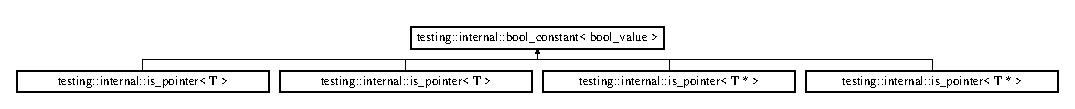
\includegraphics[height=1.021898cm]{structtesting_1_1internal_1_1bool__constant}
\end{center}
\end{figure}
\subsection*{Public Types}
\begin{DoxyCompactItemize}
\item 
\hypertarget{structtesting_1_1internal_1_1bool__constant_aba6d09ecf7eecea6c93480f0d627a167}{}typedef \hyperlink{structtesting_1_1internal_1_1bool__constant}{bool\+\_\+constant}$<$ bool\+\_\+value $>$ {\bfseries type}\label{structtesting_1_1internal_1_1bool__constant_aba6d09ecf7eecea6c93480f0d627a167}

\item 
\hypertarget{structtesting_1_1internal_1_1bool__constant_aba6d09ecf7eecea6c93480f0d627a167}{}typedef \hyperlink{structtesting_1_1internal_1_1bool__constant}{bool\+\_\+constant}$<$ bool\+\_\+value $>$ {\bfseries type}\label{structtesting_1_1internal_1_1bool__constant_aba6d09ecf7eecea6c93480f0d627a167}

\end{DoxyCompactItemize}
\subsection*{Static Public Attributes}
\begin{DoxyCompactItemize}
\item 
\hypertarget{structtesting_1_1internal_1_1bool__constant_a499fba6576296b04d99690a486424b32}{}static const bool {\bfseries value} = bool\+\_\+value\label{structtesting_1_1internal_1_1bool__constant_a499fba6576296b04d99690a486424b32}

\end{DoxyCompactItemize}


The documentation for this struct was generated from the following file\+:\begin{DoxyCompactItemize}
\item 
deps/win32/debug/include/gtest/internal/gtest-\/port.\+h\end{DoxyCompactItemize}

\hypertarget{structstd_1_1tr1_1_1gtest__internal_1_1_by_ref}{}\section{std\+:\+:tr1\+:\+:gtest\+\_\+internal\+:\+:By\+Ref$<$ T $>$ Struct Template Reference}
\label{structstd_1_1tr1_1_1gtest__internal_1_1_by_ref}\index{std\+::tr1\+::gtest\+\_\+internal\+::\+By\+Ref$<$ T $>$@{std\+::tr1\+::gtest\+\_\+internal\+::\+By\+Ref$<$ T $>$}}
\subsection*{Public Types}
\begin{DoxyCompactItemize}
\item 
\hypertarget{structstd_1_1tr1_1_1gtest__internal_1_1_by_ref_ac42ad942ee1cfa86b2abcce9b88ac10e}{}typedef const T \& {\bfseries type}\label{structstd_1_1tr1_1_1gtest__internal_1_1_by_ref_ac42ad942ee1cfa86b2abcce9b88ac10e}

\item 
\hypertarget{structstd_1_1tr1_1_1gtest__internal_1_1_by_ref_ac42ad942ee1cfa86b2abcce9b88ac10e}{}typedef const T \& {\bfseries type}\label{structstd_1_1tr1_1_1gtest__internal_1_1_by_ref_ac42ad942ee1cfa86b2abcce9b88ac10e}

\end{DoxyCompactItemize}


The documentation for this struct was generated from the following file\+:\begin{DoxyCompactItemize}
\item 
deps/win32/debug/include/gtest/internal/gtest-\/tuple.\+h\end{DoxyCompactItemize}

\hypertarget{structstd_1_1tr1_1_1gtest__internal_1_1_by_ref_3_01_t_01_6_01_4}{}\section{std\+:\+:tr1\+:\+:gtest\+\_\+internal\+:\+:By\+Ref$<$ T \& $>$ Struct Template Reference}
\label{structstd_1_1tr1_1_1gtest__internal_1_1_by_ref_3_01_t_01_6_01_4}\index{std\+::tr1\+::gtest\+\_\+internal\+::\+By\+Ref$<$ T \& $>$@{std\+::tr1\+::gtest\+\_\+internal\+::\+By\+Ref$<$ T \& $>$}}
\subsection*{Public Types}
\begin{DoxyCompactItemize}
\item 
\hypertarget{structstd_1_1tr1_1_1gtest__internal_1_1_by_ref_3_01_t_01_6_01_4_a512382574dbdd736320d68e313801122}{}typedef T \& {\bfseries type}\label{structstd_1_1tr1_1_1gtest__internal_1_1_by_ref_3_01_t_01_6_01_4_a512382574dbdd736320d68e313801122}

\item 
\hypertarget{structstd_1_1tr1_1_1gtest__internal_1_1_by_ref_3_01_t_01_6_01_4_a512382574dbdd736320d68e313801122}{}typedef T \& {\bfseries type}\label{structstd_1_1tr1_1_1gtest__internal_1_1_by_ref_3_01_t_01_6_01_4_a512382574dbdd736320d68e313801122}

\end{DoxyCompactItemize}


The documentation for this struct was generated from the following file\+:\begin{DoxyCompactItemize}
\item 
deps/win32/debug/include/gtest/internal/gtest-\/tuple.\+h\end{DoxyCompactItemize}

\hypertarget{structtesting_1_1internal_1_1_compile_assert}{}\section{testing\+:\+:internal\+:\+:Compile\+Assert$<$ bool $>$ Struct Template Reference}
\label{structtesting_1_1internal_1_1_compile_assert}\index{testing\+::internal\+::\+Compile\+Assert$<$ bool $>$@{testing\+::internal\+::\+Compile\+Assert$<$ bool $>$}}


The documentation for this struct was generated from the following file\+:\begin{DoxyCompactItemize}
\item 
deps/win32/debug/include/gtest/internal/gtest-\/port.\+h\end{DoxyCompactItemize}

\hypertarget{structtesting_1_1internal_1_1_compile_assert_types_equal}{}\section{testing\+:\+:internal\+:\+:Compile\+Assert\+Types\+Equal$<$ T1, T2 $>$ Struct Template Reference}
\label{structtesting_1_1internal_1_1_compile_assert_types_equal}\index{testing\+::internal\+::\+Compile\+Assert\+Types\+Equal$<$ T1, T2 $>$@{testing\+::internal\+::\+Compile\+Assert\+Types\+Equal$<$ T1, T2 $>$}}


The documentation for this struct was generated from the following file\+:\begin{DoxyCompactItemize}
\item 
deps/win32/debug/include/gtest/internal/gtest-\/internal.\+h\end{DoxyCompactItemize}

\hypertarget{structtesting_1_1internal_1_1_compile_assert_types_equal_3_01_t_00_01_t_01_4}{}\section{testing\+:\+:internal\+:\+:Compile\+Assert\+Types\+Equal$<$ T, T $>$ Struct Template Reference}
\label{structtesting_1_1internal_1_1_compile_assert_types_equal_3_01_t_00_01_t_01_4}\index{testing\+::internal\+::\+Compile\+Assert\+Types\+Equal$<$ T, T $>$@{testing\+::internal\+::\+Compile\+Assert\+Types\+Equal$<$ T, T $>$}}


The documentation for this struct was generated from the following file\+:\begin{DoxyCompactItemize}
\item 
deps/win32/debug/include/gtest/internal/gtest-\/internal.\+h\end{DoxyCompactItemize}

\hypertarget{structtesting_1_1internal_1_1_const_char_ptr}{}\section{testing\+:\+:internal\+:\+:Const\+Char\+Ptr Struct Reference}
\label{structtesting_1_1internal_1_1_const_char_ptr}\index{testing\+::internal\+::\+Const\+Char\+Ptr@{testing\+::internal\+::\+Const\+Char\+Ptr}}
\subsection*{Public Member Functions}
\begin{DoxyCompactItemize}
\item 
\hypertarget{structtesting_1_1internal_1_1_const_char_ptr_ae94f6453fa679d815994eccc63062907}{}{\bfseries Const\+Char\+Ptr} (const char $\ast$str)\label{structtesting_1_1internal_1_1_const_char_ptr_ae94f6453fa679d815994eccc63062907}

\item 
\hypertarget{structtesting_1_1internal_1_1_const_char_ptr_a891bc286350b81d1a147101c0bae5b1d}{}{\bfseries operator bool} () const \label{structtesting_1_1internal_1_1_const_char_ptr_a891bc286350b81d1a147101c0bae5b1d}

\item 
\hypertarget{structtesting_1_1internal_1_1_const_char_ptr_ae94f6453fa679d815994eccc63062907}{}{\bfseries Const\+Char\+Ptr} (const char $\ast$str)\label{structtesting_1_1internal_1_1_const_char_ptr_ae94f6453fa679d815994eccc63062907}

\item 
\hypertarget{structtesting_1_1internal_1_1_const_char_ptr_a891bc286350b81d1a147101c0bae5b1d}{}{\bfseries operator bool} () const \label{structtesting_1_1internal_1_1_const_char_ptr_a891bc286350b81d1a147101c0bae5b1d}

\end{DoxyCompactItemize}
\subsection*{Public Attributes}
\begin{DoxyCompactItemize}
\item 
\hypertarget{structtesting_1_1internal_1_1_const_char_ptr_a39e195c4214c28f7b1a7dd711742c56e}{}const char $\ast$ {\bfseries value}\label{structtesting_1_1internal_1_1_const_char_ptr_a39e195c4214c28f7b1a7dd711742c56e}

\end{DoxyCompactItemize}


The documentation for this struct was generated from the following file\+:\begin{DoxyCompactItemize}
\item 
deps/win32/debug/include/gtest/internal/gtest-\/internal.\+h\end{DoxyCompactItemize}

\hypertarget{classtesting_1_1_empty_test_event_listener}{}\section{testing\+:\+:Empty\+Test\+Event\+Listener Class Reference}
\label{classtesting_1_1_empty_test_event_listener}\index{testing\+::\+Empty\+Test\+Event\+Listener@{testing\+::\+Empty\+Test\+Event\+Listener}}
Inheritance diagram for testing\+:\+:Empty\+Test\+Event\+Listener\+:\begin{figure}[H]
\begin{center}
\leavevmode
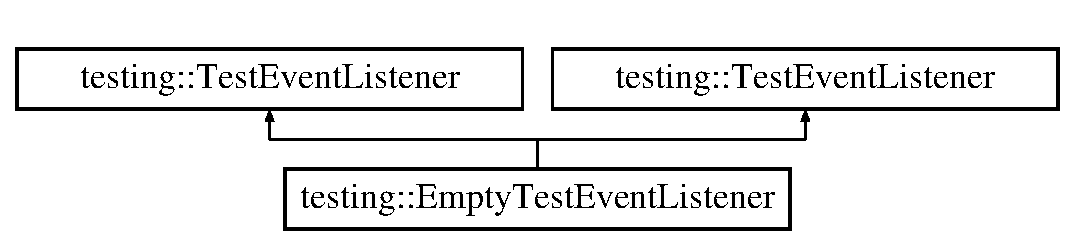
\includegraphics[height=2.000000cm]{classtesting_1_1_empty_test_event_listener}
\end{center}
\end{figure}
\subsection*{Public Member Functions}
\begin{DoxyCompactItemize}
\item 
\hypertarget{classtesting_1_1_empty_test_event_listener_aa3847c8a3c22d8d69a6006dfdd6589fc}{}virtual void {\bfseries On\+Test\+Program\+Start} (const \hyperlink{classtesting_1_1_unit_test}{Unit\+Test} \&)\label{classtesting_1_1_empty_test_event_listener_aa3847c8a3c22d8d69a6006dfdd6589fc}

\item 
\hypertarget{classtesting_1_1_empty_test_event_listener_a836f05829855dc60d13ba99ad712c0dd}{}virtual void {\bfseries On\+Test\+Iteration\+Start} (const \hyperlink{classtesting_1_1_unit_test}{Unit\+Test} \&, int)\label{classtesting_1_1_empty_test_event_listener_a836f05829855dc60d13ba99ad712c0dd}

\item 
\hypertarget{classtesting_1_1_empty_test_event_listener_a156d1965248fbdced6aabacadfa2d63f}{}virtual void {\bfseries On\+Environments\+Set\+Up\+Start} (const \hyperlink{classtesting_1_1_unit_test}{Unit\+Test} \&)\label{classtesting_1_1_empty_test_event_listener_a156d1965248fbdced6aabacadfa2d63f}

\item 
\hypertarget{classtesting_1_1_empty_test_event_listener_abc481c6648d15d4242245195a06f5aa0}{}virtual void {\bfseries On\+Environments\+Set\+Up\+End} (const \hyperlink{classtesting_1_1_unit_test}{Unit\+Test} \&)\label{classtesting_1_1_empty_test_event_listener_abc481c6648d15d4242245195a06f5aa0}

\item 
\hypertarget{classtesting_1_1_empty_test_event_listener_ae4707ed9cc7ace5241bc8ccc4051209b}{}virtual void {\bfseries On\+Test\+Case\+Start} (const \hyperlink{classtesting_1_1_test_case}{Test\+Case} \&)\label{classtesting_1_1_empty_test_event_listener_ae4707ed9cc7ace5241bc8ccc4051209b}

\item 
\hypertarget{classtesting_1_1_empty_test_event_listener_a84fa74cc9ba742f9f847ea405ca84e5e}{}virtual void {\bfseries On\+Test\+Start} (const \hyperlink{classtesting_1_1_test_info}{Test\+Info} \&)\label{classtesting_1_1_empty_test_event_listener_a84fa74cc9ba742f9f847ea405ca84e5e}

\item 
\hypertarget{classtesting_1_1_empty_test_event_listener_a59e7f7d9f2e2d089a6e8c1e2577f4718}{}virtual void {\bfseries On\+Test\+Part\+Result} (const \hyperlink{classtesting_1_1_test_part_result}{Test\+Part\+Result} \&)\label{classtesting_1_1_empty_test_event_listener_a59e7f7d9f2e2d089a6e8c1e2577f4718}

\item 
\hypertarget{classtesting_1_1_empty_test_event_listener_afd58d21005f0d0d0399fb114627545d3}{}virtual void {\bfseries On\+Test\+End} (const \hyperlink{classtesting_1_1_test_info}{Test\+Info} \&)\label{classtesting_1_1_empty_test_event_listener_afd58d21005f0d0d0399fb114627545d3}

\item 
\hypertarget{classtesting_1_1_empty_test_event_listener_a6bec703158283104c4298f7d8a528515}{}virtual void {\bfseries On\+Test\+Case\+End} (const \hyperlink{classtesting_1_1_test_case}{Test\+Case} \&)\label{classtesting_1_1_empty_test_event_listener_a6bec703158283104c4298f7d8a528515}

\item 
\hypertarget{classtesting_1_1_empty_test_event_listener_a00fa1a4ea5831e20746188414268e7c6}{}virtual void {\bfseries On\+Environments\+Tear\+Down\+Start} (const \hyperlink{classtesting_1_1_unit_test}{Unit\+Test} \&)\label{classtesting_1_1_empty_test_event_listener_a00fa1a4ea5831e20746188414268e7c6}

\item 
\hypertarget{classtesting_1_1_empty_test_event_listener_aea64c83c415b33a4c0b0239bafd1438d}{}virtual void {\bfseries On\+Environments\+Tear\+Down\+End} (const \hyperlink{classtesting_1_1_unit_test}{Unit\+Test} \&)\label{classtesting_1_1_empty_test_event_listener_aea64c83c415b33a4c0b0239bafd1438d}

\item 
\hypertarget{classtesting_1_1_empty_test_event_listener_a2253e5a18b3cf7bccd349567a252209d}{}virtual void {\bfseries On\+Test\+Iteration\+End} (const \hyperlink{classtesting_1_1_unit_test}{Unit\+Test} \&, int)\label{classtesting_1_1_empty_test_event_listener_a2253e5a18b3cf7bccd349567a252209d}

\item 
\hypertarget{classtesting_1_1_empty_test_event_listener_a0abcc02bd2331a2e29ad6f4d9daf2a32}{}virtual void {\bfseries On\+Test\+Program\+End} (const \hyperlink{classtesting_1_1_unit_test}{Unit\+Test} \&)\label{classtesting_1_1_empty_test_event_listener_a0abcc02bd2331a2e29ad6f4d9daf2a32}

\item 
\hypertarget{classtesting_1_1_empty_test_event_listener_aa3847c8a3c22d8d69a6006dfdd6589fc}{}virtual void {\bfseries On\+Test\+Program\+Start} (const \hyperlink{classtesting_1_1_unit_test}{Unit\+Test} \&)\label{classtesting_1_1_empty_test_event_listener_aa3847c8a3c22d8d69a6006dfdd6589fc}

\item 
\hypertarget{classtesting_1_1_empty_test_event_listener_a836f05829855dc60d13ba99ad712c0dd}{}virtual void {\bfseries On\+Test\+Iteration\+Start} (const \hyperlink{classtesting_1_1_unit_test}{Unit\+Test} \&, int)\label{classtesting_1_1_empty_test_event_listener_a836f05829855dc60d13ba99ad712c0dd}

\item 
\hypertarget{classtesting_1_1_empty_test_event_listener_a156d1965248fbdced6aabacadfa2d63f}{}virtual void {\bfseries On\+Environments\+Set\+Up\+Start} (const \hyperlink{classtesting_1_1_unit_test}{Unit\+Test} \&)\label{classtesting_1_1_empty_test_event_listener_a156d1965248fbdced6aabacadfa2d63f}

\item 
\hypertarget{classtesting_1_1_empty_test_event_listener_abc481c6648d15d4242245195a06f5aa0}{}virtual void {\bfseries On\+Environments\+Set\+Up\+End} (const \hyperlink{classtesting_1_1_unit_test}{Unit\+Test} \&)\label{classtesting_1_1_empty_test_event_listener_abc481c6648d15d4242245195a06f5aa0}

\item 
\hypertarget{classtesting_1_1_empty_test_event_listener_ae4707ed9cc7ace5241bc8ccc4051209b}{}virtual void {\bfseries On\+Test\+Case\+Start} (const \hyperlink{classtesting_1_1_test_case}{Test\+Case} \&)\label{classtesting_1_1_empty_test_event_listener_ae4707ed9cc7ace5241bc8ccc4051209b}

\item 
\hypertarget{classtesting_1_1_empty_test_event_listener_a84fa74cc9ba742f9f847ea405ca84e5e}{}virtual void {\bfseries On\+Test\+Start} (const \hyperlink{classtesting_1_1_test_info}{Test\+Info} \&)\label{classtesting_1_1_empty_test_event_listener_a84fa74cc9ba742f9f847ea405ca84e5e}

\item 
\hypertarget{classtesting_1_1_empty_test_event_listener_a59e7f7d9f2e2d089a6e8c1e2577f4718}{}virtual void {\bfseries On\+Test\+Part\+Result} (const \hyperlink{classtesting_1_1_test_part_result}{Test\+Part\+Result} \&)\label{classtesting_1_1_empty_test_event_listener_a59e7f7d9f2e2d089a6e8c1e2577f4718}

\item 
\hypertarget{classtesting_1_1_empty_test_event_listener_afd58d21005f0d0d0399fb114627545d3}{}virtual void {\bfseries On\+Test\+End} (const \hyperlink{classtesting_1_1_test_info}{Test\+Info} \&)\label{classtesting_1_1_empty_test_event_listener_afd58d21005f0d0d0399fb114627545d3}

\item 
\hypertarget{classtesting_1_1_empty_test_event_listener_a6bec703158283104c4298f7d8a528515}{}virtual void {\bfseries On\+Test\+Case\+End} (const \hyperlink{classtesting_1_1_test_case}{Test\+Case} \&)\label{classtesting_1_1_empty_test_event_listener_a6bec703158283104c4298f7d8a528515}

\item 
\hypertarget{classtesting_1_1_empty_test_event_listener_a00fa1a4ea5831e20746188414268e7c6}{}virtual void {\bfseries On\+Environments\+Tear\+Down\+Start} (const \hyperlink{classtesting_1_1_unit_test}{Unit\+Test} \&)\label{classtesting_1_1_empty_test_event_listener_a00fa1a4ea5831e20746188414268e7c6}

\item 
\hypertarget{classtesting_1_1_empty_test_event_listener_aea64c83c415b33a4c0b0239bafd1438d}{}virtual void {\bfseries On\+Environments\+Tear\+Down\+End} (const \hyperlink{classtesting_1_1_unit_test}{Unit\+Test} \&)\label{classtesting_1_1_empty_test_event_listener_aea64c83c415b33a4c0b0239bafd1438d}

\item 
\hypertarget{classtesting_1_1_empty_test_event_listener_a2253e5a18b3cf7bccd349567a252209d}{}virtual void {\bfseries On\+Test\+Iteration\+End} (const \hyperlink{classtesting_1_1_unit_test}{Unit\+Test} \&, int)\label{classtesting_1_1_empty_test_event_listener_a2253e5a18b3cf7bccd349567a252209d}

\item 
\hypertarget{classtesting_1_1_empty_test_event_listener_a0abcc02bd2331a2e29ad6f4d9daf2a32}{}virtual void {\bfseries On\+Test\+Program\+End} (const \hyperlink{classtesting_1_1_unit_test}{Unit\+Test} \&)\label{classtesting_1_1_empty_test_event_listener_a0abcc02bd2331a2e29ad6f4d9daf2a32}

\end{DoxyCompactItemize}


The documentation for this class was generated from the following file\+:\begin{DoxyCompactItemize}
\item 
deps/win32/debug/include/gtest/gtest.\+h\end{DoxyCompactItemize}

\hypertarget{structtesting_1_1internal_1_1_enable_if}{}\section{testing\+:\+:internal\+:\+:Enable\+If$<$ bool $>$ Struct Template Reference}
\label{structtesting_1_1internal_1_1_enable_if}\index{testing\+::internal\+::\+Enable\+If$<$ bool $>$@{testing\+::internal\+::\+Enable\+If$<$ bool $>$}}


The documentation for this struct was generated from the following file\+:\begin{DoxyCompactItemize}
\item 
deps/win32/debug/include/gtest/internal/gtest-\/internal.\+h\end{DoxyCompactItemize}

\hypertarget{structtesting_1_1internal_1_1_enable_if_3_01true_01_4}{}\section{testing\+:\+:internal\+:\+:Enable\+If$<$ true $>$ Struct Template Reference}
\label{structtesting_1_1internal_1_1_enable_if_3_01true_01_4}\index{testing\+::internal\+::\+Enable\+If$<$ true $>$@{testing\+::internal\+::\+Enable\+If$<$ true $>$}}
\subsection*{Public Types}
\begin{DoxyCompactItemize}
\item 
\hypertarget{structtesting_1_1internal_1_1_enable_if_3_01true_01_4_a9398d803f1fdd99ff41823746f6299ff}{}typedef void {\bfseries type}\label{structtesting_1_1internal_1_1_enable_if_3_01true_01_4_a9398d803f1fdd99ff41823746f6299ff}

\item 
\hypertarget{structtesting_1_1internal_1_1_enable_if_3_01true_01_4_a9398d803f1fdd99ff41823746f6299ff}{}typedef void {\bfseries type}\label{structtesting_1_1internal_1_1_enable_if_3_01true_01_4_a9398d803f1fdd99ff41823746f6299ff}

\end{DoxyCompactItemize}


The documentation for this struct was generated from the following file\+:\begin{DoxyCompactItemize}
\item 
deps/win32/debug/include/gtest/internal/gtest-\/internal.\+h\end{DoxyCompactItemize}

\hypertarget{classtesting_1_1_environment}{}\section{testing\+:\+:Environment Class Reference}
\label{classtesting_1_1_environment}\index{testing\+::\+Environment@{testing\+::\+Environment}}
\subsection*{Public Member Functions}
\begin{DoxyCompactItemize}
\item 
\hypertarget{classtesting_1_1_environment_a1bf8cafaa9d4eba9feb98655ee434eb3}{}virtual void {\bfseries Set\+Up} ()\label{classtesting_1_1_environment_a1bf8cafaa9d4eba9feb98655ee434eb3}

\item 
\hypertarget{classtesting_1_1_environment_a039bdaa705c46b9b88234cf4d3bb6254}{}virtual void {\bfseries Tear\+Down} ()\label{classtesting_1_1_environment_a039bdaa705c46b9b88234cf4d3bb6254}

\item 
\hypertarget{classtesting_1_1_environment_a1bf8cafaa9d4eba9feb98655ee434eb3}{}virtual void {\bfseries Set\+Up} ()\label{classtesting_1_1_environment_a1bf8cafaa9d4eba9feb98655ee434eb3}

\item 
\hypertarget{classtesting_1_1_environment_a039bdaa705c46b9b88234cf4d3bb6254}{}virtual void {\bfseries Tear\+Down} ()\label{classtesting_1_1_environment_a039bdaa705c46b9b88234cf4d3bb6254}

\end{DoxyCompactItemize}


The documentation for this class was generated from the following file\+:\begin{DoxyCompactItemize}
\item 
deps/win32/debug/include/gtest/gtest.\+h\end{DoxyCompactItemize}

\hypertarget{classtesting_1_1internal_1_1_eq_helper}{}\section{testing\+:\+:internal\+:\+:Eq\+Helper$<$ lhs\+\_\+is\+\_\+null\+\_\+literal $>$ Class Template Reference}
\label{classtesting_1_1internal_1_1_eq_helper}\index{testing\+::internal\+::\+Eq\+Helper$<$ lhs\+\_\+is\+\_\+null\+\_\+literal $>$@{testing\+::internal\+::\+Eq\+Helper$<$ lhs\+\_\+is\+\_\+null\+\_\+literal $>$}}
\subsection*{Static Public Member Functions}
\begin{DoxyCompactItemize}
\item 
\hypertarget{classtesting_1_1internal_1_1_eq_helper_ac2977ed90cd3c88607f804e43b86b92c}{}{\footnotesize template$<$typename T1 , typename T2 $>$ }\\static \hyperlink{classtesting_1_1_assertion_result}{Assertion\+Result} {\bfseries Compare} (const char $\ast$expected\+\_\+expression, const char $\ast$actual\+\_\+expression, const T1 \&expected, const T2 \&actual)\label{classtesting_1_1internal_1_1_eq_helper_ac2977ed90cd3c88607f804e43b86b92c}

\item 
\hypertarget{classtesting_1_1internal_1_1_eq_helper_a3de996954b41d484c065ed824fe7eac9}{}static \hyperlink{classtesting_1_1_assertion_result}{Assertion\+Result} {\bfseries Compare} (const char $\ast$expected\+\_\+expression, const char $\ast$actual\+\_\+expression, Biggest\+Int expected, Biggest\+Int actual)\label{classtesting_1_1internal_1_1_eq_helper_a3de996954b41d484c065ed824fe7eac9}

\item 
\hypertarget{classtesting_1_1internal_1_1_eq_helper_ac2977ed90cd3c88607f804e43b86b92c}{}{\footnotesize template$<$typename T1 , typename T2 $>$ }\\static \hyperlink{classtesting_1_1_assertion_result}{Assertion\+Result} {\bfseries Compare} (const char $\ast$expected\+\_\+expression, const char $\ast$actual\+\_\+expression, const T1 \&expected, const T2 \&actual)\label{classtesting_1_1internal_1_1_eq_helper_ac2977ed90cd3c88607f804e43b86b92c}

\item 
\hypertarget{classtesting_1_1internal_1_1_eq_helper_a3de996954b41d484c065ed824fe7eac9}{}static \hyperlink{classtesting_1_1_assertion_result}{Assertion\+Result} {\bfseries Compare} (const char $\ast$expected\+\_\+expression, const char $\ast$actual\+\_\+expression, Biggest\+Int expected, Biggest\+Int actual)\label{classtesting_1_1internal_1_1_eq_helper_a3de996954b41d484c065ed824fe7eac9}

\end{DoxyCompactItemize}


The documentation for this class was generated from the following file\+:\begin{DoxyCompactItemize}
\item 
deps/win32/debug/include/gtest/gtest.\+h\end{DoxyCompactItemize}

\hypertarget{classtesting_1_1internal_1_1_eq_helper_3_01true_01_4}{}\section{testing\+:\+:internal\+:\+:Eq\+Helper$<$ true $>$ Class Template Reference}
\label{classtesting_1_1internal_1_1_eq_helper_3_01true_01_4}\index{testing\+::internal\+::\+Eq\+Helper$<$ true $>$@{testing\+::internal\+::\+Eq\+Helper$<$ true $>$}}
\subsection*{Static Public Member Functions}
\begin{DoxyCompactItemize}
\item 
\hypertarget{classtesting_1_1internal_1_1_eq_helper_3_01true_01_4_a70d6d7e3cb1df06ad6114f25e843fd6d}{}{\footnotesize template$<$typename T1 , typename T2 $>$ }\\static \hyperlink{classtesting_1_1_assertion_result}{Assertion\+Result} {\bfseries Compare} (const char $\ast$expected\+\_\+expression, const char $\ast$actual\+\_\+expression, const T1 \&expected, const T2 \&actual, typename \hyperlink{structtesting_1_1internal_1_1_enable_if}{Enable\+If}$<$!\hyperlink{structtesting_1_1internal_1_1is__pointer}{is\+\_\+pointer}$<$ T2 $>$\+::value $>$\+::type $\ast$=0)\label{classtesting_1_1internal_1_1_eq_helper_3_01true_01_4_a70d6d7e3cb1df06ad6114f25e843fd6d}

\item 
\hypertarget{classtesting_1_1internal_1_1_eq_helper_3_01true_01_4_ab38e840297adb48f18767a1a99187fb3}{}{\footnotesize template$<$typename T $>$ }\\static \hyperlink{classtesting_1_1_assertion_result}{Assertion\+Result} {\bfseries Compare} (const char $\ast$expected\+\_\+expression, const char $\ast$actual\+\_\+expression, Secret $\ast$, T $\ast$actual)\label{classtesting_1_1internal_1_1_eq_helper_3_01true_01_4_ab38e840297adb48f18767a1a99187fb3}

\item 
\hypertarget{classtesting_1_1internal_1_1_eq_helper_3_01true_01_4_a70d6d7e3cb1df06ad6114f25e843fd6d}{}{\footnotesize template$<$typename T1 , typename T2 $>$ }\\static \hyperlink{classtesting_1_1_assertion_result}{Assertion\+Result} {\bfseries Compare} (const char $\ast$expected\+\_\+expression, const char $\ast$actual\+\_\+expression, const T1 \&expected, const T2 \&actual, typename \hyperlink{structtesting_1_1internal_1_1_enable_if}{Enable\+If}$<$!\hyperlink{structtesting_1_1internal_1_1is__pointer}{is\+\_\+pointer}$<$ T2 $>$\+::value $>$\+::type $\ast$=0)\label{classtesting_1_1internal_1_1_eq_helper_3_01true_01_4_a70d6d7e3cb1df06ad6114f25e843fd6d}

\item 
\hypertarget{classtesting_1_1internal_1_1_eq_helper_3_01true_01_4_ab38e840297adb48f18767a1a99187fb3}{}{\footnotesize template$<$typename T $>$ }\\static \hyperlink{classtesting_1_1_assertion_result}{Assertion\+Result} {\bfseries Compare} (const char $\ast$expected\+\_\+expression, const char $\ast$actual\+\_\+expression, Secret $\ast$, T $\ast$actual)\label{classtesting_1_1internal_1_1_eq_helper_3_01true_01_4_ab38e840297adb48f18767a1a99187fb3}

\end{DoxyCompactItemize}


The documentation for this class was generated from the following file\+:\begin{DoxyCompactItemize}
\item 
deps/win32/debug/include/gtest/gtest.\+h\end{DoxyCompactItemize}

\hypertarget{classtesting_1_1internal_1_1_file_path}{}\section{testing\+:\+:internal\+:\+:File\+Path Class Reference}
\label{classtesting_1_1internal_1_1_file_path}\index{testing\+::internal\+::\+File\+Path@{testing\+::internal\+::\+File\+Path}}
\subsection*{Public Member Functions}
\begin{DoxyCompactItemize}
\item 
\hypertarget{classtesting_1_1internal_1_1_file_path_ae9efd0fee56c6e3e2d659b464250b112}{}{\bfseries File\+Path} (const \hyperlink{classtesting_1_1internal_1_1_file_path}{File\+Path} \&rhs)\label{classtesting_1_1internal_1_1_file_path_ae9efd0fee56c6e3e2d659b464250b112}

\item 
\hypertarget{classtesting_1_1internal_1_1_file_path_a9fc072b140aa0652a7022fb809fe3abe}{}{\bfseries File\+Path} (const std\+::string \&pathname)\label{classtesting_1_1internal_1_1_file_path_a9fc072b140aa0652a7022fb809fe3abe}

\item 
\hypertarget{classtesting_1_1internal_1_1_file_path_a8d9c1bafb90f10bcd5611a54d8f326ef}{}\hyperlink{classtesting_1_1internal_1_1_file_path}{File\+Path} \& {\bfseries operator=} (const \hyperlink{classtesting_1_1internal_1_1_file_path}{File\+Path} \&rhs)\label{classtesting_1_1internal_1_1_file_path_a8d9c1bafb90f10bcd5611a54d8f326ef}

\item 
\hypertarget{classtesting_1_1internal_1_1_file_path_a15a42de7518e89254e0640dd9317d5f7}{}void {\bfseries Set} (const \hyperlink{classtesting_1_1internal_1_1_file_path}{File\+Path} \&rhs)\label{classtesting_1_1internal_1_1_file_path_a15a42de7518e89254e0640dd9317d5f7}

\item 
\hypertarget{classtesting_1_1internal_1_1_file_path_a7c544a30af67e2da5ce7e625f8402818}{}const std\+::string \& {\bfseries string} () const \label{classtesting_1_1internal_1_1_file_path_a7c544a30af67e2da5ce7e625f8402818}

\item 
\hypertarget{classtesting_1_1internal_1_1_file_path_a85297234dac0acd936632dff8634c2b9}{}const char $\ast$ {\bfseries c\+\_\+str} () const \label{classtesting_1_1internal_1_1_file_path_a85297234dac0acd936632dff8634c2b9}

\item 
\hypertarget{classtesting_1_1internal_1_1_file_path_a44543ff34ae757038ab20925659b447a}{}bool {\bfseries Is\+Empty} () const \label{classtesting_1_1internal_1_1_file_path_a44543ff34ae757038ab20925659b447a}

\item 
\hypertarget{classtesting_1_1internal_1_1_file_path_a952e1b2a9909cdeaf25de5fcdf069b3a}{}\hyperlink{classtesting_1_1internal_1_1_file_path}{File\+Path} {\bfseries Remove\+Trailing\+Path\+Separator} () const \label{classtesting_1_1internal_1_1_file_path_a952e1b2a9909cdeaf25de5fcdf069b3a}

\item 
\hypertarget{classtesting_1_1internal_1_1_file_path_a2852e5a759ff2e2620c7317b8121d757}{}\hyperlink{classtesting_1_1internal_1_1_file_path}{File\+Path} {\bfseries Remove\+Directory\+Name} () const \label{classtesting_1_1internal_1_1_file_path_a2852e5a759ff2e2620c7317b8121d757}

\item 
\hypertarget{classtesting_1_1internal_1_1_file_path_aed3abcd0b8a7f6ed1ff0e7743ef8bf1e}{}\hyperlink{classtesting_1_1internal_1_1_file_path}{File\+Path} {\bfseries Remove\+File\+Name} () const \label{classtesting_1_1internal_1_1_file_path_aed3abcd0b8a7f6ed1ff0e7743ef8bf1e}

\item 
\hypertarget{classtesting_1_1internal_1_1_file_path_ab2a25cc916c111597b94d006aa973c3d}{}\hyperlink{classtesting_1_1internal_1_1_file_path}{File\+Path} {\bfseries Remove\+Extension} (const char $\ast$extension) const \label{classtesting_1_1internal_1_1_file_path_ab2a25cc916c111597b94d006aa973c3d}

\item 
\hypertarget{classtesting_1_1internal_1_1_file_path_afccf35a45e209c22e68c6f8e86036c12}{}bool {\bfseries Create\+Directories\+Recursively} () const \label{classtesting_1_1internal_1_1_file_path_afccf35a45e209c22e68c6f8e86036c12}

\item 
\hypertarget{classtesting_1_1internal_1_1_file_path_a303cdda61bee6e8a0b0303e8fc857e36}{}bool {\bfseries Create\+Folder} () const \label{classtesting_1_1internal_1_1_file_path_a303cdda61bee6e8a0b0303e8fc857e36}

\item 
\hypertarget{classtesting_1_1internal_1_1_file_path_a3548d3ead0e94701669afc64d765ece7}{}bool {\bfseries File\+Or\+Directory\+Exists} () const \label{classtesting_1_1internal_1_1_file_path_a3548d3ead0e94701669afc64d765ece7}

\item 
\hypertarget{classtesting_1_1internal_1_1_file_path_a3546b3f926935fefddb9a808e7e2be47}{}bool {\bfseries Directory\+Exists} () const \label{classtesting_1_1internal_1_1_file_path_a3546b3f926935fefddb9a808e7e2be47}

\item 
\hypertarget{classtesting_1_1internal_1_1_file_path_a918336f16efa8e07d4b94192d6a89f44}{}bool {\bfseries Is\+Directory} () const \label{classtesting_1_1internal_1_1_file_path_a918336f16efa8e07d4b94192d6a89f44}

\item 
\hypertarget{classtesting_1_1internal_1_1_file_path_a7d31c82f3f979c54e5a985382b52feb1}{}bool {\bfseries Is\+Root\+Directory} () const \label{classtesting_1_1internal_1_1_file_path_a7d31c82f3f979c54e5a985382b52feb1}

\item 
\hypertarget{classtesting_1_1internal_1_1_file_path_a720a5f0fd00f3e98d6f3518f4dadfff5}{}bool {\bfseries Is\+Absolute\+Path} () const \label{classtesting_1_1internal_1_1_file_path_a720a5f0fd00f3e98d6f3518f4dadfff5}

\item 
\hypertarget{classtesting_1_1internal_1_1_file_path_ae9efd0fee56c6e3e2d659b464250b112}{}{\bfseries File\+Path} (const \hyperlink{classtesting_1_1internal_1_1_file_path}{File\+Path} \&rhs)\label{classtesting_1_1internal_1_1_file_path_ae9efd0fee56c6e3e2d659b464250b112}

\item 
\hypertarget{classtesting_1_1internal_1_1_file_path_a9fc072b140aa0652a7022fb809fe3abe}{}{\bfseries File\+Path} (const std\+::string \&pathname)\label{classtesting_1_1internal_1_1_file_path_a9fc072b140aa0652a7022fb809fe3abe}

\item 
\hypertarget{classtesting_1_1internal_1_1_file_path_a8d9c1bafb90f10bcd5611a54d8f326ef}{}\hyperlink{classtesting_1_1internal_1_1_file_path}{File\+Path} \& {\bfseries operator=} (const \hyperlink{classtesting_1_1internal_1_1_file_path}{File\+Path} \&rhs)\label{classtesting_1_1internal_1_1_file_path_a8d9c1bafb90f10bcd5611a54d8f326ef}

\item 
\hypertarget{classtesting_1_1internal_1_1_file_path_a15a42de7518e89254e0640dd9317d5f7}{}void {\bfseries Set} (const \hyperlink{classtesting_1_1internal_1_1_file_path}{File\+Path} \&rhs)\label{classtesting_1_1internal_1_1_file_path_a15a42de7518e89254e0640dd9317d5f7}

\item 
\hypertarget{classtesting_1_1internal_1_1_file_path_a7c544a30af67e2da5ce7e625f8402818}{}const std\+::string \& {\bfseries string} () const \label{classtesting_1_1internal_1_1_file_path_a7c544a30af67e2da5ce7e625f8402818}

\item 
\hypertarget{classtesting_1_1internal_1_1_file_path_a85297234dac0acd936632dff8634c2b9}{}const char $\ast$ {\bfseries c\+\_\+str} () const \label{classtesting_1_1internal_1_1_file_path_a85297234dac0acd936632dff8634c2b9}

\item 
\hypertarget{classtesting_1_1internal_1_1_file_path_a44543ff34ae757038ab20925659b447a}{}bool {\bfseries Is\+Empty} () const \label{classtesting_1_1internal_1_1_file_path_a44543ff34ae757038ab20925659b447a}

\item 
\hypertarget{classtesting_1_1internal_1_1_file_path_a952e1b2a9909cdeaf25de5fcdf069b3a}{}\hyperlink{classtesting_1_1internal_1_1_file_path}{File\+Path} {\bfseries Remove\+Trailing\+Path\+Separator} () const \label{classtesting_1_1internal_1_1_file_path_a952e1b2a9909cdeaf25de5fcdf069b3a}

\item 
\hypertarget{classtesting_1_1internal_1_1_file_path_a2852e5a759ff2e2620c7317b8121d757}{}\hyperlink{classtesting_1_1internal_1_1_file_path}{File\+Path} {\bfseries Remove\+Directory\+Name} () const \label{classtesting_1_1internal_1_1_file_path_a2852e5a759ff2e2620c7317b8121d757}

\item 
\hypertarget{classtesting_1_1internal_1_1_file_path_aed3abcd0b8a7f6ed1ff0e7743ef8bf1e}{}\hyperlink{classtesting_1_1internal_1_1_file_path}{File\+Path} {\bfseries Remove\+File\+Name} () const \label{classtesting_1_1internal_1_1_file_path_aed3abcd0b8a7f6ed1ff0e7743ef8bf1e}

\item 
\hypertarget{classtesting_1_1internal_1_1_file_path_ab2a25cc916c111597b94d006aa973c3d}{}\hyperlink{classtesting_1_1internal_1_1_file_path}{File\+Path} {\bfseries Remove\+Extension} (const char $\ast$extension) const \label{classtesting_1_1internal_1_1_file_path_ab2a25cc916c111597b94d006aa973c3d}

\item 
\hypertarget{classtesting_1_1internal_1_1_file_path_afccf35a45e209c22e68c6f8e86036c12}{}bool {\bfseries Create\+Directories\+Recursively} () const \label{classtesting_1_1internal_1_1_file_path_afccf35a45e209c22e68c6f8e86036c12}

\item 
\hypertarget{classtesting_1_1internal_1_1_file_path_a303cdda61bee6e8a0b0303e8fc857e36}{}bool {\bfseries Create\+Folder} () const \label{classtesting_1_1internal_1_1_file_path_a303cdda61bee6e8a0b0303e8fc857e36}

\item 
\hypertarget{classtesting_1_1internal_1_1_file_path_a3548d3ead0e94701669afc64d765ece7}{}bool {\bfseries File\+Or\+Directory\+Exists} () const \label{classtesting_1_1internal_1_1_file_path_a3548d3ead0e94701669afc64d765ece7}

\item 
\hypertarget{classtesting_1_1internal_1_1_file_path_a3546b3f926935fefddb9a808e7e2be47}{}bool {\bfseries Directory\+Exists} () const \label{classtesting_1_1internal_1_1_file_path_a3546b3f926935fefddb9a808e7e2be47}

\item 
\hypertarget{classtesting_1_1internal_1_1_file_path_a918336f16efa8e07d4b94192d6a89f44}{}bool {\bfseries Is\+Directory} () const \label{classtesting_1_1internal_1_1_file_path_a918336f16efa8e07d4b94192d6a89f44}

\item 
\hypertarget{classtesting_1_1internal_1_1_file_path_a7d31c82f3f979c54e5a985382b52feb1}{}bool {\bfseries Is\+Root\+Directory} () const \label{classtesting_1_1internal_1_1_file_path_a7d31c82f3f979c54e5a985382b52feb1}

\item 
\hypertarget{classtesting_1_1internal_1_1_file_path_a720a5f0fd00f3e98d6f3518f4dadfff5}{}bool {\bfseries Is\+Absolute\+Path} () const \label{classtesting_1_1internal_1_1_file_path_a720a5f0fd00f3e98d6f3518f4dadfff5}

\end{DoxyCompactItemize}
\subsection*{Static Public Member Functions}
\begin{DoxyCompactItemize}
\item 
\hypertarget{classtesting_1_1internal_1_1_file_path_a0f7b48e493656679cb82a2b679620c4e}{}static \hyperlink{classtesting_1_1internal_1_1_file_path}{File\+Path} {\bfseries Get\+Current\+Dir} ()\label{classtesting_1_1internal_1_1_file_path_a0f7b48e493656679cb82a2b679620c4e}

\item 
\hypertarget{classtesting_1_1internal_1_1_file_path_a1e7793eaae21c6629afe8be11064b111}{}static \hyperlink{classtesting_1_1internal_1_1_file_path}{File\+Path} {\bfseries Make\+File\+Name} (const \hyperlink{classtesting_1_1internal_1_1_file_path}{File\+Path} \&directory, const \hyperlink{classtesting_1_1internal_1_1_file_path}{File\+Path} \&base\+\_\+name, int number, const char $\ast$extension)\label{classtesting_1_1internal_1_1_file_path_a1e7793eaae21c6629afe8be11064b111}

\item 
\hypertarget{classtesting_1_1internal_1_1_file_path_ad58aa6d8b160d0ba0b661f56f0980e26}{}static \hyperlink{classtesting_1_1internal_1_1_file_path}{File\+Path} {\bfseries Concat\+Paths} (const \hyperlink{classtesting_1_1internal_1_1_file_path}{File\+Path} \&directory, const \hyperlink{classtesting_1_1internal_1_1_file_path}{File\+Path} \&relative\+\_\+path)\label{classtesting_1_1internal_1_1_file_path_ad58aa6d8b160d0ba0b661f56f0980e26}

\item 
\hypertarget{classtesting_1_1internal_1_1_file_path_ab22637ea53e3918ec814dc6a5fecd1f9}{}static \hyperlink{classtesting_1_1internal_1_1_file_path}{File\+Path} {\bfseries Generate\+Unique\+File\+Name} (const \hyperlink{classtesting_1_1internal_1_1_file_path}{File\+Path} \&directory, const \hyperlink{classtesting_1_1internal_1_1_file_path}{File\+Path} \&base\+\_\+name, const char $\ast$extension)\label{classtesting_1_1internal_1_1_file_path_ab22637ea53e3918ec814dc6a5fecd1f9}

\item 
\hypertarget{classtesting_1_1internal_1_1_file_path_a0f7b48e493656679cb82a2b679620c4e}{}static \hyperlink{classtesting_1_1internal_1_1_file_path}{File\+Path} {\bfseries Get\+Current\+Dir} ()\label{classtesting_1_1internal_1_1_file_path_a0f7b48e493656679cb82a2b679620c4e}

\item 
\hypertarget{classtesting_1_1internal_1_1_file_path_a1e7793eaae21c6629afe8be11064b111}{}static \hyperlink{classtesting_1_1internal_1_1_file_path}{File\+Path} {\bfseries Make\+File\+Name} (const \hyperlink{classtesting_1_1internal_1_1_file_path}{File\+Path} \&directory, const \hyperlink{classtesting_1_1internal_1_1_file_path}{File\+Path} \&base\+\_\+name, int number, const char $\ast$extension)\label{classtesting_1_1internal_1_1_file_path_a1e7793eaae21c6629afe8be11064b111}

\item 
\hypertarget{classtesting_1_1internal_1_1_file_path_ad58aa6d8b160d0ba0b661f56f0980e26}{}static \hyperlink{classtesting_1_1internal_1_1_file_path}{File\+Path} {\bfseries Concat\+Paths} (const \hyperlink{classtesting_1_1internal_1_1_file_path}{File\+Path} \&directory, const \hyperlink{classtesting_1_1internal_1_1_file_path}{File\+Path} \&relative\+\_\+path)\label{classtesting_1_1internal_1_1_file_path_ad58aa6d8b160d0ba0b661f56f0980e26}

\item 
\hypertarget{classtesting_1_1internal_1_1_file_path_ab22637ea53e3918ec814dc6a5fecd1f9}{}static \hyperlink{classtesting_1_1internal_1_1_file_path}{File\+Path} {\bfseries Generate\+Unique\+File\+Name} (const \hyperlink{classtesting_1_1internal_1_1_file_path}{File\+Path} \&directory, const \hyperlink{classtesting_1_1internal_1_1_file_path}{File\+Path} \&base\+\_\+name, const char $\ast$extension)\label{classtesting_1_1internal_1_1_file_path_ab22637ea53e3918ec814dc6a5fecd1f9}

\end{DoxyCompactItemize}


The documentation for this class was generated from the following file\+:\begin{DoxyCompactItemize}
\item 
deps/win32/debug/include/gtest/internal/gtest-\/filepath.\+h\end{DoxyCompactItemize}

\hypertarget{classmm_1_1_file_utils}{}\section{mm\+:\+:File\+Utils Class Reference}
\label{classmm_1_1_file_utils}\index{mm\+::\+File\+Utils@{mm\+::\+File\+Utils}}
\subsection*{Static Public Member Functions}
\begin{DoxyCompactItemize}
\item 
\hypertarget{classmm_1_1_file_utils_a1dd11f27342fbe994abd8f83762666f5}{}static std\+::string {\bfseries read\+Text\+File} (const std\+::string \&filename)\label{classmm_1_1_file_utils_a1dd11f27342fbe994abd8f83762666f5}

\end{DoxyCompactItemize}


The documentation for this class was generated from the following files\+:\begin{DoxyCompactItemize}
\item 
src/core/mm\+\_\+utils.\+h\item 
src/core/mm\+\_\+utils.\+cc\end{DoxyCompactItemize}

\hypertarget{classtesting_1_1internal_1_1_floating_point}{}\section{testing\+:\+:internal\+:\+:Floating\+Point$<$ Raw\+Type $>$ Class Template Reference}
\label{classtesting_1_1internal_1_1_floating_point}\index{testing\+::internal\+::\+Floating\+Point$<$ Raw\+Type $>$@{testing\+::internal\+::\+Floating\+Point$<$ Raw\+Type $>$}}
\subsection*{Public Types}
\begin{DoxyCompactItemize}
\item 
\hypertarget{classtesting_1_1internal_1_1_floating_point_abf228bf6cd48f12c8b44c85b4971a731}{}typedef \hyperlink{classtesting_1_1internal_1_1_type_with_size}{Type\+With\+Size}$<$ sizeof(Raw\+Type)$>$\+::U\+Int {\bfseries Bits}\label{classtesting_1_1internal_1_1_floating_point_abf228bf6cd48f12c8b44c85b4971a731}

\item 
\hypertarget{classtesting_1_1internal_1_1_floating_point_abf228bf6cd48f12c8b44c85b4971a731}{}typedef \hyperlink{classtesting_1_1internal_1_1_type_with_size}{Type\+With\+Size}$<$ sizeof(Raw\+Type)$>$\+::U\+Int {\bfseries Bits}\label{classtesting_1_1internal_1_1_floating_point_abf228bf6cd48f12c8b44c85b4971a731}

\end{DoxyCompactItemize}
\subsection*{Public Member Functions}
\begin{DoxyCompactItemize}
\item 
\hypertarget{classtesting_1_1internal_1_1_floating_point_a0dabf840863e0df84046f171c891fe71}{}{\bfseries Floating\+Point} (const Raw\+Type \&x)\label{classtesting_1_1internal_1_1_floating_point_a0dabf840863e0df84046f171c891fe71}

\item 
\hypertarget{classtesting_1_1internal_1_1_floating_point_abead51f16ec6ea84360a976da1cd1387}{}const Bits \& {\bfseries bits} () const \label{classtesting_1_1internal_1_1_floating_point_abead51f16ec6ea84360a976da1cd1387}

\item 
\hypertarget{classtesting_1_1internal_1_1_floating_point_af53c50b85408c582540d6244c026ce2b}{}Bits {\bfseries exponent\+\_\+bits} () const \label{classtesting_1_1internal_1_1_floating_point_af53c50b85408c582540d6244c026ce2b}

\item 
\hypertarget{classtesting_1_1internal_1_1_floating_point_aa0167b7b10a934b743ba3c1f47421e63}{}Bits {\bfseries fraction\+\_\+bits} () const \label{classtesting_1_1internal_1_1_floating_point_aa0167b7b10a934b743ba3c1f47421e63}

\item 
\hypertarget{classtesting_1_1internal_1_1_floating_point_a6176cc4d443724477f2799bcbd9f020a}{}Bits {\bfseries sign\+\_\+bit} () const \label{classtesting_1_1internal_1_1_floating_point_a6176cc4d443724477f2799bcbd9f020a}

\item 
\hypertarget{classtesting_1_1internal_1_1_floating_point_aaef2fd2cd8cdf791206a5e9fed8ef90d}{}bool {\bfseries is\+\_\+nan} () const \label{classtesting_1_1internal_1_1_floating_point_aaef2fd2cd8cdf791206a5e9fed8ef90d}

\item 
\hypertarget{classtesting_1_1internal_1_1_floating_point_adb0fe9ab1d9e5288f8e5550234211166}{}bool {\bfseries Almost\+Equals} (const \hyperlink{classtesting_1_1internal_1_1_floating_point}{Floating\+Point} \&rhs) const \label{classtesting_1_1internal_1_1_floating_point_adb0fe9ab1d9e5288f8e5550234211166}

\item 
\hypertarget{classtesting_1_1internal_1_1_floating_point_a0dabf840863e0df84046f171c891fe71}{}{\bfseries Floating\+Point} (const Raw\+Type \&x)\label{classtesting_1_1internal_1_1_floating_point_a0dabf840863e0df84046f171c891fe71}

\item 
\hypertarget{classtesting_1_1internal_1_1_floating_point_abead51f16ec6ea84360a976da1cd1387}{}const Bits \& {\bfseries bits} () const \label{classtesting_1_1internal_1_1_floating_point_abead51f16ec6ea84360a976da1cd1387}

\item 
\hypertarget{classtesting_1_1internal_1_1_floating_point_af53c50b85408c582540d6244c026ce2b}{}Bits {\bfseries exponent\+\_\+bits} () const \label{classtesting_1_1internal_1_1_floating_point_af53c50b85408c582540d6244c026ce2b}

\item 
\hypertarget{classtesting_1_1internal_1_1_floating_point_aa0167b7b10a934b743ba3c1f47421e63}{}Bits {\bfseries fraction\+\_\+bits} () const \label{classtesting_1_1internal_1_1_floating_point_aa0167b7b10a934b743ba3c1f47421e63}

\item 
\hypertarget{classtesting_1_1internal_1_1_floating_point_a6176cc4d443724477f2799bcbd9f020a}{}Bits {\bfseries sign\+\_\+bit} () const \label{classtesting_1_1internal_1_1_floating_point_a6176cc4d443724477f2799bcbd9f020a}

\item 
\hypertarget{classtesting_1_1internal_1_1_floating_point_aaef2fd2cd8cdf791206a5e9fed8ef90d}{}bool {\bfseries is\+\_\+nan} () const \label{classtesting_1_1internal_1_1_floating_point_aaef2fd2cd8cdf791206a5e9fed8ef90d}

\item 
\hypertarget{classtesting_1_1internal_1_1_floating_point_adb0fe9ab1d9e5288f8e5550234211166}{}bool {\bfseries Almost\+Equals} (const \hyperlink{classtesting_1_1internal_1_1_floating_point}{Floating\+Point} \&rhs) const \label{classtesting_1_1internal_1_1_floating_point_adb0fe9ab1d9e5288f8e5550234211166}

\item 
\hypertarget{classtesting_1_1internal_1_1_floating_point_af2eda9331e679229a1baa3404b57b51d}{}{\footnotesize template$<$$>$ }\\float {\bfseries Max} ()\label{classtesting_1_1internal_1_1_floating_point_af2eda9331e679229a1baa3404b57b51d}

\item 
\hypertarget{classtesting_1_1internal_1_1_floating_point_afc2e85c0e886cb13b2300e961c9a9648}{}{\footnotesize template$<$$>$ }\\double {\bfseries Max} ()\label{classtesting_1_1internal_1_1_floating_point_afc2e85c0e886cb13b2300e961c9a9648}

\item 
\hypertarget{classtesting_1_1internal_1_1_floating_point_af2eda9331e679229a1baa3404b57b51d}{}{\footnotesize template$<$$>$ }\\float {\bfseries Max} ()\label{classtesting_1_1internal_1_1_floating_point_af2eda9331e679229a1baa3404b57b51d}

\item 
\hypertarget{classtesting_1_1internal_1_1_floating_point_afc2e85c0e886cb13b2300e961c9a9648}{}{\footnotesize template$<$$>$ }\\double {\bfseries Max} ()\label{classtesting_1_1internal_1_1_floating_point_afc2e85c0e886cb13b2300e961c9a9648}

\end{DoxyCompactItemize}
\subsection*{Static Public Member Functions}
\begin{DoxyCompactItemize}
\item 
\hypertarget{classtesting_1_1internal_1_1_floating_point_ac551f793522e54fbd8a25acb79eac5b1}{}static Raw\+Type {\bfseries Reinterpret\+Bits} (const Bits bits)\label{classtesting_1_1internal_1_1_floating_point_ac551f793522e54fbd8a25acb79eac5b1}

\item 
\hypertarget{classtesting_1_1internal_1_1_floating_point_a460027cc19cf01ae8e09cc3796b2b575}{}static Raw\+Type {\bfseries Infinity} ()\label{classtesting_1_1internal_1_1_floating_point_a460027cc19cf01ae8e09cc3796b2b575}

\item 
\hypertarget{classtesting_1_1internal_1_1_floating_point_aae5954d8a57d3ff0987c6930cb68e114}{}static Raw\+Type {\bfseries Max} ()\label{classtesting_1_1internal_1_1_floating_point_aae5954d8a57d3ff0987c6930cb68e114}

\item 
\hypertarget{classtesting_1_1internal_1_1_floating_point_ac551f793522e54fbd8a25acb79eac5b1}{}static Raw\+Type {\bfseries Reinterpret\+Bits} (const Bits bits)\label{classtesting_1_1internal_1_1_floating_point_ac551f793522e54fbd8a25acb79eac5b1}

\item 
\hypertarget{classtesting_1_1internal_1_1_floating_point_a460027cc19cf01ae8e09cc3796b2b575}{}static Raw\+Type {\bfseries Infinity} ()\label{classtesting_1_1internal_1_1_floating_point_a460027cc19cf01ae8e09cc3796b2b575}

\item 
\hypertarget{classtesting_1_1internal_1_1_floating_point_aae5954d8a57d3ff0987c6930cb68e114}{}static Raw\+Type {\bfseries Max} ()\label{classtesting_1_1internal_1_1_floating_point_aae5954d8a57d3ff0987c6930cb68e114}

\end{DoxyCompactItemize}
\subsection*{Static Public Attributes}
\begin{DoxyCompactItemize}
\item 
\hypertarget{classtesting_1_1internal_1_1_floating_point_ad730b49e322aec20c46ebf017a106afc}{}static const size\+\_\+t {\bfseries k\+Bit\+Count} = 8$\ast$sizeof(Raw\+Type)\label{classtesting_1_1internal_1_1_floating_point_ad730b49e322aec20c46ebf017a106afc}

\item 
static const size\+\_\+t {\bfseries k\+Fraction\+Bit\+Count}
\item 
\hypertarget{classtesting_1_1internal_1_1_floating_point_a6a6c6f2dd2d6aa335034738290dd9506}{}static const size\+\_\+t {\bfseries k\+Exponent\+Bit\+Count} = k\+Bit\+Count -\/ 1 -\/ k\+Fraction\+Bit\+Count\label{classtesting_1_1internal_1_1_floating_point_a6a6c6f2dd2d6aa335034738290dd9506}

\item 
\hypertarget{classtesting_1_1internal_1_1_floating_point_abf87d32d03b1b7e7237e72e3ab1dd830}{}static const Bits {\bfseries k\+Sign\+Bit\+Mask} = static\+\_\+cast$<$Bits$>$(1) $<$$<$ (k\+Bit\+Count -\/ 1)\label{classtesting_1_1internal_1_1_floating_point_abf87d32d03b1b7e7237e72e3ab1dd830}

\item 
static const Bits {\bfseries k\+Fraction\+Bit\+Mask}
\item 
\hypertarget{classtesting_1_1internal_1_1_floating_point_a4f30cbc7629ed32999f97a4b614962f3}{}static const Bits {\bfseries k\+Exponent\+Bit\+Mask} = $\sim$(k\+Sign\+Bit\+Mask $\vert$ k\+Fraction\+Bit\+Mask)\label{classtesting_1_1internal_1_1_floating_point_a4f30cbc7629ed32999f97a4b614962f3}

\item 
\hypertarget{classtesting_1_1internal_1_1_floating_point_ab60226288e04df52433c032065df28ea}{}static const size\+\_\+t {\bfseries k\+Max\+Ulps} = 4\label{classtesting_1_1internal_1_1_floating_point_ab60226288e04df52433c032065df28ea}

\end{DoxyCompactItemize}


\subsection{Member Data Documentation}
\hypertarget{classtesting_1_1internal_1_1_floating_point_a2d98c93a74099d1a422e8fa34761d354}{}\index{testing\+::internal\+::\+Floating\+Point@{testing\+::internal\+::\+Floating\+Point}!k\+Fraction\+Bit\+Count@{k\+Fraction\+Bit\+Count}}
\index{k\+Fraction\+Bit\+Count@{k\+Fraction\+Bit\+Count}!testing\+::internal\+::\+Floating\+Point@{testing\+::internal\+::\+Floating\+Point}}
\subsubsection[{k\+Fraction\+Bit\+Count}]{\setlength{\rightskip}{0pt plus 5cm}template$<$typename Raw\+Type $>$ static const size\+\_\+t {\bf testing\+::internal\+::\+Floating\+Point}$<$ Raw\+Type $>$\+::k\+Fraction\+Bit\+Count\hspace{0.3cm}{\ttfamily [static]}}\label{classtesting_1_1internal_1_1_floating_point_a2d98c93a74099d1a422e8fa34761d354}
{\bfseries Initial value\+:}
\begin{DoxyCode}
=
    std::numeric\_limits<RawType>::digits - 1
\end{DoxyCode}
\hypertarget{classtesting_1_1internal_1_1_floating_point_a2f3ae7ced0ef045915fa8d1c6148ab13}{}\index{testing\+::internal\+::\+Floating\+Point@{testing\+::internal\+::\+Floating\+Point}!k\+Fraction\+Bit\+Mask@{k\+Fraction\+Bit\+Mask}}
\index{k\+Fraction\+Bit\+Mask@{k\+Fraction\+Bit\+Mask}!testing\+::internal\+::\+Floating\+Point@{testing\+::internal\+::\+Floating\+Point}}
\subsubsection[{k\+Fraction\+Bit\+Mask}]{\setlength{\rightskip}{0pt plus 5cm}template$<$typename Raw\+Type $>$ static const Bits {\bf testing\+::internal\+::\+Floating\+Point}$<$ Raw\+Type $>$\+::k\+Fraction\+Bit\+Mask\hspace{0.3cm}{\ttfamily [static]}}\label{classtesting_1_1internal_1_1_floating_point_a2f3ae7ced0ef045915fa8d1c6148ab13}
{\bfseries Initial value\+:}
\begin{DoxyCode}
=
    ~static\_cast<Bits>(0) >> (kExponentBitCount + 1)
\end{DoxyCode}


The documentation for this class was generated from the following file\+:\begin{DoxyCompactItemize}
\item 
deps/win32/debug/include/gtest/internal/gtest-\/internal.\+h\end{DoxyCompactItemize}

\hypertarget{classtesting_1_1internal_1_1_format_for_comparison}{}\section{testing\+:\+:internal\+:\+:Format\+For\+Comparison$<$ To\+Print, Other\+Operand $>$ Class Template Reference}
\label{classtesting_1_1internal_1_1_format_for_comparison}\index{testing\+::internal\+::\+Format\+For\+Comparison$<$ To\+Print, Other\+Operand $>$@{testing\+::internal\+::\+Format\+For\+Comparison$<$ To\+Print, Other\+Operand $>$}}
\subsection*{Static Public Member Functions}
\begin{DoxyCompactItemize}
\item 
\hypertarget{classtesting_1_1internal_1_1_format_for_comparison_a2aeb688fc55b57abd3021d82eccad896}{}\+::std\+::string {\bfseries Format} (const To\+Print \&value)\label{classtesting_1_1internal_1_1_format_for_comparison_a2aeb688fc55b57abd3021d82eccad896}

\item 
\hypertarget{classtesting_1_1internal_1_1_format_for_comparison_a2aeb688fc55b57abd3021d82eccad896}{}\+::std\+::string {\bfseries Format} (const To\+Print \&value)\label{classtesting_1_1internal_1_1_format_for_comparison_a2aeb688fc55b57abd3021d82eccad896}

\end{DoxyCompactItemize}


The documentation for this class was generated from the following file\+:\begin{DoxyCompactItemize}
\item 
deps/win32/debug/include/gtest/gtest.\+h\end{DoxyCompactItemize}

\hypertarget{classtesting_1_1internal_1_1_format_for_comparison_3_01_to_print[_n]_00_01_other_operand_01_4}{}\section{testing\+:\+:internal\+:\+:Format\+For\+Comparison$<$ To\+Print\mbox{[}N\mbox{]}, Other\+Operand $>$ Class Template Reference}
\label{classtesting_1_1internal_1_1_format_for_comparison_3_01_to_print[_n]_00_01_other_operand_01_4}\index{testing\+::internal\+::\+Format\+For\+Comparison$<$ To\+Print\mbox{[}\+N\mbox{]}, Other\+Operand $>$@{testing\+::internal\+::\+Format\+For\+Comparison$<$ To\+Print[N], Other\+Operand $>$}}
\subsection*{Static Public Member Functions}
\begin{DoxyCompactItemize}
\item 
\hypertarget{classtesting_1_1internal_1_1_format_for_comparison_3_01_to_print[_n]_00_01_other_operand_01_4_a76c526461c8fa7df75f7b32ab889b9e0}{}\+::std\+::string {\bfseries Format} (const To\+Print $\ast$value)\label{classtesting_1_1internal_1_1_format_for_comparison_3_01_to_print[_n]_00_01_other_operand_01_4_a76c526461c8fa7df75f7b32ab889b9e0}

\item 
\hypertarget{classtesting_1_1internal_1_1_format_for_comparison_3_01_to_print[_n]_00_01_other_operand_01_4_a76c526461c8fa7df75f7b32ab889b9e0}{}\+::std\+::string {\bfseries Format} (const To\+Print $\ast$value)\label{classtesting_1_1internal_1_1_format_for_comparison_3_01_to_print[_n]_00_01_other_operand_01_4_a76c526461c8fa7df75f7b32ab889b9e0}

\end{DoxyCompactItemize}


The documentation for this class was generated from the following file\+:\begin{DoxyCompactItemize}
\item 
deps/win32/debug/include/gtest/gtest.\+h\end{DoxyCompactItemize}

\hypertarget{classmm_1_1gl_1_1_fragment_shader}{}\section{mm\+:\+:gl\+:\+:Fragment\+Shader Class Reference}
\label{classmm_1_1gl_1_1_fragment_shader}\index{mm\+::gl\+::\+Fragment\+Shader@{mm\+::gl\+::\+Fragment\+Shader}}
Inheritance diagram for mm\+:\+:gl\+:\+:Fragment\+Shader\+:\begin{figure}[H]
\begin{center}
\leavevmode
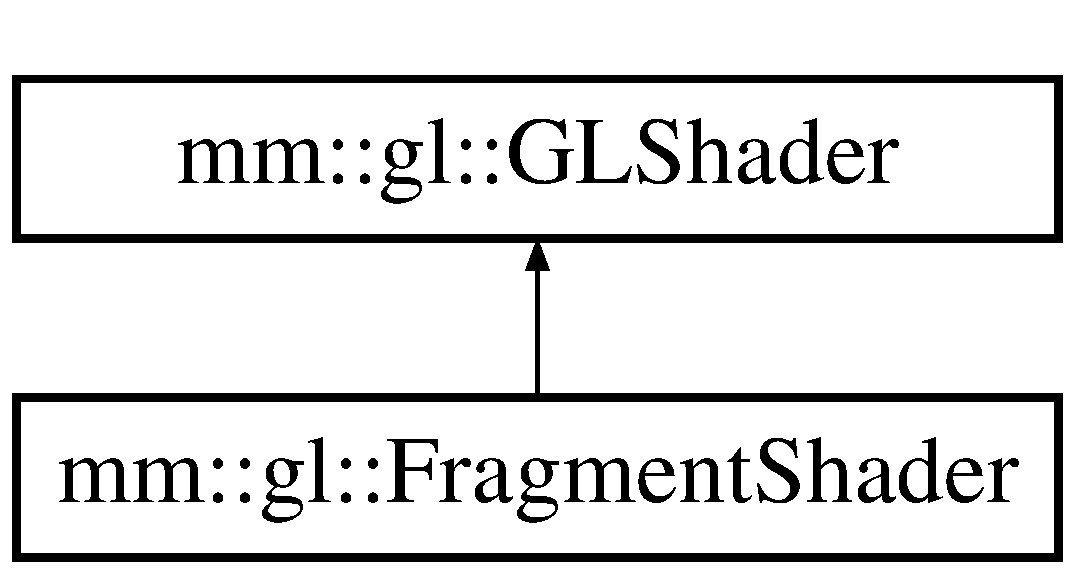
\includegraphics[height=2.000000cm]{classmm_1_1gl_1_1_fragment_shader}
\end{center}
\end{figure}
\subsection*{Public Member Functions}
\begin{DoxyCompactItemize}
\item 
\hypertarget{classmm_1_1gl_1_1_fragment_shader_a99eedc23f36c77fce19d68189f20a8d2}{}{\bfseries Fragment\+Shader} (const std\+::string \&filename)\label{classmm_1_1gl_1_1_fragment_shader_a99eedc23f36c77fce19d68189f20a8d2}

\end{DoxyCompactItemize}
\subsection*{Additional Inherited Members}


The documentation for this class was generated from the following files\+:\begin{DoxyCompactItemize}
\item 
src/core/mm\+\_\+opengl.\+h\item 
src/core/mm\+\_\+opengl.\+cc\end{DoxyCompactItemize}

\hypertarget{classmm_1_1_game_utils}{}\section{mm\+:\+:Game\+Utils Class Reference}
\label{classmm_1_1_game_utils}\index{mm\+::\+Game\+Utils@{mm\+::\+Game\+Utils}}


{\ttfamily \#include $<$mm\+\_\+utils.\+h$>$}

\subsection*{Static Public Member Functions}
\begin{DoxyCompactItemize}
\item 
\hypertarget{classmm_1_1_game_utils_a4118fb069fcca220219a341ef0ebc362}{}static int {\bfseries read\+Int} (const char $\ast$data)\label{classmm_1_1_game_utils_a4118fb069fcca220219a341ef0ebc362}

\item 
\hypertarget{classmm_1_1_game_utils_a783d8570e2dda319ba673e0092d1d540}{}static std\+::string {\bfseries write\+Int} (int data)\label{classmm_1_1_game_utils_a783d8570e2dda319ba673e0092d1d540}

\item 
static void \hyperlink{classmm_1_1_game_utils_a363d6db2c1f097e8142a4360bfcb4af5}{debug\+Bytes} (const B\+Y\+T\+E $\ast$data, uint size)
\item 
\hypertarget{classmm_1_1_game_utils_afaf0e91873157d243e8aa291565210c4}{}static void {\bfseries debug\+Bytes} (const std\+::string \&data, uint size)\label{classmm_1_1_game_utils_afaf0e91873157d243e8aa291565210c4}

\item 
\hypertarget{classmm_1_1_game_utils_a20607cbde377a9a9bb2df318d8ea4fab}{}static void {\bfseries debug\+Bytes} (const std\+::string \&data)\label{classmm_1_1_game_utils_a20607cbde377a9a9bb2df318d8ea4fab}

\item 
\hypertarget{classmm_1_1_game_utils_a9228b9b83fc986a616b55f7d20a76c42}{}static std\+::string {\bfseries to\+Hex} (uint n)\label{classmm_1_1_game_utils_a9228b9b83fc986a616b55f7d20a76c42}

\item 
\hypertarget{classmm_1_1_game_utils_a13d6a30776f7632a8a87469936493871}{}static std\+::string {\bfseries to\+S\+F} (uint n, uint size)\label{classmm_1_1_game_utils_a13d6a30776f7632a8a87469936493871}

\item 
\hypertarget{classmm_1_1_game_utils_a00c9d555eb5579317ca9e5d45bd2c548}{}static std\+::string {\bfseries to\+S\+F} (uint n)\label{classmm_1_1_game_utils_a00c9d555eb5579317ca9e5d45bd2c548}

\item 
\hypertarget{classmm_1_1_game_utils_aab9fe722279704cb7544a04a6027cccc}{}static std\+::string {\bfseries change\+Encoding} (const std\+::string \&source, const std\+::string \&from\+Code, const std\+::string \&to\+Code)\label{classmm_1_1_game_utils_aab9fe722279704cb7544a04a6027cccc}

\item 
\hypertarget{classmm_1_1_game_utils_ae6ee9cb4d479d5239ad1d843e1c9d0fd}{}static uint {\bfseries make\+I\+D} (uint \&id\+Index, uint mask=0x\+F\+F\+F\+F\+F\+F\+F\+F)\label{classmm_1_1_game_utils_ae6ee9cb4d479d5239ad1d843e1c9d0fd}

\item 
\hypertarget{classmm_1_1_game_utils_aed4dbd305d1dce87a586ba094a6d5cde}{}static long {\bfseries time\+Stamp} ()\label{classmm_1_1_game_utils_aed4dbd305d1dce87a586ba094a6d5cde}

\item 
\hypertarget{classmm_1_1_game_utils_aafda084db416548d59fac50342584169}{}static uint64 {\bfseries ms\+Time\+Stamp} ()\label{classmm_1_1_game_utils_aafda084db416548d59fac50342584169}

\item 
\hypertarget{classmm_1_1_game_utils_a7b22255b7f41daccf69e9ba4f0eae5cb}{}static std\+::string {\bfseries time\+String} (long t=0)\label{classmm_1_1_game_utils_a7b22255b7f41daccf69e9ba4f0eae5cb}

\item 
\hypertarget{classmm_1_1_game_utils_a52e35ff5c36fa9db64652a44b52369ba}{}static std\+::string {\bfseries ms\+Time\+String} (uint64 t=0)\label{classmm_1_1_game_utils_a52e35ff5c36fa9db64652a44b52369ba}

\item 
\hypertarget{classmm_1_1_game_utils_a03f45f460b5e9d6b833eaa60295f160e}{}static double {\bfseries distance} (int x1, int y1, int x2, int y2)\label{classmm_1_1_game_utils_a03f45f460b5e9d6b833eaa60295f160e}

\item 
\hypertarget{classmm_1_1_game_utils_a983731ec0aa94bb60acad4fb9cf1f12b}{}static double {\bfseries P2\+P\+Angle} (int x1, int y1, int x2, int y2)\label{classmm_1_1_game_utils_a983731ec0aa94bb60acad4fb9cf1f12b}

\item 
\hypertarget{classmm_1_1_game_utils_aa3dfc97cea897a49de5f4ec3adec34bd}{}static int {\bfseries distance\+X} (double distance, double angle)\label{classmm_1_1_game_utils_aa3dfc97cea897a49de5f4ec3adec34bd}

\item 
\hypertarget{classmm_1_1_game_utils_aafe13b84d91201e21e25daa57e6975e7}{}static int {\bfseries distance\+Y} (double distance, double angle)\label{classmm_1_1_game_utils_aafe13b84d91201e21e25daa57e6975e7}

\item 
\hypertarget{classmm_1_1_game_utils_ac114d8b06c290716b9910af6bcdc2ec5}{}static int {\bfseries angle28\+Dir} (double angle)\label{classmm_1_1_game_utils_ac114d8b06c290716b9910af6bcdc2ec5}

\item 
\hypertarget{classmm_1_1_game_utils_a14a03026aa4d0a6c54a066186456d55e}{}static int {\bfseries P2\+P28\+Dir} (int x1, int y1, int x2, int y2)\label{classmm_1_1_game_utils_a14a03026aa4d0a6c54a066186456d55e}

\end{DoxyCompactItemize}


\subsection{Detailed Description}
一些不好分类的公用方法 

\subsection{Member Function Documentation}
\hypertarget{classmm_1_1_game_utils_a363d6db2c1f097e8142a4360bfcb4af5}{}\index{mm\+::\+Game\+Utils@{mm\+::\+Game\+Utils}!debug\+Bytes@{debug\+Bytes}}
\index{debug\+Bytes@{debug\+Bytes}!mm\+::\+Game\+Utils@{mm\+::\+Game\+Utils}}
\subsubsection[{debug\+Bytes}]{\setlength{\rightskip}{0pt plus 5cm}void Game\+Utils\+::debug\+Bytes (
\begin{DoxyParamCaption}
\item[{const B\+Y\+T\+E $\ast$}]{data, }
\item[{uint}]{size}
\end{DoxyParamCaption}
)\hspace{0.3cm}{\ttfamily [static]}}\label{classmm_1_1_game_utils_a363d6db2c1f097e8142a4360bfcb4af5}
以二进制的方式显示一个字符串的信息 

The documentation for this class was generated from the following files\+:\begin{DoxyCompactItemize}
\item 
src/core/mm\+\_\+utils.\+h\item 
src/core/mm\+\_\+utils.\+cc\end{DoxyCompactItemize}

\hypertarget{classstd_1_1tr1_1_1gtest__internal_1_1_get}{}\section{std\+:\+:tr1\+:\+:gtest\+\_\+internal\+:\+:Get$<$ k $>$ Class Template Reference}
\label{classstd_1_1tr1_1_1gtest__internal_1_1_get}\index{std\+::tr1\+::gtest\+\_\+internal\+::\+Get$<$ k $>$@{std\+::tr1\+::gtest\+\_\+internal\+::\+Get$<$ k $>$}}


The documentation for this class was generated from the following file\+:\begin{DoxyCompactItemize}
\item 
deps/win32/debug/include/gtest/internal/gtest-\/tuple.\+h\end{DoxyCompactItemize}

\hypertarget{classstd_1_1tr1_1_1gtest__internal_1_1_get_3_010_01_4}{}\section{std\+:\+:tr1\+:\+:gtest\+\_\+internal\+:\+:Get$<$ 0 $>$ Class Template Reference}
\label{classstd_1_1tr1_1_1gtest__internal_1_1_get_3_010_01_4}\index{std\+::tr1\+::gtest\+\_\+internal\+::\+Get$<$ 0 $>$@{std\+::tr1\+::gtest\+\_\+internal\+::\+Get$<$ 0 $>$}}
\subsection*{Static Public Member Functions}
\begin{DoxyCompactItemize}
\item 
\hypertarget{classstd_1_1tr1_1_1gtest__internal_1_1_get_3_010_01_4_a74beca3869fddfe42ee608b7f4cacb96}{}{\footnotesize template$<$class Tuple $>$ }\\static {\bfseries G\+T\+E\+S\+T\+\_\+\+A\+D\+D\+\_\+\+R\+E\+F\+\_\+} (G\+T\+E\+S\+T\+\_\+\+T\+U\+P\+L\+E\+\_\+\+E\+L\+E\+M\+E\+N\+T\+\_\+(0, Tuple)) Field(Tuple \&t)\label{classstd_1_1tr1_1_1gtest__internal_1_1_get_3_010_01_4_a74beca3869fddfe42ee608b7f4cacb96}

\item 
\hypertarget{classstd_1_1tr1_1_1gtest__internal_1_1_get_3_010_01_4_a195b3853de45077f9a324c455f22d7e2}{}{\footnotesize template$<$class Tuple $>$ }\\static {\bfseries G\+T\+E\+S\+T\+\_\+\+B\+Y\+\_\+\+R\+E\+F\+\_\+} (G\+T\+E\+S\+T\+\_\+\+T\+U\+P\+L\+E\+\_\+\+E\+L\+E\+M\+E\+N\+T\+\_\+(0, Tuple)) Const\+Field(const Tuple \&t)\label{classstd_1_1tr1_1_1gtest__internal_1_1_get_3_010_01_4_a195b3853de45077f9a324c455f22d7e2}

\item 
\hypertarget{classstd_1_1tr1_1_1gtest__internal_1_1_get_3_010_01_4_a74beca3869fddfe42ee608b7f4cacb96}{}{\footnotesize template$<$class Tuple $>$ }\\static {\bfseries G\+T\+E\+S\+T\+\_\+\+A\+D\+D\+\_\+\+R\+E\+F\+\_\+} (G\+T\+E\+S\+T\+\_\+\+T\+U\+P\+L\+E\+\_\+\+E\+L\+E\+M\+E\+N\+T\+\_\+(0, Tuple)) Field(Tuple \&t)\label{classstd_1_1tr1_1_1gtest__internal_1_1_get_3_010_01_4_a74beca3869fddfe42ee608b7f4cacb96}

\item 
\hypertarget{classstd_1_1tr1_1_1gtest__internal_1_1_get_3_010_01_4_a195b3853de45077f9a324c455f22d7e2}{}{\footnotesize template$<$class Tuple $>$ }\\static {\bfseries G\+T\+E\+S\+T\+\_\+\+B\+Y\+\_\+\+R\+E\+F\+\_\+} (G\+T\+E\+S\+T\+\_\+\+T\+U\+P\+L\+E\+\_\+\+E\+L\+E\+M\+E\+N\+T\+\_\+(0, Tuple)) Const\+Field(const Tuple \&t)\label{classstd_1_1tr1_1_1gtest__internal_1_1_get_3_010_01_4_a195b3853de45077f9a324c455f22d7e2}

\end{DoxyCompactItemize}


The documentation for this class was generated from the following file\+:\begin{DoxyCompactItemize}
\item 
deps/win32/debug/include/gtest/internal/gtest-\/tuple.\+h\end{DoxyCompactItemize}

\hypertarget{classstd_1_1tr1_1_1gtest__internal_1_1_get_3_011_01_4}{}\section{std\+:\+:tr1\+:\+:gtest\+\_\+internal\+:\+:Get$<$ 1 $>$ Class Template Reference}
\label{classstd_1_1tr1_1_1gtest__internal_1_1_get_3_011_01_4}\index{std\+::tr1\+::gtest\+\_\+internal\+::\+Get$<$ 1 $>$@{std\+::tr1\+::gtest\+\_\+internal\+::\+Get$<$ 1 $>$}}
\subsection*{Static Public Member Functions}
\begin{DoxyCompactItemize}
\item 
\hypertarget{classstd_1_1tr1_1_1gtest__internal_1_1_get_3_011_01_4_a52b2f5d2bc283d76a3e8dede84dba154}{}{\footnotesize template$<$class Tuple $>$ }\\static {\bfseries G\+T\+E\+S\+T\+\_\+\+A\+D\+D\+\_\+\+R\+E\+F\+\_\+} (G\+T\+E\+S\+T\+\_\+\+T\+U\+P\+L\+E\+\_\+\+E\+L\+E\+M\+E\+N\+T\+\_\+(1, Tuple)) Field(Tuple \&t)\label{classstd_1_1tr1_1_1gtest__internal_1_1_get_3_011_01_4_a52b2f5d2bc283d76a3e8dede84dba154}

\item 
\hypertarget{classstd_1_1tr1_1_1gtest__internal_1_1_get_3_011_01_4_a481a2bf839c758408d46a1d0d41ff8f4}{}{\footnotesize template$<$class Tuple $>$ }\\static {\bfseries G\+T\+E\+S\+T\+\_\+\+B\+Y\+\_\+\+R\+E\+F\+\_\+} (G\+T\+E\+S\+T\+\_\+\+T\+U\+P\+L\+E\+\_\+\+E\+L\+E\+M\+E\+N\+T\+\_\+(1, Tuple)) Const\+Field(const Tuple \&t)\label{classstd_1_1tr1_1_1gtest__internal_1_1_get_3_011_01_4_a481a2bf839c758408d46a1d0d41ff8f4}

\item 
\hypertarget{classstd_1_1tr1_1_1gtest__internal_1_1_get_3_011_01_4_a52b2f5d2bc283d76a3e8dede84dba154}{}{\footnotesize template$<$class Tuple $>$ }\\static {\bfseries G\+T\+E\+S\+T\+\_\+\+A\+D\+D\+\_\+\+R\+E\+F\+\_\+} (G\+T\+E\+S\+T\+\_\+\+T\+U\+P\+L\+E\+\_\+\+E\+L\+E\+M\+E\+N\+T\+\_\+(1, Tuple)) Field(Tuple \&t)\label{classstd_1_1tr1_1_1gtest__internal_1_1_get_3_011_01_4_a52b2f5d2bc283d76a3e8dede84dba154}

\item 
\hypertarget{classstd_1_1tr1_1_1gtest__internal_1_1_get_3_011_01_4_a481a2bf839c758408d46a1d0d41ff8f4}{}{\footnotesize template$<$class Tuple $>$ }\\static {\bfseries G\+T\+E\+S\+T\+\_\+\+B\+Y\+\_\+\+R\+E\+F\+\_\+} (G\+T\+E\+S\+T\+\_\+\+T\+U\+P\+L\+E\+\_\+\+E\+L\+E\+M\+E\+N\+T\+\_\+(1, Tuple)) Const\+Field(const Tuple \&t)\label{classstd_1_1tr1_1_1gtest__internal_1_1_get_3_011_01_4_a481a2bf839c758408d46a1d0d41ff8f4}

\end{DoxyCompactItemize}


The documentation for this class was generated from the following file\+:\begin{DoxyCompactItemize}
\item 
deps/win32/debug/include/gtest/internal/gtest-\/tuple.\+h\end{DoxyCompactItemize}

\hypertarget{classstd_1_1tr1_1_1gtest__internal_1_1_get_3_012_01_4}{}\section{std\+:\+:tr1\+:\+:gtest\+\_\+internal\+:\+:Get$<$ 2 $>$ Class Template Reference}
\label{classstd_1_1tr1_1_1gtest__internal_1_1_get_3_012_01_4}\index{std\+::tr1\+::gtest\+\_\+internal\+::\+Get$<$ 2 $>$@{std\+::tr1\+::gtest\+\_\+internal\+::\+Get$<$ 2 $>$}}
\subsection*{Static Public Member Functions}
\begin{DoxyCompactItemize}
\item 
\hypertarget{classstd_1_1tr1_1_1gtest__internal_1_1_get_3_012_01_4_a8dfe7b5c1c915f10181e3fb5952ba6d8}{}{\footnotesize template$<$class Tuple $>$ }\\static {\bfseries G\+T\+E\+S\+T\+\_\+\+A\+D\+D\+\_\+\+R\+E\+F\+\_\+} (G\+T\+E\+S\+T\+\_\+\+T\+U\+P\+L\+E\+\_\+\+E\+L\+E\+M\+E\+N\+T\+\_\+(2, Tuple)) Field(Tuple \&t)\label{classstd_1_1tr1_1_1gtest__internal_1_1_get_3_012_01_4_a8dfe7b5c1c915f10181e3fb5952ba6d8}

\item 
\hypertarget{classstd_1_1tr1_1_1gtest__internal_1_1_get_3_012_01_4_a76127c9c03c1f0caa61fb87d4d756b5b}{}{\footnotesize template$<$class Tuple $>$ }\\static {\bfseries G\+T\+E\+S\+T\+\_\+\+B\+Y\+\_\+\+R\+E\+F\+\_\+} (G\+T\+E\+S\+T\+\_\+\+T\+U\+P\+L\+E\+\_\+\+E\+L\+E\+M\+E\+N\+T\+\_\+(2, Tuple)) Const\+Field(const Tuple \&t)\label{classstd_1_1tr1_1_1gtest__internal_1_1_get_3_012_01_4_a76127c9c03c1f0caa61fb87d4d756b5b}

\item 
\hypertarget{classstd_1_1tr1_1_1gtest__internal_1_1_get_3_012_01_4_a8dfe7b5c1c915f10181e3fb5952ba6d8}{}{\footnotesize template$<$class Tuple $>$ }\\static {\bfseries G\+T\+E\+S\+T\+\_\+\+A\+D\+D\+\_\+\+R\+E\+F\+\_\+} (G\+T\+E\+S\+T\+\_\+\+T\+U\+P\+L\+E\+\_\+\+E\+L\+E\+M\+E\+N\+T\+\_\+(2, Tuple)) Field(Tuple \&t)\label{classstd_1_1tr1_1_1gtest__internal_1_1_get_3_012_01_4_a8dfe7b5c1c915f10181e3fb5952ba6d8}

\item 
\hypertarget{classstd_1_1tr1_1_1gtest__internal_1_1_get_3_012_01_4_a76127c9c03c1f0caa61fb87d4d756b5b}{}{\footnotesize template$<$class Tuple $>$ }\\static {\bfseries G\+T\+E\+S\+T\+\_\+\+B\+Y\+\_\+\+R\+E\+F\+\_\+} (G\+T\+E\+S\+T\+\_\+\+T\+U\+P\+L\+E\+\_\+\+E\+L\+E\+M\+E\+N\+T\+\_\+(2, Tuple)) Const\+Field(const Tuple \&t)\label{classstd_1_1tr1_1_1gtest__internal_1_1_get_3_012_01_4_a76127c9c03c1f0caa61fb87d4d756b5b}

\end{DoxyCompactItemize}


The documentation for this class was generated from the following file\+:\begin{DoxyCompactItemize}
\item 
deps/win32/debug/include/gtest/internal/gtest-\/tuple.\+h\end{DoxyCompactItemize}

\hypertarget{classstd_1_1tr1_1_1gtest__internal_1_1_get_3_013_01_4}{}\section{std\+:\+:tr1\+:\+:gtest\+\_\+internal\+:\+:Get$<$ 3 $>$ Class Template Reference}
\label{classstd_1_1tr1_1_1gtest__internal_1_1_get_3_013_01_4}\index{std\+::tr1\+::gtest\+\_\+internal\+::\+Get$<$ 3 $>$@{std\+::tr1\+::gtest\+\_\+internal\+::\+Get$<$ 3 $>$}}
\subsection*{Static Public Member Functions}
\begin{DoxyCompactItemize}
\item 
\hypertarget{classstd_1_1tr1_1_1gtest__internal_1_1_get_3_013_01_4_aa2ebd71eca812f06bad0773a7e2f6788}{}{\footnotesize template$<$class Tuple $>$ }\\static {\bfseries G\+T\+E\+S\+T\+\_\+\+A\+D\+D\+\_\+\+R\+E\+F\+\_\+} (G\+T\+E\+S\+T\+\_\+\+T\+U\+P\+L\+E\+\_\+\+E\+L\+E\+M\+E\+N\+T\+\_\+(3, Tuple)) Field(Tuple \&t)\label{classstd_1_1tr1_1_1gtest__internal_1_1_get_3_013_01_4_aa2ebd71eca812f06bad0773a7e2f6788}

\item 
\hypertarget{classstd_1_1tr1_1_1gtest__internal_1_1_get_3_013_01_4_ab8c5283e6776308abc41aaad518a23c7}{}{\footnotesize template$<$class Tuple $>$ }\\static {\bfseries G\+T\+E\+S\+T\+\_\+\+B\+Y\+\_\+\+R\+E\+F\+\_\+} (G\+T\+E\+S\+T\+\_\+\+T\+U\+P\+L\+E\+\_\+\+E\+L\+E\+M\+E\+N\+T\+\_\+(3, Tuple)) Const\+Field(const Tuple \&t)\label{classstd_1_1tr1_1_1gtest__internal_1_1_get_3_013_01_4_ab8c5283e6776308abc41aaad518a23c7}

\item 
\hypertarget{classstd_1_1tr1_1_1gtest__internal_1_1_get_3_013_01_4_aa2ebd71eca812f06bad0773a7e2f6788}{}{\footnotesize template$<$class Tuple $>$ }\\static {\bfseries G\+T\+E\+S\+T\+\_\+\+A\+D\+D\+\_\+\+R\+E\+F\+\_\+} (G\+T\+E\+S\+T\+\_\+\+T\+U\+P\+L\+E\+\_\+\+E\+L\+E\+M\+E\+N\+T\+\_\+(3, Tuple)) Field(Tuple \&t)\label{classstd_1_1tr1_1_1gtest__internal_1_1_get_3_013_01_4_aa2ebd71eca812f06bad0773a7e2f6788}

\item 
\hypertarget{classstd_1_1tr1_1_1gtest__internal_1_1_get_3_013_01_4_ab8c5283e6776308abc41aaad518a23c7}{}{\footnotesize template$<$class Tuple $>$ }\\static {\bfseries G\+T\+E\+S\+T\+\_\+\+B\+Y\+\_\+\+R\+E\+F\+\_\+} (G\+T\+E\+S\+T\+\_\+\+T\+U\+P\+L\+E\+\_\+\+E\+L\+E\+M\+E\+N\+T\+\_\+(3, Tuple)) Const\+Field(const Tuple \&t)\label{classstd_1_1tr1_1_1gtest__internal_1_1_get_3_013_01_4_ab8c5283e6776308abc41aaad518a23c7}

\end{DoxyCompactItemize}


The documentation for this class was generated from the following file\+:\begin{DoxyCompactItemize}
\item 
deps/win32/debug/include/gtest/internal/gtest-\/tuple.\+h\end{DoxyCompactItemize}

\hypertarget{classstd_1_1tr1_1_1gtest__internal_1_1_get_3_014_01_4}{}\section{std\+:\+:tr1\+:\+:gtest\+\_\+internal\+:\+:Get$<$ 4 $>$ Class Template Reference}
\label{classstd_1_1tr1_1_1gtest__internal_1_1_get_3_014_01_4}\index{std\+::tr1\+::gtest\+\_\+internal\+::\+Get$<$ 4 $>$@{std\+::tr1\+::gtest\+\_\+internal\+::\+Get$<$ 4 $>$}}
\subsection*{Static Public Member Functions}
\begin{DoxyCompactItemize}
\item 
\hypertarget{classstd_1_1tr1_1_1gtest__internal_1_1_get_3_014_01_4_a5c7a91c681118bb7253e305f8ff42be4}{}{\footnotesize template$<$class Tuple $>$ }\\static {\bfseries G\+T\+E\+S\+T\+\_\+\+A\+D\+D\+\_\+\+R\+E\+F\+\_\+} (G\+T\+E\+S\+T\+\_\+\+T\+U\+P\+L\+E\+\_\+\+E\+L\+E\+M\+E\+N\+T\+\_\+(4, Tuple)) Field(Tuple \&t)\label{classstd_1_1tr1_1_1gtest__internal_1_1_get_3_014_01_4_a5c7a91c681118bb7253e305f8ff42be4}

\item 
\hypertarget{classstd_1_1tr1_1_1gtest__internal_1_1_get_3_014_01_4_a04794c398bbe81e4de0915b79da2166a}{}{\footnotesize template$<$class Tuple $>$ }\\static {\bfseries G\+T\+E\+S\+T\+\_\+\+B\+Y\+\_\+\+R\+E\+F\+\_\+} (G\+T\+E\+S\+T\+\_\+\+T\+U\+P\+L\+E\+\_\+\+E\+L\+E\+M\+E\+N\+T\+\_\+(4, Tuple)) Const\+Field(const Tuple \&t)\label{classstd_1_1tr1_1_1gtest__internal_1_1_get_3_014_01_4_a04794c398bbe81e4de0915b79da2166a}

\item 
\hypertarget{classstd_1_1tr1_1_1gtest__internal_1_1_get_3_014_01_4_a5c7a91c681118bb7253e305f8ff42be4}{}{\footnotesize template$<$class Tuple $>$ }\\static {\bfseries G\+T\+E\+S\+T\+\_\+\+A\+D\+D\+\_\+\+R\+E\+F\+\_\+} (G\+T\+E\+S\+T\+\_\+\+T\+U\+P\+L\+E\+\_\+\+E\+L\+E\+M\+E\+N\+T\+\_\+(4, Tuple)) Field(Tuple \&t)\label{classstd_1_1tr1_1_1gtest__internal_1_1_get_3_014_01_4_a5c7a91c681118bb7253e305f8ff42be4}

\item 
\hypertarget{classstd_1_1tr1_1_1gtest__internal_1_1_get_3_014_01_4_a04794c398bbe81e4de0915b79da2166a}{}{\footnotesize template$<$class Tuple $>$ }\\static {\bfseries G\+T\+E\+S\+T\+\_\+\+B\+Y\+\_\+\+R\+E\+F\+\_\+} (G\+T\+E\+S\+T\+\_\+\+T\+U\+P\+L\+E\+\_\+\+E\+L\+E\+M\+E\+N\+T\+\_\+(4, Tuple)) Const\+Field(const Tuple \&t)\label{classstd_1_1tr1_1_1gtest__internal_1_1_get_3_014_01_4_a04794c398bbe81e4de0915b79da2166a}

\end{DoxyCompactItemize}


The documentation for this class was generated from the following file\+:\begin{DoxyCompactItemize}
\item 
deps/win32/debug/include/gtest/internal/gtest-\/tuple.\+h\end{DoxyCompactItemize}

\hypertarget{classstd_1_1tr1_1_1gtest__internal_1_1_get_3_015_01_4}{}\section{std\+:\+:tr1\+:\+:gtest\+\_\+internal\+:\+:Get$<$ 5 $>$ Class Template Reference}
\label{classstd_1_1tr1_1_1gtest__internal_1_1_get_3_015_01_4}\index{std\+::tr1\+::gtest\+\_\+internal\+::\+Get$<$ 5 $>$@{std\+::tr1\+::gtest\+\_\+internal\+::\+Get$<$ 5 $>$}}
\subsection*{Static Public Member Functions}
\begin{DoxyCompactItemize}
\item 
\hypertarget{classstd_1_1tr1_1_1gtest__internal_1_1_get_3_015_01_4_a0a337088bab3f824f67d1607229fdcc2}{}{\footnotesize template$<$class Tuple $>$ }\\static {\bfseries G\+T\+E\+S\+T\+\_\+\+A\+D\+D\+\_\+\+R\+E\+F\+\_\+} (G\+T\+E\+S\+T\+\_\+\+T\+U\+P\+L\+E\+\_\+\+E\+L\+E\+M\+E\+N\+T\+\_\+(5, Tuple)) Field(Tuple \&t)\label{classstd_1_1tr1_1_1gtest__internal_1_1_get_3_015_01_4_a0a337088bab3f824f67d1607229fdcc2}

\item 
\hypertarget{classstd_1_1tr1_1_1gtest__internal_1_1_get_3_015_01_4_ae10fe16450db82d69b9a4d0b149ca75d}{}{\footnotesize template$<$class Tuple $>$ }\\static {\bfseries G\+T\+E\+S\+T\+\_\+\+B\+Y\+\_\+\+R\+E\+F\+\_\+} (G\+T\+E\+S\+T\+\_\+\+T\+U\+P\+L\+E\+\_\+\+E\+L\+E\+M\+E\+N\+T\+\_\+(5, Tuple)) Const\+Field(const Tuple \&t)\label{classstd_1_1tr1_1_1gtest__internal_1_1_get_3_015_01_4_ae10fe16450db82d69b9a4d0b149ca75d}

\item 
\hypertarget{classstd_1_1tr1_1_1gtest__internal_1_1_get_3_015_01_4_a0a337088bab3f824f67d1607229fdcc2}{}{\footnotesize template$<$class Tuple $>$ }\\static {\bfseries G\+T\+E\+S\+T\+\_\+\+A\+D\+D\+\_\+\+R\+E\+F\+\_\+} (G\+T\+E\+S\+T\+\_\+\+T\+U\+P\+L\+E\+\_\+\+E\+L\+E\+M\+E\+N\+T\+\_\+(5, Tuple)) Field(Tuple \&t)\label{classstd_1_1tr1_1_1gtest__internal_1_1_get_3_015_01_4_a0a337088bab3f824f67d1607229fdcc2}

\item 
\hypertarget{classstd_1_1tr1_1_1gtest__internal_1_1_get_3_015_01_4_ae10fe16450db82d69b9a4d0b149ca75d}{}{\footnotesize template$<$class Tuple $>$ }\\static {\bfseries G\+T\+E\+S\+T\+\_\+\+B\+Y\+\_\+\+R\+E\+F\+\_\+} (G\+T\+E\+S\+T\+\_\+\+T\+U\+P\+L\+E\+\_\+\+E\+L\+E\+M\+E\+N\+T\+\_\+(5, Tuple)) Const\+Field(const Tuple \&t)\label{classstd_1_1tr1_1_1gtest__internal_1_1_get_3_015_01_4_ae10fe16450db82d69b9a4d0b149ca75d}

\end{DoxyCompactItemize}


The documentation for this class was generated from the following file\+:\begin{DoxyCompactItemize}
\item 
deps/win32/debug/include/gtest/internal/gtest-\/tuple.\+h\end{DoxyCompactItemize}

\hypertarget{classstd_1_1tr1_1_1gtest__internal_1_1_get_3_016_01_4}{}\section{std\+:\+:tr1\+:\+:gtest\+\_\+internal\+:\+:Get$<$ 6 $>$ Class Template Reference}
\label{classstd_1_1tr1_1_1gtest__internal_1_1_get_3_016_01_4}\index{std\+::tr1\+::gtest\+\_\+internal\+::\+Get$<$ 6 $>$@{std\+::tr1\+::gtest\+\_\+internal\+::\+Get$<$ 6 $>$}}
\subsection*{Static Public Member Functions}
\begin{DoxyCompactItemize}
\item 
\hypertarget{classstd_1_1tr1_1_1gtest__internal_1_1_get_3_016_01_4_a28034152d066c8644fa55e9fc0e3a12d}{}{\footnotesize template$<$class Tuple $>$ }\\static {\bfseries G\+T\+E\+S\+T\+\_\+\+A\+D\+D\+\_\+\+R\+E\+F\+\_\+} (G\+T\+E\+S\+T\+\_\+\+T\+U\+P\+L\+E\+\_\+\+E\+L\+E\+M\+E\+N\+T\+\_\+(6, Tuple)) Field(Tuple \&t)\label{classstd_1_1tr1_1_1gtest__internal_1_1_get_3_016_01_4_a28034152d066c8644fa55e9fc0e3a12d}

\item 
\hypertarget{classstd_1_1tr1_1_1gtest__internal_1_1_get_3_016_01_4_a6e396b998757e0ab9b75db0c68a7c360}{}{\footnotesize template$<$class Tuple $>$ }\\static {\bfseries G\+T\+E\+S\+T\+\_\+\+B\+Y\+\_\+\+R\+E\+F\+\_\+} (G\+T\+E\+S\+T\+\_\+\+T\+U\+P\+L\+E\+\_\+\+E\+L\+E\+M\+E\+N\+T\+\_\+(6, Tuple)) Const\+Field(const Tuple \&t)\label{classstd_1_1tr1_1_1gtest__internal_1_1_get_3_016_01_4_a6e396b998757e0ab9b75db0c68a7c360}

\item 
\hypertarget{classstd_1_1tr1_1_1gtest__internal_1_1_get_3_016_01_4_a28034152d066c8644fa55e9fc0e3a12d}{}{\footnotesize template$<$class Tuple $>$ }\\static {\bfseries G\+T\+E\+S\+T\+\_\+\+A\+D\+D\+\_\+\+R\+E\+F\+\_\+} (G\+T\+E\+S\+T\+\_\+\+T\+U\+P\+L\+E\+\_\+\+E\+L\+E\+M\+E\+N\+T\+\_\+(6, Tuple)) Field(Tuple \&t)\label{classstd_1_1tr1_1_1gtest__internal_1_1_get_3_016_01_4_a28034152d066c8644fa55e9fc0e3a12d}

\item 
\hypertarget{classstd_1_1tr1_1_1gtest__internal_1_1_get_3_016_01_4_a6e396b998757e0ab9b75db0c68a7c360}{}{\footnotesize template$<$class Tuple $>$ }\\static {\bfseries G\+T\+E\+S\+T\+\_\+\+B\+Y\+\_\+\+R\+E\+F\+\_\+} (G\+T\+E\+S\+T\+\_\+\+T\+U\+P\+L\+E\+\_\+\+E\+L\+E\+M\+E\+N\+T\+\_\+(6, Tuple)) Const\+Field(const Tuple \&t)\label{classstd_1_1tr1_1_1gtest__internal_1_1_get_3_016_01_4_a6e396b998757e0ab9b75db0c68a7c360}

\end{DoxyCompactItemize}


The documentation for this class was generated from the following file\+:\begin{DoxyCompactItemize}
\item 
deps/win32/debug/include/gtest/internal/gtest-\/tuple.\+h\end{DoxyCompactItemize}

\hypertarget{classstd_1_1tr1_1_1gtest__internal_1_1_get_3_017_01_4}{}\section{std\+:\+:tr1\+:\+:gtest\+\_\+internal\+:\+:Get$<$ 7 $>$ Class Template Reference}
\label{classstd_1_1tr1_1_1gtest__internal_1_1_get_3_017_01_4}\index{std\+::tr1\+::gtest\+\_\+internal\+::\+Get$<$ 7 $>$@{std\+::tr1\+::gtest\+\_\+internal\+::\+Get$<$ 7 $>$}}
\subsection*{Static Public Member Functions}
\begin{DoxyCompactItemize}
\item 
\hypertarget{classstd_1_1tr1_1_1gtest__internal_1_1_get_3_017_01_4_ae1245f00b2ad610a130681b5bc81051c}{}{\footnotesize template$<$class Tuple $>$ }\\static {\bfseries G\+T\+E\+S\+T\+\_\+\+A\+D\+D\+\_\+\+R\+E\+F\+\_\+} (G\+T\+E\+S\+T\+\_\+\+T\+U\+P\+L\+E\+\_\+\+E\+L\+E\+M\+E\+N\+T\+\_\+(7, Tuple)) Field(Tuple \&t)\label{classstd_1_1tr1_1_1gtest__internal_1_1_get_3_017_01_4_ae1245f00b2ad610a130681b5bc81051c}

\item 
\hypertarget{classstd_1_1tr1_1_1gtest__internal_1_1_get_3_017_01_4_afb7bd56e0697304325cd157d11df4a7b}{}{\footnotesize template$<$class Tuple $>$ }\\static {\bfseries G\+T\+E\+S\+T\+\_\+\+B\+Y\+\_\+\+R\+E\+F\+\_\+} (G\+T\+E\+S\+T\+\_\+\+T\+U\+P\+L\+E\+\_\+\+E\+L\+E\+M\+E\+N\+T\+\_\+(7, Tuple)) Const\+Field(const Tuple \&t)\label{classstd_1_1tr1_1_1gtest__internal_1_1_get_3_017_01_4_afb7bd56e0697304325cd157d11df4a7b}

\item 
\hypertarget{classstd_1_1tr1_1_1gtest__internal_1_1_get_3_017_01_4_ae1245f00b2ad610a130681b5bc81051c}{}{\footnotesize template$<$class Tuple $>$ }\\static {\bfseries G\+T\+E\+S\+T\+\_\+\+A\+D\+D\+\_\+\+R\+E\+F\+\_\+} (G\+T\+E\+S\+T\+\_\+\+T\+U\+P\+L\+E\+\_\+\+E\+L\+E\+M\+E\+N\+T\+\_\+(7, Tuple)) Field(Tuple \&t)\label{classstd_1_1tr1_1_1gtest__internal_1_1_get_3_017_01_4_ae1245f00b2ad610a130681b5bc81051c}

\item 
\hypertarget{classstd_1_1tr1_1_1gtest__internal_1_1_get_3_017_01_4_afb7bd56e0697304325cd157d11df4a7b}{}{\footnotesize template$<$class Tuple $>$ }\\static {\bfseries G\+T\+E\+S\+T\+\_\+\+B\+Y\+\_\+\+R\+E\+F\+\_\+} (G\+T\+E\+S\+T\+\_\+\+T\+U\+P\+L\+E\+\_\+\+E\+L\+E\+M\+E\+N\+T\+\_\+(7, Tuple)) Const\+Field(const Tuple \&t)\label{classstd_1_1tr1_1_1gtest__internal_1_1_get_3_017_01_4_afb7bd56e0697304325cd157d11df4a7b}

\end{DoxyCompactItemize}


The documentation for this class was generated from the following file\+:\begin{DoxyCompactItemize}
\item 
deps/win32/debug/include/gtest/internal/gtest-\/tuple.\+h\end{DoxyCompactItemize}

\hypertarget{classstd_1_1tr1_1_1gtest__internal_1_1_get_3_018_01_4}{}\section{std\+:\+:tr1\+:\+:gtest\+\_\+internal\+:\+:Get$<$ 8 $>$ Class Template Reference}
\label{classstd_1_1tr1_1_1gtest__internal_1_1_get_3_018_01_4}\index{std\+::tr1\+::gtest\+\_\+internal\+::\+Get$<$ 8 $>$@{std\+::tr1\+::gtest\+\_\+internal\+::\+Get$<$ 8 $>$}}
\subsection*{Static Public Member Functions}
\begin{DoxyCompactItemize}
\item 
\hypertarget{classstd_1_1tr1_1_1gtest__internal_1_1_get_3_018_01_4_adf667300b7efed278f4ee3bf4d2edb85}{}{\footnotesize template$<$class Tuple $>$ }\\static {\bfseries G\+T\+E\+S\+T\+\_\+\+A\+D\+D\+\_\+\+R\+E\+F\+\_\+} (G\+T\+E\+S\+T\+\_\+\+T\+U\+P\+L\+E\+\_\+\+E\+L\+E\+M\+E\+N\+T\+\_\+(8, Tuple)) Field(Tuple \&t)\label{classstd_1_1tr1_1_1gtest__internal_1_1_get_3_018_01_4_adf667300b7efed278f4ee3bf4d2edb85}

\item 
\hypertarget{classstd_1_1tr1_1_1gtest__internal_1_1_get_3_018_01_4_ab9645513ad2f983157f4062c89e910e7}{}{\footnotesize template$<$class Tuple $>$ }\\static {\bfseries G\+T\+E\+S\+T\+\_\+\+B\+Y\+\_\+\+R\+E\+F\+\_\+} (G\+T\+E\+S\+T\+\_\+\+T\+U\+P\+L\+E\+\_\+\+E\+L\+E\+M\+E\+N\+T\+\_\+(8, Tuple)) Const\+Field(const Tuple \&t)\label{classstd_1_1tr1_1_1gtest__internal_1_1_get_3_018_01_4_ab9645513ad2f983157f4062c89e910e7}

\item 
\hypertarget{classstd_1_1tr1_1_1gtest__internal_1_1_get_3_018_01_4_adf667300b7efed278f4ee3bf4d2edb85}{}{\footnotesize template$<$class Tuple $>$ }\\static {\bfseries G\+T\+E\+S\+T\+\_\+\+A\+D\+D\+\_\+\+R\+E\+F\+\_\+} (G\+T\+E\+S\+T\+\_\+\+T\+U\+P\+L\+E\+\_\+\+E\+L\+E\+M\+E\+N\+T\+\_\+(8, Tuple)) Field(Tuple \&t)\label{classstd_1_1tr1_1_1gtest__internal_1_1_get_3_018_01_4_adf667300b7efed278f4ee3bf4d2edb85}

\item 
\hypertarget{classstd_1_1tr1_1_1gtest__internal_1_1_get_3_018_01_4_ab9645513ad2f983157f4062c89e910e7}{}{\footnotesize template$<$class Tuple $>$ }\\static {\bfseries G\+T\+E\+S\+T\+\_\+\+B\+Y\+\_\+\+R\+E\+F\+\_\+} (G\+T\+E\+S\+T\+\_\+\+T\+U\+P\+L\+E\+\_\+\+E\+L\+E\+M\+E\+N\+T\+\_\+(8, Tuple)) Const\+Field(const Tuple \&t)\label{classstd_1_1tr1_1_1gtest__internal_1_1_get_3_018_01_4_ab9645513ad2f983157f4062c89e910e7}

\end{DoxyCompactItemize}


The documentation for this class was generated from the following file\+:\begin{DoxyCompactItemize}
\item 
deps/win32/debug/include/gtest/internal/gtest-\/tuple.\+h\end{DoxyCompactItemize}

\hypertarget{classstd_1_1tr1_1_1gtest__internal_1_1_get_3_019_01_4}{}\section{std\+:\+:tr1\+:\+:gtest\+\_\+internal\+:\+:Get$<$ 9 $>$ Class Template Reference}
\label{classstd_1_1tr1_1_1gtest__internal_1_1_get_3_019_01_4}\index{std\+::tr1\+::gtest\+\_\+internal\+::\+Get$<$ 9 $>$@{std\+::tr1\+::gtest\+\_\+internal\+::\+Get$<$ 9 $>$}}
\subsection*{Static Public Member Functions}
\begin{DoxyCompactItemize}
\item 
\hypertarget{classstd_1_1tr1_1_1gtest__internal_1_1_get_3_019_01_4_add31197dfdb381d265e221ed62129f45}{}{\footnotesize template$<$class Tuple $>$ }\\static {\bfseries G\+T\+E\+S\+T\+\_\+\+A\+D\+D\+\_\+\+R\+E\+F\+\_\+} (G\+T\+E\+S\+T\+\_\+\+T\+U\+P\+L\+E\+\_\+\+E\+L\+E\+M\+E\+N\+T\+\_\+(9, Tuple)) Field(Tuple \&t)\label{classstd_1_1tr1_1_1gtest__internal_1_1_get_3_019_01_4_add31197dfdb381d265e221ed62129f45}

\item 
\hypertarget{classstd_1_1tr1_1_1gtest__internal_1_1_get_3_019_01_4_a5205e8da729e2bee446f5be0c65390af}{}{\footnotesize template$<$class Tuple $>$ }\\static {\bfseries G\+T\+E\+S\+T\+\_\+\+B\+Y\+\_\+\+R\+E\+F\+\_\+} (G\+T\+E\+S\+T\+\_\+\+T\+U\+P\+L\+E\+\_\+\+E\+L\+E\+M\+E\+N\+T\+\_\+(9, Tuple)) Const\+Field(const Tuple \&t)\label{classstd_1_1tr1_1_1gtest__internal_1_1_get_3_019_01_4_a5205e8da729e2bee446f5be0c65390af}

\item 
\hypertarget{classstd_1_1tr1_1_1gtest__internal_1_1_get_3_019_01_4_add31197dfdb381d265e221ed62129f45}{}{\footnotesize template$<$class Tuple $>$ }\\static {\bfseries G\+T\+E\+S\+T\+\_\+\+A\+D\+D\+\_\+\+R\+E\+F\+\_\+} (G\+T\+E\+S\+T\+\_\+\+T\+U\+P\+L\+E\+\_\+\+E\+L\+E\+M\+E\+N\+T\+\_\+(9, Tuple)) Field(Tuple \&t)\label{classstd_1_1tr1_1_1gtest__internal_1_1_get_3_019_01_4_add31197dfdb381d265e221ed62129f45}

\item 
\hypertarget{classstd_1_1tr1_1_1gtest__internal_1_1_get_3_019_01_4_a5205e8da729e2bee446f5be0c65390af}{}{\footnotesize template$<$class Tuple $>$ }\\static {\bfseries G\+T\+E\+S\+T\+\_\+\+B\+Y\+\_\+\+R\+E\+F\+\_\+} (G\+T\+E\+S\+T\+\_\+\+T\+U\+P\+L\+E\+\_\+\+E\+L\+E\+M\+E\+N\+T\+\_\+(9, Tuple)) Const\+Field(const Tuple \&t)\label{classstd_1_1tr1_1_1gtest__internal_1_1_get_3_019_01_4_a5205e8da729e2bee446f5be0c65390af}

\end{DoxyCompactItemize}


The documentation for this class was generated from the following file\+:\begin{DoxyCompactItemize}
\item 
deps/win32/debug/include/gtest/internal/gtest-\/tuple.\+h\end{DoxyCompactItemize}

\hypertarget{classmm_1_1gl_1_1_g_l_program}{}\section{mm\+:\+:gl\+:\+:G\+L\+Program Class Reference}
\label{classmm_1_1gl_1_1_g_l_program}\index{mm\+::gl\+::\+G\+L\+Program@{mm\+::gl\+::\+G\+L\+Program}}
Inheritance diagram for mm\+:\+:gl\+:\+:G\+L\+Program\+:\begin{figure}[H]
\begin{center}
\leavevmode
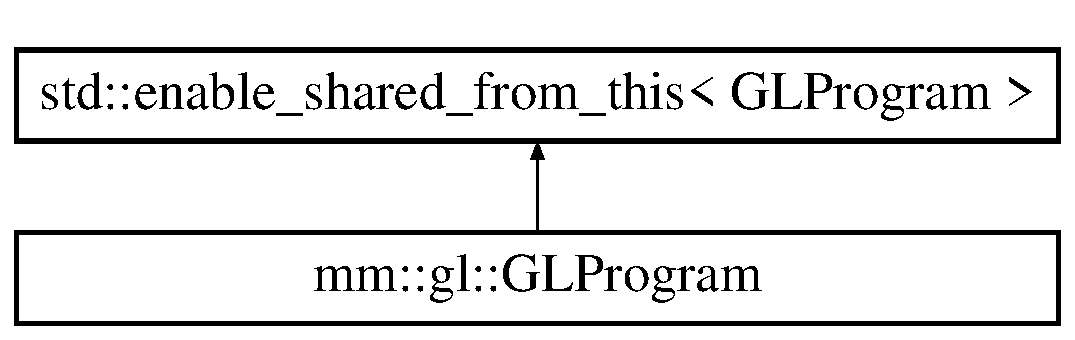
\includegraphics[height=2.000000cm]{classmm_1_1gl_1_1_g_l_program}
\end{center}
\end{figure}
\subsection*{Public Member Functions}
\begin{DoxyCompactItemize}
\item 
\hypertarget{classmm_1_1gl_1_1_g_l_program_ae8619a76f9e2004447a0cee8b5349994}{}void {\bfseries attach\+Shader} (P\+T\+R$<$ \hyperlink{classmm_1_1gl_1_1_g_l_shader}{G\+L\+Shader} $>$ shader)\label{classmm_1_1gl_1_1_g_l_program_ae8619a76f9e2004447a0cee8b5349994}

\item 
\hypertarget{classmm_1_1gl_1_1_g_l_program_a07aecd22ad9833f74c3f9a2493a0dff9}{}void {\bfseries use} ()\label{classmm_1_1gl_1_1_g_l_program_a07aecd22ad9833f74c3f9a2493a0dff9}

\end{DoxyCompactItemize}
\subsection*{Public Attributes}
\begin{DoxyCompactItemize}
\item 
\hypertarget{classmm_1_1gl_1_1_g_l_program_a85f9c487f1c83f67db4ba3a9a20c3e7e}{}G\+Luint {\bfseries handler}\label{classmm_1_1gl_1_1_g_l_program_a85f9c487f1c83f67db4ba3a9a20c3e7e}

\item 
\hypertarget{classmm_1_1gl_1_1_g_l_program_a2df2c466433f3536642dd910a54cbb32}{}bool {\bfseries is\+Compiled}\label{classmm_1_1gl_1_1_g_l_program_a2df2c466433f3536642dd910a54cbb32}

\item 
\hypertarget{classmm_1_1gl_1_1_g_l_program_aee49d710f8d8159942c6074776d16c1e}{}std\+::vector$<$ P\+T\+R$<$ \hyperlink{classmm_1_1gl_1_1_g_l_shader}{G\+L\+Shader} $>$ $>$ {\bfseries shaders}\label{classmm_1_1gl_1_1_g_l_program_aee49d710f8d8159942c6074776d16c1e}

\end{DoxyCompactItemize}


The documentation for this class was generated from the following files\+:\begin{DoxyCompactItemize}
\item 
src/core/mm\+\_\+opengl.\+h\item 
src/core/mm\+\_\+opengl.\+cc\end{DoxyCompactItemize}

\hypertarget{classmm_1_1gl_1_1_g_l_shader}{}\section{mm\+:\+:gl\+:\+:G\+L\+Shader Class Reference}
\label{classmm_1_1gl_1_1_g_l_shader}\index{mm\+::gl\+::\+G\+L\+Shader@{mm\+::gl\+::\+G\+L\+Shader}}
Inheritance diagram for mm\+:\+:gl\+:\+:G\+L\+Shader\+:\begin{figure}[H]
\begin{center}
\leavevmode
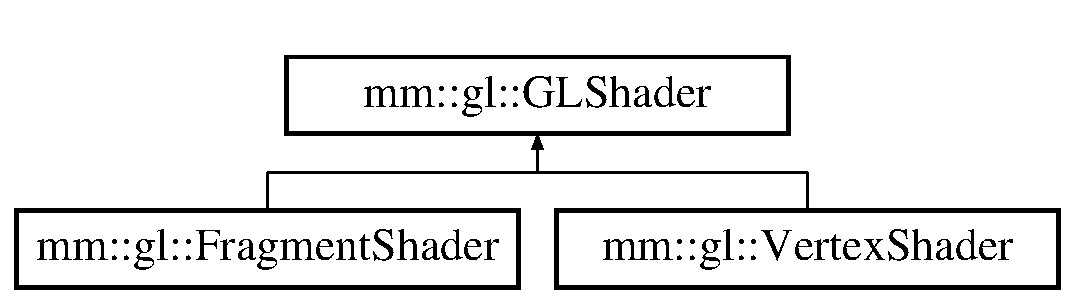
\includegraphics[height=2.000000cm]{classmm_1_1gl_1_1_g_l_shader}
\end{center}
\end{figure}
\subsection*{Public Member Functions}
\begin{DoxyCompactItemize}
\item 
\hypertarget{classmm_1_1gl_1_1_g_l_shader_a501cdad1fd1ce401dd40e87948b77d0d}{}{\bfseries G\+L\+Shader} (G\+Lenum type, const std\+::string \&filename)\label{classmm_1_1gl_1_1_g_l_shader_a501cdad1fd1ce401dd40e87948b77d0d}

\end{DoxyCompactItemize}
\subsection*{Public Attributes}
\begin{DoxyCompactItemize}
\item 
\hypertarget{classmm_1_1gl_1_1_g_l_shader_a99006821270e31a175bdfdb64f8f4217}{}G\+Lenum {\bfseries type}\label{classmm_1_1gl_1_1_g_l_shader_a99006821270e31a175bdfdb64f8f4217}

\item 
\hypertarget{classmm_1_1gl_1_1_g_l_shader_a33a3daec2995fd4f5df49d3d439da9fc}{}G\+Luint {\bfseries handler}\label{classmm_1_1gl_1_1_g_l_shader_a33a3daec2995fd4f5df49d3d439da9fc}

\item 
\hypertarget{classmm_1_1gl_1_1_g_l_shader_a0603b8f2a31d170f53328a547cdd1bec}{}std\+::string {\bfseries filename}\label{classmm_1_1gl_1_1_g_l_shader_a0603b8f2a31d170f53328a547cdd1bec}

\item 
\hypertarget{classmm_1_1gl_1_1_g_l_shader_af4f25142b975eb2e1512738e343939c9}{}std\+::string {\bfseries text}\label{classmm_1_1gl_1_1_g_l_shader_af4f25142b975eb2e1512738e343939c9}

\end{DoxyCompactItemize}
\subsection*{Protected Member Functions}
\begin{DoxyCompactItemize}
\item 
\hypertarget{classmm_1_1gl_1_1_g_l_shader_af07be10ef002cad67dc9eee60563e036}{}virtual void {\bfseries compile} ()\label{classmm_1_1gl_1_1_g_l_shader_af07be10ef002cad67dc9eee60563e036}

\end{DoxyCompactItemize}


The documentation for this class was generated from the following files\+:\begin{DoxyCompactItemize}
\item 
src/core/mm\+\_\+opengl.\+h\item 
src/core/mm\+\_\+opengl.\+cc\end{DoxyCompactItemize}

\hypertarget{struct_g_l_x_buffer_clobber_event_s_g_i_x}{}\section{G\+L\+X\+Buffer\+Clobber\+Event\+S\+G\+I\+X Struct Reference}
\label{struct_g_l_x_buffer_clobber_event_s_g_i_x}\index{G\+L\+X\+Buffer\+Clobber\+Event\+S\+G\+I\+X@{G\+L\+X\+Buffer\+Clobber\+Event\+S\+G\+I\+X}}
\subsection*{Public Attributes}
\begin{DoxyCompactItemize}
\item 
\hypertarget{struct_g_l_x_buffer_clobber_event_s_g_i_x_a36e3e8a5feea664623ea43d0f273b63a}{}int {\bfseries type}\label{struct_g_l_x_buffer_clobber_event_s_g_i_x_a36e3e8a5feea664623ea43d0f273b63a}

\item 
\hypertarget{struct_g_l_x_buffer_clobber_event_s_g_i_x_ac295e3276a7986eeae4d6a2a28c7e0b7}{}unsigned long {\bfseries serial}\label{struct_g_l_x_buffer_clobber_event_s_g_i_x_ac295e3276a7986eeae4d6a2a28c7e0b7}

\item 
\hypertarget{struct_g_l_x_buffer_clobber_event_s_g_i_x_af43bf0edbe40a74ef58dfb546a75118b}{}Bool {\bfseries send\+\_\+event}\label{struct_g_l_x_buffer_clobber_event_s_g_i_x_af43bf0edbe40a74ef58dfb546a75118b}

\item 
\hypertarget{struct_g_l_x_buffer_clobber_event_s_g_i_x_afef060d81026da75c846727f4a3de9d4}{}Display $\ast$ {\bfseries display}\label{struct_g_l_x_buffer_clobber_event_s_g_i_x_afef060d81026da75c846727f4a3de9d4}

\item 
\hypertarget{struct_g_l_x_buffer_clobber_event_s_g_i_x_a9c45674193ed80a79261c3b7518ee04f}{}G\+L\+X\+Drawable {\bfseries drawable}\label{struct_g_l_x_buffer_clobber_event_s_g_i_x_a9c45674193ed80a79261c3b7518ee04f}

\item 
\hypertarget{struct_g_l_x_buffer_clobber_event_s_g_i_x_a0b405123f1d6528f1f4dfa7ff92bde9b}{}int {\bfseries event\+\_\+type}\label{struct_g_l_x_buffer_clobber_event_s_g_i_x_a0b405123f1d6528f1f4dfa7ff92bde9b}

\item 
\hypertarget{struct_g_l_x_buffer_clobber_event_s_g_i_x_a25c31e8cbec0919f74a1e93ae74175b1}{}int {\bfseries draw\+\_\+type}\label{struct_g_l_x_buffer_clobber_event_s_g_i_x_a25c31e8cbec0919f74a1e93ae74175b1}

\item 
\hypertarget{struct_g_l_x_buffer_clobber_event_s_g_i_x_a74b4ad1ad3cac011001151411f621da1}{}unsigned int {\bfseries mask}\label{struct_g_l_x_buffer_clobber_event_s_g_i_x_a74b4ad1ad3cac011001151411f621da1}

\item 
\hypertarget{struct_g_l_x_buffer_clobber_event_s_g_i_x_a5118d48c3c8d5253d39922b5014b52ff}{}int {\bfseries x}\label{struct_g_l_x_buffer_clobber_event_s_g_i_x_a5118d48c3c8d5253d39922b5014b52ff}

\item 
\hypertarget{struct_g_l_x_buffer_clobber_event_s_g_i_x_aef21efa11558a5b67861f96471c56003}{}int {\bfseries y}\label{struct_g_l_x_buffer_clobber_event_s_g_i_x_aef21efa11558a5b67861f96471c56003}

\item 
\hypertarget{struct_g_l_x_buffer_clobber_event_s_g_i_x_adad23535733161528427584a42bfc6eb}{}int {\bfseries width}\label{struct_g_l_x_buffer_clobber_event_s_g_i_x_adad23535733161528427584a42bfc6eb}

\item 
\hypertarget{struct_g_l_x_buffer_clobber_event_s_g_i_x_a7838dbabb76c22aa8241310a3f2363ea}{}int {\bfseries height}\label{struct_g_l_x_buffer_clobber_event_s_g_i_x_a7838dbabb76c22aa8241310a3f2363ea}

\item 
\hypertarget{struct_g_l_x_buffer_clobber_event_s_g_i_x_ad8f4f0aae058e0a1ff542679823e37a9}{}int {\bfseries count}\label{struct_g_l_x_buffer_clobber_event_s_g_i_x_ad8f4f0aae058e0a1ff542679823e37a9}

\end{DoxyCompactItemize}


The documentation for this struct was generated from the following file\+:\begin{DoxyCompactItemize}
\item 
deps/win32/debug/include/\+G\+L/glxew.\+h\end{DoxyCompactItemize}

\hypertarget{struct_g_l_x_hyperpipe_config_s_g_i_x}{}\section{G\+L\+X\+Hyperpipe\+Config\+S\+G\+I\+X Struct Reference}
\label{struct_g_l_x_hyperpipe_config_s_g_i_x}\index{G\+L\+X\+Hyperpipe\+Config\+S\+G\+I\+X@{G\+L\+X\+Hyperpipe\+Config\+S\+G\+I\+X}}
\subsection*{Public Attributes}
\begin{DoxyCompactItemize}
\item 
\hypertarget{struct_g_l_x_hyperpipe_config_s_g_i_x_a9e3748f92005cac81cb44d4c67acccb8}{}char {\bfseries pipe\+Name} \mbox{[}G\+L\+X\+\_\+\+H\+Y\+P\+E\+R\+P\+I\+P\+E\+\_\+\+P\+I\+P\+E\+\_\+\+N\+A\+M\+E\+\_\+\+L\+E\+N\+G\+T\+H\+\_\+\+S\+G\+I\+X\mbox{]}\label{struct_g_l_x_hyperpipe_config_s_g_i_x_a9e3748f92005cac81cb44d4c67acccb8}

\item 
\hypertarget{struct_g_l_x_hyperpipe_config_s_g_i_x_abc812d8796ba89d5de4e33b3532d8335}{}int {\bfseries channel}\label{struct_g_l_x_hyperpipe_config_s_g_i_x_abc812d8796ba89d5de4e33b3532d8335}

\item 
\hypertarget{struct_g_l_x_hyperpipe_config_s_g_i_x_a093cfaaec305531f66e1120929b5b01b}{}unsigned int {\bfseries participation\+Type}\label{struct_g_l_x_hyperpipe_config_s_g_i_x_a093cfaaec305531f66e1120929b5b01b}

\item 
\hypertarget{struct_g_l_x_hyperpipe_config_s_g_i_x_afe9288e75dc1ae5e0f33eff978d7024d}{}int {\bfseries time\+Slice}\label{struct_g_l_x_hyperpipe_config_s_g_i_x_afe9288e75dc1ae5e0f33eff978d7024d}

\end{DoxyCompactItemize}


The documentation for this struct was generated from the following file\+:\begin{DoxyCompactItemize}
\item 
deps/win32/debug/include/\+G\+L/glxew.\+h\end{DoxyCompactItemize}

\hypertarget{struct_g_l_x_hyperpipe_network_s_g_i_x}{}\section{G\+L\+X\+Hyperpipe\+Network\+S\+G\+I\+X Struct Reference}
\label{struct_g_l_x_hyperpipe_network_s_g_i_x}\index{G\+L\+X\+Hyperpipe\+Network\+S\+G\+I\+X@{G\+L\+X\+Hyperpipe\+Network\+S\+G\+I\+X}}
\subsection*{Public Attributes}
\begin{DoxyCompactItemize}
\item 
\hypertarget{struct_g_l_x_hyperpipe_network_s_g_i_x_a6338b9717fa895aec16b932f2ef693ed}{}char {\bfseries pipe\+Name} \mbox{[}G\+L\+X\+\_\+\+H\+Y\+P\+E\+R\+P\+I\+P\+E\+\_\+\+P\+I\+P\+E\+\_\+\+N\+A\+M\+E\+\_\+\+L\+E\+N\+G\+T\+H\+\_\+\+S\+G\+I\+X\mbox{]}\label{struct_g_l_x_hyperpipe_network_s_g_i_x_a6338b9717fa895aec16b932f2ef693ed}

\item 
\hypertarget{struct_g_l_x_hyperpipe_network_s_g_i_x_a81393053988b32fadb0b21615024add1}{}int {\bfseries network\+Id}\label{struct_g_l_x_hyperpipe_network_s_g_i_x_a81393053988b32fadb0b21615024add1}

\end{DoxyCompactItemize}


The documentation for this struct was generated from the following file\+:\begin{DoxyCompactItemize}
\item 
deps/win32/debug/include/\+G\+L/glxew.\+h\end{DoxyCompactItemize}

\hypertarget{struct_g_l_x_pbuffer_clobber_event}{}\section{G\+L\+X\+Pbuffer\+Clobber\+Event Struct Reference}
\label{struct_g_l_x_pbuffer_clobber_event}\index{G\+L\+X\+Pbuffer\+Clobber\+Event@{G\+L\+X\+Pbuffer\+Clobber\+Event}}
\subsection*{Public Attributes}
\begin{DoxyCompactItemize}
\item 
\hypertarget{struct_g_l_x_pbuffer_clobber_event_a30d7162d8d77246b01f5e610cda4da68}{}int {\bfseries event\+\_\+type}\label{struct_g_l_x_pbuffer_clobber_event_a30d7162d8d77246b01f5e610cda4da68}

\item 
\hypertarget{struct_g_l_x_pbuffer_clobber_event_a243f92b79d3cfbde73eab02815be2320}{}int {\bfseries draw\+\_\+type}\label{struct_g_l_x_pbuffer_clobber_event_a243f92b79d3cfbde73eab02815be2320}

\item 
\hypertarget{struct_g_l_x_pbuffer_clobber_event_a6390b2875ae06a4cb827d2b4c321eda3}{}unsigned long {\bfseries serial}\label{struct_g_l_x_pbuffer_clobber_event_a6390b2875ae06a4cb827d2b4c321eda3}

\item 
\hypertarget{struct_g_l_x_pbuffer_clobber_event_aa51969e67e4ad6095bda26ca64fe8ba6}{}Bool {\bfseries send\+\_\+event}\label{struct_g_l_x_pbuffer_clobber_event_aa51969e67e4ad6095bda26ca64fe8ba6}

\item 
\hypertarget{struct_g_l_x_pbuffer_clobber_event_aeb49bb93cc59448e75d66170a39596d1}{}Display $\ast$ {\bfseries display}\label{struct_g_l_x_pbuffer_clobber_event_aeb49bb93cc59448e75d66170a39596d1}

\item 
\hypertarget{struct_g_l_x_pbuffer_clobber_event_a388908b766e35205c1a461ea8b60439f}{}G\+L\+X\+Drawable {\bfseries drawable}\label{struct_g_l_x_pbuffer_clobber_event_a388908b766e35205c1a461ea8b60439f}

\item 
\hypertarget{struct_g_l_x_pbuffer_clobber_event_aff4c23d00f6dad98427f8d32a5f10580}{}unsigned int {\bfseries buffer\+\_\+mask}\label{struct_g_l_x_pbuffer_clobber_event_aff4c23d00f6dad98427f8d32a5f10580}

\item 
\hypertarget{struct_g_l_x_pbuffer_clobber_event_a13193b6e7e3e52b15f754fe91403b7ec}{}unsigned int {\bfseries aux\+\_\+buffer}\label{struct_g_l_x_pbuffer_clobber_event_a13193b6e7e3e52b15f754fe91403b7ec}

\item 
\hypertarget{struct_g_l_x_pbuffer_clobber_event_a8f0a7162a033c89ee94ce535580dbc32}{}int {\bfseries x}\label{struct_g_l_x_pbuffer_clobber_event_a8f0a7162a033c89ee94ce535580dbc32}

\item 
\hypertarget{struct_g_l_x_pbuffer_clobber_event_a69eb7ac60d36ac3ec4550ac206cfc61f}{}int {\bfseries y}\label{struct_g_l_x_pbuffer_clobber_event_a69eb7ac60d36ac3ec4550ac206cfc61f}

\item 
\hypertarget{struct_g_l_x_pbuffer_clobber_event_aaca375fecb872c73c60cd5d0bfc7c7a5}{}int {\bfseries width}\label{struct_g_l_x_pbuffer_clobber_event_aaca375fecb872c73c60cd5d0bfc7c7a5}

\item 
\hypertarget{struct_g_l_x_pbuffer_clobber_event_aed4e539c896bdad15217bf92c28f8520}{}int {\bfseries height}\label{struct_g_l_x_pbuffer_clobber_event_aed4e539c896bdad15217bf92c28f8520}

\item 
\hypertarget{struct_g_l_x_pbuffer_clobber_event_a61e9f6b31738464dca67f909fcacd298}{}int {\bfseries count}\label{struct_g_l_x_pbuffer_clobber_event_a61e9f6b31738464dca67f909fcacd298}

\end{DoxyCompactItemize}


The documentation for this struct was generated from the following file\+:\begin{DoxyCompactItemize}
\item 
deps/win32/debug/include/\+G\+L/glxew.\+h\end{DoxyCompactItemize}

\hypertarget{struct_g_l_x_pipe_rect}{}\section{G\+L\+X\+Pipe\+Rect Struct Reference}
\label{struct_g_l_x_pipe_rect}\index{G\+L\+X\+Pipe\+Rect@{G\+L\+X\+Pipe\+Rect}}
\subsection*{Public Attributes}
\begin{DoxyCompactItemize}
\item 
\hypertarget{struct_g_l_x_pipe_rect_aa4c4f60e9647705ddefa10f95a37cb79}{}char {\bfseries pipe\+Name} \mbox{[}G\+L\+X\+\_\+\+H\+Y\+P\+E\+R\+P\+I\+P\+E\+\_\+\+P\+I\+P\+E\+\_\+\+N\+A\+M\+E\+\_\+\+L\+E\+N\+G\+T\+H\+\_\+\+S\+G\+I\+X\mbox{]}\label{struct_g_l_x_pipe_rect_aa4c4f60e9647705ddefa10f95a37cb79}

\item 
\hypertarget{struct_g_l_x_pipe_rect_a9df2313c01f75d149e64f2ff467bc266}{}int {\bfseries src\+X\+Origin}\label{struct_g_l_x_pipe_rect_a9df2313c01f75d149e64f2ff467bc266}

\item 
\hypertarget{struct_g_l_x_pipe_rect_a1f7316dff7050ab2ce9d3d37f8c5450e}{}int {\bfseries src\+Y\+Origin}\label{struct_g_l_x_pipe_rect_a1f7316dff7050ab2ce9d3d37f8c5450e}

\item 
\hypertarget{struct_g_l_x_pipe_rect_a2c6c180a4dabb71076366e06a1c7d0ef}{}int {\bfseries src\+Width}\label{struct_g_l_x_pipe_rect_a2c6c180a4dabb71076366e06a1c7d0ef}

\item 
\hypertarget{struct_g_l_x_pipe_rect_a35632524bce6bffa05f284a9b1c1b8ff}{}int {\bfseries src\+Height}\label{struct_g_l_x_pipe_rect_a35632524bce6bffa05f284a9b1c1b8ff}

\item 
\hypertarget{struct_g_l_x_pipe_rect_a8b7b941894ad3420326d7e9fa885bb71}{}int {\bfseries dest\+X\+Origin}\label{struct_g_l_x_pipe_rect_a8b7b941894ad3420326d7e9fa885bb71}

\item 
\hypertarget{struct_g_l_x_pipe_rect_aef7766b02ef07c20a11e89da5878b469}{}int {\bfseries dest\+Y\+Origin}\label{struct_g_l_x_pipe_rect_aef7766b02ef07c20a11e89da5878b469}

\item 
\hypertarget{struct_g_l_x_pipe_rect_a3c07991d2a8fb6e973eae834650b3dad}{}int {\bfseries dest\+Width}\label{struct_g_l_x_pipe_rect_a3c07991d2a8fb6e973eae834650b3dad}

\item 
\hypertarget{struct_g_l_x_pipe_rect_a858b0ea6642e451495aff35cfefbd083}{}int {\bfseries dest\+Height}\label{struct_g_l_x_pipe_rect_a858b0ea6642e451495aff35cfefbd083}

\end{DoxyCompactItemize}


The documentation for this struct was generated from the following file\+:\begin{DoxyCompactItemize}
\item 
deps/win32/debug/include/\+G\+L/glxew.\+h\end{DoxyCompactItemize}

\hypertarget{struct_g_l_x_pipe_rect_limits}{}\section{G\+L\+X\+Pipe\+Rect\+Limits Struct Reference}
\label{struct_g_l_x_pipe_rect_limits}\index{G\+L\+X\+Pipe\+Rect\+Limits@{G\+L\+X\+Pipe\+Rect\+Limits}}
\subsection*{Public Attributes}
\begin{DoxyCompactItemize}
\item 
\hypertarget{struct_g_l_x_pipe_rect_limits_ae78b4b6656101bc841946733a5b6e5ce}{}char {\bfseries pipe\+Name} \mbox{[}G\+L\+X\+\_\+\+H\+Y\+P\+E\+R\+P\+I\+P\+E\+\_\+\+P\+I\+P\+E\+\_\+\+N\+A\+M\+E\+\_\+\+L\+E\+N\+G\+T\+H\+\_\+\+S\+G\+I\+X\mbox{]}\label{struct_g_l_x_pipe_rect_limits_ae78b4b6656101bc841946733a5b6e5ce}

\item 
\hypertarget{struct_g_l_x_pipe_rect_limits_a3e5a965059d9f5d2ca42acd35af5bb9b}{}int {\bfseries X\+Origin}\label{struct_g_l_x_pipe_rect_limits_a3e5a965059d9f5d2ca42acd35af5bb9b}

\item 
\hypertarget{struct_g_l_x_pipe_rect_limits_a50e06bcf0dae95854be7d93a515199e9}{}int {\bfseries Y\+Origin}\label{struct_g_l_x_pipe_rect_limits_a50e06bcf0dae95854be7d93a515199e9}

\item 
\hypertarget{struct_g_l_x_pipe_rect_limits_a27572e499c0d3280031c2ad8e387c0c1}{}int {\bfseries max\+Height}\label{struct_g_l_x_pipe_rect_limits_a27572e499c0d3280031c2ad8e387c0c1}

\item 
\hypertarget{struct_g_l_x_pipe_rect_limits_a8662c7a712b30620e25fc994adf337a1}{}int {\bfseries max\+Width}\label{struct_g_l_x_pipe_rect_limits_a8662c7a712b30620e25fc994adf337a1}

\end{DoxyCompactItemize}


The documentation for this struct was generated from the following file\+:\begin{DoxyCompactItemize}
\item 
deps/win32/debug/include/\+G\+L/glxew.\+h\end{DoxyCompactItemize}

\hypertarget{classtesting_1_1internal_1_1_g_test_log}{}\section{testing\+:\+:internal\+:\+:G\+Test\+Log Class Reference}
\label{classtesting_1_1internal_1_1_g_test_log}\index{testing\+::internal\+::\+G\+Test\+Log@{testing\+::internal\+::\+G\+Test\+Log}}
\subsection*{Public Member Functions}
\begin{DoxyCompactItemize}
\item 
\hypertarget{classtesting_1_1internal_1_1_g_test_log_a364691bf972983a59cfa2891062a64af}{}{\bfseries G\+Test\+Log} (G\+Test\+Log\+Severity severity, const char $\ast$file, int line)\label{classtesting_1_1internal_1_1_g_test_log_a364691bf972983a59cfa2891062a64af}

\item 
\hypertarget{classtesting_1_1internal_1_1_g_test_log_aebb92e67d98eca69f0347d5121dab27a}{}\+::std\+::ostream \& {\bfseries Get\+Stream} ()\label{classtesting_1_1internal_1_1_g_test_log_aebb92e67d98eca69f0347d5121dab27a}

\item 
\hypertarget{classtesting_1_1internal_1_1_g_test_log_a364691bf972983a59cfa2891062a64af}{}{\bfseries G\+Test\+Log} (G\+Test\+Log\+Severity severity, const char $\ast$file, int line)\label{classtesting_1_1internal_1_1_g_test_log_a364691bf972983a59cfa2891062a64af}

\item 
\hypertarget{classtesting_1_1internal_1_1_g_test_log_aebb92e67d98eca69f0347d5121dab27a}{}\+::std\+::ostream \& {\bfseries Get\+Stream} ()\label{classtesting_1_1internal_1_1_g_test_log_aebb92e67d98eca69f0347d5121dab27a}

\end{DoxyCompactItemize}


The documentation for this class was generated from the following file\+:\begin{DoxyCompactItemize}
\item 
deps/win32/debug/include/gtest/internal/gtest-\/port.\+h\end{DoxyCompactItemize}

\hypertarget{classtesting_1_1internal_1_1_g_test_mutex_lock}{}\section{testing\+:\+:internal\+:\+:G\+Test\+Mutex\+Lock Class Reference}
\label{classtesting_1_1internal_1_1_g_test_mutex_lock}\index{testing\+::internal\+::\+G\+Test\+Mutex\+Lock@{testing\+::internal\+::\+G\+Test\+Mutex\+Lock}}
\subsection*{Public Member Functions}
\begin{DoxyCompactItemize}
\item 
\hypertarget{classtesting_1_1internal_1_1_g_test_mutex_lock_a77e3cba326d5356b4a1dea3790559c26}{}{\bfseries G\+Test\+Mutex\+Lock} (\hyperlink{classtesting_1_1internal_1_1_mutex}{Mutex} $\ast$)\label{classtesting_1_1internal_1_1_g_test_mutex_lock_a77e3cba326d5356b4a1dea3790559c26}

\item 
\hypertarget{classtesting_1_1internal_1_1_g_test_mutex_lock_a77e3cba326d5356b4a1dea3790559c26}{}{\bfseries G\+Test\+Mutex\+Lock} (\hyperlink{classtesting_1_1internal_1_1_mutex}{Mutex} $\ast$)\label{classtesting_1_1internal_1_1_g_test_mutex_lock_a77e3cba326d5356b4a1dea3790559c26}

\end{DoxyCompactItemize}


The documentation for this class was generated from the following file\+:\begin{DoxyCompactItemize}
\item 
deps/win32/debug/include/gtest/internal/gtest-\/port.\+h\end{DoxyCompactItemize}

\hypertarget{classtesting_1_1internal_1_1_has_new_fatal_failure_helper}{}\section{testing\+:\+:internal\+:\+:Has\+New\+Fatal\+Failure\+Helper Class Reference}
\label{classtesting_1_1internal_1_1_has_new_fatal_failure_helper}\index{testing\+::internal\+::\+Has\+New\+Fatal\+Failure\+Helper@{testing\+::internal\+::\+Has\+New\+Fatal\+Failure\+Helper}}
Inheritance diagram for testing\+:\+:internal\+:\+:Has\+New\+Fatal\+Failure\+Helper\+:\begin{figure}[H]
\begin{center}
\leavevmode
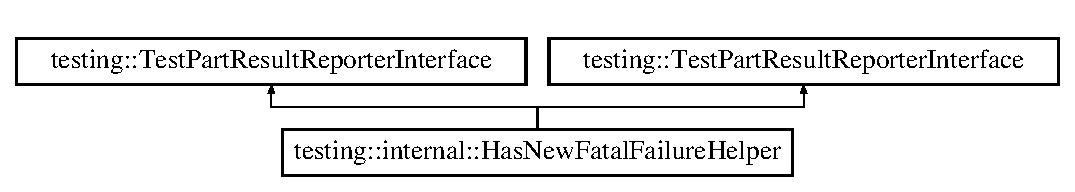
\includegraphics[height=2.000000cm]{classtesting_1_1internal_1_1_has_new_fatal_failure_helper}
\end{center}
\end{figure}
\subsection*{Public Member Functions}
\begin{DoxyCompactItemize}
\item 
\hypertarget{classtesting_1_1internal_1_1_has_new_fatal_failure_helper_ac7b5e77c9847b2b057cb97193ba82441}{}virtual void {\bfseries Report\+Test\+Part\+Result} (const \hyperlink{classtesting_1_1_test_part_result}{Test\+Part\+Result} \&result)\label{classtesting_1_1internal_1_1_has_new_fatal_failure_helper_ac7b5e77c9847b2b057cb97193ba82441}

\item 
\hypertarget{classtesting_1_1internal_1_1_has_new_fatal_failure_helper_ae137e639098071f11f531bbd72dde1c7}{}bool {\bfseries has\+\_\+new\+\_\+fatal\+\_\+failure} () const \label{classtesting_1_1internal_1_1_has_new_fatal_failure_helper_ae137e639098071f11f531bbd72dde1c7}

\item 
\hypertarget{classtesting_1_1internal_1_1_has_new_fatal_failure_helper_ac7b5e77c9847b2b057cb97193ba82441}{}virtual void {\bfseries Report\+Test\+Part\+Result} (const \hyperlink{classtesting_1_1_test_part_result}{Test\+Part\+Result} \&result)\label{classtesting_1_1internal_1_1_has_new_fatal_failure_helper_ac7b5e77c9847b2b057cb97193ba82441}

\item 
\hypertarget{classtesting_1_1internal_1_1_has_new_fatal_failure_helper_ae137e639098071f11f531bbd72dde1c7}{}bool {\bfseries has\+\_\+new\+\_\+fatal\+\_\+failure} () const \label{classtesting_1_1internal_1_1_has_new_fatal_failure_helper_ae137e639098071f11f531bbd72dde1c7}

\end{DoxyCompactItemize}


The documentation for this class was generated from the following file\+:\begin{DoxyCompactItemize}
\item 
deps/win32/debug/include/gtest/gtest-\/test-\/part.\+h\end{DoxyCompactItemize}

\hypertarget{classtesting_1_1internal_1_1_implicitly_convertible}{}\section{testing\+:\+:internal\+:\+:Implicitly\+Convertible$<$ From, To $>$ Class Template Reference}
\label{classtesting_1_1internal_1_1_implicitly_convertible}\index{testing\+::internal\+::\+Implicitly\+Convertible$<$ From, To $>$@{testing\+::internal\+::\+Implicitly\+Convertible$<$ From, To $>$}}
\subsection*{Static Public Attributes}
\begin{DoxyCompactItemize}
\item 
static const bool {\bfseries value}
\end{DoxyCompactItemize}


\subsection{Member Data Documentation}
\hypertarget{classtesting_1_1internal_1_1_implicitly_convertible_aea51cecabca681fb75659e224771b7b7}{}\index{testing\+::internal\+::\+Implicitly\+Convertible@{testing\+::internal\+::\+Implicitly\+Convertible}!value@{value}}
\index{value@{value}!testing\+::internal\+::\+Implicitly\+Convertible@{testing\+::internal\+::\+Implicitly\+Convertible}}
\subsubsection[{value}]{\setlength{\rightskip}{0pt plus 5cm}template$<$typename From , typename To $>$ const bool {\bf testing\+::internal\+::\+Implicitly\+Convertible}$<$ From, To $>$\+::value\hspace{0.3cm}{\ttfamily [static]}}\label{classtesting_1_1internal_1_1_implicitly_convertible_aea51cecabca681fb75659e224771b7b7}
{\bfseries Initial value\+:}
\begin{DoxyCode}
=
      \textcolor{keyword}{sizeof}(Helper(ImplicitlyConvertible::MakeFrom())) == 1
\end{DoxyCode}


The documentation for this class was generated from the following file\+:\begin{DoxyCompactItemize}
\item 
deps/win32/debug/include/gtest/internal/gtest-\/internal.\+h\end{DoxyCompactItemize}

\hypertarget{classmm_1_1_i_point}{}\section{mm\+:\+:I\+Point Class Reference}
\label{classmm_1_1_i_point}\index{mm\+::\+I\+Point@{mm\+::\+I\+Point}}
\subsection*{Public Member Functions}
\begin{DoxyCompactItemize}
\item 
\hypertarget{classmm_1_1_i_point_ac62d2faccc100d72d4b93855d389c3bf}{}{\bfseries I\+Point} (int x, int y)\label{classmm_1_1_i_point_ac62d2faccc100d72d4b93855d389c3bf}

\end{DoxyCompactItemize}
\subsection*{Public Attributes}
\begin{DoxyCompactItemize}
\item 
\hypertarget{classmm_1_1_i_point_a27a375fbf08279125fa729f0337f30cb}{}int {\bfseries x}\label{classmm_1_1_i_point_a27a375fbf08279125fa729f0337f30cb}

\item 
\hypertarget{classmm_1_1_i_point_a9bb6a4bf0eaf73154558dcd379a2e9b1}{}int {\bfseries y}\label{classmm_1_1_i_point_a9bb6a4bf0eaf73154558dcd379a2e9b1}

\end{DoxyCompactItemize}


The documentation for this class was generated from the following file\+:\begin{DoxyCompactItemize}
\item 
src/core/mm\+\_\+utils.\+h\end{DoxyCompactItemize}

\hypertarget{classmm_1_1_i_rect}{}\section{mm\+:\+:I\+Rect Class Reference}
\label{classmm_1_1_i_rect}\index{mm\+::\+I\+Rect@{mm\+::\+I\+Rect}}
\subsection*{Public Member Functions}
\begin{DoxyCompactItemize}
\item 
\hypertarget{classmm_1_1_i_rect_ac75013bbed3fe8e6dec3b8bbc6e23f30}{}{\bfseries I\+Rect} (int x, int y, int w, int h)\label{classmm_1_1_i_rect_ac75013bbed3fe8e6dec3b8bbc6e23f30}

\end{DoxyCompactItemize}
\subsection*{Public Attributes}
\begin{DoxyCompactItemize}
\item 
\hypertarget{classmm_1_1_i_rect_a11dd5b0a710f2e9d38867d4831a6a4d0}{}int {\bfseries x}\label{classmm_1_1_i_rect_a11dd5b0a710f2e9d38867d4831a6a4d0}

\item 
\hypertarget{classmm_1_1_i_rect_a1c8d2b62e7105b1ec63e44cbcb472f2f}{}int {\bfseries y}\label{classmm_1_1_i_rect_a1c8d2b62e7105b1ec63e44cbcb472f2f}

\item 
\hypertarget{classmm_1_1_i_rect_ab151e39613a7f4c830c086ee6f11f38d}{}int {\bfseries w}\label{classmm_1_1_i_rect_ab151e39613a7f4c830c086ee6f11f38d}

\item 
\hypertarget{classmm_1_1_i_rect_a33768c8133beb1d17e14e60a76e49635}{}int {\bfseries h}\label{classmm_1_1_i_rect_a33768c8133beb1d17e14e60a76e49635}

\end{DoxyCompactItemize}


The documentation for this class was generated from the following file\+:\begin{DoxyCompactItemize}
\item 
src/core/mm\+\_\+utils.\+h\end{DoxyCompactItemize}

\hypertarget{structtesting_1_1internal_1_1is__pointer}{}\section{testing\+:\+:internal\+:\+:is\+\_\+pointer$<$ T $>$ Struct Template Reference}
\label{structtesting_1_1internal_1_1is__pointer}\index{testing\+::internal\+::is\+\_\+pointer$<$ T $>$@{testing\+::internal\+::is\+\_\+pointer$<$ T $>$}}
Inheritance diagram for testing\+:\+:internal\+:\+:is\+\_\+pointer$<$ T $>$\+:\begin{figure}[H]
\begin{center}
\leavevmode
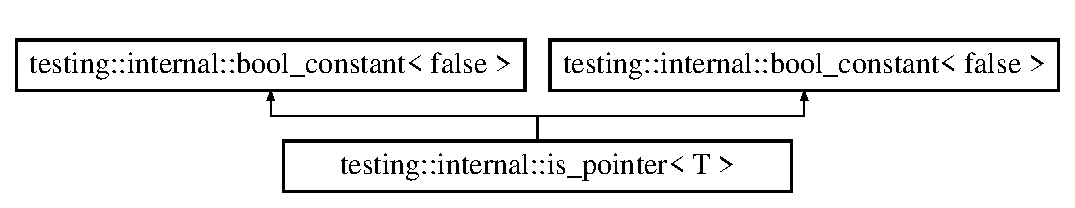
\includegraphics[height=2.000000cm]{structtesting_1_1internal_1_1is__pointer}
\end{center}
\end{figure}
\subsection*{Additional Inherited Members}


The documentation for this struct was generated from the following file\+:\begin{DoxyCompactItemize}
\item 
deps/win32/debug/include/gtest/internal/gtest-\/port.\+h\end{DoxyCompactItemize}

\hypertarget{structtesting_1_1internal_1_1is__pointer_3_01_t_01_5_01_4}{}\section{testing\+:\+:internal\+:\+:is\+\_\+pointer$<$ T $\ast$ $>$ Struct Template Reference}
\label{structtesting_1_1internal_1_1is__pointer_3_01_t_01_5_01_4}\index{testing\+::internal\+::is\+\_\+pointer$<$ T $\ast$ $>$@{testing\+::internal\+::is\+\_\+pointer$<$ T $\ast$ $>$}}
Inheritance diagram for testing\+:\+:internal\+:\+:is\+\_\+pointer$<$ T $\ast$ $>$\+:\begin{figure}[H]
\begin{center}
\leavevmode
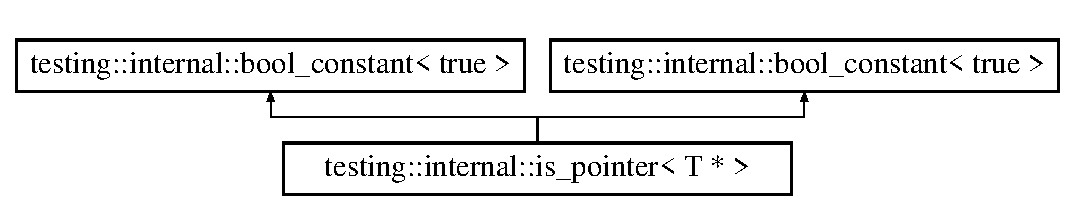
\includegraphics[height=2.000000cm]{structtesting_1_1internal_1_1is__pointer_3_01_t_01_5_01_4}
\end{center}
\end{figure}
\subsection*{Additional Inherited Members}


The documentation for this struct was generated from the following file\+:\begin{DoxyCompactItemize}
\item 
deps/win32/debug/include/gtest/internal/gtest-\/port.\+h\end{DoxyCompactItemize}

\hypertarget{structtesting_1_1internal_1_1_is_a_protocol_message}{}\section{testing\+:\+:internal\+:\+:Is\+A\+Protocol\+Message$<$ T $>$ Struct Template Reference}
\label{structtesting_1_1internal_1_1_is_a_protocol_message}\index{testing\+::internal\+::\+Is\+A\+Protocol\+Message$<$ T $>$@{testing\+::internal\+::\+Is\+A\+Protocol\+Message$<$ T $>$}}
Inheritance diagram for testing\+:\+:internal\+:\+:Is\+A\+Protocol\+Message$<$ T $>$\+:\begin{figure}[H]
\begin{center}
\leavevmode
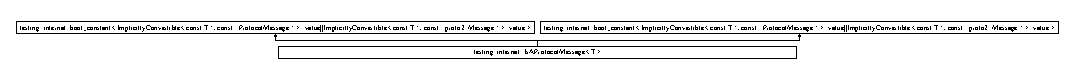
\includegraphics[height=0.566229cm]{structtesting_1_1internal_1_1_is_a_protocol_message}
\end{center}
\end{figure}
\subsection*{Additional Inherited Members}


The documentation for this struct was generated from the following file\+:\begin{DoxyCompactItemize}
\item 
deps/win32/debug/include/gtest/internal/gtest-\/internal.\+h\end{DoxyCompactItemize}

\hypertarget{structtesting_1_1internal_1_1_iterator_traits}{}\section{testing\+:\+:internal\+:\+:Iterator\+Traits$<$ Iterator $>$ Struct Template Reference}
\label{structtesting_1_1internal_1_1_iterator_traits}\index{testing\+::internal\+::\+Iterator\+Traits$<$ Iterator $>$@{testing\+::internal\+::\+Iterator\+Traits$<$ Iterator $>$}}
\subsection*{Public Types}
\begin{DoxyCompactItemize}
\item 
\hypertarget{structtesting_1_1internal_1_1_iterator_traits_a29de4320a9c53ce438d3561b94e515bb}{}typedef Iterator\+::value\+\_\+type {\bfseries value\+\_\+type}\label{structtesting_1_1internal_1_1_iterator_traits_a29de4320a9c53ce438d3561b94e515bb}

\item 
\hypertarget{structtesting_1_1internal_1_1_iterator_traits_a29de4320a9c53ce438d3561b94e515bb}{}typedef Iterator\+::value\+\_\+type {\bfseries value\+\_\+type}\label{structtesting_1_1internal_1_1_iterator_traits_a29de4320a9c53ce438d3561b94e515bb}

\end{DoxyCompactItemize}


The documentation for this struct was generated from the following file\+:\begin{DoxyCompactItemize}
\item 
deps/win32/debug/include/gtest/internal/gtest-\/port.\+h\end{DoxyCompactItemize}

\hypertarget{structtesting_1_1internal_1_1_iterator_traits_3_01const_01_t_01_5_01_4}{}\section{testing\+:\+:internal\+:\+:Iterator\+Traits$<$ const T $\ast$ $>$ Struct Template Reference}
\label{structtesting_1_1internal_1_1_iterator_traits_3_01const_01_t_01_5_01_4}\index{testing\+::internal\+::\+Iterator\+Traits$<$ const T $\ast$ $>$@{testing\+::internal\+::\+Iterator\+Traits$<$ const T $\ast$ $>$}}
\subsection*{Public Types}
\begin{DoxyCompactItemize}
\item 
\hypertarget{structtesting_1_1internal_1_1_iterator_traits_3_01const_01_t_01_5_01_4_ae7c8867223e106f374b56a7dc4a85547}{}typedef T {\bfseries value\+\_\+type}\label{structtesting_1_1internal_1_1_iterator_traits_3_01const_01_t_01_5_01_4_ae7c8867223e106f374b56a7dc4a85547}

\item 
\hypertarget{structtesting_1_1internal_1_1_iterator_traits_3_01const_01_t_01_5_01_4_ae7c8867223e106f374b56a7dc4a85547}{}typedef T {\bfseries value\+\_\+type}\label{structtesting_1_1internal_1_1_iterator_traits_3_01const_01_t_01_5_01_4_ae7c8867223e106f374b56a7dc4a85547}

\end{DoxyCompactItemize}


The documentation for this struct was generated from the following file\+:\begin{DoxyCompactItemize}
\item 
deps/win32/debug/include/gtest/internal/gtest-\/port.\+h\end{DoxyCompactItemize}

\hypertarget{structtesting_1_1internal_1_1_iterator_traits_3_01_t_01_5_01_4}{}\section{testing\+:\+:internal\+:\+:Iterator\+Traits$<$ T $\ast$ $>$ Struct Template Reference}
\label{structtesting_1_1internal_1_1_iterator_traits_3_01_t_01_5_01_4}\index{testing\+::internal\+::\+Iterator\+Traits$<$ T $\ast$ $>$@{testing\+::internal\+::\+Iterator\+Traits$<$ T $\ast$ $>$}}
\subsection*{Public Types}
\begin{DoxyCompactItemize}
\item 
\hypertarget{structtesting_1_1internal_1_1_iterator_traits_3_01_t_01_5_01_4_a7e46869ed36cc5aea898e243d270a8be}{}typedef T {\bfseries value\+\_\+type}\label{structtesting_1_1internal_1_1_iterator_traits_3_01_t_01_5_01_4_a7e46869ed36cc5aea898e243d270a8be}

\item 
\hypertarget{structtesting_1_1internal_1_1_iterator_traits_3_01_t_01_5_01_4_a7e46869ed36cc5aea898e243d270a8be}{}typedef T {\bfseries value\+\_\+type}\label{structtesting_1_1internal_1_1_iterator_traits_3_01_t_01_5_01_4_a7e46869ed36cc5aea898e243d270a8be}

\end{DoxyCompactItemize}


The documentation for this struct was generated from the following file\+:\begin{DoxyCompactItemize}
\item 
deps/win32/debug/include/gtest/internal/gtest-\/port.\+h\end{DoxyCompactItemize}

\hypertarget{classtesting_1_1internal_1_1linked__ptr}{}\section{testing\+:\+:internal\+:\+:linked\+\_\+ptr$<$ T $>$ Class Template Reference}
\label{classtesting_1_1internal_1_1linked__ptr}\index{testing\+::internal\+::linked\+\_\+ptr$<$ T $>$@{testing\+::internal\+::linked\+\_\+ptr$<$ T $>$}}
\subsection*{Public Types}
\begin{DoxyCompactItemize}
\item 
\hypertarget{classtesting_1_1internal_1_1linked__ptr_a295c7d1ee4100d916514c4e4385a0063}{}typedef T {\bfseries element\+\_\+type}\label{classtesting_1_1internal_1_1linked__ptr_a295c7d1ee4100d916514c4e4385a0063}

\item 
\hypertarget{classtesting_1_1internal_1_1linked__ptr_a295c7d1ee4100d916514c4e4385a0063}{}typedef T {\bfseries element\+\_\+type}\label{classtesting_1_1internal_1_1linked__ptr_a295c7d1ee4100d916514c4e4385a0063}

\end{DoxyCompactItemize}
\subsection*{Public Member Functions}
\begin{DoxyCompactItemize}
\item 
\hypertarget{classtesting_1_1internal_1_1linked__ptr_ae805418b9f03f14ff49649e710475dba}{}{\bfseries linked\+\_\+ptr} (T $\ast$ptr=N\+U\+L\+L)\label{classtesting_1_1internal_1_1linked__ptr_ae805418b9f03f14ff49649e710475dba}

\item 
\hypertarget{classtesting_1_1internal_1_1linked__ptr_a7597ed91006edd0467c99bd1aaab07f5}{}{\footnotesize template$<$typename U $>$ }\\{\bfseries linked\+\_\+ptr} (\hyperlink{classtesting_1_1internal_1_1linked__ptr}{linked\+\_\+ptr}$<$ U $>$ const \&ptr)\label{classtesting_1_1internal_1_1linked__ptr_a7597ed91006edd0467c99bd1aaab07f5}

\item 
\hypertarget{classtesting_1_1internal_1_1linked__ptr_abc076b5678cc7f64306d5ecfefc93aff}{}{\bfseries linked\+\_\+ptr} (\hyperlink{classtesting_1_1internal_1_1linked__ptr}{linked\+\_\+ptr} const \&ptr)\label{classtesting_1_1internal_1_1linked__ptr_abc076b5678cc7f64306d5ecfefc93aff}

\item 
\hypertarget{classtesting_1_1internal_1_1linked__ptr_a82608d98869b750d9ab729f1450a9a45}{}{\footnotesize template$<$typename U $>$ }\\\hyperlink{classtesting_1_1internal_1_1linked__ptr}{linked\+\_\+ptr} \& {\bfseries operator=} (\hyperlink{classtesting_1_1internal_1_1linked__ptr}{linked\+\_\+ptr}$<$ U $>$ const \&ptr)\label{classtesting_1_1internal_1_1linked__ptr_a82608d98869b750d9ab729f1450a9a45}

\item 
\hypertarget{classtesting_1_1internal_1_1linked__ptr_a1f40b5e66e6cf7b661ea116c806f952e}{}\hyperlink{classtesting_1_1internal_1_1linked__ptr}{linked\+\_\+ptr} \& {\bfseries operator=} (\hyperlink{classtesting_1_1internal_1_1linked__ptr}{linked\+\_\+ptr} const \&ptr)\label{classtesting_1_1internal_1_1linked__ptr_a1f40b5e66e6cf7b661ea116c806f952e}

\item 
\hypertarget{classtesting_1_1internal_1_1linked__ptr_a95ba3b7b66ed0193c779976c6e126ab6}{}void {\bfseries reset} (T $\ast$ptr=N\+U\+L\+L)\label{classtesting_1_1internal_1_1linked__ptr_a95ba3b7b66ed0193c779976c6e126ab6}

\item 
\hypertarget{classtesting_1_1internal_1_1linked__ptr_a6ea8584d9bcad13c3266834f5ce5e771}{}T $\ast$ {\bfseries get} () const \label{classtesting_1_1internal_1_1linked__ptr_a6ea8584d9bcad13c3266834f5ce5e771}

\item 
\hypertarget{classtesting_1_1internal_1_1linked__ptr_aa878c3e874242fb3cd2aa14ec603aa25}{}T $\ast$ {\bfseries operator-\/$>$} () const \label{classtesting_1_1internal_1_1linked__ptr_aa878c3e874242fb3cd2aa14ec603aa25}

\item 
\hypertarget{classtesting_1_1internal_1_1linked__ptr_aec393cbd60f96defde36ef8a69d94254}{}T \& {\bfseries operator$\ast$} () const \label{classtesting_1_1internal_1_1linked__ptr_aec393cbd60f96defde36ef8a69d94254}

\item 
\hypertarget{classtesting_1_1internal_1_1linked__ptr_abe2154fd3ad3574dfe6f2320bc1debc4}{}bool {\bfseries operator==} (T $\ast$p) const \label{classtesting_1_1internal_1_1linked__ptr_abe2154fd3ad3574dfe6f2320bc1debc4}

\item 
\hypertarget{classtesting_1_1internal_1_1linked__ptr_a3685f9661bbe410cfa58fea2f14396b7}{}bool {\bfseries operator!=} (T $\ast$p) const \label{classtesting_1_1internal_1_1linked__ptr_a3685f9661bbe410cfa58fea2f14396b7}

\item 
\hypertarget{classtesting_1_1internal_1_1linked__ptr_a3b46c9ecfd928673a524dcb3c70fd2ad}{}{\footnotesize template$<$typename U $>$ }\\bool {\bfseries operator==} (\hyperlink{classtesting_1_1internal_1_1linked__ptr}{linked\+\_\+ptr}$<$ U $>$ const \&ptr) const \label{classtesting_1_1internal_1_1linked__ptr_a3b46c9ecfd928673a524dcb3c70fd2ad}

\item 
\hypertarget{classtesting_1_1internal_1_1linked__ptr_a6449584b90a09a313300599fb3a23633}{}{\footnotesize template$<$typename U $>$ }\\bool {\bfseries operator!=} (\hyperlink{classtesting_1_1internal_1_1linked__ptr}{linked\+\_\+ptr}$<$ U $>$ const \&ptr) const \label{classtesting_1_1internal_1_1linked__ptr_a6449584b90a09a313300599fb3a23633}

\item 
\hypertarget{classtesting_1_1internal_1_1linked__ptr_ae805418b9f03f14ff49649e710475dba}{}{\bfseries linked\+\_\+ptr} (T $\ast$ptr=N\+U\+L\+L)\label{classtesting_1_1internal_1_1linked__ptr_ae805418b9f03f14ff49649e710475dba}

\item 
\hypertarget{classtesting_1_1internal_1_1linked__ptr_a7597ed91006edd0467c99bd1aaab07f5}{}{\footnotesize template$<$typename U $>$ }\\{\bfseries linked\+\_\+ptr} (\hyperlink{classtesting_1_1internal_1_1linked__ptr}{linked\+\_\+ptr}$<$ U $>$ const \&ptr)\label{classtesting_1_1internal_1_1linked__ptr_a7597ed91006edd0467c99bd1aaab07f5}

\item 
\hypertarget{classtesting_1_1internal_1_1linked__ptr_abc076b5678cc7f64306d5ecfefc93aff}{}{\bfseries linked\+\_\+ptr} (\hyperlink{classtesting_1_1internal_1_1linked__ptr}{linked\+\_\+ptr} const \&ptr)\label{classtesting_1_1internal_1_1linked__ptr_abc076b5678cc7f64306d5ecfefc93aff}

\item 
\hypertarget{classtesting_1_1internal_1_1linked__ptr_a82608d98869b750d9ab729f1450a9a45}{}{\footnotesize template$<$typename U $>$ }\\\hyperlink{classtesting_1_1internal_1_1linked__ptr}{linked\+\_\+ptr} \& {\bfseries operator=} (\hyperlink{classtesting_1_1internal_1_1linked__ptr}{linked\+\_\+ptr}$<$ U $>$ const \&ptr)\label{classtesting_1_1internal_1_1linked__ptr_a82608d98869b750d9ab729f1450a9a45}

\item 
\hypertarget{classtesting_1_1internal_1_1linked__ptr_a1f40b5e66e6cf7b661ea116c806f952e}{}\hyperlink{classtesting_1_1internal_1_1linked__ptr}{linked\+\_\+ptr} \& {\bfseries operator=} (\hyperlink{classtesting_1_1internal_1_1linked__ptr}{linked\+\_\+ptr} const \&ptr)\label{classtesting_1_1internal_1_1linked__ptr_a1f40b5e66e6cf7b661ea116c806f952e}

\item 
\hypertarget{classtesting_1_1internal_1_1linked__ptr_a95ba3b7b66ed0193c779976c6e126ab6}{}void {\bfseries reset} (T $\ast$ptr=N\+U\+L\+L)\label{classtesting_1_1internal_1_1linked__ptr_a95ba3b7b66ed0193c779976c6e126ab6}

\item 
\hypertarget{classtesting_1_1internal_1_1linked__ptr_a6ea8584d9bcad13c3266834f5ce5e771}{}T $\ast$ {\bfseries get} () const \label{classtesting_1_1internal_1_1linked__ptr_a6ea8584d9bcad13c3266834f5ce5e771}

\item 
\hypertarget{classtesting_1_1internal_1_1linked__ptr_aa878c3e874242fb3cd2aa14ec603aa25}{}T $\ast$ {\bfseries operator-\/$>$} () const \label{classtesting_1_1internal_1_1linked__ptr_aa878c3e874242fb3cd2aa14ec603aa25}

\item 
\hypertarget{classtesting_1_1internal_1_1linked__ptr_aec393cbd60f96defde36ef8a69d94254}{}T \& {\bfseries operator$\ast$} () const \label{classtesting_1_1internal_1_1linked__ptr_aec393cbd60f96defde36ef8a69d94254}

\item 
\hypertarget{classtesting_1_1internal_1_1linked__ptr_abe2154fd3ad3574dfe6f2320bc1debc4}{}bool {\bfseries operator==} (T $\ast$p) const \label{classtesting_1_1internal_1_1linked__ptr_abe2154fd3ad3574dfe6f2320bc1debc4}

\item 
\hypertarget{classtesting_1_1internal_1_1linked__ptr_a3685f9661bbe410cfa58fea2f14396b7}{}bool {\bfseries operator!=} (T $\ast$p) const \label{classtesting_1_1internal_1_1linked__ptr_a3685f9661bbe410cfa58fea2f14396b7}

\item 
\hypertarget{classtesting_1_1internal_1_1linked__ptr_a3b46c9ecfd928673a524dcb3c70fd2ad}{}{\footnotesize template$<$typename U $>$ }\\bool {\bfseries operator==} (\hyperlink{classtesting_1_1internal_1_1linked__ptr}{linked\+\_\+ptr}$<$ U $>$ const \&ptr) const \label{classtesting_1_1internal_1_1linked__ptr_a3b46c9ecfd928673a524dcb3c70fd2ad}

\item 
\hypertarget{classtesting_1_1internal_1_1linked__ptr_a6449584b90a09a313300599fb3a23633}{}{\footnotesize template$<$typename U $>$ }\\bool {\bfseries operator!=} (\hyperlink{classtesting_1_1internal_1_1linked__ptr}{linked\+\_\+ptr}$<$ U $>$ const \&ptr) const \label{classtesting_1_1internal_1_1linked__ptr_a6449584b90a09a313300599fb3a23633}

\end{DoxyCompactItemize}
\subsection*{Friends}
\begin{DoxyCompactItemize}
\item 
\hypertarget{classtesting_1_1internal_1_1linked__ptr_a7763f286ca03a7f7363a033d996c8c1c}{}{\footnotesize template$<$typename U $>$ }\\class {\bfseries linked\+\_\+ptr}\label{classtesting_1_1internal_1_1linked__ptr_a7763f286ca03a7f7363a033d996c8c1c}

\end{DoxyCompactItemize}


The documentation for this class was generated from the following file\+:\begin{DoxyCompactItemize}
\item 
deps/win32/debug/include/gtest/internal/gtest-\/linked\+\_\+ptr.\+h\end{DoxyCompactItemize}

\hypertarget{classtesting_1_1internal_1_1linked__ptr__internal}{}\section{testing\+:\+:internal\+:\+:linked\+\_\+ptr\+\_\+internal Class Reference}
\label{classtesting_1_1internal_1_1linked__ptr__internal}\index{testing\+::internal\+::linked\+\_\+ptr\+\_\+internal@{testing\+::internal\+::linked\+\_\+ptr\+\_\+internal}}
\subsection*{Public Member Functions}
\begin{DoxyCompactItemize}
\item 
\hypertarget{classtesting_1_1internal_1_1linked__ptr__internal_a742af1f65df2d5e2b7198a1b74264a83}{}void {\bfseries join\+\_\+new} ()\label{classtesting_1_1internal_1_1linked__ptr__internal_a742af1f65df2d5e2b7198a1b74264a83}

\item 
\hypertarget{classtesting_1_1internal_1_1linked__ptr__internal_acd5a341459f7e81b10b4112d8c764e2a}{}void {\bfseries join} (\hyperlink{classtesting_1_1internal_1_1linked__ptr__internal}{linked\+\_\+ptr\+\_\+internal} const $\ast$ptr) G\+T\+E\+S\+T\+\_\+\+L\+O\+C\+K\+\_\+\+E\+X\+C\+L\+U\+D\+E\+D\+\_\+(g\+\_\+linked\+\_\+ptr\+\_\+mutex)\label{classtesting_1_1internal_1_1linked__ptr__internal_acd5a341459f7e81b10b4112d8c764e2a}

\item 
\hypertarget{classtesting_1_1internal_1_1linked__ptr__internal_a8699e539d9702d363ef0351012d1b3ca}{}bool {\bfseries depart} () G\+T\+E\+S\+T\+\_\+\+L\+O\+C\+K\+\_\+\+E\+X\+C\+L\+U\+D\+E\+D\+\_\+(g\+\_\+linked\+\_\+ptr\+\_\+mutex)\label{classtesting_1_1internal_1_1linked__ptr__internal_a8699e539d9702d363ef0351012d1b3ca}

\item 
\hypertarget{classtesting_1_1internal_1_1linked__ptr__internal_a742af1f65df2d5e2b7198a1b74264a83}{}void {\bfseries join\+\_\+new} ()\label{classtesting_1_1internal_1_1linked__ptr__internal_a742af1f65df2d5e2b7198a1b74264a83}

\item 
\hypertarget{classtesting_1_1internal_1_1linked__ptr__internal_acd5a341459f7e81b10b4112d8c764e2a}{}void {\bfseries join} (\hyperlink{classtesting_1_1internal_1_1linked__ptr__internal}{linked\+\_\+ptr\+\_\+internal} const $\ast$ptr) G\+T\+E\+S\+T\+\_\+\+L\+O\+C\+K\+\_\+\+E\+X\+C\+L\+U\+D\+E\+D\+\_\+(g\+\_\+linked\+\_\+ptr\+\_\+mutex)\label{classtesting_1_1internal_1_1linked__ptr__internal_acd5a341459f7e81b10b4112d8c764e2a}

\item 
\hypertarget{classtesting_1_1internal_1_1linked__ptr__internal_a8699e539d9702d363ef0351012d1b3ca}{}bool {\bfseries depart} () G\+T\+E\+S\+T\+\_\+\+L\+O\+C\+K\+\_\+\+E\+X\+C\+L\+U\+D\+E\+D\+\_\+(g\+\_\+linked\+\_\+ptr\+\_\+mutex)\label{classtesting_1_1internal_1_1linked__ptr__internal_a8699e539d9702d363ef0351012d1b3ca}

\end{DoxyCompactItemize}


The documentation for this class was generated from the following file\+:\begin{DoxyCompactItemize}
\item 
deps/win32/debug/include/gtest/internal/gtest-\/linked\+\_\+ptr.\+h\end{DoxyCompactItemize}

\hypertarget{classtesting_1_1_message}{}\section{testing\+:\+:Message Class Reference}
\label{classtesting_1_1_message}\index{testing\+::\+Message@{testing\+::\+Message}}
\subsection*{Public Member Functions}
\begin{DoxyCompactItemize}
\item 
\hypertarget{classtesting_1_1_message_ac126e24804817a053bebba0920d94a11}{}{\bfseries Message} (const \hyperlink{classtesting_1_1_message}{Message} \&msg)\label{classtesting_1_1_message_ac126e24804817a053bebba0920d94a11}

\item 
\hypertarget{classtesting_1_1_message_a9de694ca239486809fc99fbbea8ac21d}{}{\bfseries Message} (const char $\ast$str)\label{classtesting_1_1_message_a9de694ca239486809fc99fbbea8ac21d}

\item 
\hypertarget{classtesting_1_1_message_a2e0e71be52d54c20a75a55fca812721f}{}{\footnotesize template$<$typename T $>$ }\\\hyperlink{classtesting_1_1_message}{Message} \& {\bfseries operator$<$$<$} (const T \&val)\label{classtesting_1_1_message_a2e0e71be52d54c20a75a55fca812721f}

\item 
\hypertarget{classtesting_1_1_message_aa3ab685879958f90d2d8cd5b68d10c34}{}{\footnotesize template$<$typename T $>$ }\\\hyperlink{classtesting_1_1_message}{Message} \& {\bfseries operator$<$$<$} (T $\ast$const \&pointer)\label{classtesting_1_1_message_aa3ab685879958f90d2d8cd5b68d10c34}

\item 
\hypertarget{classtesting_1_1_message_a3a71a1c1c8ea52de5852d75483d41453}{}\hyperlink{classtesting_1_1_message}{Message} \& {\bfseries operator$<$$<$} (Basic\+Narrow\+Io\+Manip val)\label{classtesting_1_1_message_a3a71a1c1c8ea52de5852d75483d41453}

\item 
\hypertarget{classtesting_1_1_message_a3e1e04f23b1bdfe18adfd59928296346}{}\hyperlink{classtesting_1_1_message}{Message} \& {\bfseries operator$<$$<$} (bool b)\label{classtesting_1_1_message_a3e1e04f23b1bdfe18adfd59928296346}

\item 
\hypertarget{classtesting_1_1_message_a34774e225944cb6df02db9689d312aae}{}\hyperlink{classtesting_1_1_message}{Message} \& {\bfseries operator$<$$<$} (const wchar\+\_\+t $\ast$wide\+\_\+c\+\_\+str)\label{classtesting_1_1_message_a34774e225944cb6df02db9689d312aae}

\item 
\hypertarget{classtesting_1_1_message_aae57eefb3a72a19c11453d630b1d846c}{}\hyperlink{classtesting_1_1_message}{Message} \& {\bfseries operator$<$$<$} (wchar\+\_\+t $\ast$wide\+\_\+c\+\_\+str)\label{classtesting_1_1_message_aae57eefb3a72a19c11453d630b1d846c}

\item 
\hypertarget{classtesting_1_1_message_abe8c1b7584aa670dd0e2413e8317a937}{}std\+::string {\bfseries Get\+String} () const \label{classtesting_1_1_message_abe8c1b7584aa670dd0e2413e8317a937}

\item 
\hypertarget{classtesting_1_1_message_ac126e24804817a053bebba0920d94a11}{}{\bfseries Message} (const \hyperlink{classtesting_1_1_message}{Message} \&msg)\label{classtesting_1_1_message_ac126e24804817a053bebba0920d94a11}

\item 
\hypertarget{classtesting_1_1_message_a9de694ca239486809fc99fbbea8ac21d}{}{\bfseries Message} (const char $\ast$str)\label{classtesting_1_1_message_a9de694ca239486809fc99fbbea8ac21d}

\item 
\hypertarget{classtesting_1_1_message_a2e0e71be52d54c20a75a55fca812721f}{}{\footnotesize template$<$typename T $>$ }\\\hyperlink{classtesting_1_1_message}{Message} \& {\bfseries operator$<$$<$} (const T \&val)\label{classtesting_1_1_message_a2e0e71be52d54c20a75a55fca812721f}

\item 
\hypertarget{classtesting_1_1_message_aa3ab685879958f90d2d8cd5b68d10c34}{}{\footnotesize template$<$typename T $>$ }\\\hyperlink{classtesting_1_1_message}{Message} \& {\bfseries operator$<$$<$} (T $\ast$const \&pointer)\label{classtesting_1_1_message_aa3ab685879958f90d2d8cd5b68d10c34}

\item 
\hypertarget{classtesting_1_1_message_a3a71a1c1c8ea52de5852d75483d41453}{}\hyperlink{classtesting_1_1_message}{Message} \& {\bfseries operator$<$$<$} (Basic\+Narrow\+Io\+Manip val)\label{classtesting_1_1_message_a3a71a1c1c8ea52de5852d75483d41453}

\item 
\hypertarget{classtesting_1_1_message_a3e1e04f23b1bdfe18adfd59928296346}{}\hyperlink{classtesting_1_1_message}{Message} \& {\bfseries operator$<$$<$} (bool b)\label{classtesting_1_1_message_a3e1e04f23b1bdfe18adfd59928296346}

\item 
\hypertarget{classtesting_1_1_message_a34774e225944cb6df02db9689d312aae}{}\hyperlink{classtesting_1_1_message}{Message} \& {\bfseries operator$<$$<$} (const wchar\+\_\+t $\ast$wide\+\_\+c\+\_\+str)\label{classtesting_1_1_message_a34774e225944cb6df02db9689d312aae}

\item 
\hypertarget{classtesting_1_1_message_aae57eefb3a72a19c11453d630b1d846c}{}\hyperlink{classtesting_1_1_message}{Message} \& {\bfseries operator$<$$<$} (wchar\+\_\+t $\ast$wide\+\_\+c\+\_\+str)\label{classtesting_1_1_message_aae57eefb3a72a19c11453d630b1d846c}

\item 
\hypertarget{classtesting_1_1_message_abe8c1b7584aa670dd0e2413e8317a937}{}std\+::string {\bfseries Get\+String} () const \label{classtesting_1_1_message_abe8c1b7584aa670dd0e2413e8317a937}

\end{DoxyCompactItemize}


The documentation for this class was generated from the following file\+:\begin{DoxyCompactItemize}
\item 
deps/win32/debug/include/gtest/gtest-\/message.\+h\end{DoxyCompactItemize}

\hypertarget{classtesting_1_1internal_1_1_mutex}{}\section{testing\+:\+:internal\+:\+:Mutex Class Reference}
\label{classtesting_1_1internal_1_1_mutex}\index{testing\+::internal\+::\+Mutex@{testing\+::internal\+::\+Mutex}}
\subsection*{Public Member Functions}
\begin{DoxyCompactItemize}
\item 
\hypertarget{classtesting_1_1internal_1_1_mutex_ae7e2191886c00182176b23c4f4d049f8}{}void {\bfseries Lock} ()\label{classtesting_1_1internal_1_1_mutex_ae7e2191886c00182176b23c4f4d049f8}

\item 
\hypertarget{classtesting_1_1internal_1_1_mutex_a315188055de1be98884519ad84eff2e6}{}void {\bfseries Unlock} ()\label{classtesting_1_1internal_1_1_mutex_a315188055de1be98884519ad84eff2e6}

\item 
\hypertarget{classtesting_1_1internal_1_1_mutex_a3a0530bca3110025d85b2aa51f3ca0d7}{}void {\bfseries Assert\+Held} () const \label{classtesting_1_1internal_1_1_mutex_a3a0530bca3110025d85b2aa51f3ca0d7}

\item 
\hypertarget{classtesting_1_1internal_1_1_mutex_ae7e2191886c00182176b23c4f4d049f8}{}void {\bfseries Lock} ()\label{classtesting_1_1internal_1_1_mutex_ae7e2191886c00182176b23c4f4d049f8}

\item 
\hypertarget{classtesting_1_1internal_1_1_mutex_a315188055de1be98884519ad84eff2e6}{}void {\bfseries Unlock} ()\label{classtesting_1_1internal_1_1_mutex_a315188055de1be98884519ad84eff2e6}

\item 
\hypertarget{classtesting_1_1internal_1_1_mutex_a3a0530bca3110025d85b2aa51f3ca0d7}{}void {\bfseries Assert\+Held} () const \label{classtesting_1_1internal_1_1_mutex_a3a0530bca3110025d85b2aa51f3ca0d7}

\end{DoxyCompactItemize}


The documentation for this class was generated from the following file\+:\begin{DoxyCompactItemize}
\item 
deps/win32/debug/include/gtest/internal/gtest-\/port.\+h\end{DoxyCompactItemize}

\hypertarget{classtesting_1_1internal_1_1_native_array}{}\section{testing\+:\+:internal\+:\+:Native\+Array$<$ Element $>$ Class Template Reference}
\label{classtesting_1_1internal_1_1_native_array}\index{testing\+::internal\+::\+Native\+Array$<$ Element $>$@{testing\+::internal\+::\+Native\+Array$<$ Element $>$}}
\subsection*{Public Types}
\begin{DoxyCompactItemize}
\item 
\hypertarget{classtesting_1_1internal_1_1_native_array_a12216d686e16e4cc63d952fada5b2ba9}{}typedef Element {\bfseries value\+\_\+type}\label{classtesting_1_1internal_1_1_native_array_a12216d686e16e4cc63d952fada5b2ba9}

\item 
\hypertarget{classtesting_1_1internal_1_1_native_array_ac1301a57977b57a1ad013e4e25fc2a72}{}typedef Element $\ast$ {\bfseries iterator}\label{classtesting_1_1internal_1_1_native_array_ac1301a57977b57a1ad013e4e25fc2a72}

\item 
\hypertarget{classtesting_1_1internal_1_1_native_array_a9ce7c8408460d7158a2870456d134557}{}typedef const Element $\ast$ {\bfseries const\+\_\+iterator}\label{classtesting_1_1internal_1_1_native_array_a9ce7c8408460d7158a2870456d134557}

\item 
\hypertarget{classtesting_1_1internal_1_1_native_array_a12216d686e16e4cc63d952fada5b2ba9}{}typedef Element {\bfseries value\+\_\+type}\label{classtesting_1_1internal_1_1_native_array_a12216d686e16e4cc63d952fada5b2ba9}

\item 
\hypertarget{classtesting_1_1internal_1_1_native_array_ac1301a57977b57a1ad013e4e25fc2a72}{}typedef Element $\ast$ {\bfseries iterator}\label{classtesting_1_1internal_1_1_native_array_ac1301a57977b57a1ad013e4e25fc2a72}

\item 
\hypertarget{classtesting_1_1internal_1_1_native_array_a9ce7c8408460d7158a2870456d134557}{}typedef const Element $\ast$ {\bfseries const\+\_\+iterator}\label{classtesting_1_1internal_1_1_native_array_a9ce7c8408460d7158a2870456d134557}

\end{DoxyCompactItemize}
\subsection*{Public Member Functions}
\begin{DoxyCompactItemize}
\item 
\hypertarget{classtesting_1_1internal_1_1_native_array_a568de999aca0fc0c2cc574fac2405872}{}{\bfseries Native\+Array} (const Element $\ast$array, size\+\_\+t count, Relation\+To\+Source relation)\label{classtesting_1_1internal_1_1_native_array_a568de999aca0fc0c2cc574fac2405872}

\item 
\hypertarget{classtesting_1_1internal_1_1_native_array_abb346ac3040f5da733f594cc2d5958bc}{}{\bfseries Native\+Array} (const \hyperlink{classtesting_1_1internal_1_1_native_array}{Native\+Array} \&rhs)\label{classtesting_1_1internal_1_1_native_array_abb346ac3040f5da733f594cc2d5958bc}

\item 
\hypertarget{classtesting_1_1internal_1_1_native_array_a45de2485baac8bf148e2943828094a40}{}size\+\_\+t {\bfseries size} () const \label{classtesting_1_1internal_1_1_native_array_a45de2485baac8bf148e2943828094a40}

\item 
\hypertarget{classtesting_1_1internal_1_1_native_array_a49c534d29034d9230372ada54ef961bb}{}const\+\_\+iterator {\bfseries begin} () const \label{classtesting_1_1internal_1_1_native_array_a49c534d29034d9230372ada54ef961bb}

\item 
\hypertarget{classtesting_1_1internal_1_1_native_array_a4957ad1ebf7c21eab07d5e0ae2bb17aa}{}const\+\_\+iterator {\bfseries end} () const \label{classtesting_1_1internal_1_1_native_array_a4957ad1ebf7c21eab07d5e0ae2bb17aa}

\item 
\hypertarget{classtesting_1_1internal_1_1_native_array_a60af8d9c429771ee131b5ddf7e06e3c9}{}bool {\bfseries operator==} (const \hyperlink{classtesting_1_1internal_1_1_native_array}{Native\+Array} \&rhs) const \label{classtesting_1_1internal_1_1_native_array_a60af8d9c429771ee131b5ddf7e06e3c9}

\item 
\hypertarget{classtesting_1_1internal_1_1_native_array_a568de999aca0fc0c2cc574fac2405872}{}{\bfseries Native\+Array} (const Element $\ast$array, size\+\_\+t count, Relation\+To\+Source relation)\label{classtesting_1_1internal_1_1_native_array_a568de999aca0fc0c2cc574fac2405872}

\item 
\hypertarget{classtesting_1_1internal_1_1_native_array_abb346ac3040f5da733f594cc2d5958bc}{}{\bfseries Native\+Array} (const \hyperlink{classtesting_1_1internal_1_1_native_array}{Native\+Array} \&rhs)\label{classtesting_1_1internal_1_1_native_array_abb346ac3040f5da733f594cc2d5958bc}

\item 
\hypertarget{classtesting_1_1internal_1_1_native_array_a45de2485baac8bf148e2943828094a40}{}size\+\_\+t {\bfseries size} () const \label{classtesting_1_1internal_1_1_native_array_a45de2485baac8bf148e2943828094a40}

\item 
\hypertarget{classtesting_1_1internal_1_1_native_array_a49c534d29034d9230372ada54ef961bb}{}const\+\_\+iterator {\bfseries begin} () const \label{classtesting_1_1internal_1_1_native_array_a49c534d29034d9230372ada54ef961bb}

\item 
\hypertarget{classtesting_1_1internal_1_1_native_array_a4957ad1ebf7c21eab07d5e0ae2bb17aa}{}const\+\_\+iterator {\bfseries end} () const \label{classtesting_1_1internal_1_1_native_array_a4957ad1ebf7c21eab07d5e0ae2bb17aa}

\item 
\hypertarget{classtesting_1_1internal_1_1_native_array_a60af8d9c429771ee131b5ddf7e06e3c9}{}bool {\bfseries operator==} (const \hyperlink{classtesting_1_1internal_1_1_native_array}{Native\+Array} \&rhs) const \label{classtesting_1_1internal_1_1_native_array_a60af8d9c429771ee131b5ddf7e06e3c9}

\end{DoxyCompactItemize}


The documentation for this class was generated from the following file\+:\begin{DoxyCompactItemize}
\item 
deps/win32/debug/include/gtest/internal/gtest-\/internal.\+h\end{DoxyCompactItemize}

\hypertarget{classmm_1_1gl_1_1_open_g_l_bus}{}\section{mm\+:\+:gl\+:\+:Open\+G\+L\+Bus Class Reference}
\label{classmm_1_1gl_1_1_open_g_l_bus}\index{mm\+::gl\+::\+Open\+G\+L\+Bus@{mm\+::gl\+::\+Open\+G\+L\+Bus}}
\subsection*{Public Attributes}
\begin{DoxyCompactItemize}
\item 
\hypertarget{classmm_1_1gl_1_1_open_g_l_bus_afaf54a9dd350868c77c256ba457923a6}{}std\+::vector$<$ \hyperlink{classmm_1_1gl_1_1_rander_obj}{Rander\+Obj} $>$ {\bfseries Objs}\label{classmm_1_1gl_1_1_open_g_l_bus_afaf54a9dd350868c77c256ba457923a6}

\end{DoxyCompactItemize}


The documentation for this class was generated from the following file\+:\begin{DoxyCompactItemize}
\item 
src/core/mm\+\_\+opengl.\+h\end{DoxyCompactItemize}

\hypertarget{classmm_1_1gl_1_1_open_g_l_utils}{}\section{mm\+:\+:gl\+:\+:Open\+G\+L\+Utils Class Reference}
\label{classmm_1_1gl_1_1_open_g_l_utils}\index{mm\+::gl\+::\+Open\+G\+L\+Utils@{mm\+::gl\+::\+Open\+G\+L\+Utils}}
\subsection*{Static Public Member Functions}
\begin{DoxyCompactItemize}
\item 
\hypertarget{classmm_1_1gl_1_1_open_g_l_utils_a83b27497f82d2796fe91a113a1724f38}{}static void {\bfseries Init\+App} (int width, int height)\label{classmm_1_1gl_1_1_open_g_l_utils_a83b27497f82d2796fe91a113a1724f38}

\item 
\hypertarget{classmm_1_1gl_1_1_open_g_l_utils_a7e963accbafc9a53d7b7296e22eed275}{}static int {\bfseries Check\+Error} (const std\+::string \&info)\label{classmm_1_1gl_1_1_open_g_l_utils_a7e963accbafc9a53d7b7296e22eed275}

\end{DoxyCompactItemize}


The documentation for this class was generated from the following files\+:\begin{DoxyCompactItemize}
\item 
src/core/mm\+\_\+opengl.\+h\item 
src/core/mm\+\_\+opengl.\+cc\end{DoxyCompactItemize}

\hypertarget{classmm_1_1gl_1_1_rander_obj}{}\section{mm\+:\+:gl\+:\+:Rander\+Obj Class Reference}
\label{classmm_1_1gl_1_1_rander_obj}\index{mm\+::gl\+::\+Rander\+Obj@{mm\+::gl\+::\+Rander\+Obj}}


The documentation for this class was generated from the following file\+:\begin{DoxyCompactItemize}
\item 
src/core/mm\+\_\+opengl.\+h\end{DoxyCompactItemize}

\hypertarget{classtesting_1_1internal_1_1_random}{}\section{testing\+:\+:internal\+:\+:Random Class Reference}
\label{classtesting_1_1internal_1_1_random}\index{testing\+::internal\+::\+Random@{testing\+::internal\+::\+Random}}
\subsection*{Public Member Functions}
\begin{DoxyCompactItemize}
\item 
\hypertarget{classtesting_1_1internal_1_1_random_a6e112be5e7cce00551f6383025f69460}{}{\bfseries Random} (U\+Int32 seed)\label{classtesting_1_1internal_1_1_random_a6e112be5e7cce00551f6383025f69460}

\item 
\hypertarget{classtesting_1_1internal_1_1_random_adf2f24199318a46f885c78f50d89a69e}{}void {\bfseries Reseed} (U\+Int32 seed)\label{classtesting_1_1internal_1_1_random_adf2f24199318a46f885c78f50d89a69e}

\item 
\hypertarget{classtesting_1_1internal_1_1_random_a9315b7fb621cbcfdf92ed4b5e584c0db}{}U\+Int32 {\bfseries Generate} (U\+Int32 range)\label{classtesting_1_1internal_1_1_random_a9315b7fb621cbcfdf92ed4b5e584c0db}

\item 
\hypertarget{classtesting_1_1internal_1_1_random_a6e112be5e7cce00551f6383025f69460}{}{\bfseries Random} (U\+Int32 seed)\label{classtesting_1_1internal_1_1_random_a6e112be5e7cce00551f6383025f69460}

\item 
\hypertarget{classtesting_1_1internal_1_1_random_adf2f24199318a46f885c78f50d89a69e}{}void {\bfseries Reseed} (U\+Int32 seed)\label{classtesting_1_1internal_1_1_random_adf2f24199318a46f885c78f50d89a69e}

\item 
\hypertarget{classtesting_1_1internal_1_1_random_a9315b7fb621cbcfdf92ed4b5e584c0db}{}U\+Int32 {\bfseries Generate} (U\+Int32 range)\label{classtesting_1_1internal_1_1_random_a9315b7fb621cbcfdf92ed4b5e584c0db}

\end{DoxyCompactItemize}
\subsection*{Static Public Attributes}
\begin{DoxyCompactItemize}
\item 
\hypertarget{classtesting_1_1internal_1_1_random_ad378599ead1173525f1d44b458a3450a}{}static const U\+Int32 {\bfseries k\+Max\+Range} = 1u $<$$<$ 31\label{classtesting_1_1internal_1_1_random_ad378599ead1173525f1d44b458a3450a}

\end{DoxyCompactItemize}


The documentation for this class was generated from the following file\+:\begin{DoxyCompactItemize}
\item 
deps/win32/debug/include/gtest/internal/gtest-\/internal.\+h\end{DoxyCompactItemize}

\hypertarget{classtesting_1_1internal_1_1_r_e}{}\section{testing\+:\+:internal\+:\+:R\+E Class Reference}
\label{classtesting_1_1internal_1_1_r_e}\index{testing\+::internal\+::\+R\+E@{testing\+::internal\+::\+R\+E}}
\subsection*{Public Member Functions}
\begin{DoxyCompactItemize}
\item 
\hypertarget{classtesting_1_1internal_1_1_r_e_ab215dbc2565fce641e1746ca43e9d68a}{}{\bfseries R\+E} (const \hyperlink{classtesting_1_1internal_1_1_r_e}{R\+E} \&other)\label{classtesting_1_1internal_1_1_r_e_ab215dbc2565fce641e1746ca43e9d68a}

\item 
\hypertarget{classtesting_1_1internal_1_1_r_e_a8840bd639642f3d4769a94a68ce463c2}{}{\bfseries R\+E} (const \+::std\+::string \&regex)\label{classtesting_1_1internal_1_1_r_e_a8840bd639642f3d4769a94a68ce463c2}

\item 
\hypertarget{classtesting_1_1internal_1_1_r_e_a908ea936a5b7a14479a1b292a7189ca6}{}{\bfseries R\+E} (const char $\ast$regex)\label{classtesting_1_1internal_1_1_r_e_a908ea936a5b7a14479a1b292a7189ca6}

\item 
\hypertarget{classtesting_1_1internal_1_1_r_e_acb67d77f53e73af81cce6dcd663c94df}{}const char $\ast$ {\bfseries pattern} () const \label{classtesting_1_1internal_1_1_r_e_acb67d77f53e73af81cce6dcd663c94df}

\item 
\hypertarget{classtesting_1_1internal_1_1_r_e_ab215dbc2565fce641e1746ca43e9d68a}{}{\bfseries R\+E} (const \hyperlink{classtesting_1_1internal_1_1_r_e}{R\+E} \&other)\label{classtesting_1_1internal_1_1_r_e_ab215dbc2565fce641e1746ca43e9d68a}

\item 
\hypertarget{classtesting_1_1internal_1_1_r_e_a8840bd639642f3d4769a94a68ce463c2}{}{\bfseries R\+E} (const \+::std\+::string \&regex)\label{classtesting_1_1internal_1_1_r_e_a8840bd639642f3d4769a94a68ce463c2}

\item 
\hypertarget{classtesting_1_1internal_1_1_r_e_a908ea936a5b7a14479a1b292a7189ca6}{}{\bfseries R\+E} (const char $\ast$regex)\label{classtesting_1_1internal_1_1_r_e_a908ea936a5b7a14479a1b292a7189ca6}

\item 
\hypertarget{classtesting_1_1internal_1_1_r_e_acb67d77f53e73af81cce6dcd663c94df}{}const char $\ast$ {\bfseries pattern} () const \label{classtesting_1_1internal_1_1_r_e_acb67d77f53e73af81cce6dcd663c94df}

\end{DoxyCompactItemize}
\subsection*{Static Public Member Functions}
\begin{DoxyCompactItemize}
\item 
\hypertarget{classtesting_1_1internal_1_1_r_e_aa79a950758d0f1d62f7762d1e9cefe86}{}static bool {\bfseries Full\+Match} (const \+::std\+::string \&str, const \hyperlink{classtesting_1_1internal_1_1_r_e}{R\+E} \&re)\label{classtesting_1_1internal_1_1_r_e_aa79a950758d0f1d62f7762d1e9cefe86}

\item 
\hypertarget{classtesting_1_1internal_1_1_r_e_a1e81f9a87211bdca645e025f8f0236c8}{}static bool {\bfseries Partial\+Match} (const \+::std\+::string \&str, const \hyperlink{classtesting_1_1internal_1_1_r_e}{R\+E} \&re)\label{classtesting_1_1internal_1_1_r_e_a1e81f9a87211bdca645e025f8f0236c8}

\item 
\hypertarget{classtesting_1_1internal_1_1_r_e_a2b13ec1f6ccd6c32f7efa01e21588f0b}{}static bool {\bfseries Full\+Match} (const char $\ast$str, const \hyperlink{classtesting_1_1internal_1_1_r_e}{R\+E} \&re)\label{classtesting_1_1internal_1_1_r_e_a2b13ec1f6ccd6c32f7efa01e21588f0b}

\item 
\hypertarget{classtesting_1_1internal_1_1_r_e_a97495dd4c2bb9589522823f060c8e8ba}{}static bool {\bfseries Partial\+Match} (const char $\ast$str, const \hyperlink{classtesting_1_1internal_1_1_r_e}{R\+E} \&re)\label{classtesting_1_1internal_1_1_r_e_a97495dd4c2bb9589522823f060c8e8ba}

\item 
\hypertarget{classtesting_1_1internal_1_1_r_e_aa79a950758d0f1d62f7762d1e9cefe86}{}static bool {\bfseries Full\+Match} (const \+::std\+::string \&str, const \hyperlink{classtesting_1_1internal_1_1_r_e}{R\+E} \&re)\label{classtesting_1_1internal_1_1_r_e_aa79a950758d0f1d62f7762d1e9cefe86}

\item 
\hypertarget{classtesting_1_1internal_1_1_r_e_a1e81f9a87211bdca645e025f8f0236c8}{}static bool {\bfseries Partial\+Match} (const \+::std\+::string \&str, const \hyperlink{classtesting_1_1internal_1_1_r_e}{R\+E} \&re)\label{classtesting_1_1internal_1_1_r_e_a1e81f9a87211bdca645e025f8f0236c8}

\item 
\hypertarget{classtesting_1_1internal_1_1_r_e_a2b13ec1f6ccd6c32f7efa01e21588f0b}{}static bool {\bfseries Full\+Match} (const char $\ast$str, const \hyperlink{classtesting_1_1internal_1_1_r_e}{R\+E} \&re)\label{classtesting_1_1internal_1_1_r_e_a2b13ec1f6ccd6c32f7efa01e21588f0b}

\item 
\hypertarget{classtesting_1_1internal_1_1_r_e_a97495dd4c2bb9589522823f060c8e8ba}{}static bool {\bfseries Partial\+Match} (const char $\ast$str, const \hyperlink{classtesting_1_1internal_1_1_r_e}{R\+E} \&re)\label{classtesting_1_1internal_1_1_r_e_a97495dd4c2bb9589522823f060c8e8ba}

\end{DoxyCompactItemize}


The documentation for this class was generated from the following file\+:\begin{DoxyCompactItemize}
\item 
deps/win32/debug/include/gtest/internal/gtest-\/port.\+h\end{DoxyCompactItemize}

\hypertarget{structtesting_1_1internal_1_1_remove_const}{}\section{testing\+:\+:internal\+:\+:Remove\+Const$<$ T $>$ Struct Template Reference}
\label{structtesting_1_1internal_1_1_remove_const}\index{testing\+::internal\+::\+Remove\+Const$<$ T $>$@{testing\+::internal\+::\+Remove\+Const$<$ T $>$}}
\subsection*{Public Types}
\begin{DoxyCompactItemize}
\item 
\hypertarget{structtesting_1_1internal_1_1_remove_const_a1be32027ea4edcc0d15abd59aba4a97f}{}typedef T {\bfseries type}\label{structtesting_1_1internal_1_1_remove_const_a1be32027ea4edcc0d15abd59aba4a97f}

\item 
\hypertarget{structtesting_1_1internal_1_1_remove_const_a1be32027ea4edcc0d15abd59aba4a97f}{}typedef T {\bfseries type}\label{structtesting_1_1internal_1_1_remove_const_a1be32027ea4edcc0d15abd59aba4a97f}

\end{DoxyCompactItemize}


The documentation for this struct was generated from the following file\+:\begin{DoxyCompactItemize}
\item 
deps/win32/debug/include/gtest/internal/gtest-\/internal.\+h\end{DoxyCompactItemize}

\hypertarget{structtesting_1_1internal_1_1_remove_const_3_01const_01_t_01_4}{}\section{testing\+:\+:internal\+:\+:Remove\+Const$<$ const T $>$ Struct Template Reference}
\label{structtesting_1_1internal_1_1_remove_const_3_01const_01_t_01_4}\index{testing\+::internal\+::\+Remove\+Const$<$ const T $>$@{testing\+::internal\+::\+Remove\+Const$<$ const T $>$}}
\subsection*{Public Types}
\begin{DoxyCompactItemize}
\item 
\hypertarget{structtesting_1_1internal_1_1_remove_const_3_01const_01_t_01_4_ac88c6824d228ab05091e5a4f1c1a95fc}{}typedef T {\bfseries type}\label{structtesting_1_1internal_1_1_remove_const_3_01const_01_t_01_4_ac88c6824d228ab05091e5a4f1c1a95fc}

\item 
\hypertarget{structtesting_1_1internal_1_1_remove_const_3_01const_01_t_01_4_ac88c6824d228ab05091e5a4f1c1a95fc}{}typedef T {\bfseries type}\label{structtesting_1_1internal_1_1_remove_const_3_01const_01_t_01_4_ac88c6824d228ab05091e5a4f1c1a95fc}

\end{DoxyCompactItemize}


The documentation for this struct was generated from the following file\+:\begin{DoxyCompactItemize}
\item 
deps/win32/debug/include/gtest/internal/gtest-\/internal.\+h\end{DoxyCompactItemize}

\hypertarget{structtesting_1_1internal_1_1_remove_const_3_01const_01_t[_n]_4}{}\section{testing\+:\+:internal\+:\+:Remove\+Const$<$ const T\mbox{[}N\mbox{]}$>$ Struct Template Reference}
\label{structtesting_1_1internal_1_1_remove_const_3_01const_01_t[_n]_4}\index{testing\+::internal\+::\+Remove\+Const$<$ const T\mbox{[}\+N\mbox{]}$>$@{testing\+::internal\+::\+Remove\+Const$<$ const T[N]$>$}}
\subsection*{Public Types}
\begin{DoxyCompactItemize}
\item 
\hypertarget{structtesting_1_1internal_1_1_remove_const_3_01const_01_t[_n]_4_ac976b53cb5d031a120fafbe790650068}{}typedef \hyperlink{structtesting_1_1internal_1_1_remove_const}{Remove\+Const}$<$ T $>$\+::type {\bfseries type}\mbox{[}N\mbox{]}\label{structtesting_1_1internal_1_1_remove_const_3_01const_01_t[_n]_4_ac976b53cb5d031a120fafbe790650068}

\item 
\hypertarget{structtesting_1_1internal_1_1_remove_const_3_01const_01_t[_n]_4_ac976b53cb5d031a120fafbe790650068}{}typedef \hyperlink{structtesting_1_1internal_1_1_remove_const}{Remove\+Const}$<$ T $>$\+::type {\bfseries type}\mbox{[}N\mbox{]}\label{structtesting_1_1internal_1_1_remove_const_3_01const_01_t[_n]_4_ac976b53cb5d031a120fafbe790650068}

\end{DoxyCompactItemize}


The documentation for this struct was generated from the following file\+:\begin{DoxyCompactItemize}
\item 
deps/win32/debug/include/gtest/internal/gtest-\/internal.\+h\end{DoxyCompactItemize}

\hypertarget{structtesting_1_1internal_1_1_remove_reference}{}\section{testing\+:\+:internal\+:\+:Remove\+Reference$<$ T $>$ Struct Template Reference}
\label{structtesting_1_1internal_1_1_remove_reference}\index{testing\+::internal\+::\+Remove\+Reference$<$ T $>$@{testing\+::internal\+::\+Remove\+Reference$<$ T $>$}}
\subsection*{Public Types}
\begin{DoxyCompactItemize}
\item 
\hypertarget{structtesting_1_1internal_1_1_remove_reference_a9ca4f6499579225f7986b789ee4b2895}{}typedef T {\bfseries type}\label{structtesting_1_1internal_1_1_remove_reference_a9ca4f6499579225f7986b789ee4b2895}

\item 
\hypertarget{structtesting_1_1internal_1_1_remove_reference_a9ca4f6499579225f7986b789ee4b2895}{}typedef T {\bfseries type}\label{structtesting_1_1internal_1_1_remove_reference_a9ca4f6499579225f7986b789ee4b2895}

\end{DoxyCompactItemize}


The documentation for this struct was generated from the following file\+:\begin{DoxyCompactItemize}
\item 
deps/win32/debug/include/gtest/internal/gtest-\/internal.\+h\end{DoxyCompactItemize}

\hypertarget{structtesting_1_1internal_1_1_remove_reference_3_01_t_01_6_01_4}{}\section{testing\+:\+:internal\+:\+:Remove\+Reference$<$ T \& $>$ Struct Template Reference}
\label{structtesting_1_1internal_1_1_remove_reference_3_01_t_01_6_01_4}\index{testing\+::internal\+::\+Remove\+Reference$<$ T \& $>$@{testing\+::internal\+::\+Remove\+Reference$<$ T \& $>$}}
\subsection*{Public Types}
\begin{DoxyCompactItemize}
\item 
\hypertarget{structtesting_1_1internal_1_1_remove_reference_3_01_t_01_6_01_4_a3d0f32a66759f333c2dd66aa31005e6d}{}typedef T {\bfseries type}\label{structtesting_1_1internal_1_1_remove_reference_3_01_t_01_6_01_4_a3d0f32a66759f333c2dd66aa31005e6d}

\item 
\hypertarget{structtesting_1_1internal_1_1_remove_reference_3_01_t_01_6_01_4_a3d0f32a66759f333c2dd66aa31005e6d}{}typedef T {\bfseries type}\label{structtesting_1_1internal_1_1_remove_reference_3_01_t_01_6_01_4_a3d0f32a66759f333c2dd66aa31005e6d}

\end{DoxyCompactItemize}


The documentation for this struct was generated from the following file\+:\begin{DoxyCompactItemize}
\item 
deps/win32/debug/include/gtest/internal/gtest-\/internal.\+h\end{DoxyCompactItemize}

\hypertarget{classmm_1_1_render_system}{}\section{mm\+:\+:Render\+System Class Reference}
\label{classmm_1_1_render_system}\index{mm\+::\+Render\+System@{mm\+::\+Render\+System}}
\subsection*{Public Member Functions}
\begin{DoxyCompactItemize}
\item 
\hyperlink{classmm_1_1_render_system_a1d3eb7a3a648466a847bcf3565a133ed}{Render\+System} (\hyperlink{classmm_1_1_i_rect}{I\+Rect} \hyperlink{classmm_1_1_render_system_aa140a91c42041d40575e023bad2f40c9}{rect}, bool is\+Full)
\end{DoxyCompactItemize}
\subsection*{Public Attributes}
\begin{DoxyCompactItemize}
\item 
\hypertarget{classmm_1_1_render_system_aa140a91c42041d40575e023bad2f40c9}{}\hyperlink{classmm_1_1_i_rect}{I\+Rect} \hyperlink{classmm_1_1_render_system_aa140a91c42041d40575e023bad2f40c9}{rect}\label{classmm_1_1_render_system_aa140a91c42041d40575e023bad2f40c9}

\begin{DoxyCompactList}\small\item\em 显示的范围 \end{DoxyCompactList}\end{DoxyCompactItemize}


\subsection{Detailed Description}
这个渲染系统 

\subsection{Constructor \& Destructor Documentation}
\hypertarget{classmm_1_1_render_system_a1d3eb7a3a648466a847bcf3565a133ed}{}\index{mm\+::\+Render\+System@{mm\+::\+Render\+System}!Render\+System@{Render\+System}}
\index{Render\+System@{Render\+System}!mm\+::\+Render\+System@{mm\+::\+Render\+System}}
\subsubsection[{Render\+System}]{\setlength{\rightskip}{0pt plus 5cm}mm\+::\+Render\+System\+::\+Render\+System (
\begin{DoxyParamCaption}
\item[{{\bf I\+Rect}}]{rect, }
\item[{bool}]{is\+Full}
\end{DoxyParamCaption}
)}\label{classmm_1_1_render_system_a1d3eb7a3a648466a847bcf3565a133ed}
构造函数 
\begin{DoxyParams}{Parameters}
{\em rect} & 显示的位置和大小 \\
\hline
{\em is\+Full} & 是否全屏显示 \\
\hline
\end{DoxyParams}


The documentation for this class was generated from the following file\+:\begin{DoxyCompactItemize}
\item 
src/core/mm\+\_\+core.\+cc\end{DoxyCompactItemize}

\hypertarget{structstd_1_1tr1_1_1gtest__internal_1_1_same_size_tuple_prefix_comparator}{}\section{std\+:\+:tr1\+:\+:gtest\+\_\+internal\+:\+:Same\+Size\+Tuple\+Prefix\+Comparator$<$ k\+Size1, k\+Size2 $>$ Struct Template Reference}
\label{structstd_1_1tr1_1_1gtest__internal_1_1_same_size_tuple_prefix_comparator}\index{std\+::tr1\+::gtest\+\_\+internal\+::\+Same\+Size\+Tuple\+Prefix\+Comparator$<$ k\+Size1, k\+Size2 $>$@{std\+::tr1\+::gtest\+\_\+internal\+::\+Same\+Size\+Tuple\+Prefix\+Comparator$<$ k\+Size1, k\+Size2 $>$}}


The documentation for this struct was generated from the following file\+:\begin{DoxyCompactItemize}
\item 
deps/win32/debug/include/gtest/internal/gtest-\/tuple.\+h\end{DoxyCompactItemize}

\hypertarget{structstd_1_1tr1_1_1gtest__internal_1_1_same_size_tuple_prefix_comparator_3_010_00_010_01_4}{}\section{std\+:\+:tr1\+:\+:gtest\+\_\+internal\+:\+:Same\+Size\+Tuple\+Prefix\+Comparator$<$ 0, 0 $>$ Struct Template Reference}
\label{structstd_1_1tr1_1_1gtest__internal_1_1_same_size_tuple_prefix_comparator_3_010_00_010_01_4}\index{std\+::tr1\+::gtest\+\_\+internal\+::\+Same\+Size\+Tuple\+Prefix\+Comparator$<$ 0, 0 $>$@{std\+::tr1\+::gtest\+\_\+internal\+::\+Same\+Size\+Tuple\+Prefix\+Comparator$<$ 0, 0 $>$}}
\subsection*{Static Public Member Functions}
\begin{DoxyCompactItemize}
\item 
\hypertarget{structstd_1_1tr1_1_1gtest__internal_1_1_same_size_tuple_prefix_comparator_3_010_00_010_01_4_a4f209822266c6bb1832c49750a11ef95}{}{\footnotesize template$<$class Tuple1 , class Tuple2 $>$ }\\static bool {\bfseries Eq} (const Tuple1 \&, const Tuple2 \&)\label{structstd_1_1tr1_1_1gtest__internal_1_1_same_size_tuple_prefix_comparator_3_010_00_010_01_4_a4f209822266c6bb1832c49750a11ef95}

\item 
\hypertarget{structstd_1_1tr1_1_1gtest__internal_1_1_same_size_tuple_prefix_comparator_3_010_00_010_01_4_a4f209822266c6bb1832c49750a11ef95}{}{\footnotesize template$<$class Tuple1 , class Tuple2 $>$ }\\static bool {\bfseries Eq} (const Tuple1 \&, const Tuple2 \&)\label{structstd_1_1tr1_1_1gtest__internal_1_1_same_size_tuple_prefix_comparator_3_010_00_010_01_4_a4f209822266c6bb1832c49750a11ef95}

\end{DoxyCompactItemize}


The documentation for this struct was generated from the following file\+:\begin{DoxyCompactItemize}
\item 
deps/win32/debug/include/gtest/internal/gtest-\/tuple.\+h\end{DoxyCompactItemize}

\hypertarget{structstd_1_1tr1_1_1gtest__internal_1_1_same_size_tuple_prefix_comparator_3_01k_00_01k_01_4}{}\section{std\+:\+:tr1\+:\+:gtest\+\_\+internal\+:\+:Same\+Size\+Tuple\+Prefix\+Comparator$<$ k, k $>$ Struct Template Reference}
\label{structstd_1_1tr1_1_1gtest__internal_1_1_same_size_tuple_prefix_comparator_3_01k_00_01k_01_4}\index{std\+::tr1\+::gtest\+\_\+internal\+::\+Same\+Size\+Tuple\+Prefix\+Comparator$<$ k, k $>$@{std\+::tr1\+::gtest\+\_\+internal\+::\+Same\+Size\+Tuple\+Prefix\+Comparator$<$ k, k $>$}}
\subsection*{Static Public Member Functions}
\begin{DoxyCompactItemize}
\item 
\hypertarget{structstd_1_1tr1_1_1gtest__internal_1_1_same_size_tuple_prefix_comparator_3_01k_00_01k_01_4_a5564fbade05a2d0522d9899da62c2119}{}{\footnotesize template$<$class Tuple1 , class Tuple2 $>$ }\\static bool {\bfseries Eq} (const Tuple1 \&t1, const Tuple2 \&t2)\label{structstd_1_1tr1_1_1gtest__internal_1_1_same_size_tuple_prefix_comparator_3_01k_00_01k_01_4_a5564fbade05a2d0522d9899da62c2119}

\item 
\hypertarget{structstd_1_1tr1_1_1gtest__internal_1_1_same_size_tuple_prefix_comparator_3_01k_00_01k_01_4_a5564fbade05a2d0522d9899da62c2119}{}{\footnotesize template$<$class Tuple1 , class Tuple2 $>$ }\\static bool {\bfseries Eq} (const Tuple1 \&t1, const Tuple2 \&t2)\label{structstd_1_1tr1_1_1gtest__internal_1_1_same_size_tuple_prefix_comparator_3_01k_00_01k_01_4_a5564fbade05a2d0522d9899da62c2119}

\end{DoxyCompactItemize}


The documentation for this struct was generated from the following file\+:\begin{DoxyCompactItemize}
\item 
deps/win32/debug/include/gtest/internal/gtest-\/tuple.\+h\end{DoxyCompactItemize}

\hypertarget{classtesting_1_1internal_1_1scoped__ptr}{}\section{testing\+:\+:internal\+:\+:scoped\+\_\+ptr$<$ T $>$ Class Template Reference}
\label{classtesting_1_1internal_1_1scoped__ptr}\index{testing\+::internal\+::scoped\+\_\+ptr$<$ T $>$@{testing\+::internal\+::scoped\+\_\+ptr$<$ T $>$}}
\subsection*{Public Types}
\begin{DoxyCompactItemize}
\item 
\hypertarget{classtesting_1_1internal_1_1scoped__ptr_ae755ffeebada8e20b68c1d1ffa91cf13}{}typedef T {\bfseries element\+\_\+type}\label{classtesting_1_1internal_1_1scoped__ptr_ae755ffeebada8e20b68c1d1ffa91cf13}

\item 
\hypertarget{classtesting_1_1internal_1_1scoped__ptr_ae755ffeebada8e20b68c1d1ffa91cf13}{}typedef T {\bfseries element\+\_\+type}\label{classtesting_1_1internal_1_1scoped__ptr_ae755ffeebada8e20b68c1d1ffa91cf13}

\end{DoxyCompactItemize}
\subsection*{Public Member Functions}
\begin{DoxyCompactItemize}
\item 
\hypertarget{classtesting_1_1internal_1_1scoped__ptr_adb972432999a0c63720df148964ac2a5}{}{\bfseries scoped\+\_\+ptr} (T $\ast$p=N\+U\+L\+L)\label{classtesting_1_1internal_1_1scoped__ptr_adb972432999a0c63720df148964ac2a5}

\item 
\hypertarget{classtesting_1_1internal_1_1scoped__ptr_ab197837f87062de69d9d6e04539bbabe}{}T \& {\bfseries operator$\ast$} () const \label{classtesting_1_1internal_1_1scoped__ptr_ab197837f87062de69d9d6e04539bbabe}

\item 
\hypertarget{classtesting_1_1internal_1_1scoped__ptr_adc38310fbbe400faf9279e36000a17c4}{}T $\ast$ {\bfseries operator-\/$>$} () const \label{classtesting_1_1internal_1_1scoped__ptr_adc38310fbbe400faf9279e36000a17c4}

\item 
\hypertarget{classtesting_1_1internal_1_1scoped__ptr_adc8f8fcb63ce69f80f011456e6d2f08d}{}T $\ast$ {\bfseries get} () const \label{classtesting_1_1internal_1_1scoped__ptr_adc8f8fcb63ce69f80f011456e6d2f08d}

\item 
\hypertarget{classtesting_1_1internal_1_1scoped__ptr_a7a4f3e568d81a5d8bcb5f8d6bf5130b1}{}T $\ast$ {\bfseries release} ()\label{classtesting_1_1internal_1_1scoped__ptr_a7a4f3e568d81a5d8bcb5f8d6bf5130b1}

\item 
\hypertarget{classtesting_1_1internal_1_1scoped__ptr_acac03266a43359801aff0de5c990bec0}{}void {\bfseries reset} (T $\ast$p=N\+U\+L\+L)\label{classtesting_1_1internal_1_1scoped__ptr_acac03266a43359801aff0de5c990bec0}

\item 
\hypertarget{classtesting_1_1internal_1_1scoped__ptr_adb972432999a0c63720df148964ac2a5}{}{\bfseries scoped\+\_\+ptr} (T $\ast$p=N\+U\+L\+L)\label{classtesting_1_1internal_1_1scoped__ptr_adb972432999a0c63720df148964ac2a5}

\item 
\hypertarget{classtesting_1_1internal_1_1scoped__ptr_ab197837f87062de69d9d6e04539bbabe}{}T \& {\bfseries operator$\ast$} () const \label{classtesting_1_1internal_1_1scoped__ptr_ab197837f87062de69d9d6e04539bbabe}

\item 
\hypertarget{classtesting_1_1internal_1_1scoped__ptr_adc38310fbbe400faf9279e36000a17c4}{}T $\ast$ {\bfseries operator-\/$>$} () const \label{classtesting_1_1internal_1_1scoped__ptr_adc38310fbbe400faf9279e36000a17c4}

\item 
\hypertarget{classtesting_1_1internal_1_1scoped__ptr_adc8f8fcb63ce69f80f011456e6d2f08d}{}T $\ast$ {\bfseries get} () const \label{classtesting_1_1internal_1_1scoped__ptr_adc8f8fcb63ce69f80f011456e6d2f08d}

\item 
\hypertarget{classtesting_1_1internal_1_1scoped__ptr_a7a4f3e568d81a5d8bcb5f8d6bf5130b1}{}T $\ast$ {\bfseries release} ()\label{classtesting_1_1internal_1_1scoped__ptr_a7a4f3e568d81a5d8bcb5f8d6bf5130b1}

\item 
\hypertarget{classtesting_1_1internal_1_1scoped__ptr_acac03266a43359801aff0de5c990bec0}{}void {\bfseries reset} (T $\ast$p=N\+U\+L\+L)\label{classtesting_1_1internal_1_1scoped__ptr_acac03266a43359801aff0de5c990bec0}

\end{DoxyCompactItemize}


The documentation for this class was generated from the following file\+:\begin{DoxyCompactItemize}
\item 
deps/win32/debug/include/gtest/internal/gtest-\/port.\+h\end{DoxyCompactItemize}

\hypertarget{classtesting_1_1_scoped_fake_test_part_result_reporter}{}\section{testing\+:\+:Scoped\+Fake\+Test\+Part\+Result\+Reporter Class Reference}
\label{classtesting_1_1_scoped_fake_test_part_result_reporter}\index{testing\+::\+Scoped\+Fake\+Test\+Part\+Result\+Reporter@{testing\+::\+Scoped\+Fake\+Test\+Part\+Result\+Reporter}}
Inheritance diagram for testing\+:\+:Scoped\+Fake\+Test\+Part\+Result\+Reporter\+:\begin{figure}[H]
\begin{center}
\leavevmode
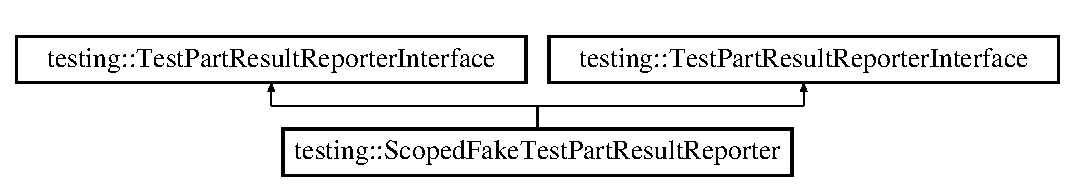
\includegraphics[height=2.000000cm]{classtesting_1_1_scoped_fake_test_part_result_reporter}
\end{center}
\end{figure}
\subsection*{Public Types}
\begin{DoxyCompactItemize}
\item 
\hypertarget{classtesting_1_1_scoped_fake_test_part_result_reporter_a82f6209b3cf5c4b15ec8bd8041dbc2d5}{}enum {\bfseries Intercept\+Mode} \{ {\bfseries I\+N\+T\+E\+R\+C\+E\+P\+T\+\_\+\+O\+N\+L\+Y\+\_\+\+C\+U\+R\+R\+E\+N\+T\+\_\+\+T\+H\+R\+E\+A\+D}, 
{\bfseries I\+N\+T\+E\+R\+C\+E\+P\+T\+\_\+\+A\+L\+L\+\_\+\+T\+H\+R\+E\+A\+D\+S}, 
{\bfseries I\+N\+T\+E\+R\+C\+E\+P\+T\+\_\+\+O\+N\+L\+Y\+\_\+\+C\+U\+R\+R\+E\+N\+T\+\_\+\+T\+H\+R\+E\+A\+D}, 
{\bfseries I\+N\+T\+E\+R\+C\+E\+P\+T\+\_\+\+A\+L\+L\+\_\+\+T\+H\+R\+E\+A\+D\+S}
 \}\label{classtesting_1_1_scoped_fake_test_part_result_reporter_a82f6209b3cf5c4b15ec8bd8041dbc2d5}

\item 
\hypertarget{classtesting_1_1_scoped_fake_test_part_result_reporter_a82f6209b3cf5c4b15ec8bd8041dbc2d5}{}enum {\bfseries Intercept\+Mode} \{ {\bfseries I\+N\+T\+E\+R\+C\+E\+P\+T\+\_\+\+O\+N\+L\+Y\+\_\+\+C\+U\+R\+R\+E\+N\+T\+\_\+\+T\+H\+R\+E\+A\+D}, 
{\bfseries I\+N\+T\+E\+R\+C\+E\+P\+T\+\_\+\+A\+L\+L\+\_\+\+T\+H\+R\+E\+A\+D\+S}, 
{\bfseries I\+N\+T\+E\+R\+C\+E\+P\+T\+\_\+\+O\+N\+L\+Y\+\_\+\+C\+U\+R\+R\+E\+N\+T\+\_\+\+T\+H\+R\+E\+A\+D}, 
{\bfseries I\+N\+T\+E\+R\+C\+E\+P\+T\+\_\+\+A\+L\+L\+\_\+\+T\+H\+R\+E\+A\+D\+S}
 \}\label{classtesting_1_1_scoped_fake_test_part_result_reporter_a82f6209b3cf5c4b15ec8bd8041dbc2d5}

\end{DoxyCompactItemize}
\subsection*{Public Member Functions}
\begin{DoxyCompactItemize}
\item 
\hypertarget{classtesting_1_1_scoped_fake_test_part_result_reporter_aa0100ecf4799fb51d45167be6a5de1d5}{}{\bfseries Scoped\+Fake\+Test\+Part\+Result\+Reporter} (\hyperlink{classtesting_1_1_test_part_result_array}{Test\+Part\+Result\+Array} $\ast$result)\label{classtesting_1_1_scoped_fake_test_part_result_reporter_aa0100ecf4799fb51d45167be6a5de1d5}

\item 
\hypertarget{classtesting_1_1_scoped_fake_test_part_result_reporter_a57cbc09ed48627c8a73e622618dc4b4f}{}{\bfseries Scoped\+Fake\+Test\+Part\+Result\+Reporter} (Intercept\+Mode intercept\+\_\+mode, \hyperlink{classtesting_1_1_test_part_result_array}{Test\+Part\+Result\+Array} $\ast$result)\label{classtesting_1_1_scoped_fake_test_part_result_reporter_a57cbc09ed48627c8a73e622618dc4b4f}

\item 
\hypertarget{classtesting_1_1_scoped_fake_test_part_result_reporter_a3bc6cb939cbc3db71ece8846e6bafe00}{}virtual void {\bfseries Report\+Test\+Part\+Result} (const \hyperlink{classtesting_1_1_test_part_result}{Test\+Part\+Result} \&result)\label{classtesting_1_1_scoped_fake_test_part_result_reporter_a3bc6cb939cbc3db71ece8846e6bafe00}

\item 
\hypertarget{classtesting_1_1_scoped_fake_test_part_result_reporter_aa0100ecf4799fb51d45167be6a5de1d5}{}{\bfseries Scoped\+Fake\+Test\+Part\+Result\+Reporter} (\hyperlink{classtesting_1_1_test_part_result_array}{Test\+Part\+Result\+Array} $\ast$result)\label{classtesting_1_1_scoped_fake_test_part_result_reporter_aa0100ecf4799fb51d45167be6a5de1d5}

\item 
\hypertarget{classtesting_1_1_scoped_fake_test_part_result_reporter_a57cbc09ed48627c8a73e622618dc4b4f}{}{\bfseries Scoped\+Fake\+Test\+Part\+Result\+Reporter} (Intercept\+Mode intercept\+\_\+mode, \hyperlink{classtesting_1_1_test_part_result_array}{Test\+Part\+Result\+Array} $\ast$result)\label{classtesting_1_1_scoped_fake_test_part_result_reporter_a57cbc09ed48627c8a73e622618dc4b4f}

\item 
\hypertarget{classtesting_1_1_scoped_fake_test_part_result_reporter_a3bc6cb939cbc3db71ece8846e6bafe00}{}virtual void {\bfseries Report\+Test\+Part\+Result} (const \hyperlink{classtesting_1_1_test_part_result}{Test\+Part\+Result} \&result)\label{classtesting_1_1_scoped_fake_test_part_result_reporter_a3bc6cb939cbc3db71ece8846e6bafe00}

\end{DoxyCompactItemize}


The documentation for this class was generated from the following file\+:\begin{DoxyCompactItemize}
\item 
deps/win32/debug/include/gtest/gtest-\/spi.\+h\end{DoxyCompactItemize}

\hypertarget{classtesting_1_1internal_1_1_scoped_trace}{}\section{testing\+:\+:internal\+:\+:Scoped\+Trace Class Reference}
\label{classtesting_1_1internal_1_1_scoped_trace}\index{testing\+::internal\+::\+Scoped\+Trace@{testing\+::internal\+::\+Scoped\+Trace}}
\subsection*{Public Member Functions}
\begin{DoxyCompactItemize}
\item 
\hypertarget{classtesting_1_1internal_1_1_scoped_trace_ab965d7010bbbc82c1bef6ebf8748bede}{}{\bfseries Scoped\+Trace} (const char $\ast$file, int line, const \hyperlink{classtesting_1_1_message}{Message} \&message)\label{classtesting_1_1internal_1_1_scoped_trace_ab965d7010bbbc82c1bef6ebf8748bede}

\item 
\hypertarget{classtesting_1_1internal_1_1_scoped_trace_ab965d7010bbbc82c1bef6ebf8748bede}{}{\bfseries Scoped\+Trace} (const char $\ast$file, int line, const \hyperlink{classtesting_1_1_message}{Message} \&message)\label{classtesting_1_1internal_1_1_scoped_trace_ab965d7010bbbc82c1bef6ebf8748bede}

\end{DoxyCompactItemize}


The documentation for this class was generated from the following file\+:\begin{DoxyCompactItemize}
\item 
deps/win32/debug/include/gtest/internal/gtest-\/internal.\+h\end{DoxyCompactItemize}

\hypertarget{classtesting_1_1internal_1_1_single_failure_checker}{}\section{testing\+:\+:internal\+:\+:Single\+Failure\+Checker Class Reference}
\label{classtesting_1_1internal_1_1_single_failure_checker}\index{testing\+::internal\+::\+Single\+Failure\+Checker@{testing\+::internal\+::\+Single\+Failure\+Checker}}
\subsection*{Public Member Functions}
\begin{DoxyCompactItemize}
\item 
\hypertarget{classtesting_1_1internal_1_1_single_failure_checker_a6d350d385526c97c9982e928f5f8fb56}{}{\bfseries Single\+Failure\+Checker} (const \hyperlink{classtesting_1_1_test_part_result_array}{Test\+Part\+Result\+Array} $\ast$results, Test\+Part\+Result\+::\+Type type, const string \&substr)\label{classtesting_1_1internal_1_1_single_failure_checker_a6d350d385526c97c9982e928f5f8fb56}

\item 
\hypertarget{classtesting_1_1internal_1_1_single_failure_checker_a6d350d385526c97c9982e928f5f8fb56}{}{\bfseries Single\+Failure\+Checker} (const \hyperlink{classtesting_1_1_test_part_result_array}{Test\+Part\+Result\+Array} $\ast$results, Test\+Part\+Result\+::\+Type type, const string \&substr)\label{classtesting_1_1internal_1_1_single_failure_checker_a6d350d385526c97c9982e928f5f8fb56}

\end{DoxyCompactItemize}


The documentation for this class was generated from the following file\+:\begin{DoxyCompactItemize}
\item 
deps/win32/debug/include/gtest/gtest-\/spi.\+h\end{DoxyCompactItemize}

\hypertarget{structtesting_1_1internal_1_1_static_assert_type_eq_helper}{}\section{testing\+:\+:internal\+:\+:Static\+Assert\+Type\+Eq\+Helper$<$ T1, T2 $>$ Struct Template Reference}
\label{structtesting_1_1internal_1_1_static_assert_type_eq_helper}\index{testing\+::internal\+::\+Static\+Assert\+Type\+Eq\+Helper$<$ T1, T2 $>$@{testing\+::internal\+::\+Static\+Assert\+Type\+Eq\+Helper$<$ T1, T2 $>$}}


The documentation for this struct was generated from the following file\+:\begin{DoxyCompactItemize}
\item 
deps/win32/debug/include/gtest/internal/gtest-\/port.\+h\end{DoxyCompactItemize}

\hypertarget{structtesting_1_1internal_1_1_static_assert_type_eq_helper_3_01_t_00_01_t_01_4}{}\section{testing\+:\+:internal\+:\+:Static\+Assert\+Type\+Eq\+Helper$<$ T, T $>$ Struct Template Reference}
\label{structtesting_1_1internal_1_1_static_assert_type_eq_helper_3_01_t_00_01_t_01_4}\index{testing\+::internal\+::\+Static\+Assert\+Type\+Eq\+Helper$<$ T, T $>$@{testing\+::internal\+::\+Static\+Assert\+Type\+Eq\+Helper$<$ T, T $>$}}


The documentation for this struct was generated from the following file\+:\begin{DoxyCompactItemize}
\item 
deps/win32/debug/include/gtest/internal/gtest-\/port.\+h\end{DoxyCompactItemize}

\hypertarget{classtesting_1_1internal_1_1_string}{}\section{testing\+:\+:internal\+:\+:String Class Reference}
\label{classtesting_1_1internal_1_1_string}\index{testing\+::internal\+::\+String@{testing\+::internal\+::\+String}}
\subsection*{Static Public Member Functions}
\begin{DoxyCompactItemize}
\item 
\hypertarget{classtesting_1_1internal_1_1_string_a8bce6b1281ae3d2f9061b920aa78aca0}{}static const char $\ast$ {\bfseries Clone\+C\+String} (const char $\ast$c\+\_\+str)\label{classtesting_1_1internal_1_1_string_a8bce6b1281ae3d2f9061b920aa78aca0}

\item 
\hypertarget{classtesting_1_1internal_1_1_string_a06919f642bd47f0593196b460d352f24}{}static bool {\bfseries C\+String\+Equals} (const char $\ast$lhs, const char $\ast$rhs)\label{classtesting_1_1internal_1_1_string_a06919f642bd47f0593196b460d352f24}

\item 
\hypertarget{classtesting_1_1internal_1_1_string_acbf0511e9ae5009f42de77e565f6ba61}{}static std\+::string {\bfseries Show\+Wide\+C\+String} (const wchar\+\_\+t $\ast$wide\+\_\+c\+\_\+str)\label{classtesting_1_1internal_1_1_string_acbf0511e9ae5009f42de77e565f6ba61}

\item 
\hypertarget{classtesting_1_1internal_1_1_string_a4f5e053907ebced07fe0dc52dd2d1e85}{}static bool {\bfseries Wide\+C\+String\+Equals} (const wchar\+\_\+t $\ast$lhs, const wchar\+\_\+t $\ast$rhs)\label{classtesting_1_1internal_1_1_string_a4f5e053907ebced07fe0dc52dd2d1e85}

\item 
\hypertarget{classtesting_1_1internal_1_1_string_a7ce24c41c67b928fe89434d3571c988c}{}static bool {\bfseries Case\+Insensitive\+C\+String\+Equals} (const char $\ast$lhs, const char $\ast$rhs)\label{classtesting_1_1internal_1_1_string_a7ce24c41c67b928fe89434d3571c988c}

\item 
\hypertarget{classtesting_1_1internal_1_1_string_a0a67eac434fa7800640c9d56cb91e105}{}static bool {\bfseries Case\+Insensitive\+Wide\+C\+String\+Equals} (const wchar\+\_\+t $\ast$lhs, const wchar\+\_\+t $\ast$rhs)\label{classtesting_1_1internal_1_1_string_a0a67eac434fa7800640c9d56cb91e105}

\item 
\hypertarget{classtesting_1_1internal_1_1_string_a3de1df085eddc89ef3f3833c67aee3fe}{}static bool {\bfseries Ends\+With\+Case\+Insensitive} (const std\+::string \&str, const std\+::string \&suffix)\label{classtesting_1_1internal_1_1_string_a3de1df085eddc89ef3f3833c67aee3fe}

\item 
\hypertarget{classtesting_1_1internal_1_1_string_a51cab855f7ec6091e5886b6be5598ca2}{}static std\+::string {\bfseries Format\+Int\+Width2} (int value)\label{classtesting_1_1internal_1_1_string_a51cab855f7ec6091e5886b6be5598ca2}

\item 
\hypertarget{classtesting_1_1internal_1_1_string_a7bedf4780e0c938d203b73ddb17ff490}{}static std\+::string {\bfseries Format\+Hex\+Int} (int value)\label{classtesting_1_1internal_1_1_string_a7bedf4780e0c938d203b73ddb17ff490}

\item 
\hypertarget{classtesting_1_1internal_1_1_string_ab3555eeb6abe4b7c6f63d865af10379d}{}static std\+::string {\bfseries Format\+Byte} (unsigned char value)\label{classtesting_1_1internal_1_1_string_ab3555eeb6abe4b7c6f63d865af10379d}

\item 
\hypertarget{classtesting_1_1internal_1_1_string_a8bce6b1281ae3d2f9061b920aa78aca0}{}static const char $\ast$ {\bfseries Clone\+C\+String} (const char $\ast$c\+\_\+str)\label{classtesting_1_1internal_1_1_string_a8bce6b1281ae3d2f9061b920aa78aca0}

\item 
\hypertarget{classtesting_1_1internal_1_1_string_a06919f642bd47f0593196b460d352f24}{}static bool {\bfseries C\+String\+Equals} (const char $\ast$lhs, const char $\ast$rhs)\label{classtesting_1_1internal_1_1_string_a06919f642bd47f0593196b460d352f24}

\item 
\hypertarget{classtesting_1_1internal_1_1_string_acbf0511e9ae5009f42de77e565f6ba61}{}static std\+::string {\bfseries Show\+Wide\+C\+String} (const wchar\+\_\+t $\ast$wide\+\_\+c\+\_\+str)\label{classtesting_1_1internal_1_1_string_acbf0511e9ae5009f42de77e565f6ba61}

\item 
\hypertarget{classtesting_1_1internal_1_1_string_a4f5e053907ebced07fe0dc52dd2d1e85}{}static bool {\bfseries Wide\+C\+String\+Equals} (const wchar\+\_\+t $\ast$lhs, const wchar\+\_\+t $\ast$rhs)\label{classtesting_1_1internal_1_1_string_a4f5e053907ebced07fe0dc52dd2d1e85}

\item 
\hypertarget{classtesting_1_1internal_1_1_string_a7ce24c41c67b928fe89434d3571c988c}{}static bool {\bfseries Case\+Insensitive\+C\+String\+Equals} (const char $\ast$lhs, const char $\ast$rhs)\label{classtesting_1_1internal_1_1_string_a7ce24c41c67b928fe89434d3571c988c}

\item 
\hypertarget{classtesting_1_1internal_1_1_string_a0a67eac434fa7800640c9d56cb91e105}{}static bool {\bfseries Case\+Insensitive\+Wide\+C\+String\+Equals} (const wchar\+\_\+t $\ast$lhs, const wchar\+\_\+t $\ast$rhs)\label{classtesting_1_1internal_1_1_string_a0a67eac434fa7800640c9d56cb91e105}

\item 
\hypertarget{classtesting_1_1internal_1_1_string_a3de1df085eddc89ef3f3833c67aee3fe}{}static bool {\bfseries Ends\+With\+Case\+Insensitive} (const std\+::string \&str, const std\+::string \&suffix)\label{classtesting_1_1internal_1_1_string_a3de1df085eddc89ef3f3833c67aee3fe}

\item 
\hypertarget{classtesting_1_1internal_1_1_string_a51cab855f7ec6091e5886b6be5598ca2}{}static std\+::string {\bfseries Format\+Int\+Width2} (int value)\label{classtesting_1_1internal_1_1_string_a51cab855f7ec6091e5886b6be5598ca2}

\item 
\hypertarget{classtesting_1_1internal_1_1_string_a7bedf4780e0c938d203b73ddb17ff490}{}static std\+::string {\bfseries Format\+Hex\+Int} (int value)\label{classtesting_1_1internal_1_1_string_a7bedf4780e0c938d203b73ddb17ff490}

\item 
\hypertarget{classtesting_1_1internal_1_1_string_ab3555eeb6abe4b7c6f63d865af10379d}{}static std\+::string {\bfseries Format\+Byte} (unsigned char value)\label{classtesting_1_1internal_1_1_string_ab3555eeb6abe4b7c6f63d865af10379d}

\end{DoxyCompactItemize}


The documentation for this class was generated from the following file\+:\begin{DoxyCompactItemize}
\item 
deps/win32/debug/include/gtest/internal/gtest-\/string.\+h\end{DoxyCompactItemize}

\hypertarget{classtesting_1_1_test}{}\section{testing\+:\+:Test Class Reference}
\label{classtesting_1_1_test}\index{testing\+::\+Test@{testing\+::\+Test}}
Inheritance diagram for testing\+:\+:Test\+:\begin{figure}[H]
\begin{center}
\leavevmode
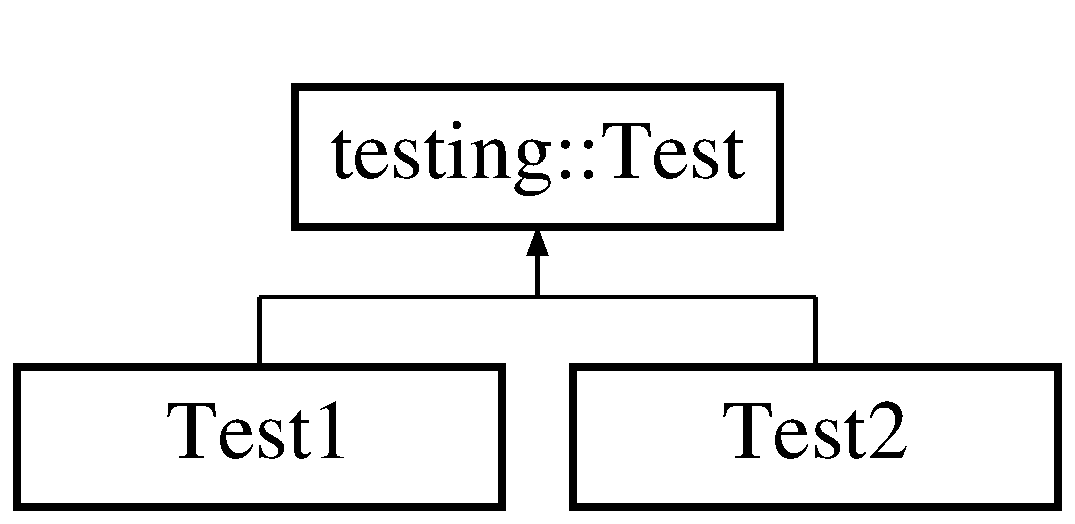
\includegraphics[height=2.000000cm]{classtesting_1_1_test}
\end{center}
\end{figure}
\subsection*{Public Types}
\begin{DoxyCompactItemize}
\item 
\hypertarget{classtesting_1_1_test_a5f2a051d1d99c9b784c666c586186cf9}{}typedef internal\+::\+Set\+Up\+Test\+Case\+Func {\bfseries Set\+Up\+Test\+Case\+Func}\label{classtesting_1_1_test_a5f2a051d1d99c9b784c666c586186cf9}

\item 
\hypertarget{classtesting_1_1_test_aa0f532e93b9f3500144c53f31466976c}{}typedef internal\+::\+Tear\+Down\+Test\+Case\+Func {\bfseries Tear\+Down\+Test\+Case\+Func}\label{classtesting_1_1_test_aa0f532e93b9f3500144c53f31466976c}

\item 
\hypertarget{classtesting_1_1_test_a5f2a051d1d99c9b784c666c586186cf9}{}typedef internal\+::\+Set\+Up\+Test\+Case\+Func {\bfseries Set\+Up\+Test\+Case\+Func}\label{classtesting_1_1_test_a5f2a051d1d99c9b784c666c586186cf9}

\item 
\hypertarget{classtesting_1_1_test_aa0f532e93b9f3500144c53f31466976c}{}typedef internal\+::\+Tear\+Down\+Test\+Case\+Func {\bfseries Tear\+Down\+Test\+Case\+Func}\label{classtesting_1_1_test_aa0f532e93b9f3500144c53f31466976c}

\end{DoxyCompactItemize}
\subsection*{Static Public Member Functions}
\begin{DoxyCompactItemize}
\item 
\hypertarget{classtesting_1_1_test_a5ccbac42fee8c5b00b0bfe89b6c49d79}{}static void {\bfseries Set\+Up\+Test\+Case} ()\label{classtesting_1_1_test_a5ccbac42fee8c5b00b0bfe89b6c49d79}

\item 
\hypertarget{classtesting_1_1_test_af374706cbaf0ffc460f4fd04e7c150f1}{}static void {\bfseries Tear\+Down\+Test\+Case} ()\label{classtesting_1_1_test_af374706cbaf0ffc460f4fd04e7c150f1}

\item 
\hypertarget{classtesting_1_1_test_a0a89846458f0e8ed1c9457c957e8182a}{}static bool {\bfseries Has\+Fatal\+Failure} ()\label{classtesting_1_1_test_a0a89846458f0e8ed1c9457c957e8182a}

\item 
\hypertarget{classtesting_1_1_test_a07e896f1b1836f8ac075c26d7b7c9fb8}{}static bool {\bfseries Has\+Nonfatal\+Failure} ()\label{classtesting_1_1_test_a07e896f1b1836f8ac075c26d7b7c9fb8}

\item 
\hypertarget{classtesting_1_1_test_a7a00be7dd0a6bfdc8d47a1b784623613}{}static bool {\bfseries Has\+Failure} ()\label{classtesting_1_1_test_a7a00be7dd0a6bfdc8d47a1b784623613}

\item 
\hypertarget{classtesting_1_1_test_ae0448aec9e389fab70f6a75a59ff6aa2}{}static void {\bfseries Record\+Property} (const std\+::string \&key, const std\+::string \&value)\label{classtesting_1_1_test_ae0448aec9e389fab70f6a75a59ff6aa2}

\item 
\hypertarget{classtesting_1_1_test_af602903efb17730b977304fc56500881}{}static void {\bfseries Record\+Property} (const std\+::string \&key, int value)\label{classtesting_1_1_test_af602903efb17730b977304fc56500881}

\item 
\hypertarget{classtesting_1_1_test_a5ccbac42fee8c5b00b0bfe89b6c49d79}{}static void {\bfseries Set\+Up\+Test\+Case} ()\label{classtesting_1_1_test_a5ccbac42fee8c5b00b0bfe89b6c49d79}

\item 
\hypertarget{classtesting_1_1_test_af374706cbaf0ffc460f4fd04e7c150f1}{}static void {\bfseries Tear\+Down\+Test\+Case} ()\label{classtesting_1_1_test_af374706cbaf0ffc460f4fd04e7c150f1}

\item 
\hypertarget{classtesting_1_1_test_a0a89846458f0e8ed1c9457c957e8182a}{}static bool {\bfseries Has\+Fatal\+Failure} ()\label{classtesting_1_1_test_a0a89846458f0e8ed1c9457c957e8182a}

\item 
\hypertarget{classtesting_1_1_test_a07e896f1b1836f8ac075c26d7b7c9fb8}{}static bool {\bfseries Has\+Nonfatal\+Failure} ()\label{classtesting_1_1_test_a07e896f1b1836f8ac075c26d7b7c9fb8}

\item 
\hypertarget{classtesting_1_1_test_a7a00be7dd0a6bfdc8d47a1b784623613}{}static bool {\bfseries Has\+Failure} ()\label{classtesting_1_1_test_a7a00be7dd0a6bfdc8d47a1b784623613}

\item 
\hypertarget{classtesting_1_1_test_ae0448aec9e389fab70f6a75a59ff6aa2}{}static void {\bfseries Record\+Property} (const std\+::string \&key, const std\+::string \&value)\label{classtesting_1_1_test_ae0448aec9e389fab70f6a75a59ff6aa2}

\item 
\hypertarget{classtesting_1_1_test_af602903efb17730b977304fc56500881}{}static void {\bfseries Record\+Property} (const std\+::string \&key, int value)\label{classtesting_1_1_test_af602903efb17730b977304fc56500881}

\end{DoxyCompactItemize}
\subsection*{Protected Member Functions}
\begin{DoxyCompactItemize}
\item 
\hypertarget{classtesting_1_1_test_a8b38992669fb844864807cf32e416853}{}virtual void {\bfseries Set\+Up} ()\label{classtesting_1_1_test_a8b38992669fb844864807cf32e416853}

\item 
\hypertarget{classtesting_1_1_test_aab3c02c9f81afe1357adfc45afccd474}{}virtual void {\bfseries Tear\+Down} ()\label{classtesting_1_1_test_aab3c02c9f81afe1357adfc45afccd474}

\item 
\hypertarget{classtesting_1_1_test_a8b38992669fb844864807cf32e416853}{}virtual void {\bfseries Set\+Up} ()\label{classtesting_1_1_test_a8b38992669fb844864807cf32e416853}

\item 
\hypertarget{classtesting_1_1_test_aab3c02c9f81afe1357adfc45afccd474}{}virtual void {\bfseries Tear\+Down} ()\label{classtesting_1_1_test_aab3c02c9f81afe1357adfc45afccd474}

\end{DoxyCompactItemize}
\subsection*{Friends}
\begin{DoxyCompactItemize}
\item 
\hypertarget{classtesting_1_1_test_aed3c96e2bd5a46339c1cbe49a4a233ee}{}class {\bfseries Test\+Info}\label{classtesting_1_1_test_aed3c96e2bd5a46339c1cbe49a4a233ee}

\end{DoxyCompactItemize}


The documentation for this class was generated from the following file\+:\begin{DoxyCompactItemize}
\item 
deps/win32/debug/include/gtest/gtest.\+h\end{DoxyCompactItemize}

\hypertarget{class_test1}{}\section{Test1 Class Reference}
\label{class_test1}\index{Test1@{Test1}}
Inheritance diagram for Test1\+:\begin{figure}[H]
\begin{center}
\leavevmode
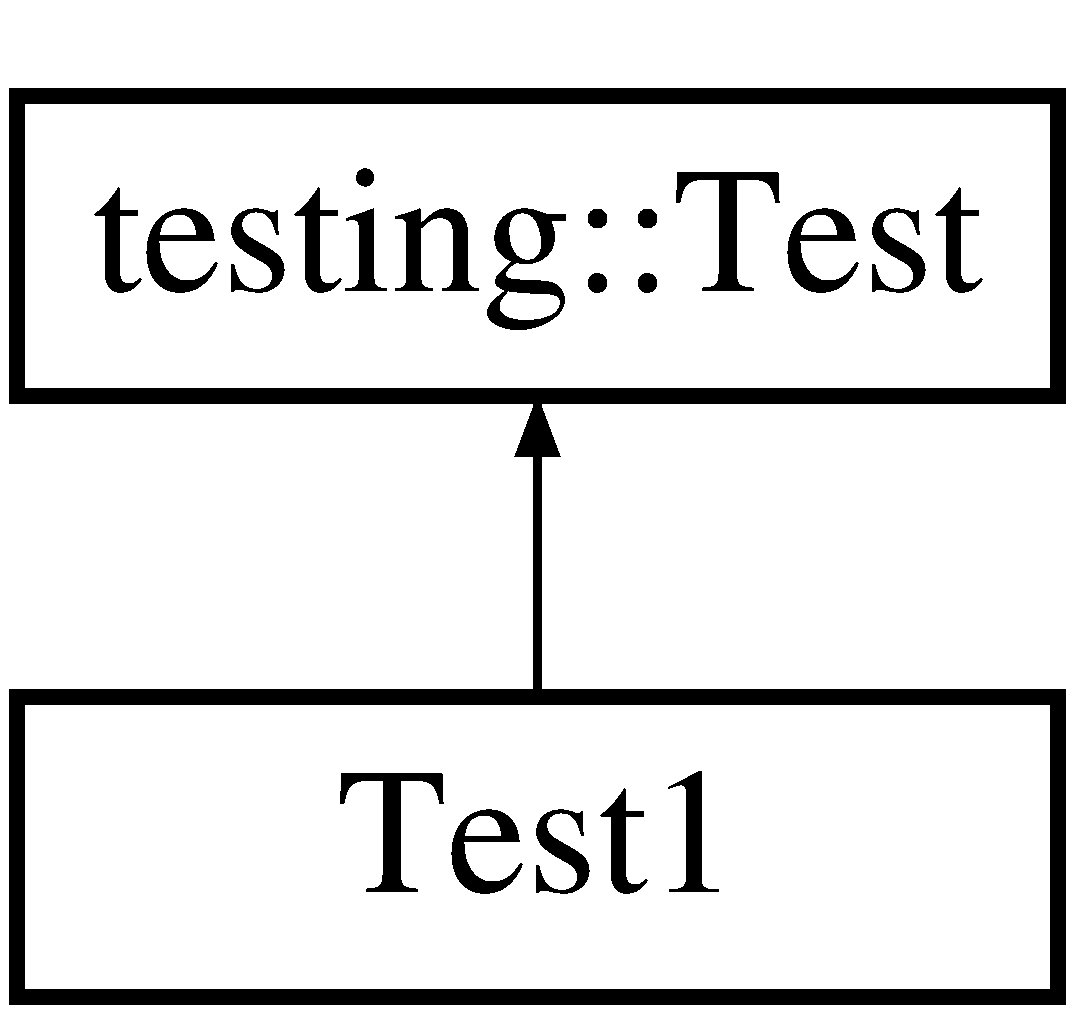
\includegraphics[height=2.000000cm]{class_test1}
\end{center}
\end{figure}
\subsection*{Static Public Member Functions}
\begin{DoxyCompactItemize}
\item 
\hypertarget{class_test1_a7d36718d0baec0b5a96b33dadee695c2}{}static void {\bfseries init} ()\label{class_test1_a7d36718d0baec0b5a96b33dadee695c2}

\item 
\hypertarget{class_test1_ab574a5869ab0af072f5047fa396a5af9}{}static void {\bfseries display} ()\label{class_test1_ab574a5869ab0af072f5047fa396a5af9}

\end{DoxyCompactItemize}
\subsection*{Static Public Attributes}
\begin{DoxyCompactItemize}
\item 
\hypertarget{class_test1_aad528bbab0c48086d4bf59100d36e0b1}{}static G\+Luint $\ast$ {\bfseries V\+A\+O} = new G\+Luint\mbox{[}1\mbox{]}\label{class_test1_aad528bbab0c48086d4bf59100d36e0b1}

\item 
\hypertarget{class_test1_ab027878a7b35af15e679b223c0bdf64d}{}static G\+Luint $\ast$ {\bfseries V\+B\+O} = new G\+Luint\mbox{[}1\mbox{]}\label{class_test1_ab027878a7b35af15e679b223c0bdf64d}

\end{DoxyCompactItemize}
\subsection*{Additional Inherited Members}


The documentation for this class was generated from the following files\+:\begin{DoxyCompactItemize}
\item 
src/test/opengl\+\_\+test.\+h\item 
src/test/opengl\+\_\+test.\+cpp\end{DoxyCompactItemize}

\hypertarget{class_test2}{}\section{Test2 Class Reference}
\label{class_test2}\index{Test2@{Test2}}
Inheritance diagram for Test2\+:\begin{figure}[H]
\begin{center}
\leavevmode
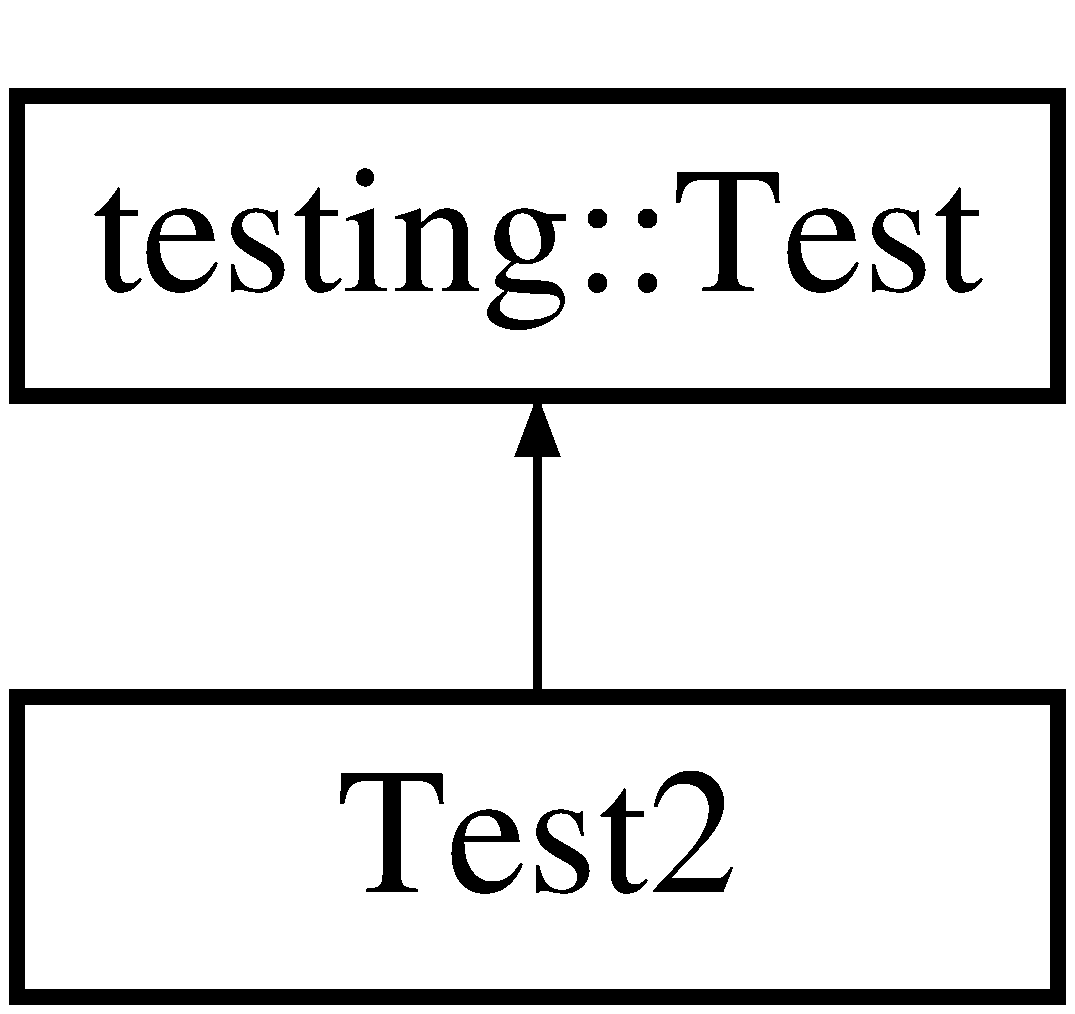
\includegraphics[height=2.000000cm]{class_test2}
\end{center}
\end{figure}
\subsection*{Static Public Member Functions}
\begin{DoxyCompactItemize}
\item 
\hypertarget{class_test2_afa0c32c3dd75a5645c9ce931c5cf316f}{}static void {\bfseries init} ()\label{class_test2_afa0c32c3dd75a5645c9ce931c5cf316f}

\item 
\hypertarget{class_test2_a7455e00e9ada90a99f15b0a938fa96c0}{}static void {\bfseries display} ()\label{class_test2_a7455e00e9ada90a99f15b0a938fa96c0}

\end{DoxyCompactItemize}
\subsection*{Static Public Attributes}
\begin{DoxyCompactItemize}
\item 
\hypertarget{class_test2_abd780937ac6b4ace7cd10db14e143b40}{}static G\+Luint {\bfseries vao} \mbox{[}$\,$\mbox{]}\label{class_test2_abd780937ac6b4ace7cd10db14e143b40}

\item 
\hypertarget{class_test2_ac4b0615887205ec2597f17b1eb28c259}{}static G\+Luint {\bfseries vbo} \mbox{[}$\,$\mbox{]}\label{class_test2_ac4b0615887205ec2597f17b1eb28c259}

\item 
\hypertarget{class_test2_a0f31cd9f0934e6463deb78b17e2f9d8d}{}static G\+Luint {\bfseries ebo} \mbox{[}$\,$\mbox{]}\label{class_test2_a0f31cd9f0934e6463deb78b17e2f9d8d}

\end{DoxyCompactItemize}
\subsection*{Additional Inherited Members}


The documentation for this class was generated from the following files\+:\begin{DoxyCompactItemize}
\item 
src/test/opengl\+\_\+test.\+h\item 
src/test/opengl\+\_\+test.\+cpp\end{DoxyCompactItemize}

\hypertarget{classtesting_1_1_test_case}{}\section{testing\+:\+:Test\+Case Class Reference}
\label{classtesting_1_1_test_case}\index{testing\+::\+Test\+Case@{testing\+::\+Test\+Case}}
\subsection*{Public Member Functions}
\begin{DoxyCompactItemize}
\item 
\hypertarget{classtesting_1_1_test_case_a8a43b04703bfc7d56597fcb9b76ffbf5}{}{\bfseries Test\+Case} (const char $\ast$name, const char $\ast$a\+\_\+type\+\_\+param, Test\+::\+Set\+Up\+Test\+Case\+Func set\+\_\+up\+\_\+tc, Test\+::\+Tear\+Down\+Test\+Case\+Func tear\+\_\+down\+\_\+tc)\label{classtesting_1_1_test_case_a8a43b04703bfc7d56597fcb9b76ffbf5}

\item 
\hypertarget{classtesting_1_1_test_case_af4dfd4ece8e66520a30e6a9fbd9d43aa}{}const char $\ast$ {\bfseries name} () const \label{classtesting_1_1_test_case_af4dfd4ece8e66520a30e6a9fbd9d43aa}

\item 
\hypertarget{classtesting_1_1_test_case_a2052c095bc6ac9c0ab1cae6f0e2d9fc9}{}const char $\ast$ {\bfseries type\+\_\+param} () const \label{classtesting_1_1_test_case_a2052c095bc6ac9c0ab1cae6f0e2d9fc9}

\item 
\hypertarget{classtesting_1_1_test_case_a0e49de754452943d88e3083e6cdded00}{}bool {\bfseries should\+\_\+run} () const \label{classtesting_1_1_test_case_a0e49de754452943d88e3083e6cdded00}

\item 
\hypertarget{classtesting_1_1_test_case_a8fb3974ccb5242ad9d1d633d53c0f730}{}int {\bfseries successful\+\_\+test\+\_\+count} () const \label{classtesting_1_1_test_case_a8fb3974ccb5242ad9d1d633d53c0f730}

\item 
\hypertarget{classtesting_1_1_test_case_ae74e7a2e75d07f9feca2c3384604cb01}{}int {\bfseries failed\+\_\+test\+\_\+count} () const \label{classtesting_1_1_test_case_ae74e7a2e75d07f9feca2c3384604cb01}

\item 
\hypertarget{classtesting_1_1_test_case_a4ec19c0058282562c0cc2c0e87d4b211}{}int {\bfseries reportable\+\_\+disabled\+\_\+test\+\_\+count} () const \label{classtesting_1_1_test_case_a4ec19c0058282562c0cc2c0e87d4b211}

\item 
\hypertarget{classtesting_1_1_test_case_ac1e3cd2b598f19ce10e42b3421508a9e}{}int {\bfseries disabled\+\_\+test\+\_\+count} () const \label{classtesting_1_1_test_case_ac1e3cd2b598f19ce10e42b3421508a9e}

\item 
\hypertarget{classtesting_1_1_test_case_a7693150fa71d460a19b291ed6f5c18bd}{}int {\bfseries reportable\+\_\+test\+\_\+count} () const \label{classtesting_1_1_test_case_a7693150fa71d460a19b291ed6f5c18bd}

\item 
\hypertarget{classtesting_1_1_test_case_a47de0cf87858370388275c9d995f1ff4}{}int {\bfseries test\+\_\+to\+\_\+run\+\_\+count} () const \label{classtesting_1_1_test_case_a47de0cf87858370388275c9d995f1ff4}

\item 
\hypertarget{classtesting_1_1_test_case_ac7b2ed22822735b7b9ae2740162332c9}{}int {\bfseries total\+\_\+test\+\_\+count} () const \label{classtesting_1_1_test_case_ac7b2ed22822735b7b9ae2740162332c9}

\item 
\hypertarget{classtesting_1_1_test_case_ad093a04334d7eb8d707a7f1a321b040f}{}bool {\bfseries Passed} () const \label{classtesting_1_1_test_case_ad093a04334d7eb8d707a7f1a321b040f}

\item 
\hypertarget{classtesting_1_1_test_case_a5c0922d310f860e78cca7e215f2fa0e4}{}bool {\bfseries Failed} () const \label{classtesting_1_1_test_case_a5c0922d310f860e78cca7e215f2fa0e4}

\item 
\hypertarget{classtesting_1_1_test_case_a80f163d2826ba8586fffb41e8d686727}{}Time\+In\+Millis {\bfseries elapsed\+\_\+time} () const \label{classtesting_1_1_test_case_a80f163d2826ba8586fffb41e8d686727}

\item 
\hypertarget{classtesting_1_1_test_case_a17dfa2a9fde64f5add3615e9426e81e1}{}const \hyperlink{classtesting_1_1_test_info}{Test\+Info} $\ast$ {\bfseries Get\+Test\+Info} (int i) const \label{classtesting_1_1_test_case_a17dfa2a9fde64f5add3615e9426e81e1}

\item 
\hypertarget{classtesting_1_1_test_case_a3993481a8f0c2253653b5e1ec5934432}{}const \hyperlink{classtesting_1_1_test_result}{Test\+Result} \& {\bfseries ad\+\_\+hoc\+\_\+test\+\_\+result} () const \label{classtesting_1_1_test_case_a3993481a8f0c2253653b5e1ec5934432}

\item 
\hypertarget{classtesting_1_1_test_case_a8a43b04703bfc7d56597fcb9b76ffbf5}{}{\bfseries Test\+Case} (const char $\ast$name, const char $\ast$a\+\_\+type\+\_\+param, Test\+::\+Set\+Up\+Test\+Case\+Func set\+\_\+up\+\_\+tc, Test\+::\+Tear\+Down\+Test\+Case\+Func tear\+\_\+down\+\_\+tc)\label{classtesting_1_1_test_case_a8a43b04703bfc7d56597fcb9b76ffbf5}

\item 
\hypertarget{classtesting_1_1_test_case_af4dfd4ece8e66520a30e6a9fbd9d43aa}{}const char $\ast$ {\bfseries name} () const \label{classtesting_1_1_test_case_af4dfd4ece8e66520a30e6a9fbd9d43aa}

\item 
\hypertarget{classtesting_1_1_test_case_a2052c095bc6ac9c0ab1cae6f0e2d9fc9}{}const char $\ast$ {\bfseries type\+\_\+param} () const \label{classtesting_1_1_test_case_a2052c095bc6ac9c0ab1cae6f0e2d9fc9}

\item 
\hypertarget{classtesting_1_1_test_case_a0e49de754452943d88e3083e6cdded00}{}bool {\bfseries should\+\_\+run} () const \label{classtesting_1_1_test_case_a0e49de754452943d88e3083e6cdded00}

\item 
\hypertarget{classtesting_1_1_test_case_a8fb3974ccb5242ad9d1d633d53c0f730}{}int {\bfseries successful\+\_\+test\+\_\+count} () const \label{classtesting_1_1_test_case_a8fb3974ccb5242ad9d1d633d53c0f730}

\item 
\hypertarget{classtesting_1_1_test_case_ae74e7a2e75d07f9feca2c3384604cb01}{}int {\bfseries failed\+\_\+test\+\_\+count} () const \label{classtesting_1_1_test_case_ae74e7a2e75d07f9feca2c3384604cb01}

\item 
\hypertarget{classtesting_1_1_test_case_a4ec19c0058282562c0cc2c0e87d4b211}{}int {\bfseries reportable\+\_\+disabled\+\_\+test\+\_\+count} () const \label{classtesting_1_1_test_case_a4ec19c0058282562c0cc2c0e87d4b211}

\item 
\hypertarget{classtesting_1_1_test_case_ac1e3cd2b598f19ce10e42b3421508a9e}{}int {\bfseries disabled\+\_\+test\+\_\+count} () const \label{classtesting_1_1_test_case_ac1e3cd2b598f19ce10e42b3421508a9e}

\item 
\hypertarget{classtesting_1_1_test_case_a7693150fa71d460a19b291ed6f5c18bd}{}int {\bfseries reportable\+\_\+test\+\_\+count} () const \label{classtesting_1_1_test_case_a7693150fa71d460a19b291ed6f5c18bd}

\item 
\hypertarget{classtesting_1_1_test_case_a47de0cf87858370388275c9d995f1ff4}{}int {\bfseries test\+\_\+to\+\_\+run\+\_\+count} () const \label{classtesting_1_1_test_case_a47de0cf87858370388275c9d995f1ff4}

\item 
\hypertarget{classtesting_1_1_test_case_ac7b2ed22822735b7b9ae2740162332c9}{}int {\bfseries total\+\_\+test\+\_\+count} () const \label{classtesting_1_1_test_case_ac7b2ed22822735b7b9ae2740162332c9}

\item 
\hypertarget{classtesting_1_1_test_case_ad093a04334d7eb8d707a7f1a321b040f}{}bool {\bfseries Passed} () const \label{classtesting_1_1_test_case_ad093a04334d7eb8d707a7f1a321b040f}

\item 
\hypertarget{classtesting_1_1_test_case_a5c0922d310f860e78cca7e215f2fa0e4}{}bool {\bfseries Failed} () const \label{classtesting_1_1_test_case_a5c0922d310f860e78cca7e215f2fa0e4}

\item 
\hypertarget{classtesting_1_1_test_case_a80f163d2826ba8586fffb41e8d686727}{}Time\+In\+Millis {\bfseries elapsed\+\_\+time} () const \label{classtesting_1_1_test_case_a80f163d2826ba8586fffb41e8d686727}

\item 
\hypertarget{classtesting_1_1_test_case_a17dfa2a9fde64f5add3615e9426e81e1}{}const \hyperlink{classtesting_1_1_test_info}{Test\+Info} $\ast$ {\bfseries Get\+Test\+Info} (int i) const \label{classtesting_1_1_test_case_a17dfa2a9fde64f5add3615e9426e81e1}

\item 
\hypertarget{classtesting_1_1_test_case_a3993481a8f0c2253653b5e1ec5934432}{}const \hyperlink{classtesting_1_1_test_result}{Test\+Result} \& {\bfseries ad\+\_\+hoc\+\_\+test\+\_\+result} () const \label{classtesting_1_1_test_case_a3993481a8f0c2253653b5e1ec5934432}

\end{DoxyCompactItemize}
\subsection*{Friends}
\begin{DoxyCompactItemize}
\item 
\hypertarget{classtesting_1_1_test_case_ab085d1bf4cff8b1045750706b11f8662}{}class {\bfseries Test}\label{classtesting_1_1_test_case_ab085d1bf4cff8b1045750706b11f8662}

\item 
\hypertarget{classtesting_1_1_test_case_aa684cc13a8f91b00c0c9ce41ec7474eb}{}class {\bfseries internal\+::\+Unit\+Test\+Impl}\label{classtesting_1_1_test_case_aa684cc13a8f91b00c0c9ce41ec7474eb}

\end{DoxyCompactItemize}


The documentation for this class was generated from the following file\+:\begin{DoxyCompactItemize}
\item 
deps/win32/debug/include/gtest/gtest.\+h\end{DoxyCompactItemize}

\hypertarget{classtesting_1_1_test_event_listener}{}\section{testing\+:\+:Test\+Event\+Listener Class Reference}
\label{classtesting_1_1_test_event_listener}\index{testing\+::\+Test\+Event\+Listener@{testing\+::\+Test\+Event\+Listener}}
Inheritance diagram for testing\+:\+:Test\+Event\+Listener\+:\begin{figure}[H]
\begin{center}
\leavevmode
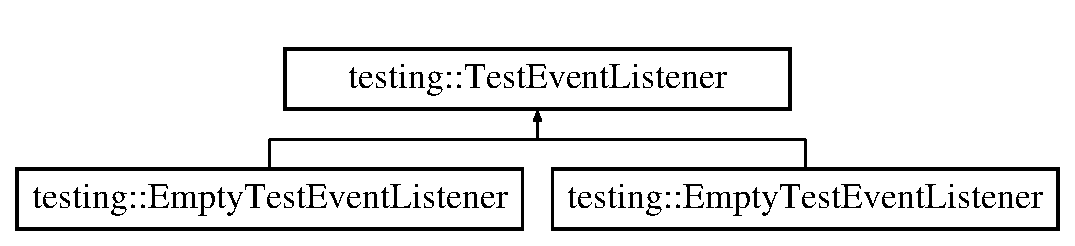
\includegraphics[height=2.000000cm]{classtesting_1_1_test_event_listener}
\end{center}
\end{figure}
\subsection*{Public Member Functions}
\begin{DoxyCompactItemize}
\item 
\hypertarget{classtesting_1_1_test_event_listener_a5f6c84f39851e8a603a2d2e10063816b}{}virtual void {\bfseries On\+Test\+Program\+Start} (const \hyperlink{classtesting_1_1_unit_test}{Unit\+Test} \&unit\+\_\+test)=0\label{classtesting_1_1_test_event_listener_a5f6c84f39851e8a603a2d2e10063816b}

\item 
\hypertarget{classtesting_1_1_test_event_listener_a60cc09b7907cb329d152eb5e7133bdeb}{}virtual void {\bfseries On\+Test\+Iteration\+Start} (const \hyperlink{classtesting_1_1_unit_test}{Unit\+Test} \&unit\+\_\+test, int iteration)=0\label{classtesting_1_1_test_event_listener_a60cc09b7907cb329d152eb5e7133bdeb}

\item 
\hypertarget{classtesting_1_1_test_event_listener_aa6502e534919605be45f26a6daf9a40c}{}virtual void {\bfseries On\+Environments\+Set\+Up\+Start} (const \hyperlink{classtesting_1_1_unit_test}{Unit\+Test} \&unit\+\_\+test)=0\label{classtesting_1_1_test_event_listener_aa6502e534919605be45f26a6daf9a40c}

\item 
\hypertarget{classtesting_1_1_test_event_listener_aaa1021d75f5dbf3f05c829c1cc520341}{}virtual void {\bfseries On\+Environments\+Set\+Up\+End} (const \hyperlink{classtesting_1_1_unit_test}{Unit\+Test} \&unit\+\_\+test)=0\label{classtesting_1_1_test_event_listener_aaa1021d75f5dbf3f05c829c1cc520341}

\item 
\hypertarget{classtesting_1_1_test_event_listener_ab4ed885d63f5bbff8076c1329b3dfe36}{}virtual void {\bfseries On\+Test\+Case\+Start} (const \hyperlink{classtesting_1_1_test_case}{Test\+Case} \&test\+\_\+case)=0\label{classtesting_1_1_test_event_listener_ab4ed885d63f5bbff8076c1329b3dfe36}

\item 
\hypertarget{classtesting_1_1_test_event_listener_ab4f6a0ca16ae75daf385b3b5914e1048}{}virtual void {\bfseries On\+Test\+Start} (const \hyperlink{classtesting_1_1_test_info}{Test\+Info} \&test\+\_\+info)=0\label{classtesting_1_1_test_event_listener_ab4f6a0ca16ae75daf385b3b5914e1048}

\item 
\hypertarget{classtesting_1_1_test_event_listener_a054f8705c883fa120b91473aff38f2ee}{}virtual void {\bfseries On\+Test\+Part\+Result} (const \hyperlink{classtesting_1_1_test_part_result}{Test\+Part\+Result} \&test\+\_\+part\+\_\+result)=0\label{classtesting_1_1_test_event_listener_a054f8705c883fa120b91473aff38f2ee}

\item 
\hypertarget{classtesting_1_1_test_event_listener_abb1c44525ef038500608b5dc2f17099b}{}virtual void {\bfseries On\+Test\+End} (const \hyperlink{classtesting_1_1_test_info}{Test\+Info} \&test\+\_\+info)=0\label{classtesting_1_1_test_event_listener_abb1c44525ef038500608b5dc2f17099b}

\item 
\hypertarget{classtesting_1_1_test_event_listener_ae61985e2ef76ac78379b077be57a9c36}{}virtual void {\bfseries On\+Test\+Case\+End} (const \hyperlink{classtesting_1_1_test_case}{Test\+Case} \&test\+\_\+case)=0\label{classtesting_1_1_test_event_listener_ae61985e2ef76ac78379b077be57a9c36}

\item 
\hypertarget{classtesting_1_1_test_event_listener_a468b5e6701bcb86cb2c956caadbba5e4}{}virtual void {\bfseries On\+Environments\+Tear\+Down\+Start} (const \hyperlink{classtesting_1_1_unit_test}{Unit\+Test} \&unit\+\_\+test)=0\label{classtesting_1_1_test_event_listener_a468b5e6701bcb86cb2c956caadbba5e4}

\item 
\hypertarget{classtesting_1_1_test_event_listener_a9ea04fa7f447865ba76df35e12ba2092}{}virtual void {\bfseries On\+Environments\+Tear\+Down\+End} (const \hyperlink{classtesting_1_1_unit_test}{Unit\+Test} \&unit\+\_\+test)=0\label{classtesting_1_1_test_event_listener_a9ea04fa7f447865ba76df35e12ba2092}

\item 
\hypertarget{classtesting_1_1_test_event_listener_a550fdb3e55726e4cefa09f5697941425}{}virtual void {\bfseries On\+Test\+Iteration\+End} (const \hyperlink{classtesting_1_1_unit_test}{Unit\+Test} \&unit\+\_\+test, int iteration)=0\label{classtesting_1_1_test_event_listener_a550fdb3e55726e4cefa09f5697941425}

\item 
\hypertarget{classtesting_1_1_test_event_listener_ad15b6246d94c268e233487a86463ef3d}{}virtual void {\bfseries On\+Test\+Program\+End} (const \hyperlink{classtesting_1_1_unit_test}{Unit\+Test} \&unit\+\_\+test)=0\label{classtesting_1_1_test_event_listener_ad15b6246d94c268e233487a86463ef3d}

\item 
\hypertarget{classtesting_1_1_test_event_listener_a5f6c84f39851e8a603a2d2e10063816b}{}virtual void {\bfseries On\+Test\+Program\+Start} (const \hyperlink{classtesting_1_1_unit_test}{Unit\+Test} \&unit\+\_\+test)=0\label{classtesting_1_1_test_event_listener_a5f6c84f39851e8a603a2d2e10063816b}

\item 
\hypertarget{classtesting_1_1_test_event_listener_a60cc09b7907cb329d152eb5e7133bdeb}{}virtual void {\bfseries On\+Test\+Iteration\+Start} (const \hyperlink{classtesting_1_1_unit_test}{Unit\+Test} \&unit\+\_\+test, int iteration)=0\label{classtesting_1_1_test_event_listener_a60cc09b7907cb329d152eb5e7133bdeb}

\item 
\hypertarget{classtesting_1_1_test_event_listener_aa6502e534919605be45f26a6daf9a40c}{}virtual void {\bfseries On\+Environments\+Set\+Up\+Start} (const \hyperlink{classtesting_1_1_unit_test}{Unit\+Test} \&unit\+\_\+test)=0\label{classtesting_1_1_test_event_listener_aa6502e534919605be45f26a6daf9a40c}

\item 
\hypertarget{classtesting_1_1_test_event_listener_aaa1021d75f5dbf3f05c829c1cc520341}{}virtual void {\bfseries On\+Environments\+Set\+Up\+End} (const \hyperlink{classtesting_1_1_unit_test}{Unit\+Test} \&unit\+\_\+test)=0\label{classtesting_1_1_test_event_listener_aaa1021d75f5dbf3f05c829c1cc520341}

\item 
\hypertarget{classtesting_1_1_test_event_listener_ab4ed885d63f5bbff8076c1329b3dfe36}{}virtual void {\bfseries On\+Test\+Case\+Start} (const \hyperlink{classtesting_1_1_test_case}{Test\+Case} \&test\+\_\+case)=0\label{classtesting_1_1_test_event_listener_ab4ed885d63f5bbff8076c1329b3dfe36}

\item 
\hypertarget{classtesting_1_1_test_event_listener_ab4f6a0ca16ae75daf385b3b5914e1048}{}virtual void {\bfseries On\+Test\+Start} (const \hyperlink{classtesting_1_1_test_info}{Test\+Info} \&test\+\_\+info)=0\label{classtesting_1_1_test_event_listener_ab4f6a0ca16ae75daf385b3b5914e1048}

\item 
\hypertarget{classtesting_1_1_test_event_listener_a054f8705c883fa120b91473aff38f2ee}{}virtual void {\bfseries On\+Test\+Part\+Result} (const \hyperlink{classtesting_1_1_test_part_result}{Test\+Part\+Result} \&test\+\_\+part\+\_\+result)=0\label{classtesting_1_1_test_event_listener_a054f8705c883fa120b91473aff38f2ee}

\item 
\hypertarget{classtesting_1_1_test_event_listener_abb1c44525ef038500608b5dc2f17099b}{}virtual void {\bfseries On\+Test\+End} (const \hyperlink{classtesting_1_1_test_info}{Test\+Info} \&test\+\_\+info)=0\label{classtesting_1_1_test_event_listener_abb1c44525ef038500608b5dc2f17099b}

\item 
\hypertarget{classtesting_1_1_test_event_listener_ae61985e2ef76ac78379b077be57a9c36}{}virtual void {\bfseries On\+Test\+Case\+End} (const \hyperlink{classtesting_1_1_test_case}{Test\+Case} \&test\+\_\+case)=0\label{classtesting_1_1_test_event_listener_ae61985e2ef76ac78379b077be57a9c36}

\item 
\hypertarget{classtesting_1_1_test_event_listener_a468b5e6701bcb86cb2c956caadbba5e4}{}virtual void {\bfseries On\+Environments\+Tear\+Down\+Start} (const \hyperlink{classtesting_1_1_unit_test}{Unit\+Test} \&unit\+\_\+test)=0\label{classtesting_1_1_test_event_listener_a468b5e6701bcb86cb2c956caadbba5e4}

\item 
\hypertarget{classtesting_1_1_test_event_listener_a9ea04fa7f447865ba76df35e12ba2092}{}virtual void {\bfseries On\+Environments\+Tear\+Down\+End} (const \hyperlink{classtesting_1_1_unit_test}{Unit\+Test} \&unit\+\_\+test)=0\label{classtesting_1_1_test_event_listener_a9ea04fa7f447865ba76df35e12ba2092}

\item 
\hypertarget{classtesting_1_1_test_event_listener_a550fdb3e55726e4cefa09f5697941425}{}virtual void {\bfseries On\+Test\+Iteration\+End} (const \hyperlink{classtesting_1_1_unit_test}{Unit\+Test} \&unit\+\_\+test, int iteration)=0\label{classtesting_1_1_test_event_listener_a550fdb3e55726e4cefa09f5697941425}

\item 
\hypertarget{classtesting_1_1_test_event_listener_ad15b6246d94c268e233487a86463ef3d}{}virtual void {\bfseries On\+Test\+Program\+End} (const \hyperlink{classtesting_1_1_unit_test}{Unit\+Test} \&unit\+\_\+test)=0\label{classtesting_1_1_test_event_listener_ad15b6246d94c268e233487a86463ef3d}

\end{DoxyCompactItemize}


The documentation for this class was generated from the following file\+:\begin{DoxyCompactItemize}
\item 
deps/win32/debug/include/gtest/gtest.\+h\end{DoxyCompactItemize}

\hypertarget{classtesting_1_1_test_event_listeners}{}\section{testing\+:\+:Test\+Event\+Listeners Class Reference}
\label{classtesting_1_1_test_event_listeners}\index{testing\+::\+Test\+Event\+Listeners@{testing\+::\+Test\+Event\+Listeners}}
\subsection*{Public Member Functions}
\begin{DoxyCompactItemize}
\item 
\hypertarget{classtesting_1_1_test_event_listeners_a1207dce74d64c1c39ffa6105560536a0}{}void {\bfseries Append} (\hyperlink{classtesting_1_1_test_event_listener}{Test\+Event\+Listener} $\ast$listener)\label{classtesting_1_1_test_event_listeners_a1207dce74d64c1c39ffa6105560536a0}

\item 
\hypertarget{classtesting_1_1_test_event_listeners_a5d4bfb7d8584801d6074bb0ec28f8bda}{}\hyperlink{classtesting_1_1_test_event_listener}{Test\+Event\+Listener} $\ast$ {\bfseries Release} (\hyperlink{classtesting_1_1_test_event_listener}{Test\+Event\+Listener} $\ast$listener)\label{classtesting_1_1_test_event_listeners_a5d4bfb7d8584801d6074bb0ec28f8bda}

\item 
\hypertarget{classtesting_1_1_test_event_listeners_a0a69b6a19e27d53d9ef4683c05e9f75a}{}\hyperlink{classtesting_1_1_test_event_listener}{Test\+Event\+Listener} $\ast$ {\bfseries default\+\_\+result\+\_\+printer} () const \label{classtesting_1_1_test_event_listeners_a0a69b6a19e27d53d9ef4683c05e9f75a}

\item 
\hypertarget{classtesting_1_1_test_event_listeners_a9867c9af50e8d2934a2475286c7cebc5}{}\hyperlink{classtesting_1_1_test_event_listener}{Test\+Event\+Listener} $\ast$ {\bfseries default\+\_\+xml\+\_\+generator} () const \label{classtesting_1_1_test_event_listeners_a9867c9af50e8d2934a2475286c7cebc5}

\item 
\hypertarget{classtesting_1_1_test_event_listeners_a1207dce74d64c1c39ffa6105560536a0}{}void {\bfseries Append} (\hyperlink{classtesting_1_1_test_event_listener}{Test\+Event\+Listener} $\ast$listener)\label{classtesting_1_1_test_event_listeners_a1207dce74d64c1c39ffa6105560536a0}

\item 
\hypertarget{classtesting_1_1_test_event_listeners_a5d4bfb7d8584801d6074bb0ec28f8bda}{}\hyperlink{classtesting_1_1_test_event_listener}{Test\+Event\+Listener} $\ast$ {\bfseries Release} (\hyperlink{classtesting_1_1_test_event_listener}{Test\+Event\+Listener} $\ast$listener)\label{classtesting_1_1_test_event_listeners_a5d4bfb7d8584801d6074bb0ec28f8bda}

\item 
\hypertarget{classtesting_1_1_test_event_listeners_a0a69b6a19e27d53d9ef4683c05e9f75a}{}\hyperlink{classtesting_1_1_test_event_listener}{Test\+Event\+Listener} $\ast$ {\bfseries default\+\_\+result\+\_\+printer} () const \label{classtesting_1_1_test_event_listeners_a0a69b6a19e27d53d9ef4683c05e9f75a}

\item 
\hypertarget{classtesting_1_1_test_event_listeners_a9867c9af50e8d2934a2475286c7cebc5}{}\hyperlink{classtesting_1_1_test_event_listener}{Test\+Event\+Listener} $\ast$ {\bfseries default\+\_\+xml\+\_\+generator} () const \label{classtesting_1_1_test_event_listeners_a9867c9af50e8d2934a2475286c7cebc5}

\end{DoxyCompactItemize}
\subsection*{Friends}
\begin{DoxyCompactItemize}
\item 
\hypertarget{classtesting_1_1_test_event_listeners_a61fe0349d692eb6d4f5b94e35049b2e9}{}class {\bfseries Test\+Case}\label{classtesting_1_1_test_event_listeners_a61fe0349d692eb6d4f5b94e35049b2e9}

\item 
\hypertarget{classtesting_1_1_test_event_listeners_aed3c96e2bd5a46339c1cbe49a4a233ee}{}class {\bfseries Test\+Info}\label{classtesting_1_1_test_event_listeners_aed3c96e2bd5a46339c1cbe49a4a233ee}

\item 
\hypertarget{classtesting_1_1_test_event_listeners_ac731f0389a3fc3cae64a80a5e53acc2a}{}class {\bfseries internal\+::\+Default\+Global\+Test\+Part\+Result\+Reporter}\label{classtesting_1_1_test_event_listeners_ac731f0389a3fc3cae64a80a5e53acc2a}

\item 
\hypertarget{classtesting_1_1_test_event_listeners_a6a1fde70fe3144b5b2b8f68a131a171f}{}class {\bfseries internal\+::\+No\+Exec\+Death\+Test}\label{classtesting_1_1_test_event_listeners_a6a1fde70fe3144b5b2b8f68a131a171f}

\item 
\hypertarget{classtesting_1_1_test_event_listeners_aab870c143f007b57c30389c7d5a84ea3}{}class {\bfseries internal\+::\+Test\+Event\+Listeners\+Accessor}\label{classtesting_1_1_test_event_listeners_aab870c143f007b57c30389c7d5a84ea3}

\item 
\hypertarget{classtesting_1_1_test_event_listeners_aa684cc13a8f91b00c0c9ce41ec7474eb}{}class {\bfseries internal\+::\+Unit\+Test\+Impl}\label{classtesting_1_1_test_event_listeners_aa684cc13a8f91b00c0c9ce41ec7474eb}

\end{DoxyCompactItemize}


The documentation for this class was generated from the following file\+:\begin{DoxyCompactItemize}
\item 
deps/win32/debug/include/gtest/gtest.\+h\end{DoxyCompactItemize}

\hypertarget{classtesting_1_1internal_1_1_test_factory_base}{}\section{testing\+:\+:internal\+:\+:Test\+Factory\+Base Class Reference}
\label{classtesting_1_1internal_1_1_test_factory_base}\index{testing\+::internal\+::\+Test\+Factory\+Base@{testing\+::internal\+::\+Test\+Factory\+Base}}
Inheritance diagram for testing\+:\+:internal\+:\+:Test\+Factory\+Base\+:\begin{figure}[H]
\begin{center}
\leavevmode
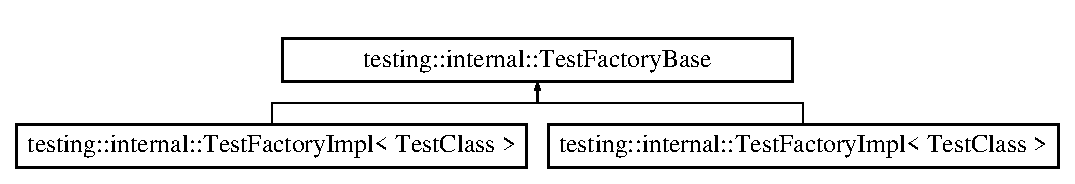
\includegraphics[height=2.000000cm]{classtesting_1_1internal_1_1_test_factory_base}
\end{center}
\end{figure}
\subsection*{Public Member Functions}
\begin{DoxyCompactItemize}
\item 
\hypertarget{classtesting_1_1internal_1_1_test_factory_base_a07ac3ca0b196cdb092da0bb186b7c030}{}virtual \hyperlink{classtesting_1_1_test}{Test} $\ast$ {\bfseries Create\+Test} ()=0\label{classtesting_1_1internal_1_1_test_factory_base_a07ac3ca0b196cdb092da0bb186b7c030}

\item 
\hypertarget{classtesting_1_1internal_1_1_test_factory_base_a07ac3ca0b196cdb092da0bb186b7c030}{}virtual \hyperlink{classtesting_1_1_test}{Test} $\ast$ {\bfseries Create\+Test} ()=0\label{classtesting_1_1internal_1_1_test_factory_base_a07ac3ca0b196cdb092da0bb186b7c030}

\end{DoxyCompactItemize}


The documentation for this class was generated from the following file\+:\begin{DoxyCompactItemize}
\item 
deps/win32/debug/include/gtest/internal/gtest-\/internal.\+h\end{DoxyCompactItemize}

\hypertarget{classtesting_1_1internal_1_1_test_factory_impl}{}\section{testing\+:\+:internal\+:\+:Test\+Factory\+Impl$<$ Test\+Class $>$ Class Template Reference}
\label{classtesting_1_1internal_1_1_test_factory_impl}\index{testing\+::internal\+::\+Test\+Factory\+Impl$<$ Test\+Class $>$@{testing\+::internal\+::\+Test\+Factory\+Impl$<$ Test\+Class $>$}}
Inheritance diagram for testing\+:\+:internal\+:\+:Test\+Factory\+Impl$<$ Test\+Class $>$\+:\begin{figure}[H]
\begin{center}
\leavevmode
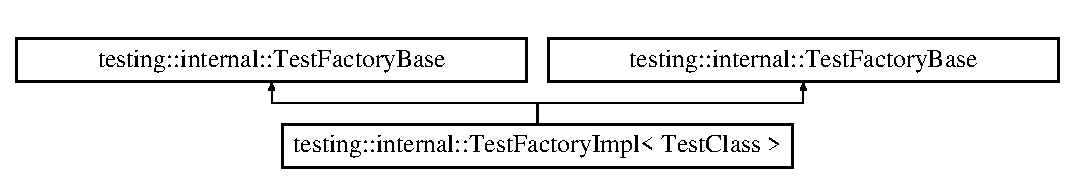
\includegraphics[height=2.000000cm]{classtesting_1_1internal_1_1_test_factory_impl}
\end{center}
\end{figure}
\subsection*{Public Member Functions}
\begin{DoxyCompactItemize}
\item 
\hypertarget{classtesting_1_1internal_1_1_test_factory_impl_a8860c89bdb06450a5d5e8137ebd9d775}{}virtual \hyperlink{classtesting_1_1_test}{Test} $\ast$ {\bfseries Create\+Test} ()\label{classtesting_1_1internal_1_1_test_factory_impl_a8860c89bdb06450a5d5e8137ebd9d775}

\item 
\hypertarget{classtesting_1_1internal_1_1_test_factory_impl_a8860c89bdb06450a5d5e8137ebd9d775}{}virtual \hyperlink{classtesting_1_1_test}{Test} $\ast$ {\bfseries Create\+Test} ()\label{classtesting_1_1internal_1_1_test_factory_impl_a8860c89bdb06450a5d5e8137ebd9d775}

\end{DoxyCompactItemize}


The documentation for this class was generated from the following file\+:\begin{DoxyCompactItemize}
\item 
deps/win32/debug/include/gtest/internal/gtest-\/internal.\+h\end{DoxyCompactItemize}

\hypertarget{classtesting_1_1_test_info}{}\section{testing\+:\+:Test\+Info Class Reference}
\label{classtesting_1_1_test_info}\index{testing\+::\+Test\+Info@{testing\+::\+Test\+Info}}
\subsection*{Public Member Functions}
\begin{DoxyCompactItemize}
\item 
\hypertarget{classtesting_1_1_test_info_a26d22556d04b94c9cd15e28d74fef91c}{}const char $\ast$ {\bfseries test\+\_\+case\+\_\+name} () const \label{classtesting_1_1_test_info_a26d22556d04b94c9cd15e28d74fef91c}

\item 
\hypertarget{classtesting_1_1_test_info_ab3d24cad310f0cde29a80b9a83949ff5}{}const char $\ast$ {\bfseries name} () const \label{classtesting_1_1_test_info_ab3d24cad310f0cde29a80b9a83949ff5}

\item 
\hypertarget{classtesting_1_1_test_info_af15d5c533a7237ffc183bc4c924dfcf4}{}const char $\ast$ {\bfseries type\+\_\+param} () const \label{classtesting_1_1_test_info_af15d5c533a7237ffc183bc4c924dfcf4}

\item 
\hypertarget{classtesting_1_1_test_info_a9671fbc0effcb32e98803888dc166a66}{}const char $\ast$ {\bfseries value\+\_\+param} () const \label{classtesting_1_1_test_info_a9671fbc0effcb32e98803888dc166a66}

\item 
\hypertarget{classtesting_1_1_test_info_a240c9fb051d7b0586ed380c6b4e729e4}{}bool {\bfseries should\+\_\+run} () const \label{classtesting_1_1_test_info_a240c9fb051d7b0586ed380c6b4e729e4}

\item 
\hypertarget{classtesting_1_1_test_info_a7ad90aeebb1d6fe3a43c6e3e3427e382}{}bool {\bfseries is\+\_\+reportable} () const \label{classtesting_1_1_test_info_a7ad90aeebb1d6fe3a43c6e3e3427e382}

\item 
\hypertarget{classtesting_1_1_test_info_addea8766df3b8abe4cc4103218a49a65}{}const \hyperlink{classtesting_1_1_test_result}{Test\+Result} $\ast$ {\bfseries result} () const \label{classtesting_1_1_test_info_addea8766df3b8abe4cc4103218a49a65}

\item 
\hypertarget{classtesting_1_1_test_info_a26d22556d04b94c9cd15e28d74fef91c}{}const char $\ast$ {\bfseries test\+\_\+case\+\_\+name} () const \label{classtesting_1_1_test_info_a26d22556d04b94c9cd15e28d74fef91c}

\item 
\hypertarget{classtesting_1_1_test_info_ab3d24cad310f0cde29a80b9a83949ff5}{}const char $\ast$ {\bfseries name} () const \label{classtesting_1_1_test_info_ab3d24cad310f0cde29a80b9a83949ff5}

\item 
\hypertarget{classtesting_1_1_test_info_af15d5c533a7237ffc183bc4c924dfcf4}{}const char $\ast$ {\bfseries type\+\_\+param} () const \label{classtesting_1_1_test_info_af15d5c533a7237ffc183bc4c924dfcf4}

\item 
\hypertarget{classtesting_1_1_test_info_a9671fbc0effcb32e98803888dc166a66}{}const char $\ast$ {\bfseries value\+\_\+param} () const \label{classtesting_1_1_test_info_a9671fbc0effcb32e98803888dc166a66}

\item 
\hypertarget{classtesting_1_1_test_info_a240c9fb051d7b0586ed380c6b4e729e4}{}bool {\bfseries should\+\_\+run} () const \label{classtesting_1_1_test_info_a240c9fb051d7b0586ed380c6b4e729e4}

\item 
\hypertarget{classtesting_1_1_test_info_a7ad90aeebb1d6fe3a43c6e3e3427e382}{}bool {\bfseries is\+\_\+reportable} () const \label{classtesting_1_1_test_info_a7ad90aeebb1d6fe3a43c6e3e3427e382}

\item 
\hypertarget{classtesting_1_1_test_info_addea8766df3b8abe4cc4103218a49a65}{}const \hyperlink{classtesting_1_1_test_result}{Test\+Result} $\ast$ {\bfseries result} () const \label{classtesting_1_1_test_info_addea8766df3b8abe4cc4103218a49a65}

\end{DoxyCompactItemize}
\subsection*{Friends}
\begin{DoxyCompactItemize}
\item 
\hypertarget{classtesting_1_1_test_info_ab085d1bf4cff8b1045750706b11f8662}{}class {\bfseries Test}\label{classtesting_1_1_test_info_ab085d1bf4cff8b1045750706b11f8662}

\item 
\hypertarget{classtesting_1_1_test_info_a61fe0349d692eb6d4f5b94e35049b2e9}{}class {\bfseries Test\+Case}\label{classtesting_1_1_test_info_a61fe0349d692eb6d4f5b94e35049b2e9}

\item 
\hypertarget{classtesting_1_1_test_info_aa684cc13a8f91b00c0c9ce41ec7474eb}{}class {\bfseries internal\+::\+Unit\+Test\+Impl}\label{classtesting_1_1_test_info_aa684cc13a8f91b00c0c9ce41ec7474eb}

\item 
\hypertarget{classtesting_1_1_test_info_a2021083660b7387a257fb6c6242fee73}{}class {\bfseries internal\+::\+Streaming\+Listener\+Test}\label{classtesting_1_1_test_info_a2021083660b7387a257fb6c6242fee73}

\item 
\hypertarget{classtesting_1_1_test_info_a3e27fa5e97044d379b1e3b2a753f56f8}{}\hyperlink{classtesting_1_1_test_info}{Test\+Info} $\ast$ {\bfseries internal\+::\+Make\+And\+Register\+Test\+Info} (const char $\ast$test\+\_\+case\+\_\+name, const char $\ast$name, const char $\ast$type\+\_\+param, const char $\ast$value\+\_\+param, internal\+::\+Type\+Id fixture\+\_\+class\+\_\+id, Test\+::\+Set\+Up\+Test\+Case\+Func set\+\_\+up\+\_\+tc, Test\+::\+Tear\+Down\+Test\+Case\+Func tear\+\_\+down\+\_\+tc, \hyperlink{classtesting_1_1internal_1_1_test_factory_base}{internal\+::\+Test\+Factory\+Base} $\ast$factory)\label{classtesting_1_1_test_info_a3e27fa5e97044d379b1e3b2a753f56f8}

\item 
\hypertarget{classtesting_1_1_test_info_a3e27fa5e97044d379b1e3b2a753f56f8}{}\hyperlink{classtesting_1_1_test_info}{Test\+Info} $\ast$ {\bfseries internal\+::\+Make\+And\+Register\+Test\+Info} (const char $\ast$test\+\_\+case\+\_\+name, const char $\ast$name, const char $\ast$type\+\_\+param, const char $\ast$value\+\_\+param, internal\+::\+Type\+Id fixture\+\_\+class\+\_\+id, Test\+::\+Set\+Up\+Test\+Case\+Func set\+\_\+up\+\_\+tc, Test\+::\+Tear\+Down\+Test\+Case\+Func tear\+\_\+down\+\_\+tc, \hyperlink{classtesting_1_1internal_1_1_test_factory_base}{internal\+::\+Test\+Factory\+Base} $\ast$factory)\label{classtesting_1_1_test_info_a3e27fa5e97044d379b1e3b2a753f56f8}

\end{DoxyCompactItemize}


The documentation for this class was generated from the following file\+:\begin{DoxyCompactItemize}
\item 
deps/win32/debug/include/gtest/gtest.\+h\end{DoxyCompactItemize}

\hypertarget{classtesting_1_1_test_part_result}{}\section{testing\+:\+:Test\+Part\+Result Class Reference}
\label{classtesting_1_1_test_part_result}\index{testing\+::\+Test\+Part\+Result@{testing\+::\+Test\+Part\+Result}}
\subsection*{Public Types}
\begin{DoxyCompactItemize}
\item 
\hypertarget{classtesting_1_1_test_part_result_a65ae656b33fdfdfffaf34858778a52d5}{}enum {\bfseries Type} \{ \\*
{\bfseries k\+Success}, 
{\bfseries k\+Non\+Fatal\+Failure}, 
{\bfseries k\+Fatal\+Failure}, 
{\bfseries k\+Success}, 
\\*
{\bfseries k\+Non\+Fatal\+Failure}, 
{\bfseries k\+Fatal\+Failure}
 \}\label{classtesting_1_1_test_part_result_a65ae656b33fdfdfffaf34858778a52d5}

\item 
\hypertarget{classtesting_1_1_test_part_result_a65ae656b33fdfdfffaf34858778a52d5}{}enum {\bfseries Type} \{ \\*
{\bfseries k\+Success}, 
{\bfseries k\+Non\+Fatal\+Failure}, 
{\bfseries k\+Fatal\+Failure}, 
{\bfseries k\+Success}, 
\\*
{\bfseries k\+Non\+Fatal\+Failure}, 
{\bfseries k\+Fatal\+Failure}
 \}\label{classtesting_1_1_test_part_result_a65ae656b33fdfdfffaf34858778a52d5}

\end{DoxyCompactItemize}
\subsection*{Public Member Functions}
\begin{DoxyCompactItemize}
\item 
\hypertarget{classtesting_1_1_test_part_result_a6409eb519c1cd514aab2426c8f40737f}{}{\bfseries Test\+Part\+Result} (Type a\+\_\+type, const char $\ast$a\+\_\+file\+\_\+name, int a\+\_\+line\+\_\+number, const char $\ast$a\+\_\+message)\label{classtesting_1_1_test_part_result_a6409eb519c1cd514aab2426c8f40737f}

\item 
\hypertarget{classtesting_1_1_test_part_result_ae852bf8693f066078c74c34345531940}{}Type {\bfseries type} () const \label{classtesting_1_1_test_part_result_ae852bf8693f066078c74c34345531940}

\item 
\hypertarget{classtesting_1_1_test_part_result_a5d8742dc28ddb880cd2391edb9fc2c9b}{}const char $\ast$ {\bfseries file\+\_\+name} () const \label{classtesting_1_1_test_part_result_a5d8742dc28ddb880cd2391edb9fc2c9b}

\item 
\hypertarget{classtesting_1_1_test_part_result_a174900cf4403d23784af34f50e7b0a46}{}int {\bfseries line\+\_\+number} () const \label{classtesting_1_1_test_part_result_a174900cf4403d23784af34f50e7b0a46}

\item 
\hypertarget{classtesting_1_1_test_part_result_af0d4f960b453ce087c581fe13817b2a3}{}const char $\ast$ {\bfseries summary} () const \label{classtesting_1_1_test_part_result_af0d4f960b453ce087c581fe13817b2a3}

\item 
\hypertarget{classtesting_1_1_test_part_result_aae73962246be4d200e2c1d04246a708a}{}const char $\ast$ {\bfseries message} () const \label{classtesting_1_1_test_part_result_aae73962246be4d200e2c1d04246a708a}

\item 
\hypertarget{classtesting_1_1_test_part_result_a901bd62d9fbe7f39826a9d02ab2bdaec}{}bool {\bfseries passed} () const \label{classtesting_1_1_test_part_result_a901bd62d9fbe7f39826a9d02ab2bdaec}

\item 
\hypertarget{classtesting_1_1_test_part_result_aaf835515fb53eb1aa01c1798b05e61f6}{}bool {\bfseries failed} () const \label{classtesting_1_1_test_part_result_aaf835515fb53eb1aa01c1798b05e61f6}

\item 
\hypertarget{classtesting_1_1_test_part_result_a7bb08c87fbc1664f9fcca1504339ed29}{}bool {\bfseries nonfatally\+\_\+failed} () const \label{classtesting_1_1_test_part_result_a7bb08c87fbc1664f9fcca1504339ed29}

\item 
\hypertarget{classtesting_1_1_test_part_result_a34d31718b5fc6c06f73d03e8dbb1aa9e}{}bool {\bfseries fatally\+\_\+failed} () const \label{classtesting_1_1_test_part_result_a34d31718b5fc6c06f73d03e8dbb1aa9e}

\item 
\hypertarget{classtesting_1_1_test_part_result_a6409eb519c1cd514aab2426c8f40737f}{}{\bfseries Test\+Part\+Result} (Type a\+\_\+type, const char $\ast$a\+\_\+file\+\_\+name, int a\+\_\+line\+\_\+number, const char $\ast$a\+\_\+message)\label{classtesting_1_1_test_part_result_a6409eb519c1cd514aab2426c8f40737f}

\item 
\hypertarget{classtesting_1_1_test_part_result_ae852bf8693f066078c74c34345531940}{}Type {\bfseries type} () const \label{classtesting_1_1_test_part_result_ae852bf8693f066078c74c34345531940}

\item 
\hypertarget{classtesting_1_1_test_part_result_a5d8742dc28ddb880cd2391edb9fc2c9b}{}const char $\ast$ {\bfseries file\+\_\+name} () const \label{classtesting_1_1_test_part_result_a5d8742dc28ddb880cd2391edb9fc2c9b}

\item 
\hypertarget{classtesting_1_1_test_part_result_a174900cf4403d23784af34f50e7b0a46}{}int {\bfseries line\+\_\+number} () const \label{classtesting_1_1_test_part_result_a174900cf4403d23784af34f50e7b0a46}

\item 
\hypertarget{classtesting_1_1_test_part_result_af0d4f960b453ce087c581fe13817b2a3}{}const char $\ast$ {\bfseries summary} () const \label{classtesting_1_1_test_part_result_af0d4f960b453ce087c581fe13817b2a3}

\item 
\hypertarget{classtesting_1_1_test_part_result_aae73962246be4d200e2c1d04246a708a}{}const char $\ast$ {\bfseries message} () const \label{classtesting_1_1_test_part_result_aae73962246be4d200e2c1d04246a708a}

\item 
\hypertarget{classtesting_1_1_test_part_result_a901bd62d9fbe7f39826a9d02ab2bdaec}{}bool {\bfseries passed} () const \label{classtesting_1_1_test_part_result_a901bd62d9fbe7f39826a9d02ab2bdaec}

\item 
\hypertarget{classtesting_1_1_test_part_result_aaf835515fb53eb1aa01c1798b05e61f6}{}bool {\bfseries failed} () const \label{classtesting_1_1_test_part_result_aaf835515fb53eb1aa01c1798b05e61f6}

\item 
\hypertarget{classtesting_1_1_test_part_result_a7bb08c87fbc1664f9fcca1504339ed29}{}bool {\bfseries nonfatally\+\_\+failed} () const \label{classtesting_1_1_test_part_result_a7bb08c87fbc1664f9fcca1504339ed29}

\item 
\hypertarget{classtesting_1_1_test_part_result_a34d31718b5fc6c06f73d03e8dbb1aa9e}{}bool {\bfseries fatally\+\_\+failed} () const \label{classtesting_1_1_test_part_result_a34d31718b5fc6c06f73d03e8dbb1aa9e}

\end{DoxyCompactItemize}


The documentation for this class was generated from the following file\+:\begin{DoxyCompactItemize}
\item 
deps/win32/debug/include/gtest/gtest-\/test-\/part.\+h\end{DoxyCompactItemize}

\hypertarget{classtesting_1_1_test_part_result_array}{}\section{testing\+:\+:Test\+Part\+Result\+Array Class Reference}
\label{classtesting_1_1_test_part_result_array}\index{testing\+::\+Test\+Part\+Result\+Array@{testing\+::\+Test\+Part\+Result\+Array}}
\subsection*{Public Member Functions}
\begin{DoxyCompactItemize}
\item 
\hypertarget{classtesting_1_1_test_part_result_array_a01844bd505b18a666324617a1b459558}{}void {\bfseries Append} (const \hyperlink{classtesting_1_1_test_part_result}{Test\+Part\+Result} \&result)\label{classtesting_1_1_test_part_result_array_a01844bd505b18a666324617a1b459558}

\item 
\hypertarget{classtesting_1_1_test_part_result_array_a2b3dbf4012f204d916ce4a374bc03da4}{}const \hyperlink{classtesting_1_1_test_part_result}{Test\+Part\+Result} \& {\bfseries Get\+Test\+Part\+Result} (int index) const \label{classtesting_1_1_test_part_result_array_a2b3dbf4012f204d916ce4a374bc03da4}

\item 
\hypertarget{classtesting_1_1_test_part_result_array_acd805ad4edda06d983456b2a30760dce}{}int {\bfseries size} () const \label{classtesting_1_1_test_part_result_array_acd805ad4edda06d983456b2a30760dce}

\item 
\hypertarget{classtesting_1_1_test_part_result_array_a01844bd505b18a666324617a1b459558}{}void {\bfseries Append} (const \hyperlink{classtesting_1_1_test_part_result}{Test\+Part\+Result} \&result)\label{classtesting_1_1_test_part_result_array_a01844bd505b18a666324617a1b459558}

\item 
\hypertarget{classtesting_1_1_test_part_result_array_a2b3dbf4012f204d916ce4a374bc03da4}{}const \hyperlink{classtesting_1_1_test_part_result}{Test\+Part\+Result} \& {\bfseries Get\+Test\+Part\+Result} (int index) const \label{classtesting_1_1_test_part_result_array_a2b3dbf4012f204d916ce4a374bc03da4}

\item 
\hypertarget{classtesting_1_1_test_part_result_array_acd805ad4edda06d983456b2a30760dce}{}int {\bfseries size} () const \label{classtesting_1_1_test_part_result_array_acd805ad4edda06d983456b2a30760dce}

\end{DoxyCompactItemize}


The documentation for this class was generated from the following file\+:\begin{DoxyCompactItemize}
\item 
deps/win32/debug/include/gtest/gtest-\/test-\/part.\+h\end{DoxyCompactItemize}

\hypertarget{classtesting_1_1_test_part_result_reporter_interface}{}\section{testing\+:\+:Test\+Part\+Result\+Reporter\+Interface Class Reference}
\label{classtesting_1_1_test_part_result_reporter_interface}\index{testing\+::\+Test\+Part\+Result\+Reporter\+Interface@{testing\+::\+Test\+Part\+Result\+Reporter\+Interface}}
Inheritance diagram for testing\+:\+:Test\+Part\+Result\+Reporter\+Interface\+:\begin{figure}[H]
\begin{center}
\leavevmode
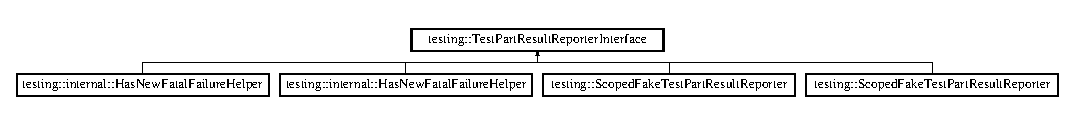
\includegraphics[height=1.064639cm]{classtesting_1_1_test_part_result_reporter_interface}
\end{center}
\end{figure}
\subsection*{Public Member Functions}
\begin{DoxyCompactItemize}
\item 
\hypertarget{classtesting_1_1_test_part_result_reporter_interface_aa2f920e7a5a0a6d0faf19e3727928c22}{}virtual void {\bfseries Report\+Test\+Part\+Result} (const \hyperlink{classtesting_1_1_test_part_result}{Test\+Part\+Result} \&result)=0\label{classtesting_1_1_test_part_result_reporter_interface_aa2f920e7a5a0a6d0faf19e3727928c22}

\item 
\hypertarget{classtesting_1_1_test_part_result_reporter_interface_aa2f920e7a5a0a6d0faf19e3727928c22}{}virtual void {\bfseries Report\+Test\+Part\+Result} (const \hyperlink{classtesting_1_1_test_part_result}{Test\+Part\+Result} \&result)=0\label{classtesting_1_1_test_part_result_reporter_interface_aa2f920e7a5a0a6d0faf19e3727928c22}

\end{DoxyCompactItemize}


The documentation for this class was generated from the following file\+:\begin{DoxyCompactItemize}
\item 
deps/win32/debug/include/gtest/gtest-\/test-\/part.\+h\end{DoxyCompactItemize}

\hypertarget{classtesting_1_1_test_property}{}\section{testing\+:\+:Test\+Property Class Reference}
\label{classtesting_1_1_test_property}\index{testing\+::\+Test\+Property@{testing\+::\+Test\+Property}}
\subsection*{Public Member Functions}
\begin{DoxyCompactItemize}
\item 
\hypertarget{classtesting_1_1_test_property_a25a0ccf1c75a92af46a48d3c2a873e6d}{}{\bfseries Test\+Property} (const std\+::string \&a\+\_\+key, const std\+::string \&a\+\_\+value)\label{classtesting_1_1_test_property_a25a0ccf1c75a92af46a48d3c2a873e6d}

\item 
\hypertarget{classtesting_1_1_test_property_a2c569d47685b89aa64e737fb11df3aba}{}const char $\ast$ {\bfseries key} () const \label{classtesting_1_1_test_property_a2c569d47685b89aa64e737fb11df3aba}

\item 
\hypertarget{classtesting_1_1_test_property_ad46323c18491f365d72d8a4288f54bd6}{}const char $\ast$ {\bfseries value} () const \label{classtesting_1_1_test_property_ad46323c18491f365d72d8a4288f54bd6}

\item 
\hypertarget{classtesting_1_1_test_property_a377245335d9f614cd06d1650e3358e1d}{}void {\bfseries Set\+Value} (const std\+::string \&new\+\_\+value)\label{classtesting_1_1_test_property_a377245335d9f614cd06d1650e3358e1d}

\item 
\hypertarget{classtesting_1_1_test_property_a25a0ccf1c75a92af46a48d3c2a873e6d}{}{\bfseries Test\+Property} (const std\+::string \&a\+\_\+key, const std\+::string \&a\+\_\+value)\label{classtesting_1_1_test_property_a25a0ccf1c75a92af46a48d3c2a873e6d}

\item 
\hypertarget{classtesting_1_1_test_property_a2c569d47685b89aa64e737fb11df3aba}{}const char $\ast$ {\bfseries key} () const \label{classtesting_1_1_test_property_a2c569d47685b89aa64e737fb11df3aba}

\item 
\hypertarget{classtesting_1_1_test_property_ad46323c18491f365d72d8a4288f54bd6}{}const char $\ast$ {\bfseries value} () const \label{classtesting_1_1_test_property_ad46323c18491f365d72d8a4288f54bd6}

\item 
\hypertarget{classtesting_1_1_test_property_a377245335d9f614cd06d1650e3358e1d}{}void {\bfseries Set\+Value} (const std\+::string \&new\+\_\+value)\label{classtesting_1_1_test_property_a377245335d9f614cd06d1650e3358e1d}

\end{DoxyCompactItemize}


The documentation for this class was generated from the following file\+:\begin{DoxyCompactItemize}
\item 
deps/win32/debug/include/gtest/gtest.\+h\end{DoxyCompactItemize}

\hypertarget{classtesting_1_1_test_result}{}\section{testing\+:\+:Test\+Result Class Reference}
\label{classtesting_1_1_test_result}\index{testing\+::\+Test\+Result@{testing\+::\+Test\+Result}}
\subsection*{Public Member Functions}
\begin{DoxyCompactItemize}
\item 
\hypertarget{classtesting_1_1_test_result_ae6a378ec743edfbed55890c955d0adc8}{}int {\bfseries total\+\_\+part\+\_\+count} () const \label{classtesting_1_1_test_result_ae6a378ec743edfbed55890c955d0adc8}

\item 
\hypertarget{classtesting_1_1_test_result_a5075f9d595d51c7cc2f5c0921e622831}{}int {\bfseries test\+\_\+property\+\_\+count} () const \label{classtesting_1_1_test_result_a5075f9d595d51c7cc2f5c0921e622831}

\item 
\hypertarget{classtesting_1_1_test_result_aa46a04342f02ec297357f47288da3ef3}{}bool {\bfseries Passed} () const \label{classtesting_1_1_test_result_aa46a04342f02ec297357f47288da3ef3}

\item 
\hypertarget{classtesting_1_1_test_result_abb5d051bf958071c14020132a4d6cc07}{}bool {\bfseries Failed} () const \label{classtesting_1_1_test_result_abb5d051bf958071c14020132a4d6cc07}

\item 
\hypertarget{classtesting_1_1_test_result_ace61ce992083a9124f9ff0e99a2041cc}{}bool {\bfseries Has\+Fatal\+Failure} () const \label{classtesting_1_1_test_result_ace61ce992083a9124f9ff0e99a2041cc}

\item 
\hypertarget{classtesting_1_1_test_result_a34e6901b9772f51ce4f17a5517c26607}{}bool {\bfseries Has\+Nonfatal\+Failure} () const \label{classtesting_1_1_test_result_a34e6901b9772f51ce4f17a5517c26607}

\item 
\hypertarget{classtesting_1_1_test_result_a582f6383265d0619df812b75499d0616}{}Time\+In\+Millis {\bfseries elapsed\+\_\+time} () const \label{classtesting_1_1_test_result_a582f6383265d0619df812b75499d0616}

\item 
\hypertarget{classtesting_1_1_test_result_a5ea65e4a7c4fc9c9dc9578223a599a7c}{}const \hyperlink{classtesting_1_1_test_part_result}{Test\+Part\+Result} \& {\bfseries Get\+Test\+Part\+Result} (int i) const \label{classtesting_1_1_test_result_a5ea65e4a7c4fc9c9dc9578223a599a7c}

\item 
\hypertarget{classtesting_1_1_test_result_a89a4f580a5d969b36e016cd309b235bd}{}const \hyperlink{classtesting_1_1_test_property}{Test\+Property} \& {\bfseries Get\+Test\+Property} (int i) const \label{classtesting_1_1_test_result_a89a4f580a5d969b36e016cd309b235bd}

\item 
\hypertarget{classtesting_1_1_test_result_ae6a378ec743edfbed55890c955d0adc8}{}int {\bfseries total\+\_\+part\+\_\+count} () const \label{classtesting_1_1_test_result_ae6a378ec743edfbed55890c955d0adc8}

\item 
\hypertarget{classtesting_1_1_test_result_a5075f9d595d51c7cc2f5c0921e622831}{}int {\bfseries test\+\_\+property\+\_\+count} () const \label{classtesting_1_1_test_result_a5075f9d595d51c7cc2f5c0921e622831}

\item 
\hypertarget{classtesting_1_1_test_result_aa46a04342f02ec297357f47288da3ef3}{}bool {\bfseries Passed} () const \label{classtesting_1_1_test_result_aa46a04342f02ec297357f47288da3ef3}

\item 
\hypertarget{classtesting_1_1_test_result_abb5d051bf958071c14020132a4d6cc07}{}bool {\bfseries Failed} () const \label{classtesting_1_1_test_result_abb5d051bf958071c14020132a4d6cc07}

\item 
\hypertarget{classtesting_1_1_test_result_ace61ce992083a9124f9ff0e99a2041cc}{}bool {\bfseries Has\+Fatal\+Failure} () const \label{classtesting_1_1_test_result_ace61ce992083a9124f9ff0e99a2041cc}

\item 
\hypertarget{classtesting_1_1_test_result_a34e6901b9772f51ce4f17a5517c26607}{}bool {\bfseries Has\+Nonfatal\+Failure} () const \label{classtesting_1_1_test_result_a34e6901b9772f51ce4f17a5517c26607}

\item 
\hypertarget{classtesting_1_1_test_result_a582f6383265d0619df812b75499d0616}{}Time\+In\+Millis {\bfseries elapsed\+\_\+time} () const \label{classtesting_1_1_test_result_a582f6383265d0619df812b75499d0616}

\item 
\hypertarget{classtesting_1_1_test_result_a5ea65e4a7c4fc9c9dc9578223a599a7c}{}const \hyperlink{classtesting_1_1_test_part_result}{Test\+Part\+Result} \& {\bfseries Get\+Test\+Part\+Result} (int i) const \label{classtesting_1_1_test_result_a5ea65e4a7c4fc9c9dc9578223a599a7c}

\item 
\hypertarget{classtesting_1_1_test_result_a89a4f580a5d969b36e016cd309b235bd}{}const \hyperlink{classtesting_1_1_test_property}{Test\+Property} \& {\bfseries Get\+Test\+Property} (int i) const \label{classtesting_1_1_test_result_a89a4f580a5d969b36e016cd309b235bd}

\end{DoxyCompactItemize}
\subsection*{Friends}
\begin{DoxyCompactItemize}
\item 
\hypertarget{classtesting_1_1_test_result_aed3c96e2bd5a46339c1cbe49a4a233ee}{}class {\bfseries Test\+Info}\label{classtesting_1_1_test_result_aed3c96e2bd5a46339c1cbe49a4a233ee}

\item 
\hypertarget{classtesting_1_1_test_result_a61fe0349d692eb6d4f5b94e35049b2e9}{}class {\bfseries Test\+Case}\label{classtesting_1_1_test_result_a61fe0349d692eb6d4f5b94e35049b2e9}

\item 
\hypertarget{classtesting_1_1_test_result_aaeb07ea6ba11473f5b2ff2067a1d734a}{}class {\bfseries Unit\+Test}\label{classtesting_1_1_test_result_aaeb07ea6ba11473f5b2ff2067a1d734a}

\item 
\hypertarget{classtesting_1_1_test_result_ac731f0389a3fc3cae64a80a5e53acc2a}{}class {\bfseries internal\+::\+Default\+Global\+Test\+Part\+Result\+Reporter}\label{classtesting_1_1_test_result_ac731f0389a3fc3cae64a80a5e53acc2a}

\item 
\hypertarget{classtesting_1_1_test_result_a6a009268369159ee3ff3d162e5c9f0b4}{}class {\bfseries internal\+::\+Exec\+Death\+Test}\label{classtesting_1_1_test_result_a6a009268369159ee3ff3d162e5c9f0b4}

\item 
\hypertarget{classtesting_1_1_test_result_a9409280e3d708ddb050e1b9922b91522}{}class {\bfseries internal\+::\+Test\+Result\+Accessor}\label{classtesting_1_1_test_result_a9409280e3d708ddb050e1b9922b91522}

\item 
\hypertarget{classtesting_1_1_test_result_aa684cc13a8f91b00c0c9ce41ec7474eb}{}class {\bfseries internal\+::\+Unit\+Test\+Impl}\label{classtesting_1_1_test_result_aa684cc13a8f91b00c0c9ce41ec7474eb}

\item 
\hypertarget{classtesting_1_1_test_result_ab7ea7e66d98b6380f6216e44ce744390}{}class {\bfseries internal\+::\+Windows\+Death\+Test}\label{classtesting_1_1_test_result_ab7ea7e66d98b6380f6216e44ce744390}

\end{DoxyCompactItemize}


The documentation for this class was generated from the following file\+:\begin{DoxyCompactItemize}
\item 
deps/win32/debug/include/gtest/gtest.\+h\end{DoxyCompactItemize}

\hypertarget{classtesting_1_1internal_1_1_thread_local}{}\section{testing\+:\+:internal\+:\+:Thread\+Local$<$ T $>$ Class Template Reference}
\label{classtesting_1_1internal_1_1_thread_local}\index{testing\+::internal\+::\+Thread\+Local$<$ T $>$@{testing\+::internal\+::\+Thread\+Local$<$ T $>$}}
\subsection*{Public Member Functions}
\begin{DoxyCompactItemize}
\item 
\hypertarget{classtesting_1_1internal_1_1_thread_local_a85610bdfdbc93a4c56215e0aad7da870}{}{\bfseries Thread\+Local} (const T \&value)\label{classtesting_1_1internal_1_1_thread_local_a85610bdfdbc93a4c56215e0aad7da870}

\item 
\hypertarget{classtesting_1_1internal_1_1_thread_local_a882f57fed4b074de83693c0c0fe62858}{}T $\ast$ {\bfseries pointer} ()\label{classtesting_1_1internal_1_1_thread_local_a882f57fed4b074de83693c0c0fe62858}

\item 
\hypertarget{classtesting_1_1internal_1_1_thread_local_af4b33c12fd2da7d43d8654feccca77f7}{}const T $\ast$ {\bfseries pointer} () const \label{classtesting_1_1internal_1_1_thread_local_af4b33c12fd2da7d43d8654feccca77f7}

\item 
\hypertarget{classtesting_1_1internal_1_1_thread_local_a9cfa47ae6e9e8c19fe8782e2e9c1b13e}{}const T \& {\bfseries get} () const \label{classtesting_1_1internal_1_1_thread_local_a9cfa47ae6e9e8c19fe8782e2e9c1b13e}

\item 
\hypertarget{classtesting_1_1internal_1_1_thread_local_ab5ebc7ba07426cef7167afa2a7707eb4}{}void {\bfseries set} (const T \&value)\label{classtesting_1_1internal_1_1_thread_local_ab5ebc7ba07426cef7167afa2a7707eb4}

\item 
\hypertarget{classtesting_1_1internal_1_1_thread_local_a85610bdfdbc93a4c56215e0aad7da870}{}{\bfseries Thread\+Local} (const T \&value)\label{classtesting_1_1internal_1_1_thread_local_a85610bdfdbc93a4c56215e0aad7da870}

\item 
\hypertarget{classtesting_1_1internal_1_1_thread_local_a882f57fed4b074de83693c0c0fe62858}{}T $\ast$ {\bfseries pointer} ()\label{classtesting_1_1internal_1_1_thread_local_a882f57fed4b074de83693c0c0fe62858}

\item 
\hypertarget{classtesting_1_1internal_1_1_thread_local_af4b33c12fd2da7d43d8654feccca77f7}{}const T $\ast$ {\bfseries pointer} () const \label{classtesting_1_1internal_1_1_thread_local_af4b33c12fd2da7d43d8654feccca77f7}

\item 
\hypertarget{classtesting_1_1internal_1_1_thread_local_a9cfa47ae6e9e8c19fe8782e2e9c1b13e}{}const T \& {\bfseries get} () const \label{classtesting_1_1internal_1_1_thread_local_a9cfa47ae6e9e8c19fe8782e2e9c1b13e}

\item 
\hypertarget{classtesting_1_1internal_1_1_thread_local_ab5ebc7ba07426cef7167afa2a7707eb4}{}void {\bfseries set} (const T \&value)\label{classtesting_1_1internal_1_1_thread_local_ab5ebc7ba07426cef7167afa2a7707eb4}

\end{DoxyCompactItemize}


The documentation for this class was generated from the following file\+:\begin{DoxyCompactItemize}
\item 
deps/win32/debug/include/gtest/internal/gtest-\/port.\+h\end{DoxyCompactItemize}

\hypertarget{classstd_1_1tr1_1_1tuple}{}\section{std\+:\+:tr1\+:\+:tuple$<$$>$ Class Template Reference}
\label{classstd_1_1tr1_1_1tuple}\index{std\+::tr1\+::tuple$<$$>$@{std\+::tr1\+::tuple$<$$>$}}
\subsection*{Public Member Functions}
\begin{DoxyCompactItemize}
\item 
\hypertarget{classstd_1_1tr1_1_1tuple_a349b7948d183b7f05c1a5fd6aa4eaeb8}{}{\bfseries tuple} (G\+T\+E\+S\+T\+\_\+\+B\+Y\+\_\+\+R\+E\+F\+\_\+(T0) f0, G\+T\+E\+S\+T\+\_\+\+B\+Y\+\_\+\+R\+E\+F\+\_\+(T1) f1, G\+T\+E\+S\+T\+\_\+\+B\+Y\+\_\+\+R\+E\+F\+\_\+(T2) f2, G\+T\+E\+S\+T\+\_\+\+B\+Y\+\_\+\+R\+E\+F\+\_\+(T3) f3, G\+T\+E\+S\+T\+\_\+\+B\+Y\+\_\+\+R\+E\+F\+\_\+(T4) f4, G\+T\+E\+S\+T\+\_\+\+B\+Y\+\_\+\+R\+E\+F\+\_\+(T5) f5, G\+T\+E\+S\+T\+\_\+\+B\+Y\+\_\+\+R\+E\+F\+\_\+(T6) f6, G\+T\+E\+S\+T\+\_\+\+B\+Y\+\_\+\+R\+E\+F\+\_\+(T7) f7, G\+T\+E\+S\+T\+\_\+\+B\+Y\+\_\+\+R\+E\+F\+\_\+(T8) f8, G\+T\+E\+S\+T\+\_\+\+B\+Y\+\_\+\+R\+E\+F\+\_\+(T9) f9)\label{classstd_1_1tr1_1_1tuple_a349b7948d183b7f05c1a5fd6aa4eaeb8}

\item 
\hypertarget{classstd_1_1tr1_1_1tuple_ade1807f6e6b36daa6387c3b00dbd3be6}{}{\bfseries tuple} (const \hyperlink{classstd_1_1tr1_1_1tuple}{tuple} \&t)\label{classstd_1_1tr1_1_1tuple_ade1807f6e6b36daa6387c3b00dbd3be6}

\item 
\hypertarget{classstd_1_1tr1_1_1tuple_a7ff289d5c5a605e4a4f8fb56913f7370}{}{\footnotesize template$<$G\+T\+E\+S\+T\+\_\+10\+\_\+\+T\+Y\+P\+E\+N\+A\+M\+E\+S\+\_\+(\+U) $>$ }\\{\bfseries tuple} (const G\+T\+E\+S\+T\+\_\+10\+\_\+\+T\+U\+P\+L\+E\+\_\+(U)\&t)\label{classstd_1_1tr1_1_1tuple_a7ff289d5c5a605e4a4f8fb56913f7370}

\item 
\hypertarget{classstd_1_1tr1_1_1tuple_ae52bd211e87c30ea7243246fa06bf038}{}\hyperlink{classstd_1_1tr1_1_1tuple}{tuple} \& {\bfseries operator=} (const \hyperlink{classstd_1_1tr1_1_1tuple}{tuple} \&t)\label{classstd_1_1tr1_1_1tuple_ae52bd211e87c30ea7243246fa06bf038}

\item 
\hypertarget{classstd_1_1tr1_1_1tuple_a9ed59ab84e2ff750d0a188c3d9dac819}{}{\footnotesize template$<$G\+T\+E\+S\+T\+\_\+10\+\_\+\+T\+Y\+P\+E\+N\+A\+M\+E\+S\+\_\+(\+U) $>$ }\\\hyperlink{classstd_1_1tr1_1_1tuple}{tuple} \& {\bfseries operator=} (const G\+T\+E\+S\+T\+\_\+10\+\_\+\+T\+U\+P\+L\+E\+\_\+(U)\&t)\label{classstd_1_1tr1_1_1tuple_a9ed59ab84e2ff750d0a188c3d9dac819}

\item 
\hypertarget{classstd_1_1tr1_1_1tuple_a3d06fb121d18b6e1c10d14f9e966618d}{}{\footnotesize template$<$G\+T\+E\+S\+T\+\_\+10\+\_\+\+T\+Y\+P\+E\+N\+A\+M\+E\+S\+\_\+(\+U) $>$ }\\G\+T\+E\+S\+T\+\_\+\+D\+E\+C\+L\+A\+R\+E\+\_\+\+T\+U\+P\+L\+E\+\_\+\+A\+S\+\_\+\+F\+R\+I\+E\+N\+D\+\_\+ \hyperlink{classstd_1_1tr1_1_1tuple}{tuple} \& {\bfseries Copy\+From} (const G\+T\+E\+S\+T\+\_\+10\+\_\+\+T\+U\+P\+L\+E\+\_\+(U)\&t)\label{classstd_1_1tr1_1_1tuple_a3d06fb121d18b6e1c10d14f9e966618d}

\item 
\hypertarget{classstd_1_1tr1_1_1tuple_a349b7948d183b7f05c1a5fd6aa4eaeb8}{}{\bfseries tuple} (G\+T\+E\+S\+T\+\_\+\+B\+Y\+\_\+\+R\+E\+F\+\_\+(T0) f0, G\+T\+E\+S\+T\+\_\+\+B\+Y\+\_\+\+R\+E\+F\+\_\+(T1) f1, G\+T\+E\+S\+T\+\_\+\+B\+Y\+\_\+\+R\+E\+F\+\_\+(T2) f2, G\+T\+E\+S\+T\+\_\+\+B\+Y\+\_\+\+R\+E\+F\+\_\+(T3) f3, G\+T\+E\+S\+T\+\_\+\+B\+Y\+\_\+\+R\+E\+F\+\_\+(T4) f4, G\+T\+E\+S\+T\+\_\+\+B\+Y\+\_\+\+R\+E\+F\+\_\+(T5) f5, G\+T\+E\+S\+T\+\_\+\+B\+Y\+\_\+\+R\+E\+F\+\_\+(T6) f6, G\+T\+E\+S\+T\+\_\+\+B\+Y\+\_\+\+R\+E\+F\+\_\+(T7) f7, G\+T\+E\+S\+T\+\_\+\+B\+Y\+\_\+\+R\+E\+F\+\_\+(T8) f8, G\+T\+E\+S\+T\+\_\+\+B\+Y\+\_\+\+R\+E\+F\+\_\+(T9) f9)\label{classstd_1_1tr1_1_1tuple_a349b7948d183b7f05c1a5fd6aa4eaeb8}

\item 
\hypertarget{classstd_1_1tr1_1_1tuple_ade1807f6e6b36daa6387c3b00dbd3be6}{}{\bfseries tuple} (const \hyperlink{classstd_1_1tr1_1_1tuple}{tuple} \&t)\label{classstd_1_1tr1_1_1tuple_ade1807f6e6b36daa6387c3b00dbd3be6}

\item 
\hypertarget{classstd_1_1tr1_1_1tuple_a7ff289d5c5a605e4a4f8fb56913f7370}{}{\footnotesize template$<$G\+T\+E\+S\+T\+\_\+10\+\_\+\+T\+Y\+P\+E\+N\+A\+M\+E\+S\+\_\+(\+U) $>$ }\\{\bfseries tuple} (const G\+T\+E\+S\+T\+\_\+10\+\_\+\+T\+U\+P\+L\+E\+\_\+(U)\&t)\label{classstd_1_1tr1_1_1tuple_a7ff289d5c5a605e4a4f8fb56913f7370}

\item 
\hypertarget{classstd_1_1tr1_1_1tuple_ae52bd211e87c30ea7243246fa06bf038}{}\hyperlink{classstd_1_1tr1_1_1tuple}{tuple} \& {\bfseries operator=} (const \hyperlink{classstd_1_1tr1_1_1tuple}{tuple} \&t)\label{classstd_1_1tr1_1_1tuple_ae52bd211e87c30ea7243246fa06bf038}

\item 
\hypertarget{classstd_1_1tr1_1_1tuple_a9ed59ab84e2ff750d0a188c3d9dac819}{}{\footnotesize template$<$G\+T\+E\+S\+T\+\_\+10\+\_\+\+T\+Y\+P\+E\+N\+A\+M\+E\+S\+\_\+(\+U) $>$ }\\\hyperlink{classstd_1_1tr1_1_1tuple}{tuple} \& {\bfseries operator=} (const G\+T\+E\+S\+T\+\_\+10\+\_\+\+T\+U\+P\+L\+E\+\_\+(U)\&t)\label{classstd_1_1tr1_1_1tuple_a9ed59ab84e2ff750d0a188c3d9dac819}

\item 
\hypertarget{classstd_1_1tr1_1_1tuple_a3d06fb121d18b6e1c10d14f9e966618d}{}{\footnotesize template$<$G\+T\+E\+S\+T\+\_\+10\+\_\+\+T\+Y\+P\+E\+N\+A\+M\+E\+S\+\_\+(\+U) $>$ }\\G\+T\+E\+S\+T\+\_\+\+D\+E\+C\+L\+A\+R\+E\+\_\+\+T\+U\+P\+L\+E\+\_\+\+A\+S\+\_\+\+F\+R\+I\+E\+N\+D\+\_\+ \hyperlink{classstd_1_1tr1_1_1tuple}{tuple} \& {\bfseries Copy\+From} (const G\+T\+E\+S\+T\+\_\+10\+\_\+\+T\+U\+P\+L\+E\+\_\+(U)\&t)\label{classstd_1_1tr1_1_1tuple_a3d06fb121d18b6e1c10d14f9e966618d}

\end{DoxyCompactItemize}
\subsection*{Public Attributes}
\begin{DoxyCompactItemize}
\item 
\hypertarget{classstd_1_1tr1_1_1tuple_a771b1d99e8800fb284acd04bca838cbb}{}T0 {\bfseries f0\+\_\+}\label{classstd_1_1tr1_1_1tuple_a771b1d99e8800fb284acd04bca838cbb}

\item 
\hypertarget{classstd_1_1tr1_1_1tuple_a7cccf899dedc626c51fa4f6921d0ac52}{}T1 {\bfseries f1\+\_\+}\label{classstd_1_1tr1_1_1tuple_a7cccf899dedc626c51fa4f6921d0ac52}

\item 
\hypertarget{classstd_1_1tr1_1_1tuple_aaec06c27366502dc332ef96878628f84}{}T2 {\bfseries f2\+\_\+}\label{classstd_1_1tr1_1_1tuple_aaec06c27366502dc332ef96878628f84}

\item 
\hypertarget{classstd_1_1tr1_1_1tuple_ad4d3673e0d5c07c392c02e335fe978ff}{}T3 {\bfseries f3\+\_\+}\label{classstd_1_1tr1_1_1tuple_ad4d3673e0d5c07c392c02e335fe978ff}

\item 
\hypertarget{classstd_1_1tr1_1_1tuple_ab662f1051c2302d065796383848db6c4}{}T4 {\bfseries f4\+\_\+}\label{classstd_1_1tr1_1_1tuple_ab662f1051c2302d065796383848db6c4}

\item 
\hypertarget{classstd_1_1tr1_1_1tuple_a32d8cd6f180c0a77d83733fc65423657}{}T5 {\bfseries f5\+\_\+}\label{classstd_1_1tr1_1_1tuple_a32d8cd6f180c0a77d83733fc65423657}

\item 
\hypertarget{classstd_1_1tr1_1_1tuple_a597beab3af3f95c84408491ab14632b0}{}T6 {\bfseries f6\+\_\+}\label{classstd_1_1tr1_1_1tuple_a597beab3af3f95c84408491ab14632b0}

\item 
\hypertarget{classstd_1_1tr1_1_1tuple_a7c28780e616d382833e844f62672c6bc}{}T7 {\bfseries f7\+\_\+}\label{classstd_1_1tr1_1_1tuple_a7c28780e616d382833e844f62672c6bc}

\item 
\hypertarget{classstd_1_1tr1_1_1tuple_ae859012c83943e54e035a4a32089ccb6}{}T8 {\bfseries f8\+\_\+}\label{classstd_1_1tr1_1_1tuple_ae859012c83943e54e035a4a32089ccb6}

\item 
\hypertarget{classstd_1_1tr1_1_1tuple_a336d5e582fd34e45ec88c78d473671dd}{}T9 {\bfseries f9\+\_\+}\label{classstd_1_1tr1_1_1tuple_a336d5e582fd34e45ec88c78d473671dd}

\end{DoxyCompactItemize}
\subsection*{Friends}
\begin{DoxyCompactItemize}
\item 
\hypertarget{classstd_1_1tr1_1_1tuple_aeeed38755abdaa78587dd1eac9ccc950}{}{\footnotesize template$<$int k$>$ }\\class {\bfseries gtest\+\_\+internal\+::\+Get}\label{classstd_1_1tr1_1_1tuple_aeeed38755abdaa78587dd1eac9ccc950}

\item 
\hypertarget{classstd_1_1tr1_1_1tuple_a266bb701b0bf866007d5865d36f87bd1}{}{\footnotesize template$<$int k$>$ }\\class {\bfseries gtest\+\_\+internal\+::\+Get}\label{classstd_1_1tr1_1_1tuple_a266bb701b0bf866007d5865d36f87bd1}

\end{DoxyCompactItemize}


The documentation for this class was generated from the following file\+:\begin{DoxyCompactItemize}
\item 
deps/win32/debug/include/gtest/internal/gtest-\/tuple.\+h\end{DoxyCompactItemize}

\hypertarget{classstd_1_1tr1_1_1tuple_3_4}{}\section{std\+:\+:tr1\+:\+:tuple$<$$>$ Class Template Reference}
\label{classstd_1_1tr1_1_1tuple_3_4}\index{std\+::tr1\+::tuple$<$$>$@{std\+::tr1\+::tuple$<$$>$}}
\subsection*{Public Member Functions}
\begin{DoxyCompactItemize}
\item 
\hypertarget{classstd_1_1tr1_1_1tuple_3_4_aa857599acb126134e29dc5e53fd9d1a7}{}{\bfseries tuple} (const \hyperlink{classstd_1_1tr1_1_1tuple}{tuple} \&)\label{classstd_1_1tr1_1_1tuple_3_4_aa857599acb126134e29dc5e53fd9d1a7}

\item 
\hypertarget{classstd_1_1tr1_1_1tuple_3_4_a93ddab6f662662fc49635608619150c8}{}\hyperlink{classstd_1_1tr1_1_1tuple}{tuple} \& {\bfseries operator=} (const \hyperlink{classstd_1_1tr1_1_1tuple}{tuple} \&)\label{classstd_1_1tr1_1_1tuple_3_4_a93ddab6f662662fc49635608619150c8}

\item 
\hypertarget{classstd_1_1tr1_1_1tuple_3_4_aa857599acb126134e29dc5e53fd9d1a7}{}{\bfseries tuple} (const \hyperlink{classstd_1_1tr1_1_1tuple}{tuple} \&)\label{classstd_1_1tr1_1_1tuple_3_4_aa857599acb126134e29dc5e53fd9d1a7}

\item 
\hypertarget{classstd_1_1tr1_1_1tuple_3_4_a93ddab6f662662fc49635608619150c8}{}\hyperlink{classstd_1_1tr1_1_1tuple}{tuple} \& {\bfseries operator=} (const \hyperlink{classstd_1_1tr1_1_1tuple}{tuple} \&)\label{classstd_1_1tr1_1_1tuple_3_4_a93ddab6f662662fc49635608619150c8}

\end{DoxyCompactItemize}


The documentation for this class was generated from the following file\+:\begin{DoxyCompactItemize}
\item 
deps/win32/debug/include/gtest/internal/gtest-\/tuple.\+h\end{DoxyCompactItemize}

\hypertarget{structstd_1_1tr1_1_1tuple__element}{}\section{std\+:\+:tr1\+:\+:tuple\+\_\+element$<$ k, Tuple $>$ Struct Template Reference}
\label{structstd_1_1tr1_1_1tuple__element}\index{std\+::tr1\+::tuple\+\_\+element$<$ k, Tuple $>$@{std\+::tr1\+::tuple\+\_\+element$<$ k, Tuple $>$}}


The documentation for this struct was generated from the following file\+:\begin{DoxyCompactItemize}
\item 
deps/win32/debug/include/gtest/internal/gtest-\/tuple.\+h\end{DoxyCompactItemize}

\hypertarget{structstd_1_1tr1_1_1tuple__size}{}\section{std\+:\+:tr1\+:\+:tuple\+\_\+size$<$ Tuple $>$ Struct Template Reference}
\label{structstd_1_1tr1_1_1tuple__size}\index{std\+::tr1\+::tuple\+\_\+size$<$ Tuple $>$@{std\+::tr1\+::tuple\+\_\+size$<$ Tuple $>$}}


The documentation for this struct was generated from the following file\+:\begin{DoxyCompactItemize}
\item 
deps/win32/debug/include/gtest/internal/gtest-\/tuple.\+h\end{DoxyCompactItemize}

\hypertarget{structstd_1_1tr1_1_1tuple__size_3_01_g_t_e_s_t__0___t_u_p_l_e___07_t_08_01_4}{}\section{std\+:\+:tr1\+:\+:tuple\+\_\+size$<$ G\+T\+E\+S\+T\+\_\+0\+\_\+\+T\+U\+P\+L\+E\+\_\+(T) $>$ Struct Template Reference}
\label{structstd_1_1tr1_1_1tuple__size_3_01_g_t_e_s_t__0___t_u_p_l_e___07_t_08_01_4}\index{std\+::tr1\+::tuple\+\_\+size$<$ G\+T\+E\+S\+T\+\_\+0\+\_\+\+T\+U\+P\+L\+E\+\_\+(\+T) $>$@{std\+::tr1\+::tuple\+\_\+size$<$ G\+T\+E\+S\+T\+\_\+0\+\_\+\+T\+U\+P\+L\+E\+\_\+(\+T) $>$}}
\subsection*{Static Public Attributes}
\begin{DoxyCompactItemize}
\item 
\hypertarget{structstd_1_1tr1_1_1tuple__size_3_01_g_t_e_s_t__0___t_u_p_l_e___07_t_08_01_4_afc1940626765558d78279622f3ecfe01}{}static const int {\bfseries value} = 0\label{structstd_1_1tr1_1_1tuple__size_3_01_g_t_e_s_t__0___t_u_p_l_e___07_t_08_01_4_afc1940626765558d78279622f3ecfe01}

\end{DoxyCompactItemize}


The documentation for this struct was generated from the following file\+:\begin{DoxyCompactItemize}
\item 
deps/win32/debug/include/gtest/internal/gtest-\/tuple.\+h\end{DoxyCompactItemize}

\hypertarget{structstd_1_1tr1_1_1tuple__size_3_01_g_t_e_s_t__10___t_u_p_l_e___07_t_08_01_4}{}\section{std\+:\+:tr1\+:\+:tuple\+\_\+size$<$ G\+T\+E\+S\+T\+\_\+10\+\_\+\+T\+U\+P\+L\+E\+\_\+(T) $>$ Struct Template Reference}
\label{structstd_1_1tr1_1_1tuple__size_3_01_g_t_e_s_t__10___t_u_p_l_e___07_t_08_01_4}\index{std\+::tr1\+::tuple\+\_\+size$<$ G\+T\+E\+S\+T\+\_\+10\+\_\+\+T\+U\+P\+L\+E\+\_\+(\+T) $>$@{std\+::tr1\+::tuple\+\_\+size$<$ G\+T\+E\+S\+T\+\_\+10\+\_\+\+T\+U\+P\+L\+E\+\_\+(\+T) $>$}}
\subsection*{Static Public Attributes}
\begin{DoxyCompactItemize}
\item 
\hypertarget{structstd_1_1tr1_1_1tuple__size_3_01_g_t_e_s_t__10___t_u_p_l_e___07_t_08_01_4_a54992dee304bc421f1aaa8597c4954ce}{}static const int {\bfseries value} = 10\label{structstd_1_1tr1_1_1tuple__size_3_01_g_t_e_s_t__10___t_u_p_l_e___07_t_08_01_4_a54992dee304bc421f1aaa8597c4954ce}

\end{DoxyCompactItemize}


The documentation for this struct was generated from the following file\+:\begin{DoxyCompactItemize}
\item 
deps/win32/debug/include/gtest/internal/gtest-\/tuple.\+h\end{DoxyCompactItemize}

\hypertarget{structstd_1_1tr1_1_1tuple__size_3_01_g_t_e_s_t__1___t_u_p_l_e___07_t_08_01_4}{}\section{std\+:\+:tr1\+:\+:tuple\+\_\+size$<$ G\+T\+E\+S\+T\+\_\+1\+\_\+\+T\+U\+P\+L\+E\+\_\+(T) $>$ Struct Template Reference}
\label{structstd_1_1tr1_1_1tuple__size_3_01_g_t_e_s_t__1___t_u_p_l_e___07_t_08_01_4}\index{std\+::tr1\+::tuple\+\_\+size$<$ G\+T\+E\+S\+T\+\_\+1\+\_\+\+T\+U\+P\+L\+E\+\_\+(\+T) $>$@{std\+::tr1\+::tuple\+\_\+size$<$ G\+T\+E\+S\+T\+\_\+1\+\_\+\+T\+U\+P\+L\+E\+\_\+(\+T) $>$}}
\subsection*{Static Public Attributes}
\begin{DoxyCompactItemize}
\item 
\hypertarget{structstd_1_1tr1_1_1tuple__size_3_01_g_t_e_s_t__1___t_u_p_l_e___07_t_08_01_4_a38eb109245669fb3e5d53d347633028c}{}static const int {\bfseries value} = 1\label{structstd_1_1tr1_1_1tuple__size_3_01_g_t_e_s_t__1___t_u_p_l_e___07_t_08_01_4_a38eb109245669fb3e5d53d347633028c}

\end{DoxyCompactItemize}


The documentation for this struct was generated from the following file\+:\begin{DoxyCompactItemize}
\item 
deps/win32/debug/include/gtest/internal/gtest-\/tuple.\+h\end{DoxyCompactItemize}

\hypertarget{structstd_1_1tr1_1_1tuple__size_3_01_g_t_e_s_t__2___t_u_p_l_e___07_t_08_01_4}{}\section{std\+:\+:tr1\+:\+:tuple\+\_\+size$<$ G\+T\+E\+S\+T\+\_\+2\+\_\+\+T\+U\+P\+L\+E\+\_\+(T) $>$ Struct Template Reference}
\label{structstd_1_1tr1_1_1tuple__size_3_01_g_t_e_s_t__2___t_u_p_l_e___07_t_08_01_4}\index{std\+::tr1\+::tuple\+\_\+size$<$ G\+T\+E\+S\+T\+\_\+2\+\_\+\+T\+U\+P\+L\+E\+\_\+(\+T) $>$@{std\+::tr1\+::tuple\+\_\+size$<$ G\+T\+E\+S\+T\+\_\+2\+\_\+\+T\+U\+P\+L\+E\+\_\+(\+T) $>$}}
\subsection*{Static Public Attributes}
\begin{DoxyCompactItemize}
\item 
\hypertarget{structstd_1_1tr1_1_1tuple__size_3_01_g_t_e_s_t__2___t_u_p_l_e___07_t_08_01_4_af7341ee67198f409501e60741f868a82}{}static const int {\bfseries value} = 2\label{structstd_1_1tr1_1_1tuple__size_3_01_g_t_e_s_t__2___t_u_p_l_e___07_t_08_01_4_af7341ee67198f409501e60741f868a82}

\end{DoxyCompactItemize}


The documentation for this struct was generated from the following file\+:\begin{DoxyCompactItemize}
\item 
deps/win32/debug/include/gtest/internal/gtest-\/tuple.\+h\end{DoxyCompactItemize}

\hypertarget{structstd_1_1tr1_1_1tuple__size_3_01_g_t_e_s_t__3___t_u_p_l_e___07_t_08_01_4}{}\section{std\+:\+:tr1\+:\+:tuple\+\_\+size$<$ G\+T\+E\+S\+T\+\_\+3\+\_\+\+T\+U\+P\+L\+E\+\_\+(T) $>$ Struct Template Reference}
\label{structstd_1_1tr1_1_1tuple__size_3_01_g_t_e_s_t__3___t_u_p_l_e___07_t_08_01_4}\index{std\+::tr1\+::tuple\+\_\+size$<$ G\+T\+E\+S\+T\+\_\+3\+\_\+\+T\+U\+P\+L\+E\+\_\+(\+T) $>$@{std\+::tr1\+::tuple\+\_\+size$<$ G\+T\+E\+S\+T\+\_\+3\+\_\+\+T\+U\+P\+L\+E\+\_\+(\+T) $>$}}
\subsection*{Static Public Attributes}
\begin{DoxyCompactItemize}
\item 
\hypertarget{structstd_1_1tr1_1_1tuple__size_3_01_g_t_e_s_t__3___t_u_p_l_e___07_t_08_01_4_af48209bd62cc3fd7d8a1e05256da77e5}{}static const int {\bfseries value} = 3\label{structstd_1_1tr1_1_1tuple__size_3_01_g_t_e_s_t__3___t_u_p_l_e___07_t_08_01_4_af48209bd62cc3fd7d8a1e05256da77e5}

\end{DoxyCompactItemize}


The documentation for this struct was generated from the following file\+:\begin{DoxyCompactItemize}
\item 
deps/win32/debug/include/gtest/internal/gtest-\/tuple.\+h\end{DoxyCompactItemize}

\hypertarget{structstd_1_1tr1_1_1tuple__size_3_01_g_t_e_s_t__4___t_u_p_l_e___07_t_08_01_4}{}\section{std\+:\+:tr1\+:\+:tuple\+\_\+size$<$ G\+T\+E\+S\+T\+\_\+4\+\_\+\+T\+U\+P\+L\+E\+\_\+(T) $>$ Struct Template Reference}
\label{structstd_1_1tr1_1_1tuple__size_3_01_g_t_e_s_t__4___t_u_p_l_e___07_t_08_01_4}\index{std\+::tr1\+::tuple\+\_\+size$<$ G\+T\+E\+S\+T\+\_\+4\+\_\+\+T\+U\+P\+L\+E\+\_\+(\+T) $>$@{std\+::tr1\+::tuple\+\_\+size$<$ G\+T\+E\+S\+T\+\_\+4\+\_\+\+T\+U\+P\+L\+E\+\_\+(\+T) $>$}}
\subsection*{Static Public Attributes}
\begin{DoxyCompactItemize}
\item 
\hypertarget{structstd_1_1tr1_1_1tuple__size_3_01_g_t_e_s_t__4___t_u_p_l_e___07_t_08_01_4_adf41aac6a31c5526aa087a5f90cfdc31}{}static const int {\bfseries value} = 4\label{structstd_1_1tr1_1_1tuple__size_3_01_g_t_e_s_t__4___t_u_p_l_e___07_t_08_01_4_adf41aac6a31c5526aa087a5f90cfdc31}

\end{DoxyCompactItemize}


The documentation for this struct was generated from the following file\+:\begin{DoxyCompactItemize}
\item 
deps/win32/debug/include/gtest/internal/gtest-\/tuple.\+h\end{DoxyCompactItemize}

\hypertarget{structstd_1_1tr1_1_1tuple__size_3_01_g_t_e_s_t__5___t_u_p_l_e___07_t_08_01_4}{}\section{std\+:\+:tr1\+:\+:tuple\+\_\+size$<$ G\+T\+E\+S\+T\+\_\+5\+\_\+\+T\+U\+P\+L\+E\+\_\+(T) $>$ Struct Template Reference}
\label{structstd_1_1tr1_1_1tuple__size_3_01_g_t_e_s_t__5___t_u_p_l_e___07_t_08_01_4}\index{std\+::tr1\+::tuple\+\_\+size$<$ G\+T\+E\+S\+T\+\_\+5\+\_\+\+T\+U\+P\+L\+E\+\_\+(\+T) $>$@{std\+::tr1\+::tuple\+\_\+size$<$ G\+T\+E\+S\+T\+\_\+5\+\_\+\+T\+U\+P\+L\+E\+\_\+(\+T) $>$}}
\subsection*{Static Public Attributes}
\begin{DoxyCompactItemize}
\item 
\hypertarget{structstd_1_1tr1_1_1tuple__size_3_01_g_t_e_s_t__5___t_u_p_l_e___07_t_08_01_4_ae58be9e4e134eef0a0e0304fd07b0dde}{}static const int {\bfseries value} = 5\label{structstd_1_1tr1_1_1tuple__size_3_01_g_t_e_s_t__5___t_u_p_l_e___07_t_08_01_4_ae58be9e4e134eef0a0e0304fd07b0dde}

\end{DoxyCompactItemize}


The documentation for this struct was generated from the following file\+:\begin{DoxyCompactItemize}
\item 
deps/win32/debug/include/gtest/internal/gtest-\/tuple.\+h\end{DoxyCompactItemize}

\hypertarget{structstd_1_1tr1_1_1tuple__size_3_01_g_t_e_s_t__6___t_u_p_l_e___07_t_08_01_4}{}\section{std\+:\+:tr1\+:\+:tuple\+\_\+size$<$ G\+T\+E\+S\+T\+\_\+6\+\_\+\+T\+U\+P\+L\+E\+\_\+(T) $>$ Struct Template Reference}
\label{structstd_1_1tr1_1_1tuple__size_3_01_g_t_e_s_t__6___t_u_p_l_e___07_t_08_01_4}\index{std\+::tr1\+::tuple\+\_\+size$<$ G\+T\+E\+S\+T\+\_\+6\+\_\+\+T\+U\+P\+L\+E\+\_\+(\+T) $>$@{std\+::tr1\+::tuple\+\_\+size$<$ G\+T\+E\+S\+T\+\_\+6\+\_\+\+T\+U\+P\+L\+E\+\_\+(\+T) $>$}}
\subsection*{Static Public Attributes}
\begin{DoxyCompactItemize}
\item 
\hypertarget{structstd_1_1tr1_1_1tuple__size_3_01_g_t_e_s_t__6___t_u_p_l_e___07_t_08_01_4_aa7e5c3f05b5b555d8184cb82b472bc8f}{}static const int {\bfseries value} = 6\label{structstd_1_1tr1_1_1tuple__size_3_01_g_t_e_s_t__6___t_u_p_l_e___07_t_08_01_4_aa7e5c3f05b5b555d8184cb82b472bc8f}

\end{DoxyCompactItemize}


The documentation for this struct was generated from the following file\+:\begin{DoxyCompactItemize}
\item 
deps/win32/debug/include/gtest/internal/gtest-\/tuple.\+h\end{DoxyCompactItemize}

\hypertarget{structstd_1_1tr1_1_1tuple__size_3_01_g_t_e_s_t__7___t_u_p_l_e___07_t_08_01_4}{}\section{std\+:\+:tr1\+:\+:tuple\+\_\+size$<$ G\+T\+E\+S\+T\+\_\+7\+\_\+\+T\+U\+P\+L\+E\+\_\+(T) $>$ Struct Template Reference}
\label{structstd_1_1tr1_1_1tuple__size_3_01_g_t_e_s_t__7___t_u_p_l_e___07_t_08_01_4}\index{std\+::tr1\+::tuple\+\_\+size$<$ G\+T\+E\+S\+T\+\_\+7\+\_\+\+T\+U\+P\+L\+E\+\_\+(\+T) $>$@{std\+::tr1\+::tuple\+\_\+size$<$ G\+T\+E\+S\+T\+\_\+7\+\_\+\+T\+U\+P\+L\+E\+\_\+(\+T) $>$}}
\subsection*{Static Public Attributes}
\begin{DoxyCompactItemize}
\item 
\hypertarget{structstd_1_1tr1_1_1tuple__size_3_01_g_t_e_s_t__7___t_u_p_l_e___07_t_08_01_4_a5f6f9ec64f789f198b2481a512cc8c4a}{}static const int {\bfseries value} = 7\label{structstd_1_1tr1_1_1tuple__size_3_01_g_t_e_s_t__7___t_u_p_l_e___07_t_08_01_4_a5f6f9ec64f789f198b2481a512cc8c4a}

\end{DoxyCompactItemize}


The documentation for this struct was generated from the following file\+:\begin{DoxyCompactItemize}
\item 
deps/win32/debug/include/gtest/internal/gtest-\/tuple.\+h\end{DoxyCompactItemize}

\hypertarget{structstd_1_1tr1_1_1tuple__size_3_01_g_t_e_s_t__8___t_u_p_l_e___07_t_08_01_4}{}\section{std\+:\+:tr1\+:\+:tuple\+\_\+size$<$ G\+T\+E\+S\+T\+\_\+8\+\_\+\+T\+U\+P\+L\+E\+\_\+(T) $>$ Struct Template Reference}
\label{structstd_1_1tr1_1_1tuple__size_3_01_g_t_e_s_t__8___t_u_p_l_e___07_t_08_01_4}\index{std\+::tr1\+::tuple\+\_\+size$<$ G\+T\+E\+S\+T\+\_\+8\+\_\+\+T\+U\+P\+L\+E\+\_\+(\+T) $>$@{std\+::tr1\+::tuple\+\_\+size$<$ G\+T\+E\+S\+T\+\_\+8\+\_\+\+T\+U\+P\+L\+E\+\_\+(\+T) $>$}}
\subsection*{Static Public Attributes}
\begin{DoxyCompactItemize}
\item 
\hypertarget{structstd_1_1tr1_1_1tuple__size_3_01_g_t_e_s_t__8___t_u_p_l_e___07_t_08_01_4_a22bf7896455cda240d07e3661b2f102e}{}static const int {\bfseries value} = 8\label{structstd_1_1tr1_1_1tuple__size_3_01_g_t_e_s_t__8___t_u_p_l_e___07_t_08_01_4_a22bf7896455cda240d07e3661b2f102e}

\end{DoxyCompactItemize}


The documentation for this struct was generated from the following file\+:\begin{DoxyCompactItemize}
\item 
deps/win32/debug/include/gtest/internal/gtest-\/tuple.\+h\end{DoxyCompactItemize}

\hypertarget{structstd_1_1tr1_1_1tuple__size_3_01_g_t_e_s_t__9___t_u_p_l_e___07_t_08_01_4}{}\section{std\+:\+:tr1\+:\+:tuple\+\_\+size$<$ G\+T\+E\+S\+T\+\_\+9\+\_\+\+T\+U\+P\+L\+E\+\_\+(T) $>$ Struct Template Reference}
\label{structstd_1_1tr1_1_1tuple__size_3_01_g_t_e_s_t__9___t_u_p_l_e___07_t_08_01_4}\index{std\+::tr1\+::tuple\+\_\+size$<$ G\+T\+E\+S\+T\+\_\+9\+\_\+\+T\+U\+P\+L\+E\+\_\+(\+T) $>$@{std\+::tr1\+::tuple\+\_\+size$<$ G\+T\+E\+S\+T\+\_\+9\+\_\+\+T\+U\+P\+L\+E\+\_\+(\+T) $>$}}
\subsection*{Static Public Attributes}
\begin{DoxyCompactItemize}
\item 
\hypertarget{structstd_1_1tr1_1_1tuple__size_3_01_g_t_e_s_t__9___t_u_p_l_e___07_t_08_01_4_aa283f35d2112c4afd4ede79046b0cde3}{}static const int {\bfseries value} = 9\label{structstd_1_1tr1_1_1tuple__size_3_01_g_t_e_s_t__9___t_u_p_l_e___07_t_08_01_4_aa283f35d2112c4afd4ede79046b0cde3}

\end{DoxyCompactItemize}


The documentation for this struct was generated from the following file\+:\begin{DoxyCompactItemize}
\item 
deps/win32/debug/include/gtest/internal/gtest-\/tuple.\+h\end{DoxyCompactItemize}

\hypertarget{structstd_1_1tr1_1_1gtest__internal_1_1_tuple_element}{}\section{std\+:\+:tr1\+:\+:gtest\+\_\+internal\+:\+:Tuple\+Element$<$ k\+Index\+Valid, k\+Index, Tuple $>$ Struct Template Reference}
\label{structstd_1_1tr1_1_1gtest__internal_1_1_tuple_element}\index{std\+::tr1\+::gtest\+\_\+internal\+::\+Tuple\+Element$<$ k\+Index\+Valid, k\+Index, Tuple $>$@{std\+::tr1\+::gtest\+\_\+internal\+::\+Tuple\+Element$<$ k\+Index\+Valid, k\+Index, Tuple $>$}}


The documentation for this struct was generated from the following file\+:\begin{DoxyCompactItemize}
\item 
deps/win32/debug/include/gtest/internal/gtest-\/tuple.\+h\end{DoxyCompactItemize}

\hypertarget{structstd_1_1tr1_1_1gtest__internal_1_1_tuple_element_3_01true_00_010_00_01_g_t_e_s_t__10___t_u_p_l_e___07_t_08_01_4}{}\section{std\+:\+:tr1\+:\+:gtest\+\_\+internal\+:\+:Tuple\+Element$<$ true, 0, G\+T\+E\+S\+T\+\_\+10\+\_\+\+T\+U\+P\+L\+E\+\_\+(T) $>$ Struct Template Reference}
\label{structstd_1_1tr1_1_1gtest__internal_1_1_tuple_element_3_01true_00_010_00_01_g_t_e_s_t__10___t_u_p_l_e___07_t_08_01_4}\index{std\+::tr1\+::gtest\+\_\+internal\+::\+Tuple\+Element$<$ true, 0, G\+T\+E\+S\+T\+\_\+10\+\_\+\+T\+U\+P\+L\+E\+\_\+(\+T) $>$@{std\+::tr1\+::gtest\+\_\+internal\+::\+Tuple\+Element$<$ true, 0, G\+T\+E\+S\+T\+\_\+10\+\_\+\+T\+U\+P\+L\+E\+\_\+(\+T) $>$}}
\subsection*{Public Types}
\begin{DoxyCompactItemize}
\item 
\hypertarget{structstd_1_1tr1_1_1gtest__internal_1_1_tuple_element_3_01true_00_010_00_01_g_t_e_s_t__10___t_u_p_l_e___07_t_08_01_4_a9884837daf9c541890f3bce26e90981b}{}typedef T0 {\bfseries type}\label{structstd_1_1tr1_1_1gtest__internal_1_1_tuple_element_3_01true_00_010_00_01_g_t_e_s_t__10___t_u_p_l_e___07_t_08_01_4_a9884837daf9c541890f3bce26e90981b}

\item 
\hypertarget{structstd_1_1tr1_1_1gtest__internal_1_1_tuple_element_3_01true_00_010_00_01_g_t_e_s_t__10___t_u_p_l_e___07_t_08_01_4_a9884837daf9c541890f3bce26e90981b}{}typedef T0 {\bfseries type}\label{structstd_1_1tr1_1_1gtest__internal_1_1_tuple_element_3_01true_00_010_00_01_g_t_e_s_t__10___t_u_p_l_e___07_t_08_01_4_a9884837daf9c541890f3bce26e90981b}

\end{DoxyCompactItemize}


The documentation for this struct was generated from the following file\+:\begin{DoxyCompactItemize}
\item 
deps/win32/debug/include/gtest/internal/gtest-\/tuple.\+h\end{DoxyCompactItemize}

\hypertarget{structstd_1_1tr1_1_1gtest__internal_1_1_tuple_element_3_01true_00_011_00_01_g_t_e_s_t__10___t_u_p_l_e___07_t_08_01_4}{}\section{std\+:\+:tr1\+:\+:gtest\+\_\+internal\+:\+:Tuple\+Element$<$ true, 1, G\+T\+E\+S\+T\+\_\+10\+\_\+\+T\+U\+P\+L\+E\+\_\+(T) $>$ Struct Template Reference}
\label{structstd_1_1tr1_1_1gtest__internal_1_1_tuple_element_3_01true_00_011_00_01_g_t_e_s_t__10___t_u_p_l_e___07_t_08_01_4}\index{std\+::tr1\+::gtest\+\_\+internal\+::\+Tuple\+Element$<$ true, 1, G\+T\+E\+S\+T\+\_\+10\+\_\+\+T\+U\+P\+L\+E\+\_\+(\+T) $>$@{std\+::tr1\+::gtest\+\_\+internal\+::\+Tuple\+Element$<$ true, 1, G\+T\+E\+S\+T\+\_\+10\+\_\+\+T\+U\+P\+L\+E\+\_\+(\+T) $>$}}
\subsection*{Public Types}
\begin{DoxyCompactItemize}
\item 
\hypertarget{structstd_1_1tr1_1_1gtest__internal_1_1_tuple_element_3_01true_00_011_00_01_g_t_e_s_t__10___t_u_p_l_e___07_t_08_01_4_a485ca13c9a68cc87072ef1592f97665e}{}typedef T1 {\bfseries type}\label{structstd_1_1tr1_1_1gtest__internal_1_1_tuple_element_3_01true_00_011_00_01_g_t_e_s_t__10___t_u_p_l_e___07_t_08_01_4_a485ca13c9a68cc87072ef1592f97665e}

\item 
\hypertarget{structstd_1_1tr1_1_1gtest__internal_1_1_tuple_element_3_01true_00_011_00_01_g_t_e_s_t__10___t_u_p_l_e___07_t_08_01_4_a485ca13c9a68cc87072ef1592f97665e}{}typedef T1 {\bfseries type}\label{structstd_1_1tr1_1_1gtest__internal_1_1_tuple_element_3_01true_00_011_00_01_g_t_e_s_t__10___t_u_p_l_e___07_t_08_01_4_a485ca13c9a68cc87072ef1592f97665e}

\end{DoxyCompactItemize}


The documentation for this struct was generated from the following file\+:\begin{DoxyCompactItemize}
\item 
deps/win32/debug/include/gtest/internal/gtest-\/tuple.\+h\end{DoxyCompactItemize}

\hypertarget{structstd_1_1tr1_1_1gtest__internal_1_1_tuple_element_3_01true_00_012_00_01_g_t_e_s_t__10___t_u_p_l_e___07_t_08_01_4}{}\section{std\+:\+:tr1\+:\+:gtest\+\_\+internal\+:\+:Tuple\+Element$<$ true, 2, G\+T\+E\+S\+T\+\_\+10\+\_\+\+T\+U\+P\+L\+E\+\_\+(T) $>$ Struct Template Reference}
\label{structstd_1_1tr1_1_1gtest__internal_1_1_tuple_element_3_01true_00_012_00_01_g_t_e_s_t__10___t_u_p_l_e___07_t_08_01_4}\index{std\+::tr1\+::gtest\+\_\+internal\+::\+Tuple\+Element$<$ true, 2, G\+T\+E\+S\+T\+\_\+10\+\_\+\+T\+U\+P\+L\+E\+\_\+(\+T) $>$@{std\+::tr1\+::gtest\+\_\+internal\+::\+Tuple\+Element$<$ true, 2, G\+T\+E\+S\+T\+\_\+10\+\_\+\+T\+U\+P\+L\+E\+\_\+(\+T) $>$}}
\subsection*{Public Types}
\begin{DoxyCompactItemize}
\item 
\hypertarget{structstd_1_1tr1_1_1gtest__internal_1_1_tuple_element_3_01true_00_012_00_01_g_t_e_s_t__10___t_u_p_l_e___07_t_08_01_4_a2162d0e4f4c93fb1fdedb1938b844fbe}{}typedef T2 {\bfseries type}\label{structstd_1_1tr1_1_1gtest__internal_1_1_tuple_element_3_01true_00_012_00_01_g_t_e_s_t__10___t_u_p_l_e___07_t_08_01_4_a2162d0e4f4c93fb1fdedb1938b844fbe}

\item 
\hypertarget{structstd_1_1tr1_1_1gtest__internal_1_1_tuple_element_3_01true_00_012_00_01_g_t_e_s_t__10___t_u_p_l_e___07_t_08_01_4_a2162d0e4f4c93fb1fdedb1938b844fbe}{}typedef T2 {\bfseries type}\label{structstd_1_1tr1_1_1gtest__internal_1_1_tuple_element_3_01true_00_012_00_01_g_t_e_s_t__10___t_u_p_l_e___07_t_08_01_4_a2162d0e4f4c93fb1fdedb1938b844fbe}

\end{DoxyCompactItemize}


The documentation for this struct was generated from the following file\+:\begin{DoxyCompactItemize}
\item 
deps/win32/debug/include/gtest/internal/gtest-\/tuple.\+h\end{DoxyCompactItemize}

\hypertarget{structstd_1_1tr1_1_1gtest__internal_1_1_tuple_element_3_01true_00_013_00_01_g_t_e_s_t__10___t_u_p_l_e___07_t_08_01_4}{}\section{std\+:\+:tr1\+:\+:gtest\+\_\+internal\+:\+:Tuple\+Element$<$ true, 3, G\+T\+E\+S\+T\+\_\+10\+\_\+\+T\+U\+P\+L\+E\+\_\+(T) $>$ Struct Template Reference}
\label{structstd_1_1tr1_1_1gtest__internal_1_1_tuple_element_3_01true_00_013_00_01_g_t_e_s_t__10___t_u_p_l_e___07_t_08_01_4}\index{std\+::tr1\+::gtest\+\_\+internal\+::\+Tuple\+Element$<$ true, 3, G\+T\+E\+S\+T\+\_\+10\+\_\+\+T\+U\+P\+L\+E\+\_\+(\+T) $>$@{std\+::tr1\+::gtest\+\_\+internal\+::\+Tuple\+Element$<$ true, 3, G\+T\+E\+S\+T\+\_\+10\+\_\+\+T\+U\+P\+L\+E\+\_\+(\+T) $>$}}
\subsection*{Public Types}
\begin{DoxyCompactItemize}
\item 
\hypertarget{structstd_1_1tr1_1_1gtest__internal_1_1_tuple_element_3_01true_00_013_00_01_g_t_e_s_t__10___t_u_p_l_e___07_t_08_01_4_a0abc8519ff756a7736076063626a2718}{}typedef T3 {\bfseries type}\label{structstd_1_1tr1_1_1gtest__internal_1_1_tuple_element_3_01true_00_013_00_01_g_t_e_s_t__10___t_u_p_l_e___07_t_08_01_4_a0abc8519ff756a7736076063626a2718}

\item 
\hypertarget{structstd_1_1tr1_1_1gtest__internal_1_1_tuple_element_3_01true_00_013_00_01_g_t_e_s_t__10___t_u_p_l_e___07_t_08_01_4_a0abc8519ff756a7736076063626a2718}{}typedef T3 {\bfseries type}\label{structstd_1_1tr1_1_1gtest__internal_1_1_tuple_element_3_01true_00_013_00_01_g_t_e_s_t__10___t_u_p_l_e___07_t_08_01_4_a0abc8519ff756a7736076063626a2718}

\end{DoxyCompactItemize}


The documentation for this struct was generated from the following file\+:\begin{DoxyCompactItemize}
\item 
deps/win32/debug/include/gtest/internal/gtest-\/tuple.\+h\end{DoxyCompactItemize}

\hypertarget{structstd_1_1tr1_1_1gtest__internal_1_1_tuple_element_3_01true_00_014_00_01_g_t_e_s_t__10___t_u_p_l_e___07_t_08_01_4}{}\section{std\+:\+:tr1\+:\+:gtest\+\_\+internal\+:\+:Tuple\+Element$<$ true, 4, G\+T\+E\+S\+T\+\_\+10\+\_\+\+T\+U\+P\+L\+E\+\_\+(T) $>$ Struct Template Reference}
\label{structstd_1_1tr1_1_1gtest__internal_1_1_tuple_element_3_01true_00_014_00_01_g_t_e_s_t__10___t_u_p_l_e___07_t_08_01_4}\index{std\+::tr1\+::gtest\+\_\+internal\+::\+Tuple\+Element$<$ true, 4, G\+T\+E\+S\+T\+\_\+10\+\_\+\+T\+U\+P\+L\+E\+\_\+(\+T) $>$@{std\+::tr1\+::gtest\+\_\+internal\+::\+Tuple\+Element$<$ true, 4, G\+T\+E\+S\+T\+\_\+10\+\_\+\+T\+U\+P\+L\+E\+\_\+(\+T) $>$}}
\subsection*{Public Types}
\begin{DoxyCompactItemize}
\item 
\hypertarget{structstd_1_1tr1_1_1gtest__internal_1_1_tuple_element_3_01true_00_014_00_01_g_t_e_s_t__10___t_u_p_l_e___07_t_08_01_4_a8603bb94254b60248157a92e486b2d62}{}typedef T4 {\bfseries type}\label{structstd_1_1tr1_1_1gtest__internal_1_1_tuple_element_3_01true_00_014_00_01_g_t_e_s_t__10___t_u_p_l_e___07_t_08_01_4_a8603bb94254b60248157a92e486b2d62}

\item 
\hypertarget{structstd_1_1tr1_1_1gtest__internal_1_1_tuple_element_3_01true_00_014_00_01_g_t_e_s_t__10___t_u_p_l_e___07_t_08_01_4_a8603bb94254b60248157a92e486b2d62}{}typedef T4 {\bfseries type}\label{structstd_1_1tr1_1_1gtest__internal_1_1_tuple_element_3_01true_00_014_00_01_g_t_e_s_t__10___t_u_p_l_e___07_t_08_01_4_a8603bb94254b60248157a92e486b2d62}

\end{DoxyCompactItemize}


The documentation for this struct was generated from the following file\+:\begin{DoxyCompactItemize}
\item 
deps/win32/debug/include/gtest/internal/gtest-\/tuple.\+h\end{DoxyCompactItemize}

\hypertarget{structstd_1_1tr1_1_1gtest__internal_1_1_tuple_element_3_01true_00_015_00_01_g_t_e_s_t__10___t_u_p_l_e___07_t_08_01_4}{}\section{std\+:\+:tr1\+:\+:gtest\+\_\+internal\+:\+:Tuple\+Element$<$ true, 5, G\+T\+E\+S\+T\+\_\+10\+\_\+\+T\+U\+P\+L\+E\+\_\+(T) $>$ Struct Template Reference}
\label{structstd_1_1tr1_1_1gtest__internal_1_1_tuple_element_3_01true_00_015_00_01_g_t_e_s_t__10___t_u_p_l_e___07_t_08_01_4}\index{std\+::tr1\+::gtest\+\_\+internal\+::\+Tuple\+Element$<$ true, 5, G\+T\+E\+S\+T\+\_\+10\+\_\+\+T\+U\+P\+L\+E\+\_\+(\+T) $>$@{std\+::tr1\+::gtest\+\_\+internal\+::\+Tuple\+Element$<$ true, 5, G\+T\+E\+S\+T\+\_\+10\+\_\+\+T\+U\+P\+L\+E\+\_\+(\+T) $>$}}
\subsection*{Public Types}
\begin{DoxyCompactItemize}
\item 
\hypertarget{structstd_1_1tr1_1_1gtest__internal_1_1_tuple_element_3_01true_00_015_00_01_g_t_e_s_t__10___t_u_p_l_e___07_t_08_01_4_a9f0364ab4515993fe6694026ff6ba13c}{}typedef T5 {\bfseries type}\label{structstd_1_1tr1_1_1gtest__internal_1_1_tuple_element_3_01true_00_015_00_01_g_t_e_s_t__10___t_u_p_l_e___07_t_08_01_4_a9f0364ab4515993fe6694026ff6ba13c}

\item 
\hypertarget{structstd_1_1tr1_1_1gtest__internal_1_1_tuple_element_3_01true_00_015_00_01_g_t_e_s_t__10___t_u_p_l_e___07_t_08_01_4_a9f0364ab4515993fe6694026ff6ba13c}{}typedef T5 {\bfseries type}\label{structstd_1_1tr1_1_1gtest__internal_1_1_tuple_element_3_01true_00_015_00_01_g_t_e_s_t__10___t_u_p_l_e___07_t_08_01_4_a9f0364ab4515993fe6694026ff6ba13c}

\end{DoxyCompactItemize}


The documentation for this struct was generated from the following file\+:\begin{DoxyCompactItemize}
\item 
deps/win32/debug/include/gtest/internal/gtest-\/tuple.\+h\end{DoxyCompactItemize}

\hypertarget{structstd_1_1tr1_1_1gtest__internal_1_1_tuple_element_3_01true_00_016_00_01_g_t_e_s_t__10___t_u_p_l_e___07_t_08_01_4}{}\section{std\+:\+:tr1\+:\+:gtest\+\_\+internal\+:\+:Tuple\+Element$<$ true, 6, G\+T\+E\+S\+T\+\_\+10\+\_\+\+T\+U\+P\+L\+E\+\_\+(T) $>$ Struct Template Reference}
\label{structstd_1_1tr1_1_1gtest__internal_1_1_tuple_element_3_01true_00_016_00_01_g_t_e_s_t__10___t_u_p_l_e___07_t_08_01_4}\index{std\+::tr1\+::gtest\+\_\+internal\+::\+Tuple\+Element$<$ true, 6, G\+T\+E\+S\+T\+\_\+10\+\_\+\+T\+U\+P\+L\+E\+\_\+(\+T) $>$@{std\+::tr1\+::gtest\+\_\+internal\+::\+Tuple\+Element$<$ true, 6, G\+T\+E\+S\+T\+\_\+10\+\_\+\+T\+U\+P\+L\+E\+\_\+(\+T) $>$}}
\subsection*{Public Types}
\begin{DoxyCompactItemize}
\item 
\hypertarget{structstd_1_1tr1_1_1gtest__internal_1_1_tuple_element_3_01true_00_016_00_01_g_t_e_s_t__10___t_u_p_l_e___07_t_08_01_4_a929a5e4d1a751f3d1a5780643f69a121}{}typedef T6 {\bfseries type}\label{structstd_1_1tr1_1_1gtest__internal_1_1_tuple_element_3_01true_00_016_00_01_g_t_e_s_t__10___t_u_p_l_e___07_t_08_01_4_a929a5e4d1a751f3d1a5780643f69a121}

\item 
\hypertarget{structstd_1_1tr1_1_1gtest__internal_1_1_tuple_element_3_01true_00_016_00_01_g_t_e_s_t__10___t_u_p_l_e___07_t_08_01_4_a929a5e4d1a751f3d1a5780643f69a121}{}typedef T6 {\bfseries type}\label{structstd_1_1tr1_1_1gtest__internal_1_1_tuple_element_3_01true_00_016_00_01_g_t_e_s_t__10___t_u_p_l_e___07_t_08_01_4_a929a5e4d1a751f3d1a5780643f69a121}

\end{DoxyCompactItemize}


The documentation for this struct was generated from the following file\+:\begin{DoxyCompactItemize}
\item 
deps/win32/debug/include/gtest/internal/gtest-\/tuple.\+h\end{DoxyCompactItemize}

\hypertarget{structstd_1_1tr1_1_1gtest__internal_1_1_tuple_element_3_01true_00_017_00_01_g_t_e_s_t__10___t_u_p_l_e___07_t_08_01_4}{}\section{std\+:\+:tr1\+:\+:gtest\+\_\+internal\+:\+:Tuple\+Element$<$ true, 7, G\+T\+E\+S\+T\+\_\+10\+\_\+\+T\+U\+P\+L\+E\+\_\+(T) $>$ Struct Template Reference}
\label{structstd_1_1tr1_1_1gtest__internal_1_1_tuple_element_3_01true_00_017_00_01_g_t_e_s_t__10___t_u_p_l_e___07_t_08_01_4}\index{std\+::tr1\+::gtest\+\_\+internal\+::\+Tuple\+Element$<$ true, 7, G\+T\+E\+S\+T\+\_\+10\+\_\+\+T\+U\+P\+L\+E\+\_\+(\+T) $>$@{std\+::tr1\+::gtest\+\_\+internal\+::\+Tuple\+Element$<$ true, 7, G\+T\+E\+S\+T\+\_\+10\+\_\+\+T\+U\+P\+L\+E\+\_\+(\+T) $>$}}
\subsection*{Public Types}
\begin{DoxyCompactItemize}
\item 
\hypertarget{structstd_1_1tr1_1_1gtest__internal_1_1_tuple_element_3_01true_00_017_00_01_g_t_e_s_t__10___t_u_p_l_e___07_t_08_01_4_afc625b9bf1ae4c5c51a968134dc9b30a}{}typedef T7 {\bfseries type}\label{structstd_1_1tr1_1_1gtest__internal_1_1_tuple_element_3_01true_00_017_00_01_g_t_e_s_t__10___t_u_p_l_e___07_t_08_01_4_afc625b9bf1ae4c5c51a968134dc9b30a}

\item 
\hypertarget{structstd_1_1tr1_1_1gtest__internal_1_1_tuple_element_3_01true_00_017_00_01_g_t_e_s_t__10___t_u_p_l_e___07_t_08_01_4_afc625b9bf1ae4c5c51a968134dc9b30a}{}typedef T7 {\bfseries type}\label{structstd_1_1tr1_1_1gtest__internal_1_1_tuple_element_3_01true_00_017_00_01_g_t_e_s_t__10___t_u_p_l_e___07_t_08_01_4_afc625b9bf1ae4c5c51a968134dc9b30a}

\end{DoxyCompactItemize}


The documentation for this struct was generated from the following file\+:\begin{DoxyCompactItemize}
\item 
deps/win32/debug/include/gtest/internal/gtest-\/tuple.\+h\end{DoxyCompactItemize}

\hypertarget{structstd_1_1tr1_1_1gtest__internal_1_1_tuple_element_3_01true_00_018_00_01_g_t_e_s_t__10___t_u_p_l_e___07_t_08_01_4}{}\section{std\+:\+:tr1\+:\+:gtest\+\_\+internal\+:\+:Tuple\+Element$<$ true, 8, G\+T\+E\+S\+T\+\_\+10\+\_\+\+T\+U\+P\+L\+E\+\_\+(T) $>$ Struct Template Reference}
\label{structstd_1_1tr1_1_1gtest__internal_1_1_tuple_element_3_01true_00_018_00_01_g_t_e_s_t__10___t_u_p_l_e___07_t_08_01_4}\index{std\+::tr1\+::gtest\+\_\+internal\+::\+Tuple\+Element$<$ true, 8, G\+T\+E\+S\+T\+\_\+10\+\_\+\+T\+U\+P\+L\+E\+\_\+(\+T) $>$@{std\+::tr1\+::gtest\+\_\+internal\+::\+Tuple\+Element$<$ true, 8, G\+T\+E\+S\+T\+\_\+10\+\_\+\+T\+U\+P\+L\+E\+\_\+(\+T) $>$}}
\subsection*{Public Types}
\begin{DoxyCompactItemize}
\item 
\hypertarget{structstd_1_1tr1_1_1gtest__internal_1_1_tuple_element_3_01true_00_018_00_01_g_t_e_s_t__10___t_u_p_l_e___07_t_08_01_4_a7b4d456a790291b651b4179650754587}{}typedef T8 {\bfseries type}\label{structstd_1_1tr1_1_1gtest__internal_1_1_tuple_element_3_01true_00_018_00_01_g_t_e_s_t__10___t_u_p_l_e___07_t_08_01_4_a7b4d456a790291b651b4179650754587}

\item 
\hypertarget{structstd_1_1tr1_1_1gtest__internal_1_1_tuple_element_3_01true_00_018_00_01_g_t_e_s_t__10___t_u_p_l_e___07_t_08_01_4_a7b4d456a790291b651b4179650754587}{}typedef T8 {\bfseries type}\label{structstd_1_1tr1_1_1gtest__internal_1_1_tuple_element_3_01true_00_018_00_01_g_t_e_s_t__10___t_u_p_l_e___07_t_08_01_4_a7b4d456a790291b651b4179650754587}

\end{DoxyCompactItemize}


The documentation for this struct was generated from the following file\+:\begin{DoxyCompactItemize}
\item 
deps/win32/debug/include/gtest/internal/gtest-\/tuple.\+h\end{DoxyCompactItemize}

\hypertarget{structstd_1_1tr1_1_1gtest__internal_1_1_tuple_element_3_01true_00_019_00_01_g_t_e_s_t__10___t_u_p_l_e___07_t_08_01_4}{}\section{std\+:\+:tr1\+:\+:gtest\+\_\+internal\+:\+:Tuple\+Element$<$ true, 9, G\+T\+E\+S\+T\+\_\+10\+\_\+\+T\+U\+P\+L\+E\+\_\+(T) $>$ Struct Template Reference}
\label{structstd_1_1tr1_1_1gtest__internal_1_1_tuple_element_3_01true_00_019_00_01_g_t_e_s_t__10___t_u_p_l_e___07_t_08_01_4}\index{std\+::tr1\+::gtest\+\_\+internal\+::\+Tuple\+Element$<$ true, 9, G\+T\+E\+S\+T\+\_\+10\+\_\+\+T\+U\+P\+L\+E\+\_\+(\+T) $>$@{std\+::tr1\+::gtest\+\_\+internal\+::\+Tuple\+Element$<$ true, 9, G\+T\+E\+S\+T\+\_\+10\+\_\+\+T\+U\+P\+L\+E\+\_\+(\+T) $>$}}
\subsection*{Public Types}
\begin{DoxyCompactItemize}
\item 
\hypertarget{structstd_1_1tr1_1_1gtest__internal_1_1_tuple_element_3_01true_00_019_00_01_g_t_e_s_t__10___t_u_p_l_e___07_t_08_01_4_a4ee11fd8d3873bfa7cce21c1ed2ea770}{}typedef T9 {\bfseries type}\label{structstd_1_1tr1_1_1gtest__internal_1_1_tuple_element_3_01true_00_019_00_01_g_t_e_s_t__10___t_u_p_l_e___07_t_08_01_4_a4ee11fd8d3873bfa7cce21c1ed2ea770}

\item 
\hypertarget{structstd_1_1tr1_1_1gtest__internal_1_1_tuple_element_3_01true_00_019_00_01_g_t_e_s_t__10___t_u_p_l_e___07_t_08_01_4_a4ee11fd8d3873bfa7cce21c1ed2ea770}{}typedef T9 {\bfseries type}\label{structstd_1_1tr1_1_1gtest__internal_1_1_tuple_element_3_01true_00_019_00_01_g_t_e_s_t__10___t_u_p_l_e___07_t_08_01_4_a4ee11fd8d3873bfa7cce21c1ed2ea770}

\end{DoxyCompactItemize}


The documentation for this struct was generated from the following file\+:\begin{DoxyCompactItemize}
\item 
deps/win32/debug/include/gtest/internal/gtest-\/tuple.\+h\end{DoxyCompactItemize}

\hypertarget{classtesting_1_1internal_1_1_type_id_helper}{}\section{testing\+:\+:internal\+:\+:Type\+Id\+Helper$<$ T $>$ Class Template Reference}
\label{classtesting_1_1internal_1_1_type_id_helper}\index{testing\+::internal\+::\+Type\+Id\+Helper$<$ T $>$@{testing\+::internal\+::\+Type\+Id\+Helper$<$ T $>$}}
\subsection*{Static Public Attributes}
\begin{DoxyCompactItemize}
\item 
\hypertarget{classtesting_1_1internal_1_1_type_id_helper_a372268b1520d965d0bdf01ebad3d270e}{}static bool {\bfseries dummy\+\_\+} = false\label{classtesting_1_1internal_1_1_type_id_helper_a372268b1520d965d0bdf01ebad3d270e}

\end{DoxyCompactItemize}


The documentation for this class was generated from the following file\+:\begin{DoxyCompactItemize}
\item 
deps/win32/debug/include/gtest/internal/gtest-\/internal.\+h\end{DoxyCompactItemize}

\hypertarget{classtesting_1_1internal2_1_1_type_without_formatter}{}\section{testing\+:\+:internal2\+:\+:Type\+Without\+Formatter$<$ T, k\+Type\+Kind $>$ Class Template Reference}
\label{classtesting_1_1internal2_1_1_type_without_formatter}\index{testing\+::internal2\+::\+Type\+Without\+Formatter$<$ T, k\+Type\+Kind $>$@{testing\+::internal2\+::\+Type\+Without\+Formatter$<$ T, k\+Type\+Kind $>$}}
\subsection*{Static Public Member Functions}
\begin{DoxyCompactItemize}
\item 
\hypertarget{classtesting_1_1internal2_1_1_type_without_formatter_a6c377c9580fce3a0226911417053f417}{}static void {\bfseries Print\+Value} (const T \&value,\+::std\+::ostream $\ast$os)\label{classtesting_1_1internal2_1_1_type_without_formatter_a6c377c9580fce3a0226911417053f417}

\item 
\hypertarget{classtesting_1_1internal2_1_1_type_without_formatter_a6c377c9580fce3a0226911417053f417}{}static void {\bfseries Print\+Value} (const T \&value,\+::std\+::ostream $\ast$os)\label{classtesting_1_1internal2_1_1_type_without_formatter_a6c377c9580fce3a0226911417053f417}

\end{DoxyCompactItemize}


The documentation for this class was generated from the following file\+:\begin{DoxyCompactItemize}
\item 
deps/win32/debug/include/gtest/gtest-\/printers.\+h\end{DoxyCompactItemize}

\hypertarget{classtesting_1_1internal2_1_1_type_without_formatter_3_01_t_00_01k_convertible_to_integer_01_4}{}\section{testing\+:\+:internal2\+:\+:Type\+Without\+Formatter$<$ T, k\+Convertible\+To\+Integer $>$ Class Template Reference}
\label{classtesting_1_1internal2_1_1_type_without_formatter_3_01_t_00_01k_convertible_to_integer_01_4}\index{testing\+::internal2\+::\+Type\+Without\+Formatter$<$ T, k\+Convertible\+To\+Integer $>$@{testing\+::internal2\+::\+Type\+Without\+Formatter$<$ T, k\+Convertible\+To\+Integer $>$}}
\subsection*{Static Public Member Functions}
\begin{DoxyCompactItemize}
\item 
\hypertarget{classtesting_1_1internal2_1_1_type_without_formatter_3_01_t_00_01k_convertible_to_integer_01_4_a6b293e13b58e50bba0e220c25e0614b7}{}static void {\bfseries Print\+Value} (const T \&value,\+::std\+::ostream $\ast$os)\label{classtesting_1_1internal2_1_1_type_without_formatter_3_01_t_00_01k_convertible_to_integer_01_4_a6b293e13b58e50bba0e220c25e0614b7}

\item 
\hypertarget{classtesting_1_1internal2_1_1_type_without_formatter_3_01_t_00_01k_convertible_to_integer_01_4_a6b293e13b58e50bba0e220c25e0614b7}{}static void {\bfseries Print\+Value} (const T \&value,\+::std\+::ostream $\ast$os)\label{classtesting_1_1internal2_1_1_type_without_formatter_3_01_t_00_01k_convertible_to_integer_01_4_a6b293e13b58e50bba0e220c25e0614b7}

\end{DoxyCompactItemize}


The documentation for this class was generated from the following file\+:\begin{DoxyCompactItemize}
\item 
deps/win32/debug/include/gtest/gtest-\/printers.\+h\end{DoxyCompactItemize}

\hypertarget{classtesting_1_1internal2_1_1_type_without_formatter_3_01_t_00_01k_protobuf_01_4}{}\section{testing\+:\+:internal2\+:\+:Type\+Without\+Formatter$<$ T, k\+Protobuf $>$ Class Template Reference}
\label{classtesting_1_1internal2_1_1_type_without_formatter_3_01_t_00_01k_protobuf_01_4}\index{testing\+::internal2\+::\+Type\+Without\+Formatter$<$ T, k\+Protobuf $>$@{testing\+::internal2\+::\+Type\+Without\+Formatter$<$ T, k\+Protobuf $>$}}
\subsection*{Static Public Member Functions}
\begin{DoxyCompactItemize}
\item 
\hypertarget{classtesting_1_1internal2_1_1_type_without_formatter_3_01_t_00_01k_protobuf_01_4_a714da93952c590db954228bd9cc60abf}{}static void {\bfseries Print\+Value} (const T \&value,\+::std\+::ostream $\ast$os)\label{classtesting_1_1internal2_1_1_type_without_formatter_3_01_t_00_01k_protobuf_01_4_a714da93952c590db954228bd9cc60abf}

\item 
\hypertarget{classtesting_1_1internal2_1_1_type_without_formatter_3_01_t_00_01k_protobuf_01_4_a714da93952c590db954228bd9cc60abf}{}static void {\bfseries Print\+Value} (const T \&value,\+::std\+::ostream $\ast$os)\label{classtesting_1_1internal2_1_1_type_without_formatter_3_01_t_00_01k_protobuf_01_4_a714da93952c590db954228bd9cc60abf}

\end{DoxyCompactItemize}


The documentation for this class was generated from the following file\+:\begin{DoxyCompactItemize}
\item 
deps/win32/debug/include/gtest/gtest-\/printers.\+h\end{DoxyCompactItemize}

\hypertarget{classtesting_1_1internal_1_1_type_with_size}{}\section{testing\+:\+:internal\+:\+:Type\+With\+Size$<$ size $>$ Class Template Reference}
\label{classtesting_1_1internal_1_1_type_with_size}\index{testing\+::internal\+::\+Type\+With\+Size$<$ size $>$@{testing\+::internal\+::\+Type\+With\+Size$<$ size $>$}}
\subsection*{Public Types}
\begin{DoxyCompactItemize}
\item 
\hypertarget{classtesting_1_1internal_1_1_type_with_size_a3898640d9f6c1e18110eef90f47a5d7b}{}typedef void {\bfseries U\+Int}\label{classtesting_1_1internal_1_1_type_with_size_a3898640d9f6c1e18110eef90f47a5d7b}

\item 
\hypertarget{classtesting_1_1internal_1_1_type_with_size_a3898640d9f6c1e18110eef90f47a5d7b}{}typedef void {\bfseries U\+Int}\label{classtesting_1_1internal_1_1_type_with_size_a3898640d9f6c1e18110eef90f47a5d7b}

\end{DoxyCompactItemize}


The documentation for this class was generated from the following file\+:\begin{DoxyCompactItemize}
\item 
deps/win32/debug/include/gtest/internal/gtest-\/port.\+h\end{DoxyCompactItemize}

\hypertarget{classtesting_1_1internal_1_1_type_with_size_3_014_01_4}{}\section{testing\+:\+:internal\+:\+:Type\+With\+Size$<$ 4 $>$ Class Template Reference}
\label{classtesting_1_1internal_1_1_type_with_size_3_014_01_4}\index{testing\+::internal\+::\+Type\+With\+Size$<$ 4 $>$@{testing\+::internal\+::\+Type\+With\+Size$<$ 4 $>$}}
\subsection*{Public Types}
\begin{DoxyCompactItemize}
\item 
\hypertarget{classtesting_1_1internal_1_1_type_with_size_3_014_01_4_a80351860c00ed665e73f952143f4484a}{}typedef int {\bfseries Int}\label{classtesting_1_1internal_1_1_type_with_size_3_014_01_4_a80351860c00ed665e73f952143f4484a}

\item 
\hypertarget{classtesting_1_1internal_1_1_type_with_size_3_014_01_4_a7d559570f830bf35d095eeb94d98de58}{}typedef unsigned int {\bfseries U\+Int}\label{classtesting_1_1internal_1_1_type_with_size_3_014_01_4_a7d559570f830bf35d095eeb94d98de58}

\item 
\hypertarget{classtesting_1_1internal_1_1_type_with_size_3_014_01_4_a80351860c00ed665e73f952143f4484a}{}typedef int {\bfseries Int}\label{classtesting_1_1internal_1_1_type_with_size_3_014_01_4_a80351860c00ed665e73f952143f4484a}

\item 
\hypertarget{classtesting_1_1internal_1_1_type_with_size_3_014_01_4_a7d559570f830bf35d095eeb94d98de58}{}typedef unsigned int {\bfseries U\+Int}\label{classtesting_1_1internal_1_1_type_with_size_3_014_01_4_a7d559570f830bf35d095eeb94d98de58}

\end{DoxyCompactItemize}


The documentation for this class was generated from the following file\+:\begin{DoxyCompactItemize}
\item 
deps/win32/debug/include/gtest/internal/gtest-\/port.\+h\end{DoxyCompactItemize}

\hypertarget{classtesting_1_1internal_1_1_type_with_size_3_018_01_4}{}\section{testing\+:\+:internal\+:\+:Type\+With\+Size$<$ 8 $>$ Class Template Reference}
\label{classtesting_1_1internal_1_1_type_with_size_3_018_01_4}\index{testing\+::internal\+::\+Type\+With\+Size$<$ 8 $>$@{testing\+::internal\+::\+Type\+With\+Size$<$ 8 $>$}}
\subsection*{Public Types}
\begin{DoxyCompactItemize}
\item 
\hypertarget{classtesting_1_1internal_1_1_type_with_size_3_018_01_4_a36d5697e5f5254b0495f13c97d747e36}{}typedef long long {\bfseries Int}\label{classtesting_1_1internal_1_1_type_with_size_3_018_01_4_a36d5697e5f5254b0495f13c97d747e36}

\item 
\hypertarget{classtesting_1_1internal_1_1_type_with_size_3_018_01_4_a747e21c5aee8faf07ec65cd4c3d1ca62}{}typedef unsigned long long {\bfseries U\+Int}\label{classtesting_1_1internal_1_1_type_with_size_3_018_01_4_a747e21c5aee8faf07ec65cd4c3d1ca62}

\item 
\hypertarget{classtesting_1_1internal_1_1_type_with_size_3_018_01_4_a36d5697e5f5254b0495f13c97d747e36}{}typedef long long {\bfseries Int}\label{classtesting_1_1internal_1_1_type_with_size_3_018_01_4_a36d5697e5f5254b0495f13c97d747e36}

\item 
\hypertarget{classtesting_1_1internal_1_1_type_with_size_3_018_01_4_a747e21c5aee8faf07ec65cd4c3d1ca62}{}typedef unsigned long long {\bfseries U\+Int}\label{classtesting_1_1internal_1_1_type_with_size_3_018_01_4_a747e21c5aee8faf07ec65cd4c3d1ca62}

\end{DoxyCompactItemize}


The documentation for this class was generated from the following file\+:\begin{DoxyCompactItemize}
\item 
deps/win32/debug/include/gtest/internal/gtest-\/port.\+h\end{DoxyCompactItemize}

\hypertarget{classmm_1_1_u_i_utils}{}\section{mm\+:\+:U\+I\+Utils Class Reference}
\label{classmm_1_1_u_i_utils}\index{mm\+::\+U\+I\+Utils@{mm\+::\+U\+I\+Utils}}
\subsection*{Static Public Member Functions}
\begin{DoxyCompactItemize}
\item 
\hypertarget{classmm_1_1_u_i_utils_a92e33cb16722f177516889e563024358}{}static std\+::string {\bfseries new\+Id} ()\label{classmm_1_1_u_i_utils_a92e33cb16722f177516889e563024358}

\end{DoxyCompactItemize}


The documentation for this class was generated from the following files\+:\begin{DoxyCompactItemize}
\item 
src/core/mm\+\_\+utils.\+h\item 
src/core/mm\+\_\+utils.\+cc\end{DoxyCompactItemize}

\hypertarget{classtesting_1_1_unit_test}{}\section{testing\+:\+:Unit\+Test Class Reference}
\label{classtesting_1_1_unit_test}\index{testing\+::\+Unit\+Test@{testing\+::\+Unit\+Test}}
\subsection*{Public Member Functions}
\begin{DoxyCompactItemize}
\item 
\hypertarget{classtesting_1_1_unit_test_a2febc800536b44500565f4c423f359d3}{}int {\bfseries Run} () G\+T\+E\+S\+T\+\_\+\+M\+U\+S\+T\+\_\+\+U\+S\+E\+\_\+\+R\+E\+S\+U\+L\+T\+\_\+\label{classtesting_1_1_unit_test_a2febc800536b44500565f4c423f359d3}

\item 
\hypertarget{classtesting_1_1_unit_test_adf043d0ac041bf2fd5dbae335e3d51a4}{}const char $\ast$ {\bfseries original\+\_\+working\+\_\+dir} () const \label{classtesting_1_1_unit_test_adf043d0ac041bf2fd5dbae335e3d51a4}

\item 
\hypertarget{classtesting_1_1_unit_test_a158da6213cf0b2c6100e9cb1f8151e63}{}const \hyperlink{classtesting_1_1_test_case}{Test\+Case} $\ast$ {\bfseries current\+\_\+test\+\_\+case} () const G\+T\+E\+S\+T\+\_\+\+L\+O\+C\+K\+\_\+\+E\+X\+C\+L\+U\+D\+E\+D\+\_\+(mutex\+\_\+)\label{classtesting_1_1_unit_test_a158da6213cf0b2c6100e9cb1f8151e63}

\item 
\hypertarget{classtesting_1_1_unit_test_a02b6ab72bb9d93805bd0efbb099b4ccc}{}const \hyperlink{classtesting_1_1_test_info}{Test\+Info} $\ast$ {\bfseries current\+\_\+test\+\_\+info} () const G\+T\+E\+S\+T\+\_\+\+L\+O\+C\+K\+\_\+\+E\+X\+C\+L\+U\+D\+E\+D\+\_\+(mutex\+\_\+)\label{classtesting_1_1_unit_test_a02b6ab72bb9d93805bd0efbb099b4ccc}

\item 
\hypertarget{classtesting_1_1_unit_test_a6fa3161a230329e07fc31a339b682a20}{}int {\bfseries random\+\_\+seed} () const \label{classtesting_1_1_unit_test_a6fa3161a230329e07fc31a339b682a20}

\item 
\hypertarget{classtesting_1_1_unit_test_a1761c6274386032db8315156632eab6d}{}int {\bfseries successful\+\_\+test\+\_\+case\+\_\+count} () const \label{classtesting_1_1_unit_test_a1761c6274386032db8315156632eab6d}

\item 
\hypertarget{classtesting_1_1_unit_test_a1084a93a4b92c6506738e309b0a9eeea}{}int {\bfseries failed\+\_\+test\+\_\+case\+\_\+count} () const \label{classtesting_1_1_unit_test_a1084a93a4b92c6506738e309b0a9eeea}

\item 
\hypertarget{classtesting_1_1_unit_test_a6802793a0be9cee17380fdd8c7161fcd}{}int {\bfseries total\+\_\+test\+\_\+case\+\_\+count} () const \label{classtesting_1_1_unit_test_a6802793a0be9cee17380fdd8c7161fcd}

\item 
\hypertarget{classtesting_1_1_unit_test_abb7330165eb5be7beac3f7e6ced5fcdd}{}int {\bfseries test\+\_\+case\+\_\+to\+\_\+run\+\_\+count} () const \label{classtesting_1_1_unit_test_abb7330165eb5be7beac3f7e6ced5fcdd}

\item 
\hypertarget{classtesting_1_1_unit_test_a4795d58351f03498d5823a743b0722c5}{}int {\bfseries successful\+\_\+test\+\_\+count} () const \label{classtesting_1_1_unit_test_a4795d58351f03498d5823a743b0722c5}

\item 
\hypertarget{classtesting_1_1_unit_test_aeda0f8ca87adf65f634c3d6d9ab98598}{}int {\bfseries failed\+\_\+test\+\_\+count} () const \label{classtesting_1_1_unit_test_aeda0f8ca87adf65f634c3d6d9ab98598}

\item 
\hypertarget{classtesting_1_1_unit_test_aa5eaf98c5d9cc0afe501ac03e6414188}{}int {\bfseries reportable\+\_\+disabled\+\_\+test\+\_\+count} () const \label{classtesting_1_1_unit_test_aa5eaf98c5d9cc0afe501ac03e6414188}

\item 
\hypertarget{classtesting_1_1_unit_test_a4cbd084447b74784d1bb85c1ed4b96d5}{}int {\bfseries disabled\+\_\+test\+\_\+count} () const \label{classtesting_1_1_unit_test_a4cbd084447b74784d1bb85c1ed4b96d5}

\item 
\hypertarget{classtesting_1_1_unit_test_aa32cb4f3cd34564a5c641bd409f8f83b}{}int {\bfseries reportable\+\_\+test\+\_\+count} () const \label{classtesting_1_1_unit_test_aa32cb4f3cd34564a5c641bd409f8f83b}

\item 
\hypertarget{classtesting_1_1_unit_test_a54315b233d354693b9aa1184cf2996de}{}int {\bfseries total\+\_\+test\+\_\+count} () const \label{classtesting_1_1_unit_test_a54315b233d354693b9aa1184cf2996de}

\item 
\hypertarget{classtesting_1_1_unit_test_a953a52f89898a04ee4a4e08469407cd3}{}int {\bfseries test\+\_\+to\+\_\+run\+\_\+count} () const \label{classtesting_1_1_unit_test_a953a52f89898a04ee4a4e08469407cd3}

\item 
\hypertarget{classtesting_1_1_unit_test_adb9fdaf25b601f91bd55606941d05c80}{}Time\+In\+Millis {\bfseries start\+\_\+timestamp} () const \label{classtesting_1_1_unit_test_adb9fdaf25b601f91bd55606941d05c80}

\item 
\hypertarget{classtesting_1_1_unit_test_a87853e2fe9f0b172467534323cb9d267}{}Time\+In\+Millis {\bfseries elapsed\+\_\+time} () const \label{classtesting_1_1_unit_test_a87853e2fe9f0b172467534323cb9d267}

\item 
\hypertarget{classtesting_1_1_unit_test_a4ef49e958702bf741e7eaa4864e28a48}{}bool {\bfseries Passed} () const \label{classtesting_1_1_unit_test_a4ef49e958702bf741e7eaa4864e28a48}

\item 
\hypertarget{classtesting_1_1_unit_test_ad7711156d07d6037d8f497e5c385f78d}{}bool {\bfseries Failed} () const \label{classtesting_1_1_unit_test_ad7711156d07d6037d8f497e5c385f78d}

\item 
\hypertarget{classtesting_1_1_unit_test_a7967986c217975d4de70739d28b4109d}{}const \hyperlink{classtesting_1_1_test_case}{Test\+Case} $\ast$ {\bfseries Get\+Test\+Case} (int i) const \label{classtesting_1_1_unit_test_a7967986c217975d4de70739d28b4109d}

\item 
\hypertarget{classtesting_1_1_unit_test_ab4ecadf87d00bc67d15553e2998ef81d}{}const \hyperlink{classtesting_1_1_test_result}{Test\+Result} \& {\bfseries ad\+\_\+hoc\+\_\+test\+\_\+result} () const \label{classtesting_1_1_unit_test_ab4ecadf87d00bc67d15553e2998ef81d}

\item 
\hypertarget{classtesting_1_1_unit_test_a1b7387b0b3daa2433ed6b685027bf285}{}\hyperlink{classtesting_1_1_test_event_listeners}{Test\+Event\+Listeners} \& {\bfseries listeners} ()\label{classtesting_1_1_unit_test_a1b7387b0b3daa2433ed6b685027bf285}

\item 
\hypertarget{classtesting_1_1_unit_test_a2febc800536b44500565f4c423f359d3}{}int {\bfseries Run} () G\+T\+E\+S\+T\+\_\+\+M\+U\+S\+T\+\_\+\+U\+S\+E\+\_\+\+R\+E\+S\+U\+L\+T\+\_\+\label{classtesting_1_1_unit_test_a2febc800536b44500565f4c423f359d3}

\item 
\hypertarget{classtesting_1_1_unit_test_adf043d0ac041bf2fd5dbae335e3d51a4}{}const char $\ast$ {\bfseries original\+\_\+working\+\_\+dir} () const \label{classtesting_1_1_unit_test_adf043d0ac041bf2fd5dbae335e3d51a4}

\item 
\hypertarget{classtesting_1_1_unit_test_a158da6213cf0b2c6100e9cb1f8151e63}{}const \hyperlink{classtesting_1_1_test_case}{Test\+Case} $\ast$ {\bfseries current\+\_\+test\+\_\+case} () const G\+T\+E\+S\+T\+\_\+\+L\+O\+C\+K\+\_\+\+E\+X\+C\+L\+U\+D\+E\+D\+\_\+(mutex\+\_\+)\label{classtesting_1_1_unit_test_a158da6213cf0b2c6100e9cb1f8151e63}

\item 
\hypertarget{classtesting_1_1_unit_test_a02b6ab72bb9d93805bd0efbb099b4ccc}{}const \hyperlink{classtesting_1_1_test_info}{Test\+Info} $\ast$ {\bfseries current\+\_\+test\+\_\+info} () const G\+T\+E\+S\+T\+\_\+\+L\+O\+C\+K\+\_\+\+E\+X\+C\+L\+U\+D\+E\+D\+\_\+(mutex\+\_\+)\label{classtesting_1_1_unit_test_a02b6ab72bb9d93805bd0efbb099b4ccc}

\item 
\hypertarget{classtesting_1_1_unit_test_a6fa3161a230329e07fc31a339b682a20}{}int {\bfseries random\+\_\+seed} () const \label{classtesting_1_1_unit_test_a6fa3161a230329e07fc31a339b682a20}

\item 
\hypertarget{classtesting_1_1_unit_test_a1761c6274386032db8315156632eab6d}{}int {\bfseries successful\+\_\+test\+\_\+case\+\_\+count} () const \label{classtesting_1_1_unit_test_a1761c6274386032db8315156632eab6d}

\item 
\hypertarget{classtesting_1_1_unit_test_a1084a93a4b92c6506738e309b0a9eeea}{}int {\bfseries failed\+\_\+test\+\_\+case\+\_\+count} () const \label{classtesting_1_1_unit_test_a1084a93a4b92c6506738e309b0a9eeea}

\item 
\hypertarget{classtesting_1_1_unit_test_a6802793a0be9cee17380fdd8c7161fcd}{}int {\bfseries total\+\_\+test\+\_\+case\+\_\+count} () const \label{classtesting_1_1_unit_test_a6802793a0be9cee17380fdd8c7161fcd}

\item 
\hypertarget{classtesting_1_1_unit_test_abb7330165eb5be7beac3f7e6ced5fcdd}{}int {\bfseries test\+\_\+case\+\_\+to\+\_\+run\+\_\+count} () const \label{classtesting_1_1_unit_test_abb7330165eb5be7beac3f7e6ced5fcdd}

\item 
\hypertarget{classtesting_1_1_unit_test_a4795d58351f03498d5823a743b0722c5}{}int {\bfseries successful\+\_\+test\+\_\+count} () const \label{classtesting_1_1_unit_test_a4795d58351f03498d5823a743b0722c5}

\item 
\hypertarget{classtesting_1_1_unit_test_aeda0f8ca87adf65f634c3d6d9ab98598}{}int {\bfseries failed\+\_\+test\+\_\+count} () const \label{classtesting_1_1_unit_test_aeda0f8ca87adf65f634c3d6d9ab98598}

\item 
\hypertarget{classtesting_1_1_unit_test_aa5eaf98c5d9cc0afe501ac03e6414188}{}int {\bfseries reportable\+\_\+disabled\+\_\+test\+\_\+count} () const \label{classtesting_1_1_unit_test_aa5eaf98c5d9cc0afe501ac03e6414188}

\item 
\hypertarget{classtesting_1_1_unit_test_a4cbd084447b74784d1bb85c1ed4b96d5}{}int {\bfseries disabled\+\_\+test\+\_\+count} () const \label{classtesting_1_1_unit_test_a4cbd084447b74784d1bb85c1ed4b96d5}

\item 
\hypertarget{classtesting_1_1_unit_test_aa32cb4f3cd34564a5c641bd409f8f83b}{}int {\bfseries reportable\+\_\+test\+\_\+count} () const \label{classtesting_1_1_unit_test_aa32cb4f3cd34564a5c641bd409f8f83b}

\item 
\hypertarget{classtesting_1_1_unit_test_a54315b233d354693b9aa1184cf2996de}{}int {\bfseries total\+\_\+test\+\_\+count} () const \label{classtesting_1_1_unit_test_a54315b233d354693b9aa1184cf2996de}

\item 
\hypertarget{classtesting_1_1_unit_test_a953a52f89898a04ee4a4e08469407cd3}{}int {\bfseries test\+\_\+to\+\_\+run\+\_\+count} () const \label{classtesting_1_1_unit_test_a953a52f89898a04ee4a4e08469407cd3}

\item 
\hypertarget{classtesting_1_1_unit_test_adb9fdaf25b601f91bd55606941d05c80}{}Time\+In\+Millis {\bfseries start\+\_\+timestamp} () const \label{classtesting_1_1_unit_test_adb9fdaf25b601f91bd55606941d05c80}

\item 
\hypertarget{classtesting_1_1_unit_test_a87853e2fe9f0b172467534323cb9d267}{}Time\+In\+Millis {\bfseries elapsed\+\_\+time} () const \label{classtesting_1_1_unit_test_a87853e2fe9f0b172467534323cb9d267}

\item 
\hypertarget{classtesting_1_1_unit_test_a4ef49e958702bf741e7eaa4864e28a48}{}bool {\bfseries Passed} () const \label{classtesting_1_1_unit_test_a4ef49e958702bf741e7eaa4864e28a48}

\item 
\hypertarget{classtesting_1_1_unit_test_ad7711156d07d6037d8f497e5c385f78d}{}bool {\bfseries Failed} () const \label{classtesting_1_1_unit_test_ad7711156d07d6037d8f497e5c385f78d}

\item 
\hypertarget{classtesting_1_1_unit_test_a7967986c217975d4de70739d28b4109d}{}const \hyperlink{classtesting_1_1_test_case}{Test\+Case} $\ast$ {\bfseries Get\+Test\+Case} (int i) const \label{classtesting_1_1_unit_test_a7967986c217975d4de70739d28b4109d}

\item 
\hypertarget{classtesting_1_1_unit_test_ab4ecadf87d00bc67d15553e2998ef81d}{}const \hyperlink{classtesting_1_1_test_result}{Test\+Result} \& {\bfseries ad\+\_\+hoc\+\_\+test\+\_\+result} () const \label{classtesting_1_1_unit_test_ab4ecadf87d00bc67d15553e2998ef81d}

\item 
\hypertarget{classtesting_1_1_unit_test_a1b7387b0b3daa2433ed6b685027bf285}{}\hyperlink{classtesting_1_1_test_event_listeners}{Test\+Event\+Listeners} \& {\bfseries listeners} ()\label{classtesting_1_1_unit_test_a1b7387b0b3daa2433ed6b685027bf285}

\end{DoxyCompactItemize}
\subsection*{Static Public Member Functions}
\begin{DoxyCompactItemize}
\item 
\hypertarget{classtesting_1_1_unit_test_af254e2e695471eb9f128bc556bae3668}{}static \hyperlink{classtesting_1_1_unit_test}{Unit\+Test} $\ast$ {\bfseries Get\+Instance} ()\label{classtesting_1_1_unit_test_af254e2e695471eb9f128bc556bae3668}

\item 
\hypertarget{classtesting_1_1_unit_test_af254e2e695471eb9f128bc556bae3668}{}static \hyperlink{classtesting_1_1_unit_test}{Unit\+Test} $\ast$ {\bfseries Get\+Instance} ()\label{classtesting_1_1_unit_test_af254e2e695471eb9f128bc556bae3668}

\end{DoxyCompactItemize}
\subsection*{Friends}
\begin{DoxyCompactItemize}
\item 
\hypertarget{classtesting_1_1_unit_test_ab085d1bf4cff8b1045750706b11f8662}{}class {\bfseries Test}\label{classtesting_1_1_unit_test_ab085d1bf4cff8b1045750706b11f8662}

\item 
\hypertarget{classtesting_1_1_unit_test_a7375bdc46f0244d0011c2d15ee160473}{}class {\bfseries internal\+::\+Assert\+Helper}\label{classtesting_1_1_unit_test_a7375bdc46f0244d0011c2d15ee160473}

\item 
\hypertarget{classtesting_1_1_unit_test_ac93c943076897e55055643c28d06415d}{}class {\bfseries internal\+::\+Scoped\+Trace}\label{classtesting_1_1_unit_test_ac93c943076897e55055643c28d06415d}

\item 
\hypertarget{classtesting_1_1_unit_test_a2021083660b7387a257fb6c6242fee73}{}class {\bfseries internal\+::\+Streaming\+Listener\+Test}\label{classtesting_1_1_unit_test_a2021083660b7387a257fb6c6242fee73}

\item 
\hypertarget{classtesting_1_1_unit_test_a4eaca072927111aedfecd9787cebbbcc}{}class {\bfseries internal\+::\+Unit\+Test\+Record\+Property\+Test\+Helper}\label{classtesting_1_1_unit_test_a4eaca072927111aedfecd9787cebbbcc}

\item 
\hypertarget{classtesting_1_1_unit_test_a5ec26e4c31220ff8e769cc09689a4d6d}{}\hyperlink{classtesting_1_1_environment}{Environment} $\ast$ {\bfseries Add\+Global\+Test\+Environment} (\hyperlink{classtesting_1_1_environment}{Environment} $\ast$env)\label{classtesting_1_1_unit_test_a5ec26e4c31220ff8e769cc09689a4d6d}

\item 
\hypertarget{classtesting_1_1_unit_test_a56e56be7066957d612e53b5c60f6ac08}{}internal\+::\+Unit\+Test\+Impl $\ast$ {\bfseries internal\+::\+Get\+Unit\+Test\+Impl} ()\label{classtesting_1_1_unit_test_a56e56be7066957d612e53b5c60f6ac08}

\item 
\hypertarget{classtesting_1_1_unit_test_a73f5a158c13793b90c80d854c9a75120}{}void {\bfseries internal\+::\+Report\+Failure\+In\+Unknown\+Location} (Test\+Part\+Result\+::\+Type result\+\_\+type, const std\+::string \&message)\label{classtesting_1_1_unit_test_a73f5a158c13793b90c80d854c9a75120}

\item 
\hypertarget{classtesting_1_1_unit_test_a5ec26e4c31220ff8e769cc09689a4d6d}{}\hyperlink{classtesting_1_1_environment}{Environment} $\ast$ {\bfseries Add\+Global\+Test\+Environment} (\hyperlink{classtesting_1_1_environment}{Environment} $\ast$env)\label{classtesting_1_1_unit_test_a5ec26e4c31220ff8e769cc09689a4d6d}

\item 
\hypertarget{classtesting_1_1_unit_test_a56e56be7066957d612e53b5c60f6ac08}{}internal\+::\+Unit\+Test\+Impl $\ast$ {\bfseries internal\+::\+Get\+Unit\+Test\+Impl} ()\label{classtesting_1_1_unit_test_a56e56be7066957d612e53b5c60f6ac08}

\item 
\hypertarget{classtesting_1_1_unit_test_a73f5a158c13793b90c80d854c9a75120}{}void {\bfseries internal\+::\+Report\+Failure\+In\+Unknown\+Location} (Test\+Part\+Result\+::\+Type result\+\_\+type, const std\+::string \&message)\label{classtesting_1_1_unit_test_a73f5a158c13793b90c80d854c9a75120}

\end{DoxyCompactItemize}


The documentation for this class was generated from the following file\+:\begin{DoxyCompactItemize}
\item 
deps/win32/debug/include/gtest/gtest.\+h\end{DoxyCompactItemize}

\hypertarget{classtesting_1_1internal_1_1_universal_printer}{}\section{testing\+:\+:internal\+:\+:Universal\+Printer$<$ T $>$ Class Template Reference}
\label{classtesting_1_1internal_1_1_universal_printer}\index{testing\+::internal\+::\+Universal\+Printer$<$ T $>$@{testing\+::internal\+::\+Universal\+Printer$<$ T $>$}}
\subsection*{Static Public Member Functions}
\begin{DoxyCompactItemize}
\item 
\hypertarget{classtesting_1_1internal_1_1_universal_printer_a6a7d29444412467c14931bc55a046138}{}static void {\bfseries Print} (const T \&value,\+::std\+::ostream $\ast$os)\label{classtesting_1_1internal_1_1_universal_printer_a6a7d29444412467c14931bc55a046138}

\item 
\hypertarget{classtesting_1_1internal_1_1_universal_printer_a6a7d29444412467c14931bc55a046138}{}static void {\bfseries Print} (const T \&value,\+::std\+::ostream $\ast$os)\label{classtesting_1_1internal_1_1_universal_printer_a6a7d29444412467c14931bc55a046138}

\end{DoxyCompactItemize}


The documentation for this class was generated from the following file\+:\begin{DoxyCompactItemize}
\item 
deps/win32/debug/include/gtest/gtest-\/printers.\+h\end{DoxyCompactItemize}

\hypertarget{classtesting_1_1internal_1_1_universal_printer_3_01_t_01_6_01_4}{}\section{testing\+:\+:internal\+:\+:Universal\+Printer$<$ T \& $>$ Class Template Reference}
\label{classtesting_1_1internal_1_1_universal_printer_3_01_t_01_6_01_4}\index{testing\+::internal\+::\+Universal\+Printer$<$ T \& $>$@{testing\+::internal\+::\+Universal\+Printer$<$ T \& $>$}}
\subsection*{Static Public Member Functions}
\begin{DoxyCompactItemize}
\item 
\hypertarget{classtesting_1_1internal_1_1_universal_printer_3_01_t_01_6_01_4_a2a63ddb20294c4234b7e8f3c7a56355d}{}static void {\bfseries Print} (const T \&value,\+::std\+::ostream $\ast$os)\label{classtesting_1_1internal_1_1_universal_printer_3_01_t_01_6_01_4_a2a63ddb20294c4234b7e8f3c7a56355d}

\item 
\hypertarget{classtesting_1_1internal_1_1_universal_printer_3_01_t_01_6_01_4_a2a63ddb20294c4234b7e8f3c7a56355d}{}static void {\bfseries Print} (const T \&value,\+::std\+::ostream $\ast$os)\label{classtesting_1_1internal_1_1_universal_printer_3_01_t_01_6_01_4_a2a63ddb20294c4234b7e8f3c7a56355d}

\end{DoxyCompactItemize}


The documentation for this class was generated from the following file\+:\begin{DoxyCompactItemize}
\item 
deps/win32/debug/include/gtest/gtest-\/printers.\+h\end{DoxyCompactItemize}

\hypertarget{classtesting_1_1internal_1_1_universal_printer_3_01_t[_n]_4}{}\section{testing\+:\+:internal\+:\+:Universal\+Printer$<$ T\mbox{[}N\mbox{]}$>$ Class Template Reference}
\label{classtesting_1_1internal_1_1_universal_printer_3_01_t[_n]_4}\index{testing\+::internal\+::\+Universal\+Printer$<$ T\mbox{[}\+N\mbox{]}$>$@{testing\+::internal\+::\+Universal\+Printer$<$ T[N]$>$}}
\subsection*{Static Public Member Functions}
\begin{DoxyCompactItemize}
\item 
\hypertarget{classtesting_1_1internal_1_1_universal_printer_3_01_t[_n]_4_a47e8cb5abce40735db381910513a4721}{}static void {\bfseries Print} (const T(\&a)\mbox{[}N\mbox{]},\+::std\+::ostream $\ast$os)\label{classtesting_1_1internal_1_1_universal_printer_3_01_t[_n]_4_a47e8cb5abce40735db381910513a4721}

\item 
\hypertarget{classtesting_1_1internal_1_1_universal_printer_3_01_t[_n]_4_a47e8cb5abce40735db381910513a4721}{}static void {\bfseries Print} (const T(\&a)\mbox{[}N\mbox{]},\+::std\+::ostream $\ast$os)\label{classtesting_1_1internal_1_1_universal_printer_3_01_t[_n]_4_a47e8cb5abce40735db381910513a4721}

\end{DoxyCompactItemize}


The documentation for this class was generated from the following file\+:\begin{DoxyCompactItemize}
\item 
deps/win32/debug/include/gtest/gtest-\/printers.\+h\end{DoxyCompactItemize}

\hypertarget{classtesting_1_1internal_1_1_universal_terse_printer}{}\section{testing\+:\+:internal\+:\+:Universal\+Terse\+Printer$<$ T $>$ Class Template Reference}
\label{classtesting_1_1internal_1_1_universal_terse_printer}\index{testing\+::internal\+::\+Universal\+Terse\+Printer$<$ T $>$@{testing\+::internal\+::\+Universal\+Terse\+Printer$<$ T $>$}}
\subsection*{Static Public Member Functions}
\begin{DoxyCompactItemize}
\item 
\hypertarget{classtesting_1_1internal_1_1_universal_terse_printer_a2e16ee42c9b18fca397cd95f32e8e879}{}static void {\bfseries Print} (const T \&value,\+::std\+::ostream $\ast$os)\label{classtesting_1_1internal_1_1_universal_terse_printer_a2e16ee42c9b18fca397cd95f32e8e879}

\item 
\hypertarget{classtesting_1_1internal_1_1_universal_terse_printer_a2e16ee42c9b18fca397cd95f32e8e879}{}static void {\bfseries Print} (const T \&value,\+::std\+::ostream $\ast$os)\label{classtesting_1_1internal_1_1_universal_terse_printer_a2e16ee42c9b18fca397cd95f32e8e879}

\end{DoxyCompactItemize}


The documentation for this class was generated from the following file\+:\begin{DoxyCompactItemize}
\item 
deps/win32/debug/include/gtest/gtest-\/printers.\+h\end{DoxyCompactItemize}

\hypertarget{classtesting_1_1internal_1_1_universal_terse_printer_3_01char_01_5_01_4}{}\section{testing\+:\+:internal\+:\+:Universal\+Terse\+Printer$<$ char $\ast$ $>$ Class Template Reference}
\label{classtesting_1_1internal_1_1_universal_terse_printer_3_01char_01_5_01_4}\index{testing\+::internal\+::\+Universal\+Terse\+Printer$<$ char $\ast$ $>$@{testing\+::internal\+::\+Universal\+Terse\+Printer$<$ char $\ast$ $>$}}
\subsection*{Static Public Member Functions}
\begin{DoxyCompactItemize}
\item 
\hypertarget{classtesting_1_1internal_1_1_universal_terse_printer_3_01char_01_5_01_4_a88c426f4af279251b4f4a02cd55ab57c}{}static void {\bfseries Print} (char $\ast$str,\+::std\+::ostream $\ast$os)\label{classtesting_1_1internal_1_1_universal_terse_printer_3_01char_01_5_01_4_a88c426f4af279251b4f4a02cd55ab57c}

\item 
\hypertarget{classtesting_1_1internal_1_1_universal_terse_printer_3_01char_01_5_01_4_a88c426f4af279251b4f4a02cd55ab57c}{}static void {\bfseries Print} (char $\ast$str,\+::std\+::ostream $\ast$os)\label{classtesting_1_1internal_1_1_universal_terse_printer_3_01char_01_5_01_4_a88c426f4af279251b4f4a02cd55ab57c}

\end{DoxyCompactItemize}


The documentation for this class was generated from the following file\+:\begin{DoxyCompactItemize}
\item 
deps/win32/debug/include/gtest/gtest-\/printers.\+h\end{DoxyCompactItemize}

\hypertarget{classtesting_1_1internal_1_1_universal_terse_printer_3_01const_01char_01_5_01_4}{}\section{testing\+:\+:internal\+:\+:Universal\+Terse\+Printer$<$ const char $\ast$ $>$ Class Template Reference}
\label{classtesting_1_1internal_1_1_universal_terse_printer_3_01const_01char_01_5_01_4}\index{testing\+::internal\+::\+Universal\+Terse\+Printer$<$ const char $\ast$ $>$@{testing\+::internal\+::\+Universal\+Terse\+Printer$<$ const char $\ast$ $>$}}
\subsection*{Static Public Member Functions}
\begin{DoxyCompactItemize}
\item 
\hypertarget{classtesting_1_1internal_1_1_universal_terse_printer_3_01const_01char_01_5_01_4_aa7bc28677539f2f151e8fbcd9c573655}{}static void {\bfseries Print} (const char $\ast$str,\+::std\+::ostream $\ast$os)\label{classtesting_1_1internal_1_1_universal_terse_printer_3_01const_01char_01_5_01_4_aa7bc28677539f2f151e8fbcd9c573655}

\item 
\hypertarget{classtesting_1_1internal_1_1_universal_terse_printer_3_01const_01char_01_5_01_4_aa7bc28677539f2f151e8fbcd9c573655}{}static void {\bfseries Print} (const char $\ast$str,\+::std\+::ostream $\ast$os)\label{classtesting_1_1internal_1_1_universal_terse_printer_3_01const_01char_01_5_01_4_aa7bc28677539f2f151e8fbcd9c573655}

\end{DoxyCompactItemize}


The documentation for this class was generated from the following file\+:\begin{DoxyCompactItemize}
\item 
deps/win32/debug/include/gtest/gtest-\/printers.\+h\end{DoxyCompactItemize}

\hypertarget{classtesting_1_1internal_1_1_universal_terse_printer_3_01_t_01_6_01_4}{}\section{testing\+:\+:internal\+:\+:Universal\+Terse\+Printer$<$ T \& $>$ Class Template Reference}
\label{classtesting_1_1internal_1_1_universal_terse_printer_3_01_t_01_6_01_4}\index{testing\+::internal\+::\+Universal\+Terse\+Printer$<$ T \& $>$@{testing\+::internal\+::\+Universal\+Terse\+Printer$<$ T \& $>$}}
\subsection*{Static Public Member Functions}
\begin{DoxyCompactItemize}
\item 
\hypertarget{classtesting_1_1internal_1_1_universal_terse_printer_3_01_t_01_6_01_4_a5f0d2e50bb18c00d019389fca869b9d0}{}static void {\bfseries Print} (const T \&value,\+::std\+::ostream $\ast$os)\label{classtesting_1_1internal_1_1_universal_terse_printer_3_01_t_01_6_01_4_a5f0d2e50bb18c00d019389fca869b9d0}

\item 
\hypertarget{classtesting_1_1internal_1_1_universal_terse_printer_3_01_t_01_6_01_4_a5f0d2e50bb18c00d019389fca869b9d0}{}static void {\bfseries Print} (const T \&value,\+::std\+::ostream $\ast$os)\label{classtesting_1_1internal_1_1_universal_terse_printer_3_01_t_01_6_01_4_a5f0d2e50bb18c00d019389fca869b9d0}

\end{DoxyCompactItemize}


The documentation for this class was generated from the following file\+:\begin{DoxyCompactItemize}
\item 
deps/win32/debug/include/gtest/gtest-\/printers.\+h\end{DoxyCompactItemize}

\hypertarget{classtesting_1_1internal_1_1_universal_terse_printer_3_01_t[_n]_4}{}\section{testing\+:\+:internal\+:\+:Universal\+Terse\+Printer$<$ T\mbox{[}N\mbox{]}$>$ Class Template Reference}
\label{classtesting_1_1internal_1_1_universal_terse_printer_3_01_t[_n]_4}\index{testing\+::internal\+::\+Universal\+Terse\+Printer$<$ T\mbox{[}\+N\mbox{]}$>$@{testing\+::internal\+::\+Universal\+Terse\+Printer$<$ T[N]$>$}}
\subsection*{Static Public Member Functions}
\begin{DoxyCompactItemize}
\item 
\hypertarget{classtesting_1_1internal_1_1_universal_terse_printer_3_01_t[_n]_4_ab86be2fbff7bb8fb2113e9ade3899a56}{}static void {\bfseries Print} (const T(\&value)\mbox{[}N\mbox{]},\+::std\+::ostream $\ast$os)\label{classtesting_1_1internal_1_1_universal_terse_printer_3_01_t[_n]_4_ab86be2fbff7bb8fb2113e9ade3899a56}

\item 
\hypertarget{classtesting_1_1internal_1_1_universal_terse_printer_3_01_t[_n]_4_ab86be2fbff7bb8fb2113e9ade3899a56}{}static void {\bfseries Print} (const T(\&value)\mbox{[}N\mbox{]},\+::std\+::ostream $\ast$os)\label{classtesting_1_1internal_1_1_universal_terse_printer_3_01_t[_n]_4_ab86be2fbff7bb8fb2113e9ade3899a56}

\end{DoxyCompactItemize}


The documentation for this class was generated from the following file\+:\begin{DoxyCompactItemize}
\item 
deps/win32/debug/include/gtest/gtest-\/printers.\+h\end{DoxyCompactItemize}

\hypertarget{classtesting_1_1internal_1_1_universal_terse_printer_3_01wchar__t_01_5_01_4}{}\section{testing\+:\+:internal\+:\+:Universal\+Terse\+Printer$<$ wchar\+\_\+t $\ast$ $>$ Class Template Reference}
\label{classtesting_1_1internal_1_1_universal_terse_printer_3_01wchar__t_01_5_01_4}\index{testing\+::internal\+::\+Universal\+Terse\+Printer$<$ wchar\+\_\+t $\ast$ $>$@{testing\+::internal\+::\+Universal\+Terse\+Printer$<$ wchar\+\_\+t $\ast$ $>$}}
\subsection*{Static Public Member Functions}
\begin{DoxyCompactItemize}
\item 
\hypertarget{classtesting_1_1internal_1_1_universal_terse_printer_3_01wchar__t_01_5_01_4_af6009c8891ea3bdc190eddf76228305a}{}static void {\bfseries Print} (wchar\+\_\+t $\ast$str,\+::std\+::ostream $\ast$os)\label{classtesting_1_1internal_1_1_universal_terse_printer_3_01wchar__t_01_5_01_4_af6009c8891ea3bdc190eddf76228305a}

\item 
\hypertarget{classtesting_1_1internal_1_1_universal_terse_printer_3_01wchar__t_01_5_01_4_af6009c8891ea3bdc190eddf76228305a}{}static void {\bfseries Print} (wchar\+\_\+t $\ast$str,\+::std\+::ostream $\ast$os)\label{classtesting_1_1internal_1_1_universal_terse_printer_3_01wchar__t_01_5_01_4_af6009c8891ea3bdc190eddf76228305a}

\end{DoxyCompactItemize}


The documentation for this class was generated from the following file\+:\begin{DoxyCompactItemize}
\item 
deps/win32/debug/include/gtest/gtest-\/printers.\+h\end{DoxyCompactItemize}

\hypertarget{classmm_1_1gl_1_1_vertex_shader}{}\section{mm\+:\+:gl\+:\+:Vertex\+Shader Class Reference}
\label{classmm_1_1gl_1_1_vertex_shader}\index{mm\+::gl\+::\+Vertex\+Shader@{mm\+::gl\+::\+Vertex\+Shader}}
Inheritance diagram for mm\+:\+:gl\+:\+:Vertex\+Shader\+:\begin{figure}[H]
\begin{center}
\leavevmode
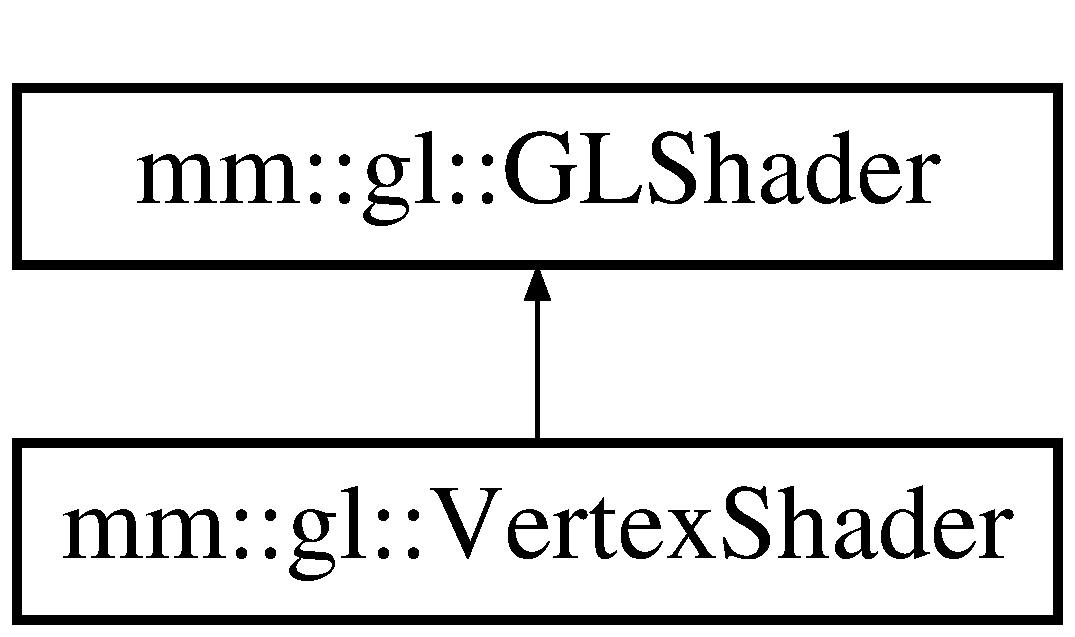
\includegraphics[height=2.000000cm]{classmm_1_1gl_1_1_vertex_shader}
\end{center}
\end{figure}
\subsection*{Public Member Functions}
\begin{DoxyCompactItemize}
\item 
\hypertarget{classmm_1_1gl_1_1_vertex_shader_a0b5794e93625ce7729811cf54d4f0243}{}{\bfseries Vertex\+Shader} (const std\+::string \&filename)\label{classmm_1_1gl_1_1_vertex_shader_a0b5794e93625ce7729811cf54d4f0243}

\end{DoxyCompactItemize}
\subsection*{Additional Inherited Members}


The documentation for this class was generated from the following files\+:\begin{DoxyCompactItemize}
\item 
src/core/mm\+\_\+opengl.\+h\item 
src/core/mm\+\_\+opengl.\+cc\end{DoxyCompactItemize}

%--- End generated contents ---

% Index
\backmatter
\newpage
\phantomsection
\clearemptydoublepage
\addcontentsline{toc}{chapter}{Index}
\printindex

\end{document}
